\documentclass[a4paper, titlepage, openright]{book}

\usepackage[english]{babel}
\usepackage{frontespizio}
\usepackage{amsmath}
\usepackage{amsthm}
\usepackage[linesnumbered,ruled,vlined]{algorithm2e}
\usepackage{textcomp}
\usepackage{mathtools, nccmath}
\usepackage[left=3cm,right=2cm,top=3cm,bottom=2cm]{geometry}
\usepackage{rotating}
\usepackage{subfigure}
\usepackage{url}
\usepackage{longtable}
\usepackage{amssymb}
\usepackage[mathscr]{euscript}
\usepackage{changepage}
\usepackage{graphicx}
\usepackage{float}
\usepackage{multirow}
\usepackage{algorithm2e}
\usepackage[normalem]{ulem}
\useunder{\uline}{\ul}{}

% force page number on page bottom part
\usepackage{fancyhdr} 
\fancyhf{}
\cfoot{\thepage}
\pagestyle{fancy}

% These Commands create the label style for tables, figures and equations.
\usepackage[labelfont={footnotesize,bf} , textfont=footnotesize]{caption}
\captionsetup{labelformat=simple, labelsep=period}
\newcommand\num{\addtocounter{equation}{1}\tag{\theequation}}
\renewcommand{\theequation}{\arabic{equation}}
\makeatletter
\renewcommand\tagform@[1]{\maketag@@@ {\ignorespaces {\footnotesize{\textbf{Equation}}} #1.\unskip \@@italiccorr }}
\makeatother
\setlength{\intextsep}{10pt}
\setlength{\abovecaptionskip}{2pt}
\setlength{\belowcaptionskip}{-10pt}

\renewcommand{\textfraction}{0.10}
\renewcommand{\topfraction}{0.85}
\renewcommand{\bottomfraction}{0.85}
\renewcommand{\floatpagefraction}{0.90}

% This styles the bibliography and citations.
\usepackage{natbib}
\setlength\bibindent{2em}
\makeatletter
\setlength{\bibsep}{0pt plus 0.3ex}

% redefine chapter -> no labeling with 1, 2, etc.
\newcommand{\mychapter}[2]{
    \setcounter{chapter}{#1}
    \setcounter{section}{0}
    \chapter*{#2}
    \addcontentsline{toc}{chapter}{#2}
}

% define maths operator
\DeclareMathOperator*{\argmax}{arg\,max}
\DeclareMathOperator*{\Var}{Var}

% This declares a command \Comment. The argument will be surrounded by /* ... */
\SetKwComment{Comment}{/* }{ */}

% define tools name
\newcommand{\motifgraph}{MotifGraph\xspace}
\newcommand{\grafimo}{GRAFIMO\xspace}
\newcommand{\crisprme}{CRISPRme\xspace}
\newcommand{\motifraptor}{MotifRaptor\xspace}
\newcommand{\crisprbean}{CRISPR-bean\xspace}

% table of contents will contain also subsections
\setcounter{tocdepth}{2}

% change Bibliography into References
\AtBeginDocument{\renewcommand{\bibname}{References}}

% set input and output for algorithm2e
\SetKwInput{KwInput}{Input}                
\SetKwInput{KwOutput}{Output} 

\begin{document}
% -----  title page
\begin{frontespizio}
	\Universita {Verona}
	\Dipartimento {Informatica}
	\Scuola {Ph.D. in Computer Science}
	\Annoaccademico {2022--2023}
	\Titoletto {Third Year Report}
	\Titolo {Predicting genetic variants imapct on genomic regulatory elements and CRISPR genome editing}
	\Candidato [VR456869]{Manuel Tognon}
	\NCandidato {Student}
	\NRelatore {Supervisor}{}
	\Relatore {Prof. Rosalba Giugno}
	\NCorrelatore {Cosupervisor}{}
	\Correlatore{Prof. Luca Pinello}
\end{frontespizio}
% ------  table of contents, index of figures and tables
\tableofcontents
\listoffigures
\listoftables
% ------ Introduction
\mychapter{1}{Introduction}
During the last decade, omics sciences have swiftly emerged as fundamental tools for informing medical decisions, serving as the foundational pillars supporting precision medicine \citep{ginsburg2009genomic}. Precision medicine is a rapidly progressing health care approach using individual-specific clinical, genetic, genomic, environmental and social information \citep{ginsburg2009genomic} to develop individual-tailored treatments. Although precision medicine encompasses a multidisciplinary approach, it largely relies on omics sciences to guide and enhance medical strategies and therapies. This technological progress had a profound impact, drastically reducing the costs associated with analyses involving omics data. Furthermore it empowered the accumulation of large dataset, even for individual patients \citep{voelkerding2009next}. Indeed, understanding the genetic basis of diseases is generally expected to lead to better characterized and tailored therapies \citep{ashley2016towards}. The evolution and enhancements in sequencing technologies brought about a profound transformation, substantially improving both the quantity and quality of available omics data. This facilitated the discovery of previously unknown causative genes \citep{ng2009targeted} and wider usage of omics data in medical decision-making processes \citep{ashley2010clinical, worthey2011making}. Collecting individual-specific omics data serves as a priceless asset for capturing the distinctive biological attributes, or \emph{biomarkers}, that define individuals and even offer insights into potential medical conditions, including diseases. The discovery of individual-specific biomarkers potentially causing medical conditions is the cornerstone of precision medicine. Among these biomarkers, genetic variants hold a pivotal position \citep{raphael2014identifying}. Genetic variants are differences in the DNA sequence when compared to a standard or reference sequence. They can occur naturally as mutations or alterations in the DNA sequence. They arise due to errors during different biological processes, such as DNA replication, \emph{mitosis} or \emph{meiosis}, or due to other DNA damages. The resulting mutations may undergo error-prone repair processes, particularly microhomology-mediated end joining \citep{sinha2017microhomology, seol2018microhomology}, leading to errors during other repair or replication mechanisms \citep{rodgers2016error}. Moreover, mutations in DNA sequences even can occur through the insertion or deletion of short DNA segments (indels), or large fragments consisting of thousands of nucleotides (structural variants). Genetic variants are common and fundamental aspects characterizing genetic diversity among individuals and populations \citep{siva20081000}. Some variants may have no noticeable effect on an individual's traits or health, while others can contribute to differences in susceptibility to diseases, response to medications, or various physical characteristics \citep{bodmer2008common, ingelman2018integrating, mitchell2007evolutionary}. Genetic variants may be located either within genes (coding regions), or in other genomic regions (non-coding regions). Historically, before the molecular causes were known, human genetics and clinical genetics studies focused on analyzing family pedigrees and inheritance descriptions to understand the occurrence of certain traits between single or groups of individuals. The advent of sequencing technologies allowed to study and discover the molecular mechanisms underlying the occurrence of traits or diseases in single individuals or populations. Furthermore, the recent advances in sequencing technologies significantly increased the throughput of sequencing experiments, providing huge amount of data. In this context, many international efforts, such as the 1000 Genomes Project \citep{siva20081000, 10002015global} and the Human Genetic Diversity Project \citep{cavalli2005human, bergstrom2020insights}, emerged to better study and understand the genetic diversity between human subjects and populations. Similarly, other consortia \citep{sherry2001dbsnp, landrum2020clinvar} collected variants data to discover potential associations between variants and traits or diseases. Simultaneously, several computational methods, such as variant calling \citep{mckenna2010genome} pipelines or genome-wide association studies (GWAS) \citep{uffelmann2021genome} to analyze and interpret variants-related data were proposed within the scientific community. However, the huge amount of data proved itself difficult to be fully exploited by using the common reference genome sequences. Reference genomes are commonly represented as strings, reporting the DNA sequence reconstructed from raw sequencing data. However, such representation cannot include the genetic variability and diversity present in genomes. Therefore, recently advanced data structures called genome graphs \citep{paten2017genome, garrison2018variation} have been introduced to represent in a single efficient data structure a genome and the genetic diversity among individuals and populations. Briefly, genome graphs are graph-based data structures, where nodes correspond to DNA sequences and edges describe allowed links between successive sequences. Paths through the graph, which may be labelled (such as in the case of a reference genome), correspond to haplotypes belonging to different genomes \citep{siren2020haplotype}. Despite integrating reference genome sequence data with variants allows to develop precision medicine-oriented methods, genome graphs overcome some limitations of these methods. In fact, genome graphs provide a framework handling variants from even thousands of individuals and complex variants combination as well as large events such as structural variants. Moreover, the recent release of the first draft of the human pangenome \citep{liao2023draft} holds promises in a wider adoption of these framework to study and represent the complexity of genetic variability.


in the complex landscape of cellular regulation, non-coding genetic variants frequently play important roles in the epigenetic machinery that governs the cellular environment \citep{maurano2012systematic}. While interpreting the functional impact of genetic variants mapped within coding regions on the cellular environment is often straightforward and widely explored in the existing literature, non-coding variants functional interpretation presents challenges.  We refer to the genomic regions governing the cellular environment as genomic regulatory elements (GREs). Currently, several computational tools designed to predict the effects of genetic variants within gene sequences are available to the scientific community.  However,  while these tools are valuable in assessing genetic variants impacts at broader level, they often fall short when it comes to accomodating the requirements of precision genomics.  In the evolving landscape of precision medicine, ther is a growing need for computational resources that can seamlessly  integrate individual-oriented aspects into their analyses.  Moreover, since genomics plays an increasingly central role in healthcare decision-making, the development of more individual centric computational tools becomes fundamental. We addressed these challenges by proposing innovative algorithms and computational tools tailored for the analysis of genetic variant impact on GREs and CRISPR genome editing, at broad and individual-specific levels. Our primary focus has been on creating haplotype- and individual-aware methods, aligning with the growing demand for individual-centric genomics applications.  Our research focused on developing novel algorithms designed to discover and find transcription factor binding sites (TFBSs) within DNA sequences, accounting for individual- and cell type-specific genetic variants.  We propose a novel computational model to represent TFBSs called MotifGraphs, which employs graph data structures to efficiently represent genetic diversity between binding sites from different individuals or cell types, without sacrificing interpretability.  To address the effects of genetic variants on TFBSs, we developed two novel algorithms \grafimo \citep{tognon2021grafimo} and \motifraptor \citep{yao2021motif}. \grafimo searches for occurrences of known TFBSs genome graphs \citep{paten2017genome}, while accounting for for individual haplotypes and genetic variants. \motifraptor predicts and annotates genetic variants impact on TFBSs integrating different omics data, such as chromatin accessibility, gene expression and GWAS summary statistics. Additionaly we introduced \crisprme \citep{cancellieri2023human}, a tool designed to CRISPR off-targets and avaluate the potential impact of individual genetic variants on target specificity.  Importantly,  \crisprme considers single-nucleotide variants, accomadate bona fide haplotypes and handles spacer:protospacer mismatches and bulges. This tool is specifically designed to perform individuals-oriented analyses, considering the wide genetic diversity present in different populations.

% ------ Genetic Variants
%
% ---> add figure with ref/alt allele - reference type (coding, non-coding) - SNV vs INS vs DEL - SVs
\mychapter{2}{Genetic Variants}
Genetic variants are modifications occurring in the DNA sequence within the genome of an organism. Mutations may result from errors during DNA replication processes, \emph{mitosis}, \emph{meiosis}, or other forms of DNA damage (such as the formation of pyrimidine dimers induced by exposure to ultraviolet radiation). In this discussion, we treat genetic variants and mutations as synonymous terms. Mutations may undergo error-prone repair processes, such as microhomology-mediated end joining (MEMJ) \citep{sinha2017microhomology, seol2018microhomology}, resulting in errors during repair and replication of the original DNA sequence \citep{rodgers2016error}. Mutations may consist in substitutions of single nucleotide in the sequence, as well as in insertions or deletions of DNA segments. The different versions of the same variant are referred to as \emph{alleles}. We define the variant observed in the reference (original) DNA sequence \emph{reference allele}, and any other distinct version from the reference is called \emph{alternative allele}.
% ---> add figure reference
The impact of mutations on the phenotype depends on several factors, ranging from the organism's genomic environment to the social environment in which the organism is located. While some genetic variants may not impact the phenotype, others may introduce differences in the organism's susceptibility to disease, response to drugs and treatments, or physical characteristics \citep{bodmer2008common, ingelman2018integrating, mitchell2007evolutionary}. Furthermore, mutations furnish the raw material upon which evolutionary forces, such as natural selection, can act \citep{akey2004population, teotonio2009experimental}. Genetic variants may occur either within gene sequences (coding regions), or outside genes (non-coding regions).  Mutations occurring in coding regions may have either advantageous or deleterious consequences on the organism's phenotype, by altering the gene product. Although variants in non-coding regions do not alter gene sequences, they still may impact gene products and the organism's phenotype \citep{zhang2015non}. 

% ----- Genetic Variants Genesis
\section{Genetic Variants Genesis}
DNA may undergo naturally occurring or artificially induced modifications resulting in mutations. Mutations can occur spontaneously in nature, as result of exposure to chemical or physical agents increasing the mutation rate in DNA sequences called \emph{mutagens}, or induced experimentally using laboratory protocols (e.g. CRISPR genome editing \citep{cong2013multiplex}). Variants can be categorized in four classes depending on the process that induced the emergence of the mutations: (i) spontaneous mutations, (ii) error-prone translesion synthesis, (iii) errors introduced during DNA repair processes, and (iv) induced mutations resulting from exposure to mutagens. Spontaneous mutations occur randomly across the genome sequence even in healthy cells. Spontaneous mutations are caused by different random events, such as incorrect base pairing during DNA replication caused by tautomerism \citep{podolyan2003ab}, slipped-strand mispairing during replication \citep{levinson1987slipped}, deamination \citep{duncan1980mutagenic}, or depurination \citep{kunkel1984mutational}. Some spontaneous mutations are induced by error-prone replication mechanisms (translesion synthesis), acting on damaged DNA. While naturally occurring damages to the DNA sequence, such as double-strand breaks, exhibit low frequency, their repair processes often introduces mutations. A prominent pathway for repairing double-strand breaks is non-homologous end joining (NHEJ) \citep{weterings2008endless}. In NHEJ, a few nucleotides are removed to facilitate the imprecise alignment alignment of the broken ends for rejoining, and subsequently, additional nucleotides are added to fill the remaining gaps. However, as consequence NHEJ introduces insertions or deletions into the original DNA sequence \citep{weterings2008endless}. Finally, mutations may be induced by the exposure of DNA sequences to mutagens, such as chemical (nitrous acid, hydroxylamine, alkylating agents, etc.) or radiation (UV light, ionizing radiation) agents. Importantly, some mutagens are commonly found in the environment, and organisms are normally exposed to their action.

% ----- Classifying Genetic Variants
\section{Classifying Genetic Variants}
During the years have been proposed different methods to classify genetic variants based on their inheritance, the modifications induced to the DNA structure, their location, and their impact on the gene product.

% ---- Classifying Genetic Variants by their inheritance
\subsection{Classifying Genetic Variants by their inheritance}
In multicellular organisms, variants can be categorized in \emph{germline} mutations, which can be inherited by descendants, and \emph{somatic} mutations, which generally are not transmitted to descendants. Diploid organisms, such as human, possess two copies of each chromosome, one inherited from the father, the other from the mother. Depending on the occurrence of mutations on each chromosome, variants can be classified in three types: (i) heterozygous mutations, when only one copy of the chromosomes carries the alternative allele, (ii) homozygous mutations, when both copies carry the same alternative allele, and (iii) compound mutations, when the two copies carry different alternative alleles. Germline mutations occurring in the reproductive cells of an individual result in constitutional mutations in the offspring, spread in every organism's cell. Importantly, germline mutations have the potential to be transmitted through successive generations. A newly occurring germline mutation, not inherited from parents is defined \emph{de novo} mutation. Somatic mutations do not affect the germline and are generally not transmitted to descendants. However, they are inherited by all the progeny derived from a mutated cell within the same organism during mitosis. Somatic mutations are often linked to deleterious consequences for the cell, such as cancer \citep{martincorena2015somatic}. 

% ---- Classifying Genetic Variants by their impact on DNA sequence structure
\subsection{Classifying Genetic Variants by their impact on DNA sequence structure}
Genetic variants can be classified in three classes based on the structural modification they induce to the DNA sequence: (i) single nucleotide variants (SNVs), (ii) insertions and deletions (indels), and (iii) structural variants.

% --- Single nucleotide variants
\subsubsection{Single Nucleotide Variants}
A single nucleotide variant (SNV) denotes a germline substitution involving a single base at a precise position within the genome. For example a \texttt{G} occurring at a specific genome location may be replaced by an \texttt{A}. In this example the two alleles (nucleotide variations) are \texttt{G} (reference allele) and \texttt{A} (alternative allele). SNVs exhibits an allele frequency $< 1\%$. When single nucleotide substitutions show a frequency $\geq 1\%$ in the general population they are defined Single Nucleotide Polymorphisms (SNPs). The human genome within the global population has revealed the presence of over 600 million SNPs, which occur more frequently in non-coding regions than in coding. Human populations exhibit variations, leading to the prevalence of certain SNP alleles in specific geographic or ethnic groups while being comparatively rare in others. However, this variation is not frequent on a global scale \citep{bergstrom2020insights}. Within a population, SNPs can be characterized by their minor allele frequency (MAF). MAF is defined as the lowest frequency of an allele at a locus observed in a particular population. This frequency represents the lesser of the two allele frequencies for single-nucleotide polymorphisms.

% --- Indels
\subsubsection{Indels}
Indel denote the insertion or deletion of nucleotides within a genome. Indels with length $\geq 50$ bp are often referred to as structural variants. Indels are used as genetic markers in natural populations, particularly in phylogenetic studies \citep{vali2008insertion}. Between $16\%$ and $25\%$ of all sequence polymorphisms in humans are likely to be represented by indels \citep{mills2006initial}. In most deeply studied genomes, as the human genome, indels frequency is notably lower compared to that of SNPs, except in the vicinity of highly repetitive regions, such as homopolymers and microsatellites.

% --- Structural Variants
\subsubsection{Structural Variants}
Structural variants refer to diverse alterations in the chromosome structure of an organism. Historically, structural variants were defined to affect sequences of length between $\sim$1 Kb to 3 Mb \citep{feuk2006structural}. However, recently their range has been expanded to consider events affecting sequences $>50$ bp \citep{alkan2011genome}. Approximately 13\% of the human genome is structurally variant in the normal population \citep{sudmant2015integrated}. Furthermore, there are several evidences suggesting that structural variants can encompass millions of nucleotides of heterogeneity within each genome, potentially playing a pivotal role in human diversity and susceptibility to diseases. Many structural variants are linked to diseases \citep{lakich1993inversions}. Structral variants encompass several types of variations, such as inversions, copy-number variants (CNVs), translocations, deletions, insertions, and duplications. Deletions, insertions and duplications are particular cases of CNVs.  Inversions are chromosomal rearrangements wherein a chromosomal segment undergoes an inversion, flipping its original position. Inversions occur when a chromosome experiences two breaks along its arm, and the DNA segment between the breakpoints inserts itself in the opposite direction, within the same chromosome arm. Generally, breakpoints occur in regions rich of repetitive nucleotides. Importantly, inversions may flip or even break genes or regulatory elements sequences \citep{puig2015human}. Inversions can occur through different mechanisms, such as chromosomal breakage and repair, or non-homologous end joining. There are two types of inversions: paracentric inversions, which do not involve chromosome's centromere, and pericentric, which span the centromere and have breakpoints in each chromosome's arm. In CNVs sections of an organism's genome are duplicated or deleted, resulting in variations in the number of repeated nucleotide sequences among individuals \citep{mccarroll2007copy, alkan2011genome}. Therefore, this structural variants involves insertions or deletions $>$50 bp in the genome. CNVs represent a fundamental aspect of genomic diversity, encompassing $4.8-9.5\%$ of the genome in human \citep{zarrei2015copy}. Translocations, instead, are structural variants leading to atypical rearrangements of chromosomes. There exist two types of translocations: reciprocal and Robertsonian translocations. The former occurs when non-homologous chromosomes exchange DNA fragments between each other. Robertsonian translocations, instead, occur when two non-homologous chromosomes become attached. Importantly, translocations can result in the fusion of two genes(\emph{gene fusion}) or regulatory elements, otherwise separate. Translocations may be balanced, when the exchange of genetic material is even, or unbalanced. The latter may result in extra or missing genes or regulatory elements on the donor/receiver chromosome. 

% ---- Classifying Genetic Variants by their location
\subsection{Classifying Genetic Variants by their location}
Another method to distinguish genetic variants is based on their location across the genome. \emph{Coding} genetic variants occur within the coding sequence of genes (exons), while \emph{non-coding} variants occur in non-coding sequences of genes (introns) or intergenic regions. While coding variants may directly impact the gene product, non-coding variants may still affect gene splicing, gene expression levels, or the gene regulatory mechanisms perturbing the cell environment \cite{li2016rna, maurano2015large}. In particular, non-coding variants occurring within large and small regulatory elements, such as enhancers or transcription factor binding sites, have been shown to significantly impact gene expression levels and regulation \citep{de2006regulatory, wienert2015editing}, and have been linked to increased susceptibility to some diseases, such as cancer \citep{weinhold2014genome}. Coding variants may affect the gene product, potentially modifying the sequence of the resulting protein. The impact that such mutations may have on the gene product provides another method to classify genetic variants.

% ---- Classifying Genetic Variants by their impact on gene product
\subsection{Classifying Genetic Variants by their impact on gene product}
Coding variants may or may not impact the gene product. Considering SNVs, in the former case variants are defined \emph{synonymous substitutions}, in the latter \emph{nonsynonymous substitutions}. Despite the different nucleotide, synonymous substitutions do not change the amino acid encoded by the affected codon. Nonsynonymous substitutions, instead, alter the gene product either changing the amino acid encoded by the affected codon (\emph{missense}), or inserting a premature stop codon (\emph{nonsense}). Indels, in contrast, if their length is a multiple of 3, they can either eliminate or add one or more amino acids to the gene product. However, if their length is not a multiple of 3, they may induce a reading frame shift, potentially leading to the disruption of the gene product or the introduction of a premature stop. Structural variants are excluded from this classification.

% ----- Combining variants: the concept of Haplotype
\subsection{Combining variants: the concept of Haplotype}
Clusters of alleles inherited from a single parent are defined \emph{haplotypes}. Typically, in organisms which inherit the genetic material from two parents is organized in two sets of pairwise chromosomes transmitted to the offspring. A diploid set encompasses pairs of chromosomes, whereas a haploid set comprises only one half of each pair. The haploid genotype focuses on individual chromosomes rather than pairs, encompassing either all chromosomes from one parent or even a specific segment. The term haplotype has multiple applications. It refers to a collection of specific alleles clustered within tightly linked genes on a chromosome, likely to be inherited together and preserved across generations. It also indicates sets of linked SNP alleles statistically associated and likely to occur together. Identifying these associations, along with a few alleles of a specific haplotype sequence, is often used to locate other nearby polymorphic sites on the chromosome. Importantly, haplotypes are crucial to investigate the genetics of common diseases and traits, and their occurrence across different human groups or populations. The crucial importance of haplotypes is highlighted by international efforts such as the International HapMap Project \citep{gibbs2003international}, whose aim was to develop a haplotype map of the human genome, describing common patterns of human genetic variation and diversity.

% ----- Interpreting and understanding Genetic Variants impact 
\section{Interpreting and understanding Genetic Variants impact}
Advancements in sequencing technologies have revolutionized the accumulation of extensive data on genetic variants and genomic diversity, with a primary focus on the human genome. Notably, international initiatives like the 1000 Genomes Project \citep{siva20081000, 10002015global} and the Human Genome Diversity Project \citep{bergstrom2020insights} have diligently worked towards capturing the spectrum of genetic diversity across individuals and populations. A wealth of experimentally validated data is stored in various databases, such as dbSNP \citep{sherry2001dbsnp}, ClinVar \citep{landrum2020clinvar} or COSMIC \citep{bamford2004cosmic}, linking known variants to genetic traits or diseases. These resources are fundamental tools to understand and interpret the potential impact of genetic variants on the genetic landscape. Given the intricate nature of sequencing data, several computational pipelines have emerged to sift through this vast information, identifying variants from raw sequencing data. Variant calling tools, such as the Genome Analysis Toolkit (GATK) \citep{mckenna2010genome}, Strelka \citep{kim2018strelka2}, Varscan \citep{koboldt2012varscan} or FreeBayes \citep{garrison2012haplotype}, analyze sequencing data to unveil the variants present within an individual's genome, for example. Simultaneously, methodologies and pipelines have been developed to explore potential associations between specific variants and diseases, such as genome-wide association studies (GWAS) \citep{uffelmann2021genome}, or to predict their functional impact on the molecular mechanisms governing the cell \citep{mclaren2016ensembl}. These studies and achievements unraveled the intricate complexity and diversity inherent in the human genome. However, representing such intricacy using the conventional reference genome sequences becomes challenging. To address this limitation, complex data structures known as genome graphs \citep{paten2017genome} have been recently introduced. These graphs offer a comprehensive framework to embed the genetic diversity within individuals and populations, presenting a novel, graph-based data structure. This innovative approach is poised to provide a more nuanced understanding of the intricate tapestry of the human genome. Genome graphs also provide a comprehensive and efficient framework to consider individual- and population specific mutations, supporting the shift towards precision medicine-oriented approaches. Moreover, the recent release of the first draft of the human pangenome reference \citep{liao2023draft} testifies how the shift towards the use of frameworks embedding genetic variation are more and more supported by the scientific community.

% ---- Identifying Genetic Variants
\subsection{Identifying Genetic Variants}
Identifying and interpreting the consequences of variants occurrence is crucial to unveil the molecular mechanisms underlying several common and rare traits and diseases. Historically, variants and in particular SNVs were identified employing techniques such as mass spectrometry, or single-strand conformation polymorphism \citep{orita1989detection}. However, this methods allowed to analyze a few variants. DNA sequencing technologies almost completely replaced these protocols. In fact, sequencing technologies allow to recover and study the entire variation of genomes at lower costs. To analyze sequencing data and \emph{call} variants, during the last decades have been developed several \emph{variant calling} pipelines and methods. Variant calling pipelines encompass three main steps: (i) genome sequencing, (ii) sequence alignment to a reference genome, and (iii) variants identification. During genome sequencing the DNA is sequenced by sequencer machines, which reconstruct the genomic sequences splitting it in short or long overlapping and redundant sequences, called short or long reads, respectively. The resulting reads are stored in FASTQ files (\textbf{Appendix \ref{section:fastq-format}}). The generated reads are then mapped to a reference genome. Aligning reads helps identify the genomic locations of these reads within the genome, allowing to reconstruct the original genomic sequence and enables the identification of genetic variations, such as SNPs, indels, and structural variations, during the variant identification. The accurate alignment of reads is essential for downstream analyses like variant calling and understanding the functional implications of genetic variations in the context of the reference genome. Aligned reads are stored in BAM or CRAM files (\textbf{Appendix \ref{section:bam-format}} and \textbf{\ref{section:cram-format}}). Various algorithms and tools, like Bowtie \citep{langmead2012fast}, BWA \citep{li2009fast}, and HISAT \citep{kim2019graph}, are commonly used for efficient and accurate sequence alignment. The last step focuses on identifying and characterizing genetic variants in the sequenced genome. Once the reads are aligned, variant calling algorithms are employed to detect differences between the sample and the reference. These algorithms analyze the aligned reads to identify positions where the sample's sequence differs from the reference genome. Variant calling algorithms may apply filters on the identified variants to remove false positives and improve the accuracy of variant calls. Moreover, they can annotate the identified variants, adding information such as their genomic location, functional impact, and population frequency. Variant callers can also call determines the specific genetic makeup (\emph{genotype}) of an individual at each variant position. The identified variants are generally stored in VCF (Variant Calling Format) files. Variant calling is crucial for understanding the genetic differences between individuals, populations, or disease states. Multiple tools, including GATK \citep{mckenna2010genome}, SAMtools \citep{li2009sequence}, Strelka \citep{kim2018strelka2} and VarScan \citep{koboldt2012varscan}, are commonly used for variant calling. Accurate and reliable variant calling is essential for studies focused on identifying disease-causing mutations, understanding genetic diversity, and uncovering associations between genetic variants and specific traits or diseases. Furthermore, variant calling constitutes a fundamental tool to recover individual and population-specific genetic diversity, playing a pivotal role in defining precision medicine oriented computational methods.

% --- The Variant Calling Format (VCF)
\subsubsection{The Variant Calling Format (VCF)}
The Variant Call Format (VCF) is a standard file format used for storing information about genetic variants identified through variant calling analyses. VCFs are plain text file providing several and different information organized in fields regarding the reported variants. Due to their dimensions, VCFs are often compressed. VCFs have two main components: (i) a header and (ii) a body. The header contains metadata and information about the reference genome, describes the sample information, file creation date, the tools used for variant calling, and specifies the version of the VCF format. The body comprises rows of variant records, each representing a genetic variant.  Variants records consist of eight mandatory tab-separated fields, along with an unlimited number of optional columns (\textbf{Table \ref{table:vcf-fields}}). The fields in a variant record provide detailed information about the variant. The VCF file format is versatile and supports the representation of a wide range of genetic variants, including SNPs, indels, and structural variants. It has become a standard for exchanging variant information across different bioinformatics tools and databases, facilitating the sharing and integration of genomic data in research and clinical settings.
 
% - table: Variant Calling Format (VCF) fields
\begin{table}[h!]
	\centering
	\begin{tabular}{|p{1cm}|p{2cm}|p{7cm}|p{2cm}|}
		\hline
		\textbf{Field}& \textbf{Field name}& \textbf{Description}& \textbf{Type}\\
		\hline
		1 & CHROM & The identifier of the sequence on which the variant has been called, commonly denoting the chromosome name & Mandatory\\
		\hline
		2 & POS & The variant's position relative to the reference sequence & Mandatory\\
		\hline
		3 & ID & Variant's identifier & Mandatory\\
		\hline
		4 & REF & Reference allele & Mandatory\\
		\hline
		5 & ALT & Altrenative allele & Mandatory\\
		\hline
		6 & QUAL & The assigned quality score for the inference of the called allele & Mandatory\\
		\hline
		7 & FILTER & A flag value indicating whether the variant has successfully passed the filtering steps & Mandatory\\
		\hline
		8 & INFO & An expandable list of key-value pairs describing the variant, following the syntax <key>=<data>[,data] & Mandatory\\
		\hline
		9 & FORMAT & Sample's related fields & Optional\\
		\hline
		+ & SAMPLE & Values are provided for the FORMAT fields for each described sample & Optional\\
		\hline
	\end{tabular}
	\caption[Variant Calling Format (VCF) fields]{\textbf{Variant Calling Format (VCF) fields.} The table outlines the eight mandatory fields of a VCF file along with two frequently used optional fields (FORMAT and SAMPLE)}
	\label{table:vcf-fields}
\end{table}

% ---- Genetic Variants Databases
\subsection{Genetic Variants Databases}
The recent strides in sequencing technologies have substantially augmented the throughput of sequencing experiments, generating vast datasets. In response to this, numerous global initiatives, exemplified by the International HapMap Project \citep{gibbs2003international, international2005haplotype}, the 1000 Genomes Project (1KGP) \citep{siva20081000, 10002015global} and the Human Genetic Diversity Project (HGDP) \citep{cavalli2005human}, have surfaced. These endeavors aim to delve deeper into the genetic diversity among human individuals and populations. Similarly, consortia like dbSNP \citep{sherry2001dbsnp} and ClinVar \citep{landrum2020clinvar} have aggregated variant data to explore potential associations between genetic variants and various traits or diseases. The HapMap project was among the first initiative to perform large scale experiments to uncover human genetic diversity. Their goal was to construct a haplotype map of the human genome, elucidating potential prevalent variants patterns among population. In fact, while generally shared across populations, haplotypes can exhibit significant variations in frequency. The primary objective of 1KGP was to identify common genetic variants with frequencies of at least 1\% within the studied populations (SNPs). Leveraging advancements in sequencing technology, the project pioneered large-scale sequencing of genomes from a diverse group of individuals, creating a comprehensive database on human genetic variation \citep{fairley2020international}. While the cost of deep sequencing for the extensive number of samples was still prohibitive, the genome's specific regions typically harbor a limited number of haplotypes. By aggregating data across samples, the project efficiently detected the majority of variants in a region. The initial plan aimed to achieve 4x genomic coverage for each sample, recognizing that this depth might not unveil all variants in each sample but could detect most variants with frequencies as low as 1\%. In the project's final phase, data from 2,504 samples from 26 populations were amalgamated, enabling accurate genotyping at all discovered variant sites. The multi-sample strategy, coupled with genotype imputation \citep{li2009genotype}, facilitated determining samples' genotype, even for variants not covered by sequencing reads. However, 1KGP dataset does not cover all human populations. To fill this gap the 1KGP data have been extended performing further experiments as well as including data produced by other consortia, such as HGDP \citep{bergstrom2020insights}. Similarly to 1KGP, HGDP aim was to identify and map genetic variation and diversity among human populations. 1KGP and HGDP could be considered complementary datasets. In the meantime, other consortia focused on collecting the variants experimentally identified in databases. dbSNP \citep{sherry2001dbsnp} is a publicly accessible repository providing comprehensive information on genetic variation. It functions as a unified database containing all identified genetic variations, facilitating the investigation of a broad range of genetically influenced natural phenomena. Despite its name suggests a focus solely on SNPs, dbSNP encompasses a broader spectrum of molecular variations \citep{sherry1999dbsnp}, including SNPs and short indels for example. dbSNP plays a crucial role in guiding applied research in fields such as exploring variants-trait associations \citep{kitts2002single}. While dbSNP reports broader information about genetic variants, ClinVar \citep{landrum2020clinvar} details variants-traits association focusing on the clinical significance of such associtions. ClinVar main purpose is to streamline access to information and facilitate communication regarding the relationships posited between human genetic variations and observed health conditions, along with the historical context of these interpretations. These repositories provide valuable resources providing several data to analyse the potential impact of genetic variation on the cell environment. By providing raw data and functional details, these databases are significant resources, fundamental to develop precision medicine-oriented methods that consider genetic variants. 

% ---- Discovering Variants - Trait associations
\subsection{Discovering Variants - Trait associations}
Once identified, a key question is to discover whether our variants are linked to a particular trait, or to predict their potential impact on the cellular environment. Genome-wide association studies (GWAS) \citep{uffelmann2021genome} provide answers to the first question. GWAS is an observational investigation of a comprehensive set of genetic variants across different individuals to identify potential associations with a particular trait or disease. These studies predominantly focus on relationships between SNPs and major human diseases, although they are equally applicable to other genetic variants, such as indels for example. GWAS typically involve large cohorts of individuals, comparing the genomes of those with a particular trait or disease to those without. Case-control designs are common, where individuals with a specific trait or disease (cases) are compared to those without (controls). To collect GWAS data high-throughput genotyping technologies, such as SNP arrays, are employed to assay hundreds of thousands to millions of SNPs across the genome. To identify between genetic variants and traits, GWAS employ statistical methods. Correction for multiple testing is crucial to minimize false-positive results. Linkage Disequilibrium analysis helps identify blocks of correlated genetic variants, providing insights into the genomic regions associated with the trait of interest. Importantly, population stratification must be carefully addressed to avoid spurious associations due to differences in genetic ancestry. Different computational tools, such as PLINK \citep{purcell2007plink} or SNPTEST \citep{marchini2007new}, have been developed to carry out GWAS. While other methods focus on a limited number of predefined genetic regions, GWAS explores the entire genome. Consequently, GWAS adopts a non-candidate-driven approach, in contrast to gene-specific candidate-driven studies. However, while GWAS identifies SNPs and other DNA variants associated with a disease, it does not independently determine which impact the variants have on the cell environment and which gene/genomic element is causative of the investigated trait/disease. Functional annotation annotates and interprets the functional significance of variants identified during GWAS. Several databases and tools have been developed for this task. For example PROVEAN \citep{choi2015provean} and VEP \citep{mclaren2016ensembl} predict the impact of variants on gene products, while RegulomeDB \citep{boyle2012annotation} investigates the impact of genetic variants on genomic regulatory elements.

% ---- Limitations of current analysis methods
\subsection{Limitations of current analysis methods}
As described throughout this chapter, over the last decades have been proposed different methods and computational tools to analyze, assess and predict the impact of genetic variants on the cellular environment. However, these methods may have limitations and may not fully exploit the information of the analyzed variants data. Methods employing variants to enrich the reference genome sequence may lose or not consider simultaneously SNVs and indels, because the latter may break the sequence coordinate system. Moreover, these methods generally are not able to consider large variant events, such as structural variants, and complex SNVs-indels combinations in their analyses. Most methods ignores haplotypes and may introduce recombinant sequences not observed in the data. Furthermore, most methods are not scalable when analyzing large set of individual-specific data and do not perform population-based analyses. These limitations may impact the shift towards the development of precision medicine-oriented methods. The recent advent of genome graphs \citep{paten2017genome} presents a powerful framework for representing genomes alongside their complete genetic variation and diversity. Importantly, genome graphs may enhance precision medicine-oriented analyses by encapsulating the genetic diversity of numerous samples, ranging from several to thousands, within a unified data structure \citep{yu2023human}. The subsequent chapter delves into the details of the genome graphs data structure, shedding light on recent advancements and exploring the prospective enhancements this data structure could bring to the forefront of developing novel methods for analyzing the impact of genetic variants on cellular processes.


% ------ Genome Graphs
\mychapter{3}{Genome Graphs}
The use of the human reference genome as a basis for studying genetic variations in other human genomes introduces a significant challenge known as reference allele bias. This bias, stemming from mapping errors during sequencing experiments, tends to underreport data that deviates from the reference allele \citep{degner2009effect, brandt2015mapping}. Structural variations pose a particular challenge, requiring distinct algorithms for their detection, due to their absence from the reference \citep{sudmant2015integrated}. To address these limitations, the field of genome inference is moving towards unbiased \emph{de novo} assembly for individual samples and developing richer reference structures that more comprehensively represent population variations, such as graph-based reference structures. This transition towards graph-based reference structures is particularly evident in human genomics, signaling a shift in the approach to variant calling and genome analysis. Genome graphs \citep{paten2017genome} offer a revolutionary approach to address the limitations of traditional linear genome representations (\textbf{Figure \ref{fig:genome-graph}}). Stemming from the concept of sequence graphs \citep{paten2017genome}, genome graphs provide a versatile framework to encapsulate the genetic diversity inherent in multiple individual genomes within a unified data structure. A sequence graph (\textbf{Figure \ref{fig:genome-graph} (A)}) is essentially a bidirectional graph where nodes correspond to DNA fragments, and edges signify the adjacency between different segments in a sequence. These edges connect the terminus of one DNA segment to the inception of another, bearing a label denoting a string of DNA (which can be empty). Consequently, traversing the graph through adjacent nodes linked by edges allows for the retrieval of genetic sequences. Originally conceived to succinctly represent multiple sequences sharing variations, sequence graphs have found extensive applications. Mainly, sequence graphs serve as efficient data structures for storing diverse genetic information and have been instrumental in tasks such as the succint representation of multiple sequence alignments \citep{lee2002multiple,paten2014unifying}. Therefore, genome graphs can be perceived as an evolution of bidirectional sequence graphs. Notably, genome graphs offer a comprehensive representation enriched with a collection of paths encapsulating genome sequences across a population of individuals (\textbf{Figure \ref{fig:genome-graph} (B)}). These graphs serve as a compact yet robust depiction of genetic variation within a population, encompassing structural variants, such as inversions and duplications \citep{paten2017genome}. Formally, a genome graph is defined as $G = (N, E, P)$, where $N = \{n_{1}, n_{2}, \ldots, n_{k}\}$ denotes the set of nodes representing DNA segments, $E = {e_{1}, e_{2}, \ldots, e_{w}}$ denotes the set of edges connecting nodes, and $P = {p_{1}, p_{2}, \ldots, p_{q}}$ comprises the set of paths embedded in $G$. Each path $p \in P$ represents one of the embedded sequences or genomes within the genome graph. Each node in the graph corresponds to a DNA segment constructed from the alphabet $\Sigma = \{\text{\texttt{A}}, \text{\texttt{C}}, \text{\texttt{G}}, \text{\texttt{T}}, \text{\texttt{N}}\}$. Therefore, by incorporating a multitude of paths, genome graphs offer a holistic view of genomic diversity within a population of individuals, enabling the representation of complex genetic structures and facilitating comprehensive genetic analyses. 
%
% - figure: The genome graph and sequence graph data structures
\begin{figure}[!]
	\centering
	\includegraphics[width=\textwidth]{figures/genome-graph.png}
	\caption[The genome graph and sequence graph data structures]{\textbf{The genome graph and sequence graph data structures. (A)} A sequence graph, denoted as $S$, is constructed from three sequences: $s_{1}$ = \texttt{TCGTAGAAATAACGCGGC}, $s_{2}$ = \texttt{TCGTAGAAAACGGC}, and $s_{3}$ = \texttt{TCGTAGCGTACGACGGC}. By tracing the purple path within the graph, the original sequence $s_{1}$ can be reconstructed, while following the yellow path yields the reconstructed sequence $s_{2}$. It's noteworthy that in sequence graph $S$, the edges are not labeled, although in general, they could carry labels for additional information. \textbf{(B)} Visualization of Genome Graphs data structure, with each color representing a distinct path within the graph. Each path delineates the genomic sequence of an individual genome encoded within the Genome Graph structure. This comprehensive representation facilitates the simultaneous depiction of multiple genetic sequences, enabling the exploration of genetic diversity and complexity across individuals within a population.}
	\label{fig:genome-graph}
\end{figure}
%
Traversal through the graph is facilitated in both forward and reverse directions, presenting two distinct "entry points" for each node $n \in N$ (\textbf{Figure \ref{fig:genome-graph-visits} (A)}). When traversing a node in the reverse direction, the DNA fragment associated with the node is read as its reverse complement (\textbf{Figure \ref{fig:genome-graph-visits} (B)}). Edges within the genome graph signify adjacency between the DNA fragments of the nodes they connect. Consequently, long sequences are implicitly encoded by concatenating the fragments of adjacent nodes. Similar to nodes, edges can be traversed in the reverse direction, enabling comprehensive exploration of genetic sequences. Moreover, to increase graph's compactness, genome graphs are capable of accommodating cycles to represent repetitive segments across the embedded sequences (\textbf{Figure \ref{fig:genome-graph-visits} (C)}). Genome graphs usually accomodate different types of cycles: regular cycles where a node $n_{i}$ can be reached from $n_{i}$, reversing cycles, where $n^{r}_{i}$ is reachable from $n_{i}$, and instances of non-cyclic reversal (\textbf{Figure \ref{fig:genome-graph-visits} (D)}), where both $n_{i}$ and $n^{r}_{i}$ are accessible from another node $n_{j}$. In the context of representing genomes for a population of individuals, paths within genome graphs correspond to the genomic sequences of each subject. Variants manifest as bubbles in the graph, creating diverging paths anchored by a common start and end sequence on the reference \citep{paten2018superbubbles} or a shared DNA segment. Genome graphs provide an efficient and compact framework to represent and encode the genetic diversity observed within populations of individuals. Notably, genome graphs offer a groundbreaking framework that expands classical omics analysis to encompass not only simple variations like SNPs and indels, but also more complex genetic alterations such as large indels, SNP-indel combinations, and structural variants. This versatility makes genome graphs a powerful tool for capturing the intricate genetic landscape present in diverse populations. In recent years, there has been a noticeable shift towards adopting genome graph-based representations of genomes over traditional genome assemblies for genetic data analysis \citep{hurgobin2017snp}. This transition has been further accelerated by the emergence of several consortia dedicated to constructing and releasing population-based \citep{gao2023pangenome} or comprehensive pangenomes \citep{wang2022human}, with these pangenomes being represented as genome graphs. Notably, a significant milestone was reached with the release of the first draft of a genome-graph-based human reference genome, known as the pangenome reference \citep{liao2023draft}. This landmark achievement underscores the growing recognition and adoption of genome graph technology in genomic research, promising a more comprehensive and accurate understanding of genetic variation and its implications. Furthermore, genome graphs  hold great promises in facilitating the shift towards the adoption of precision medicine-oriented approaches to analyse genetic data accounting for genetic diversity across individuals and populations \citep{yu2023human}. However, scaling pangenomes' genome graph data structures to accommodate hundreds of genomes poses a  significant computational challenge. In recent years, numerous software tools have been developed to construct and analyze genome graph-based pangenomes \citep{andreace2023comparing}. While construction procedures and implementations may vary, they collectively underscore how genome graphs significantly enhance a wide array of genomic analyses. These improvements are evident in various areas, including high-quality short read mapping \citep{siren2021pangenomics}, accurate genotyping of SNPs, indels, and structural variants (SVs) \citep{ebler2022pangenome}, RNA-seq mapping \citep{liao2023draft}, and de novo variant calling \citep{garrison2018variation}. The following sections delve into some of the prominent methods for constructing genome graph-based pangenomes and elucidate their potential to enhance genetic data analysis.

% - figure: Traversing the genome graph along the embedded paths
\begin{figure}[!]
	\centering
	\includegraphics[width=\textwidth]{figures/genome-graph-visits.png}
	\caption[Traversing the genome graph along the embedded paths]{\textbf{Traversing the genome graph along the embedded paths. (A)} A genome graph provides multiple traversal possibilities based on its nodes, edges, and paths. \textbf{(B)} By following the red path, the forward sequence \texttt{ATATTCCAACTCTCTG} can be reconstructed, while tracing the green path yields its reverse complement. \textbf{(C)} Genome graphs accommodate ordinary cycles and reversing cycles. The red path reveals an ordinary cycle at node 12, while the green path highlights a reversing cycle at node 14, where an edge exits and re-enters the node, necessitating consideration of the DNA label as its reverse complement. Such intricate graph structures efficiently represent complex genomic rearrangements, such as sequence duplications (as seen in the red path case) or inversions (as observed in the green path case). \textbf{(D)} Genome graphs may also exhibit non-cyclic instances of reversal; for instance, node 13 can access both the forward DNA fragment of node 15 (via the red path) and its reverse complement (via the green path).}
	\label{fig:genome-graph-visits}
\end{figure}

% ----- Methods to Construct Genome Graphs
\section{Methods to Construct Genome Graphs}
In recent years, we have witnessed a dynamic landscape of research endeavors aimed at developing methods and data structures tailored to construct and represent pangenomes as genome graphs \citep{computational2018computational,andreace2023comparing}. This surge in activity reflects the growing recognition of genome graphs as powerful tools for capturing the complexity and diversity inherent in genomic data. Among the diverse array of approaches currently available, several notable methods have garnered attention for their efficacy in handling large datasets and facilitating efficient representation of genome graphs. The Variation Graph Toolkit \citep{garrison2018variation}, for instance, has emerged as a foundational tool in the field, offering robust capabilities for constructing genome graphs that encompass intricate genetic variations. Notably, the Variation Graph Toolkit provides a comprehensive suite of tools for analyzing genomic sequence data utilizing the genome graph data structure. The resulting variation graphs (VGs) can be constructed either from user-provided data or from precomputed graphs in a variety of supported graph formats. With the Variation Graph Toolkit, users can manipulate and visualize VGs, enabling detailed exploration and analysis of genomic variations. The introduction of VGs represents a significant advancement in genomic data representation. By encapsulating the complexity introduced by genetic variations in a compact and efficient manner, VGs provide a powerful framework for understanding genomic diversity. Unlike traditional reference genomes, VGs can succinctly summarize the complexity of genetic information within a population of individuals in a single structure. This capability enhances the accuracy of describing genetic changes and variations, offering insights that linear reference genomes cannot convey. Pantools \citep{sheikhizadeh2016pantools} and Bifrost \citep{holley2020bifrost} have also gained prominence for their adeptness in generating pangenomes from extensive collections of genomes, particularly in the context of phylogenetics and bacterial genomics. However, Pantools have also been used to build a human pangenome encompassing seven genomes \citep{sheikhizadeh2016pantools}. Bifrost specializes in constructing dynamic, colored compacted de Bruijn Graphs \citep{muggli2017succinct}. Its approach involves first generating a standard de Bruijn Graph using an efficient variant of Bloom Filters \citep{tarkoma2011theory}, followed by the computation of the compacted de Bruijn Graph. In this process, colors—identifiers represent the sample of origin of each $k$-mer and are incorporated in the data structure by storing an array for each $k$-mer. A noteworthy characteristic of the colored de Bruijn Graph constructed by Bifrost is its single large connected component when representing human genomes. This occurrence arises from the sharing of common $k$-mers between chromosomes. Consequently, this pangenome representation encapsulates all the variants present in the input sequences, providing a comprehensive view of genetic diversity across individuals. Minigraph \citep{li2020design}, Minigraph-Cactus, and PGGB \citep{garrison2023building} stand out for their versatility and efficiency in constructing genome graphs capable of representing complex genetic structures. These methods leverage sophisticated data structures and algorithms to handle large-scale genomic datasets while providing detailed insights into genetic variations and structural complexities. Notably, these three approaches have been employed to assemble and release the first draft of the human pangenome reference \citep{liao2023draft}. Minigraph constructs a VG in a directed, bidirected, and acyclic manner through an iterative process. It achieves this by iteratively mapping new haplotypes combining minimap2 \citep{li2018minimap2} and a graph wavefront alignment algorithm \citep{li2020design}. Notably, Minigraph focuses on capturing variations longer than 50 base pairs, making it particularly suited to handle larger-scale genetic alterations. However, it does not consider isolated SNPs and small indels, as its resolution is not at the base level. While Minigraph provides base-level alignment for contigs, the resulting graphs offer a higher-level resolution. Furthermore, the resulting graph is partitioned into connected components, each corresponding to the chromosomes present in the initial input genome. This organization facilitates the analysis and interpretation of genomic data within the context of chromosome-level structures. The Minigraph-Cactus pipeline is a sophisticated tool for constructing VGs, which integrates the capabilities of Minigraph \citep{li2020design} and the Cactus \citep{armstrong2020progressive} base aligner. This pipeline is designed to generate a structural VG using Minigraph and then leverage Cactus to produce base-level pangenome graphs from a set of input assemblies, incorporating haplotypes as paths within the graph. Importantly, Cactus ensures the resulting VG remains acyclic by considering the reference sequence employed by Minigraph. Additionally, the resulting pangenome graph undergoes further processing using GFAffix. This versatile pipeline offers the flexibility to generate multiple graphs, each corresponding to a specific chromosome, or to produce a single graph that encompasses inter-chromosomal variants. By combining Minigraph and Cactus, the Minigraph-Cactus pipeline provides a robust framework for constructing comprehensive variation graphs suitable for diverse genomic analyses. PGGB, instead, encompasses different tools to create a pipeline dedicated to constructing directed acyclic VGs. Firstly, it conducts pairwise base-level alignment of haplotypes using wfmash \citep{garrison2023unbiased}. Subsequently, it constructs the graph from these alignments using seqwish \citep{garrison2023unbiased}. Lastly, the pipeline employs two more tools, smoothxg and GFAffix, to sort and normalize the graph. The resulting variation graph comprehensively represents variations of all lengths present in the input sequences. This approach ensures that the constructed graph encapsulates the full spectrum of genetic variations, making it a powerful resource for genomic analyses. However, many of these tools and pipelines for constructing genome graphs come with certain limitations. They often demand computational expertise from users and may require substantial computational resources to operate effectively. As the field progresses, there is a pressing need to enhance the scalability, accuracy, and user-friendliness of genome graph-based approaches. Future research endeavors are poised to concentrate on refining existing methods, investigating innovative algorithms, and developing more user-friendly tools to facilitate wider adoption of genome graphs in genomic research and analysis. Nevertheless, genome graphs have already found applications in various biological analyses, offering notable enhancements compared to analyses conducted using classical linear reference genomes.

% ----- Improving genome analysis pipelines
\section{Improving genome analysis pipelines}
One immediate application of genome graphs lies in enhancing reference-based genetic data analysis workflows. In such workflows, genome graphs seamlessly replace existing linear references subsequent processing analyses. For instance, the consortium that released the human pangenome draft demonstrated as pangenome improves sequence mapping workflows. By projecting reads mapping from the pangenome space back to the linear reference, they improved variant calling workflows combining Giraffe mapper \citep{siren2021pangenomics} and the DeepVariant variant caller \citep{poplin2018universal}. In the Giraffe–DeepVariant workflow, DeepVariant remains unaware of the intricacies of the pangenome, yet the workflow gains from a mapping step that accommodates sequences absent from the linear reference. Notably, transitioning to pangenome mapping does not entail significantly higher computational costs and has yielded a significant reduction in false-positive and false-negative calls compared to standard reference-based methods. Moreover, the authors showed that these improvements are particularly pronounced at complex loci. Pangenomes not only enhance variant calling accuracy but have also been shown to improve transcript mapping \citep{sibbesen2023haplotype} and facilitate detection of ChIP-seq peaks \citep{groza2020personalized}. For example, \cite{liao2023draft} demonstrated how pangenome-based transcriptome mapping pipeline using vg mpmap \citep{sibbesen2023haplotype} significantly decreased false mapping rates compared to a linear reference-based pipeline employing either vg mpmap or STAR \citep{dobin2013star}. Furthermore, the pangenome-based pipeline exhibited reduced allelic bias and enhanced mapped coverage on heterozygous variants. Additionally, they observed an increase in peak called analyzing ChIP-seq (\textbf{Section \ref{subsection:experimental-methods}}) targeting two hystones (H3K4me1 and H3K27ac) and ATAC-seq data (\textbf{Section \ref{subsection:experimental-methods}}), compared to the linear reference-based analyses. Moreover, they identified regulaory features specific to structural variant alleles not detected in the linear reference genome. Therefore, genome graphs serve as invaluable frameworks, enabling the comprehensive capture and representation of genetic diversity among individuals. Additionally, they offer a robust framework for effectively capturing and representing genomic regulatory elements, including their variability across subjects and populations.


% ------ Genomic Regulatory Elements
\mychapter{4}{Genomic Regulatory Elements}
Genetic variants located outside coding regions can significantly influence cellular environments. Specifically, non-coding variants within genomic regulatory elements (GREs) have been identified as key players in altering gene expression \citep{de2006regulatory,wienert2015editing}, linking them to the emergence of certain traits and increased disease susceptibility \citep{weinhold2014genome}. Mutations within GREs have the potential to disrupt the intricate regulatory networks governing gene expression by modifying GRE sequences and functions. Gene expression unfolds during RNA biosynthesis, and its orchestration relies on sequence-specific protein binding, such as histones or transcription factors (TFs). Histones, forming nucleosomes (DNA-histone complexes), govern gene expression by controlling chromatin accessibility and compactness. Alterations in chromatin compactness directly impact gene expression by, for instance, reducing DNA accessibility to the RNA polymerase complex. Histone modifications, including acetylation, methylation, and phosphorylation, can either promote or inhibit gene expression by modulating DNA-histone interactions. Moreover, histones contribute to the three-dimensional organization of chromatin, shaping higher-order structures and influencing the physical arrangement of genomic elements. TFs regulate gene expression by binding to short target sequences known as transcription factor binding sites, often located within GREs called cis-regulatory sequences. These sequences, encompassing enhancers, silencers, and insulators \citep{kolovos2012enhancers}, can significantly impact gene expression rates, even when distant from gene promoters \citep{wittkopp2012cis}. Enhancers, in particular, play a pivotal role in gene expression regulation by collaborating with TFs \citep{spitz2012transcription}. Furthermore, DNA methylation, another critical mechanism, can enhance or inhibit gene expression by adding methyl groups to GRE sequences, such as gene promoters. Interacting with methyl-binding domain (MBD) proteins, DNA methylation influences the recruitment of protein complexes with chromatin remodeling and histone modifying activity to methylated CpG islands \citep{du2015methyl}. MBD proteins, with a strong affinity for highly methylated CpG islands, primarily function to repress local chromatin through mechanisms like inducing repressive histone marks or establishing an overall repressive chromatin environment via nucleosome remodeling and chromatin reorganization \citep{du2015methyl}. Understanding how genetic variants impact these fundamental genomic elements is crucial for interpreting the consequences of individual- and population-specific genetic variations on the cellular environment. The next sections will delve into enhancers, silencers, insulators, and the essential proteins regulating gene expression by interacting with GREs: transcription factors.

% ----- Enhancers, Silencers and Insulators: a molecular regulatory symphony
\section{Enhancers, Silencers and Insulators: a molecular regulatory symphony}
The genome harbors a diverse array of genes, each encoding one or more products. The precise regulation of gene expression is crucial. The most efficient regulatory mechanism occurs at the transcriptional level, where cis-regulatory elements (CREs) play a pivotal role in controlling transcription \citep{wittkopp2012cis}. Enhancers and promoters are well-characterized CREs regulating gene expression. Cis-regulatory modules (CRMs), a subset of CREs, serve as functional regulatory elements by harboring transcription factor binding sites. Briefly, CRMs are DNA sequences with clustered transcription factor binding sites, encompassing diverse modular structures like locus control regions, promoters, enhancers, silencers, and boundary control elements. These modules are classified into four main classes: (i) promoters, (ii) enhancers, (iii) silencers, and (iv) insulators. Promoters are relatively short sequences encompassing the site where transcription initiates and the surrounding region $\sim$35 base pairs upstream or downstream from the initiation site \citep{butler2002rna}. Importantly, a single gene may harbor multiple promoter sites. To start the expression of the downstream gene, a series of TFs bind sequentially the promoter. Only upon the binding of the appropriate set of TFs in the correct order, the RNA polymerase attach to the promoter and begins the transcriptional process. Enhancers positively regulate (enhance) gene expression. They can be situated upstream, downstream, within introns, or far from the controlled gene. Coordination among multiple enhancers is common in the regulation of gene transcription. Insulators indirectly interact with neighboring CRMs. Silencers, instead, possess the ability to turn off (silence) gene transcription through the binding of transcriptional regulatory proteins, known as repressors.

% ---- Enhancers
\subsection{Enhancers}
Enhancers are short DNA region, typically ranging from 50 to 1500 bp, where activators proteins, known as transcription factors, can bind. TFs binding increases the likelihood of transcription initiation for the controlled gene or genes set. In the human genome there exist $>$100,000 enhancers \citep{pennacchio2013enhancers}. Enhancers exhibit a remarkable ability to influence transcription even when located at considerable distances from the transcription initiation site, with some identified enhancers are located $>$100 Kb upstream or downstream of the start site \citep{pennacchio2013enhancers}. Enhancers exert their control on gene expression through the binding of activator proteins rather than directly on the promoter sequence. In fact, the activator proteins engage with the mediator complex, recruiting RNA polymerase and TFs, which subsequently start the transcription process. Enhancers interact with far controlled genes by forming loops that reduce the physical distance from the targets \citep{schoenfelder2019long}. Enhancers are not confined to specific locations within the gene structure. They can be located within introns, and their orientation or even their physical location in the chromosome can be altered without compromising their functionality. Furthermore, enhancers may be located within exonic region of unrelated genes and they may act on genes situated on different chromosomes \citep{spilianakis2005interchromosomal}.

% ---- Silencers
\subsection{Silencers}
Silencers are specific sequences with the capacity to bind transcriptional regulatory factors, known as repressors. However, unlike enhancers, when repressor proteins interact with silencers, they block the RNA polymerase, preventing and ``silencing'' gene expression \citep{pang2023identification}. Similarly to enhancers, silencers may be located Kbs either upstream or downstream of the target gene start site. There can be identified two categories of silencers: classical silencer and non-classical negative regulatory element (NRE). Classical silencers actively suppress gene expression by directly impeding the assembly of TFs, predominantly interfering with their proper functioning \citep{ogbourne1998transcriptional}. On the other hand, NREs exert passive repression on genes, generally by hindering elements upstream of the gene. In classical silencers repressors target the TFs assembly initiating gene transcription, which are typically located upstream of the gene and can exhibit varying distances, ranging from short to long. In the case of long-range silencers, they form DNA loops to facilitate the physical proximity of silencer-promoter pairs \citep{maston2006transcriptional}. Additionally, NREs have may induce bends in the promoter region, obstructing TF-RNA polymerase interactions. If silencers are located within introns, two types of repressions may occur: physical blockage of a splice site and a bent DNA structure inhibiting RNA processing.

% ---- Insulators
\subsection{Insulators}
Unlike enhancers and silencers, insulators act only as a long-range regulatory element, by controlling target genes located at considerable distances. Typically spanning 300-2000 bp, insulators feature clustered binding sites for sequence-specific DNA-binding proteins, facilitating intra- and inter-chromosomal interactions \citep{valenzuela2006chromatin}. The functional roles of insulators encompass acting as enhancer-blockers, barriers, or a combination of both. These functions are orchestrated through mechanisms involving loop formation and nucleosome modifications \citep{gaszner2006insulators}. Various examples of insulators exist, such as the CTCF insulator \citep{ishihara2006ctcf}. Insulators with an enhancer-blocking function form chromatin loop domains that physically separate the enhancer from the promoter of the target gene. The creation of loop domains occurs through interactions between enhancer-blocking elements, either by engaging with each other or by anchoring the chromatin to structural elements, such as nucleosome \citep{gaszner2006insulators}. The effectiveness of these insulators relies on their location between the promoter of the target gene and the adjacent enhancer. If enhancers directly engage with their target promoters through looping (direct-contact model), insulators disrupt this interaction by establishing a loop domain spatially dividing the enhancer and promoter sites, thus preventing the formation of the promoter-enhancer loop \citep{gaszner2006insulators}. Alternatively, when an enhancer influences a promoter through a signal, following the tracking model of enhancer action, insulators can impede this signal by targeting a nucleoprotein complex at the base of the loop formation \citep{gaszner2006insulators}. On the other hand, barrier insulators alter the nucleosomal substrate in the reaction cycle crucial to heterochromatin formation \citep{gaszner2006insulators}. Different mechanisms are employed for these modifications, encompassing nucleosome removal and silencing (chromatin-mediated silencing). Additionally, modification can occur through the recruitment of histone acetyltransferase(s) and ATP-dependent nucleosome remodeling complexes \citep{gaszner2006insulators}.

% ----- Transcription Factors
\section{Transcription Factors}
Transcription factors (TFs) (\textbf{Figure \ref{fig:transcription_factors} (A)}) are essential regulatory proteins that play a pivotal role in governing the transcriptional state, cellular differentiation, and developmental status of cells \citep{lambert2018human, reimold2001plasma, whyte2013master}. In humans, around 1,600 proteins are identified as TFs \citep{babu2004structure}, constituting approximately 8\% of all human genes. This highlights the crucial function of TFs in orchestrating genetic regulation. TFs demonstrate their regulatory capabilities by frequently collaborating in a coordinated manner, exerting a collective influence on gene expression. This collaborative orchestration is essential for finely tuning and precisely controlling cellular processes. This collective coordination is indispensable for finely adjusting and accurately regulating cellular processes. Additionally, transcription factors (TFs) demonstrate remarkable versatility by overseeing the activity of numerous genes across different cell types \citep{lambert2018human}. TFs exhibit a modular structure, which is categorized into three distinct domains \citep{latchman1997transcription} (\textbf{Figure \ref{fig:transcription_factors} (B)}): (i) the DNA binding domain, (ii) the activation domain, and (iii) the signal sensing domain. The DNA binding domain serves as the navigational guide for the transcription factor (TF), directing it to its specific target site on the genome. By precisely recognizing DNA sequences, this domain empowers the TF to anchor onto regulatory regions dispersed throughout the genome. This targeted interaction allows the TF to exert its regulatory influence on gene expression within those specific genomic locations. The activation domain of a transcription factor serves a pivotal role in facilitating interactions between the TF and various transcriptional regulators. Through engagements with diverse co-factors and regulatory proteins, the activation domain acts as a key modulator of gene expression. Its function often involves serving as a bridge between the transcription factor and the intricate machinery involved in transcription, thereby influencing the regulatory processes that govern gene activity. The signal sensing domain of a transcription factor captures external signals and relays them to the broader transcriptional complex. These signals originate from different sources, encompassing cellular cues and environmental stimuli. The signal sensing domain acts as a sophisticated sensing mechanism that allows TFs to finely adjust their regulatory activity in response to dynamic and changing conditions within the cellular and environmental milieu. This adaptive responsiveness ensures a nuanced and context-specific modulation of gene expression. The intricate interplay between these three domains empowers TFs to operate as highly versatile and adaptable components within the gene regulation machinery. By effectively coordinating the DNA binding domain, activation domain, and signal sensing domain, TFs can respond to a spectrum of internal and external cues. This enables them to exert precise control over gene expression in a dynamic, context-dependent manner. TFs exert their function through different strategies (\textbf{Figure \ref{fig:transcription_factors} (B)}): (i) promoting or blocking RNA polymerase recruitment, (ii) shaping chromatin landscape, (iii) catalyzing histone deacetylation, and (iv) enhancing DNA-histone interactions. Transcription factors (TFs) wield the ability to either enhance the recruitment of RNA polymerase to gene promoter regions, thereby promoting the initiation of transcription, or act as inhibitors by impeding RNA polymerase access \citep{fuda2009defining}. TFs shape the chromatin landscape by actively modulating DNA-histone interactions. This regulatory action includes the capacity to weaken these interactions, thereby enhancing DNA accessibility. Certain TFs actively participate in histone deacetylation processes \citep{liu2016beyond}. This involvement manifests as the removal of acetyl groups from histones, resulting in the promotion of a more compact chromatin structure. This compacted chromatin configuration contributes to the downregulation of gene transcription and acts as a mechanism suppressing gene expression. TFs exert their functions through the recognition and binding of short DNA sequences, typically spanning $\sim$6-20 nucleotides \citep{stewart2012transcription}. These specific binding sites, referred to as transcription factor binding sites (TFBSs), serve as the molecular targets where TFs interact with the genome to regulate gene expression. The precise binding of TFs to these sites is a crucial step in initiating the regulatory processes that govern various cellular activities and responses. TFBSs are situated in crucial genomic regions, including gene promoters \citep{whitfield2012functional}, as well as more distal regulatory elements such as enhancers, silencers, or insulators \citep{gotea2010homotypic,lemon2000orchestrated,nolis2009transcription}. Although TFBSs frequently feature recurring sequence patterns, known as \emph{motifs}, TFs exhibit a remarkable capacity to bind to sequences that are similar but not identical. This ability allows TFs to recognize and interact with a range of target sequences, often differing by just a few nucleotides. The precise configuration of TFBS, along with the local chromatin structure, plays a pivotal role in finely tuning the regulatory functions of TFs within cells \citep{mendenhall2013locus,maurano2015large}. During the DNA binding process, TFs utilize a combination of electrostatic and Van der Waals forces. While TFs demonstrate high specificity in binding to their target sequences, not every nucleotide within the binding site directly interacts with the TF. These interactions exhibit varying strengths, leading TFs to bind not to a single specific sequence but to a closely related subset of targets. However, the sequence composition of the TFBS decisively influences the strength of the TF-DNA interaction, known as \emph{binding affinity}. Numerous studies have established connections between various diseases, cancer types, and genetic variants occurring within TFBS \citep{docquier2005heightened, katainen2015ctcf, yu2019gata1}. Additionally, variants within TFBS have the potential to disrupt the precise regulation of gene expression by TFs, exerting an impact on the entire cellular environment and possibly propagating effects to neighboring cells. The misregulation of gene expression governed by TFs, resulting from variants occurring in TFBS, could influence the broader cell environment and extend its effects to neighboring cells. Therefore, the identification of such regulatory motifs holds the key to fundamental insights into the intricate mechanisms that govern gene expression and the cellular environment. Several experimental techniques have been devised to identify TF binding site sequences, either within living cells or organisms (\emph{in vivo}) or in controlled environments like test tubes using synthetic or purified components (\emph{in vitro}) \citep{jolma2011methods} (\textbf{Figure \ref{fig:motif_discovery}}). Early methods, such as electrophoretic mobility shift assay (EMSA) \citep{garner1981gel} or footprinting \citep{hampshire2007footprinting}, typically focus on a limited number of target sequences for TFBS identification, resulting in small datasets of bound sequences. \emph{In vitro} and \emph{in vivo} high-throughput protocols like PBM, SELEX, or ChIP methods \citep{berger2006compact,jolma2010multiplexed,collas2008chop} have revolutionized the analysis of target sites for specific factors, yielding extensive datasets of bound sequences. This abundance of data offers an unprecedented opportunity to explore and characterize TF binding landscapes. Despite their capability to recover TF-bound sequences and their relative or absolute binding affinities, these experimental assays may mistakenly identify unbound sequences as binding sites. Moreover, they often capture additional nucleotides within target sites, compromising data resolution and presenting challenges for manual analysis. Computational frameworks, such as motif discovery algorithms, offer a means to analyze extensive datasets produced by experimental assays, unveiling sequences potentially bound by TFs and predicting their affinities \citep{pavesi2004silico,tompa2005assessing,d2006does,das2007survey,zambelli2013motif,tognon2023survey}. When provided with a sequence dataset, these algorithms usually identify sets of short and similar sequence elements. Subsequently, these prioritized sequence elements are employed to build a \emph{motif model}, which summarizes the different configurations of binding sites observed in the prioritized sequences. The motif model encodes recurring patterns and similarities, summarizing the diversity of binding site configurations (\textbf{Figure \ref{fig:motif_discovery}}). Several methods and models have been proposed for the discovery and representation of TFBS motifs, with Position Weight Matrices (PWMs) \citep{stormo2000dna} emerging as the most prevalent models. PWMs, recognized for their simplicity, effectiveness, and interpretability, encode the likelihood of encountering a specific nucleotide at each TFBS position. Nevertheless, PWMs come with limitations, such as assuming independence among binding site positions. Hence, alternative motif models have been proposed \citep{siddharthan2010dinucleotide,gorkin2012integration,he2021survey}. The derived motif models find application in diverse downstream analyses, including the exploration of potential binding site occurrences in regulatory genomic sequences, forecasting the sets of genes regulated by the scrutinized TFs, or evaluating how genetic variants might impact their binding landscape. In the subsequent sections, we provide an overview of the current landscape in motif discovery, encompassing both traditional and contemporary experimental and computational approaches for the discovery and representation of TFBS motifs within DNA sequences. Our exploration delves into the innovations introduced by each algorithm and model, elucidating their respective merits and limitations. We also examine how researchers have addressed these limitations over time. We also delve into common downstream analyses utilizing motif models. Finally, we discuss current challenges and potential avenues for future research in the realm of developing innovative motif discovery algorithms and downstream analysis methods. In particular we focus on the future perspective of applicability in the precision medicine domain, highlighting our contributions in this context.

% - figure: The human Transcription Factors
\begin{figure}
	\centering
	\includegraphics[width=\textwidth]{figures/transcription_factors.png}
	\caption[The human transcription Factors]{\textbf{The human transcription Factors. (A)} Graphical representation of a human transcription factor (CTCF) binding its target sequence across the genome. \textbf{(B)} The human transcription factor domains and the interactions with other elements in the within the cell environment (adapted from \cite{lambert2018human})}
	\label{fig:transcription_factors}
\end{figure}

% - figure: Experimental and computational methods to discover TFBS and popular models to represent binding site motifs
\begin{figure}
	\centering
	\includegraphics[width=\textwidth]{figures/motifdiscovery.png}
	\caption[Experimental and computational methods to discover TFBS and popular models to represent binding site motifs]{\textbf{Experimental and computational methods to discover TFBS and popular models to represent binding site motifs.} Protein binding microarray (PBM), HT-SELEX and ChIP-seq have become the most popular assays to determine TF binding preferences and identify their target sites (TFBS) in recent years. Computational motif discovery methods can be grouped into five classes, based on the algorithms employed to discover TFBS: enumerative, alignment-based, probabilistic graphical model-based, SVM-based and DNN-based methods. TFBS sequences prioritized by motif discovery algorithms are encoded in computational models representing the binding preferences of the investigated TFs.}
	\label{fig:motif_discovery}
\end{figure}

% ---- Experimental methods to discover Transcription Factor Binding Sites
\subsection{Experimental methods to discover Transcription Factor Binding Sites}\label{subsection:experimental-methods}
Over the past few decades, different techniques have been introduced to experimentally identify and evaluate TF binding sites along with their binding preferences \citep{jolma2011methods} (\textbf{Figure \ref{fig:motif_discovery}} and \textbf{Table \ref{tab:experimental-assays-tfs}}). Initial investigations into TF binding primarily concentrated on gene promoters \citep{stormo2000dna} and employed \emph{in vitro} methods, including the Electro-Mobility Shift Assay (EMSA) \citep{garner1981gel} and DNase footprinting \citep{galas1978dnaase}. EMSA leverages the properties of non-denatured polyacrylamide gel to separate DNA sequences into bound and unbound fractions. DNase footprinting integrates EMSA with DNase I cleavage, identifying protected regions (footprints) due to the presence of the bound TF. Typically, these assays generate datasets comprising a few hundred bound sequences, providing a constrained view of the TFs' binding landscape. Additionally, technical limitations in EMSA and DNase footprinting may introduce inaccuracies in the reported sequences and binding preferences \citep{jolma2011methods}. The advent of Next-Generation Sequencing (NGS) technologies has transformed the exploration of TFBS identification, prompting researchers to devise approaches that harness the capabilities of massively parallel sequencing (\textbf{Figure \ref{fig:motif_discovery}}). These methods offer two major advantages: (i) they operate without requiring prior knowledge of the binding site sequence \citep{jolma2011methods, zia2012towards} and (ii) generate datasets comprising thousands of bound sequences, enabling a more comprehensive characterization of TF binding preferences \citep{stormo2010determining}. Protein binding microarrays (PBMs) \citep{berger2006compact,berger2009universal} recover short TFBS sequences ($\sim$10 base pairs) and assess TF binding preferences in vitro. In PBMs, a labeled TF is applied to a glass slide containing numerous spots, each filled with short, immobilized DNA sequences. Subsequently, the labeled TFs are incubated with fluorescent antibodies targeting the label, followed by washing to eliminate weakly bound factors. The fluorescence and DNA sequence enrichment are then utilized to quantify TF-DNA binding strength and capture the bound sequences. Generally, the recovered sequences lack nucleotides flanking the investigated binding sites, yielding high-resolution datasets. However, as the number of possible sequences grows with the target length, PBMs can assess only a limited number of target sequences \citep{jolma2011methods, zia2012towards}. PBM analysis is typically restricted to binding sites $\sim$10–12 bp long. HT-SELEX, a widely employed \emph{in vitro} technique, seamlessly integrates SELEX with high-throughput sequencing \citep{jolma2011methods,jolma2010multiplexed}. This method involves releasing a TF onto a pool of randomized DNA sequences, allowing the factor to selectively pick its target sites. Subsequently, TF–DNA complexes are isolated from unbound sequences through affinity capture, followed by polymerase chain reaction (PCR) amplification and sequencing. The resulting DNA library, enriched in binding sites for the studied TF, serves as the initial pool for another SELEX run \citep{jolma2011methods,jolma2010multiplexed}. Notably, SELEX does not necessitate prior knowledge of the target sites for the investigated factor \citep{jolma2013dna}. As the SELEX reaction is typically conducted in a liquid phase, free from physical constraints, the sequence space covered by HT-SELEX often surpasses that of PBMs. Additionally, through the integration of sequencing with DNA barcode indexing, HT-SELEX enables the parallel analysis of hundreds of TFs. It yields datasets comprising thousands of high-resolution bound sequences, letting only a few nucleotides surrounding the binding sites. However, since the starting DNA library consists of randomized sequences, HT-SELEX cannot pinpoint the genomic binding locations of the investigated factor. The advent of chromatin immunoprecipitation (ChIP) technologies \citep{collas2008chop} has revolutionized the study of TFBS binding, allowing for the genome-wide identification of regions bound by TFs \emph{in vivo}. In the ChIP method, TF–DNA complexes undergo cross-linking using formaldehyde. The DNA is then fragmented into $\sim$100–1000 bp long fragments and subsequently immunoprecipitated using antibodies specific to the investigated TF. To recover the bound sequences, the cross-links are reversed. The resulting fragments can be amplified through either microarray hybridization (ChIP-on-Chip \citep{collas2008chop,pillai2015chip}) or sequencing (ChIP-seq \citep{johnson2007genome,mardis2007chip}). To locate binding regions, the recovered DNA fragments are mapped onto the genome. After mapping ChIP-seq reads, peak calling algorithms \citep{thomas2017features,guo2012high,zhang2008model} are employed to predict the genomic binding locations of the investigated factor. These algorithms identify genomic regions with higher enrichment in mapped DNA probes compared to a control experiment and designate those regions as binding locations or peaks \citep{pepke2009computation}. ChIP methods yield large datasets containing thousands of genomic regions, ranging from a few hundred to thousands of nucleotides, allowing the identification of potential TFBS for the studied factor. Despite ChIP technologies, especially ChIP-seq, being considered the current 'golden standard,' they have some limitations. ChIP can detect indirect binding, identifying other TFBS not belonging to the investigated factor \citep{worsley2014non}. ChIP-seq peaks may be false positives, arising from poor antibody quality \citep{pickrell2011false}. Finally, ChIP-seq returns low-resolution datasets, including several nucleotides flanking the target TFBS. To address the latter issue, ChIP-exo \citep{rhee2011comprehensive} utilizes lambda exonuclease to trim ChIP sequences, removing some of the nucleotides flanking the target sites. Alternatively, experimental assays targeting open chromatin regions, such as ATAC-seq \citep{buenrostro2013transposition} or DNase-seq \citep{john2011chromatin}, can be employed to recover \emph{in vivo} genomic locations likely to contain TFBS, as most TFs bind their target sequences in open chromatin regions. ATAC-seq and DNase-seq are generally used when the factors binding the target regions are not known. In summary, the current high-throughput \emph{in vivo} and \emph{in vitro} assays generate datasets comprising thousands of sequences potentially containing various possible binding configurations of TFBS, thereby enabling more comprehensive characterizations of TFs binding landscapes.

% - table: In vivo and in vitro experimental assays to identify and validate transcription factor binding sites
\begin{table}[]
    \centering
    \resizebox{\textwidth}{!}{%
    \begin{tabular}{|l|l|l|l|l|l|l|}
        \hline
        \textbf{Experimental assay}                                            & \textbf{Description}                                                                                                                                                                                                                                                                                                                                                 & \textbf{Output}                                                                                                         & \textbf{\begin{tabular}[c]{@{}l@{}}\emph{De novo} motif \\ discovery \\ capability\end{tabular}}                                 & \textbf{Type} & \textbf{\begin{tabular}[c]{@{}l@{}}Identification of \\ genomic binding \\ locations\end{tabular}} & \textbf{Throughput} \\ \hline
        Competition EMSA                                                       & \begin{tabular}[c]{@{}l@{}}Bound DNA sequences are identified \\ by observing changes in the electrophoretic \\ migration of DNA sequences through \\ non-denatured polyacrylamide gel\end{tabular}                                                                                                                                                                  & Bound DNA sequences                                                                                                     & \begin{tabular}[c]{@{}l@{}}No. Used to validate \\ known binding sites\end{tabular}                                       & \emph{in vitro}      & No                                                                                                 & Low                 \\ \hline
        DNase footprinting                                                     & \begin{tabular}[c]{@{}l@{}}Pools of DNA sequences are incubated with \\ the TF of interest; then, the DNA is degraded \\ using DNase I. The unbound fragments are \\ cut in all positions, while the bound DNA is \\ protected by the TF\end{tabular}                                                                                                                & Bound DNA sequences                                                                                                     & \begin{tabular}[c]{@{}l@{}}No. Used to validate \\ known binding sites\end{tabular}                                       & \emph{in vitro}      & No                                                                                                 & Low                 \\ \hline
        \begin{tabular}[c]{@{}l@{}}Protein Binding \\ Microarrays\end{tabular} & \begin{tabular}[c]{@{}l@{}}Arrays of $\sim$40 000 spots with short, immobilized \\ DNA sequences are incubated with a tagged TF, \\ and then washed to remove weakly bound \\ proteins. The bound sequences are identified \\ through fluorescence-based detection \& Continuous \\ values describing fluorescence intensity on each array \\ spot\end{tabular}            & \begin{tabular}[c]{@{}l@{}}Continuous values \\ describing fluorescence \\ intensity on each array \\ spot\end{tabular} & \begin{tabular}[c]{@{}l@{}}Yes. Limited to short \\ motifs\end{tabular}                                                   & \emph{in vitro}      & No                                                                                                 & High                \\ \hline
        HT-SELEX                                                               & \begin{tabular}[c]{@{}l@{}}The TF is added to a pool of randomized DNA \\ fragments. The bound sequences are selected and \\ constitute the starting pool for the next experimental \\ round. The procedure is repeated for several rounds. \\ Sequencing is employed to recover the sequence of \\ the bound DNA fragments\end{tabular}                             & DNA sequences                                                                                                           & Yes                                                                                                                       & \emph{in vitro}      & No                                                                                                 & High                \\ \hline
        \begin{tabular}[c]{@{}l@{}}ChIP-based \\ technologies\end{tabular}     & \begin{tabular}[c]{@{}l@{}}TF–DNA complexes are cross-linked with \\ formaldehyde and immunoprecipitated \\ employing TF-specific antibodies. The bound \\ sequences are then prioritized employing qPCR \\ microarrays (ChIP-on-Chip) or through sequencing \\ (ChIP-seq). ChIP-exo integrates exonuclease \\ treatment to enhance sequence resolution\end{tabular} & \begin{tabular}[c]{@{}l@{}}Genomic binding \\ location coordinates\end{tabular}                                         & \begin{tabular}[c]{@{}l@{}}Yes. Limited by the \\ inability to distinguish \\ direct and indirect \\ binding\end{tabular} & \emph{in vivo}       & Yes                                                                                                & Low                 \\ \hline
    \end{tabular}%
    }
    \caption[\emph{In vivo} and \emph{in vitro} experimental assays to identify and validate transcription factor binding sites]{\textbf{\emph{In vivo} and \emph{in vitro} experimental assays to identify and validate transcription factor binding sites.} Traditional techniques like EMSA or DNase footprinting are employed for validating established TFBS, whereas modern methods such as PBMs, HT-SELEX, and ChIP-based approaches are favored for uncovering new binding sites. Among these, ChIP-based assays stand out as the sole methods capable of retrieving the genomic locations where TFs bind. The "throughput" designation denotes the number of samples each method can process simultaneously (high: hundreds of samples; low: a few samples) (Adapted from \cite{tognon2023survey}).}
    \label{tab:experimental-assays-tfs}
\end{table}

% ---- Computational methods and models to discover and represent Transcription Factor Binding Sites
\subsection{Computational methods and models to discover and represent Transcription Factor Binding Sites}
As described in the previous section, experimental assays recover large binding site sequence datasets. However, the reported sequences often include unbound sequences and contain additional nucleotides flanking the target sites. These limitations add a layer of complexity and make manual analyses and curations challenging and often unfeasible. Motif discovery algorithms address this challenges, by providing a computational framework to analyse the datasets produced by experimental assays. Motif discovery algorithms discover potential binding sites in the analyzed sequence datasets and construct computational models representing TFBS. The problem of TFBS motif discovery can be formalized as follows. Given a set of positive DNA sequences $S$, obtained from an experimental assay targeting a specific TF, and a set of negative sequences $B$, the objective is to identify one or more recurrent, short, and similar subsequences in $S$ that maximize the discriminatory power between $S$ and $B$ \citep{tognon2023survey}. These identified subsequences are referred to as patterns or motifs and are likely to be bound by the investigated TF. The negative set $B$ may consist of randomly generated or carefully selected genomic sequences with similar nucleotide content and length to those in $S$. The patterns identified are then employed to construct and train a computational model $M$ (motif model) that represents the discovered motif. These models can then be employed to identify potential new binding sites and predict the strength of the TF–DNA binding when presented with a new set of sequences. Motif discovery can be viewed as either a classification or a regression problem, depending on the type of data used for training \citep{tognon2023survey}. Datasets from experimental assays, such as ChIP-seq or HT-SELEX, offer hundreds or thousands of sequences containing binding sites, transforming motif discovery into a classification problem. In this scenario, the objective is to differentiate between bound and unbound sites in the input sequences and train the motif model with the identified binding sites. On the other hand, datasets from other experimental technologies like PBMs provide relative binding strength for large sets of sequences of equal length. In this case, rather than distinguishing between bound and unbound sequences, $M$ learns the relative binding affinities associated with each target site in the input dataset, making motif discovery a regression problem. In both settings, the ultimate goal is to derive a computational model $M$ that characterizes the recovered TFBS and can predict new binding events, along with their affinity, in sequences not used during model training. Motif discovery algorithms can be classified into enumerative, alignment-based, probabilistic graphical models, support vector machine (SVM)-based, and deep neural network-based methods (\textbf{Figure \ref{fig:motif_discovery}} and \textbf{Appendix \ref{section:algorithms-table-appendix}}). Alternative approaches for identifying TFBS motifs in genomic sequences involve phylogenetic footprinting \citep{mccue2001phylogenetic,blanchette2002discovery}. The fundamental principle of phylogenetic footprinting posits that functional elements, such as TFBS, are more likely to be conserved across evolutionarily related species, while non-functional elements are more susceptible to mutations. Despite being one of the earliest techniques suggested for TFBS identification, phylogenetic footprinting remains widely used for assessing TFBS conservation across different organisms \citep{balazadeh2011ors1, xu2012cis,katara2012phylogenetic}. In a recent study \citep{glenwinkel2014targetortho}, the authors proposed a novel method that employs phylogenetic footprinting to discover TFBS. Before delving into the algorithms, we provide an overview about the models used to describe TFBS motifs. The prevalent models for representing TFBS include consensus sequences \citep{day1992critical}, PWMs \citep{stormo2000dna,stormo2013modeling}, high-order PWMs \citep{siddharthan2010dinucleotide,korhonen2017fast}, SVM-based \citep{gorkin2012integration}, and deep neural network-based \citep{he2021survey} models. Consensus sequences succinctly characterize identified TFBS by indicating the most frequently observed nucleotide at each motif position within a prioritized sequence set. While TFBS possess conserved positions intolerant to mutations \citep{li2015human}, other TFBS locations admit alternative nucleotides. Degenerate consensus accommodates ambiguous motif positions using IUPAC symbols. However, consensus sequences are unable to capture the contribution of each nucleotide at every motif position to TF–DNA binding. PWMs address this limitation by offering an additive model that considers the contribution of each motif position to the binding site. PWMs construct an ungapped alignment between candidate motif sequences and tally the frequency of each nucleotide at each position. The statistical significance of PWMs is often assessed using relative entropy (RE) \citep{stormo1998information}. RE measures the difference between computed nucleotide frequencies and those derived from aligning random sequences. PWMs are visualized as logos \citep{schneider1990sequence}, where the height of each nucleotide is proportional to its RE. Despite their widespread success, PWMs still assume independence between motif positions. To address this limitation, probabilistic graphical models model dependencies between motif nucleotides. These models encompass high-order PWMs such as dinucleotide weight matrices (DWMs), Bayesian networks (BNs), Markov models (MMs), or hidden Markov models (HMMs) \citep{siddharthan2010dinucleotide,korhonen2017fast,barash2003modeling,siebert2016bayesian}. DWMs and high-order PWMs are commonly visualized as logos with $q$-mers replacing single nucleotides, where $q$ represents the dependency order between adjacent nucleotides. Notably, probabilistic graphical models can accommodate variable spacing between half-sites of two box motifs \citep{mathelier2013next}. However, the number of model parameters and its complexity increase exponentially with $q$, often leading to models overfitting the input dataset. SVM-based models use a SVM kernel to learn the binding site structure from the input sequence dataset. TFBS is represented either by a list of $k$-mers with associated weights or support vectors used to discriminate between bound and unbound sequences, depending on the employed kernel \citep{boeva2016analysis}. In the former case, the weights reflect the $k$-mer contribution to the motif sequence. SVM-based models can accommodate variable spacing between the half-sites of two box motifs, similar to probabilistic graphical models. Importantly, $k$-mers indirectly capture $k$-th order dependencies between neighboring nucleotides. However, simple SVM-based models are restricted to considering short ($\sim$10 bp) and cannot effectively represent longer motifs. Gapped $k$-mers \citep{ghandi2014robust} addressed this limitation by handling longer TFBS and accounting for sequence degeneration in non-informative motif positions. To visualize the discovered motifs, SVM-based models are often simplified to PWMs by aligning the informative $k$-mers. Deep neural network (DNN)-based models integrate the diverse, complex, and hierarchical patterns governing TF–DNA binding events in input nucleotide sequences. Despite their accuracy and power, a major limitation of DNN-based models is their 'black box' nature \citep{park2020enhancing}. Many frameworks visualize the discovered motifs as PWMs, computed by aligning the sequences activating the convolutional kernels of the DNN \citep{koo2020deep}. However, DNNs often learn distributed representations where multiple neurons cooperate to describe single patterns. Consequently, motifs learned by single kernels and the resulting PWMs tend to be redundant with each other. DeepLIFT \citep{shrikumar2017learning} introduced a method to assign importance scores to the kernels. By comparing the activation of each neuron to a reference value, DeepLIFT identifies which kernels contribute most to defining the TFBS, thereby reducing motif redundancy. TF-MoDISco \citep{avsec2021base} extended this idea by clustering and aggregating the discovered motifs, using the importance scores assigned to the kernels. However, generating interpretable models without sacrificing some information learned by the DNN remains an open challenge.

% --- Enumerative methods
\subsubsection{Enumerative methods}
Enumerative algorithms for motif discovery (\textbf{Figure \ref{fig:motif_discovery}}) assume that motifs are patterns overrepresented in the input dataset $S$, compared to a background set of genomic sequences
$B$⁠. Enumerative algorithms typically assume that the motif length $|M|$ is known \emph{a priori}. The fundamental idea involves collecting the approximate occurrences of all potential $4^{k}$ $k$-mers within the sequences of $S$ and evaluating the statistical significance by comparing the observed matches in $S$
with those expected from a background model. Subsequently, a PWM is derived by constructing an ungapped alignment from the statistically significant $k$-mers. However, the exhaustive search for approximate occurrences of all $k$-mers quickly becomes impractical, particularly for larger $S$. Early methods incorporated heuristics to address this challenge, such as limiting the search to patterns occurring at least once in each sequence $s \in S$ \citep{li1999finding} or restricting mismatching locations to specific motif positions \citep{califano2000splash}. Nonetheless, allowing mismatches at any motif position is crucial. To address this, Weeder \citep{pavesi2001algorithm,pavesi2004weeder} and SMILE \citep{marsan2000algorithms} proposed using suffix trees (STs) \citep{weiner1973linear} to efficiently navigate the entire motif search space. Leveraging the indexing capabilities of STs enables the algorithms to conduct approximate pattern matching without imposing restrictions on mismatching positions. This approach ensures high accuracy in motif discovery while mitigating computational costs. For assessing the statistical significance of motif candidates, SMILE and Weeder compare motif frequencies in $S$ with those in a set of randomly generated genomic sequences or the promoters of the same organism, respectively (\textbf{Appendix \ref{subsection:enumerative-methods-appendix}}). However, these strategies often prove computationally demanding and lack scalability when applied to the extensive datasets produced by PBMs, HT-SELEX, or ChIP assays \citep{liu2018algorithmic}. As a result, more efficient methods tailored for large datasets have been proposed. MDscan \citep{liu2002algorithm} and Amadeus \citep{linhart2008transcription} employ word enumeration to identify potential motifs in sequence datasets (\textbf{Appendix \ref{subsection:enumerative-methods-appendix}}). MDscan leverages the shape of ChIP peaks to identify non-redundant patterns that are abundant in the most enriched sequences, employing a third-order Markov background model to gauge the statistical significance of motifs. Amadeus assesses all $k$-mers in $S$ and organizes similar patterns into lists, which are then grouped into motifs and statistically evaluated using a hypergeometric test. However, word enumeration may still be computationally demanding. In response to this, DREME \citep{bailey2011dreme} introduced the use of regular expressions to approximate motif frequencies in $S$ and $B$⁠. To evaluate motifs' statistical significance, DREME employs Fisher’s exact test, comparing the number of motif occurrences detected in $S$
and $B$. Nevertheless, regular expressions can be computationally expensive for large $S$, potentially leading to false positives or missing motifs. Trawler \citep{ettwiller2007trawler}, HOMER \citep{heinz2010simple}, and STREME \citep{bailey2021streme} reintroduced STs and proposed different optimizations to enhance scalability for large datasets (\textbf{Appendix \ref{subsection:enumerative-methods-appendix}}). Trawler and HOMER improved the statistical significance assessment step using $z$-scores derived from the normal approximation to the binomial distribution and the hypergeometric distribution, respectively. In contrast, STREME reduces the motif search space by initially identifying overrepresented seed words of different lengths on the ST. Subsequently, STREME counts the number of approximate matches for the most significant words on the ST. By identifying seeds of varying lengths, STREME can discover motifs of different lengths in a single tree visit.

% --- Alignment-based methods
\subsubsection{Alignment-based methods}
Alignment-based motif discovery algorithms generate alignment profiles to characterize motifs' binding preferences (\textbf{Figure \ref{fig:motif_discovery}}), avoiding the exhaustive enumeration of $k$-mers. In this approach, an alignment is constructed by selecting motif candidate sequences from the input dataset $S$ and evaluating the resulting profile using various metrics, such as nucleotide conservation, information content, or the statistical significance of the profile. The motif's statistical significance is assessed by computing the probability of obtaining the same alignment from a background dataset $B$ or random sequences. Typically, alignment-based motif discovery algorithms assume that the motif length $|M|$ is known in advance. Formally, for alignment-based algorithms, motif discovery can be viewed as a combinatorial problem. Given $|M| = k$, the goal is to identify the optimal alignment profile by combining $k$-mers from $S$, according to a scoring criterion. The best alignments are then used to generate the corresponding PWMs. Most alignment-based algorithms assume that each sequence in $S$ contains either zero or one binding site, resulting in $(\sum_{s \in S}{|s| - |M| + 1})^{|S|}$ possible profiles built combining $k$-mers in all possible ways. However, enumerating all potential solutions is computationally impractical, even for small datasets. As a solution, alignment-based algorithms employ heuristics such as greedy strategies \citep{hertz1999identifying}, expectation–maximization (EM) \citep{bailey1994fitting}, stochastic methods (e.g., Gibbs sampling) \citep{lawrence1993detecting}, or genetic algorithms \citep{lee2018comprehensive} (\textbf{Appendix \ref{subsection:alignment-methods-appendix}}). CONSENSUS \citep{hertz1999identifying} introduced a greedy strategy to incrementally construct alignment profiles. It initially solves the problem for two sequences and gradually expands by incorporating the remaining sequences one by one. CONSENSUS stores the best partial alignments with the hope of identifying the highest-scoring profiles. However, in cases where motifs lack conservation, CONSENSUS might discard potentially highest-scoring solutions. The MEME algorithm \citep{bailey1994fitting,bailey1995value,bailey2006meme} adopts a distinct strategy based on Expectation-Maximization (EM). It iteratively refines an initial profile by substituting some $k$-mers in the profile with others more likely to yield improved solutions. MEME evaluates the fit of each $k$-mer in the dataset to the current profile, bypassing the need for a background model. MEME identifies motifs occurring multiple times in each sequence and calculates their statistical significance without relying on TFBS conservation. However, the algorithm may prematurely converge to local maxima, and convergence heavily relies on the initial conditions of the algorithm. In contrast to MEME, Gibbs sampling \citep{lawrence1990expectation} employs a stochastic approach to add $k$-mers to the alignment rather than a deterministic one based on profile fit. Gibbs sampling replaces $k$-mers in the profile with others selected with a probability proportional to their likelihood score (\textbf{Appendix \ref{subsection:alignment-methods-appendix}}). The stochastic nature of the Gibbs sampling algorithm reduces the likelihood of converging to local maxima, but achieving reliable results may necessitate multiple runs. Despite this, several methods employing Gibbs sampling and its extensions have been proposed \citep{neuwald1995gibbs,hughes2000computational,workman1999ann,liu2000bioprospector,thijs2001higher,frith2004finding,frith2008discovering} (\textbf{Appendix \ref{subsection:alignment-methods-appendix}}). Genetic algorithms offer an alternative approach to address the limitations of EM and stochastic methods. GADEM \citep{li2009gadem} combines EM local search with genetic algorithms to refine profiles, preventing convergence to local maxima and mitigating the stochastic nature of Gibbs sampling. However, due to their computational complexity, genetic algorithms pose challenges when analyzing datasets containing thousands of sequences. Since the solution space for algorithms using alignment profiles grows exponentially with the size of $S$, and even with the use of heuristics, analyzing thousands of sequences becomes computationally impractical \citep{zambelli2013motif}. Therefore, researchers have directed their efforts toward developing algorithms specifically tailored to analyze the large datasets produced by high-throughput assays (\textbf{Appendix \ref{subsection:alignment-methods-appendix}}). MEME-ChIP \citep{machanick2011meme} and STEME \citep{reid2011steme} enhance the MEME algorithm for ChIP datasets. While MEME-ChIP focuses the analysis on a random subset of sequences, STEME accelerates EM steps by indexing the sequences in a suffix tree. However, using random subsets of $S$ may lead to missing critical motif instances, and constructing a suffix tree from thousands of sequences may be computationally demanding. ChIPMunk \citep{kulakovskiy2010deep} introduces a greedy profile optimization, similar to EM, designed to discover motifs in large ChIP-seq datasets, while accounting for ChIP peak shapes. XXmotif \citep{hartmann2013p} and ProSampler \citep{li2019prosampler} propose methods that combine enumerative motif discovery with iterative and stochastic profile refinement, respectively.

% --- Probabilistic graphical model-based methods
\subsubsection{Probabilistic graphical model-based methods}
Including dependencies between nucleotides within TFBS has been a topic of discussion within the community \citep{tomovic2007position,morris2011jury,zhao2011quantitative}. Some studies have demonstrated the existence of dependencies between both neighboring and non-neighboring nucleotides in TFBS \citep{slattery2014absence,rohs2010origins}. Enumerative and alignment-based algorithms typically represent motifs as PWMs, which do not inherently incorporate dependencies between binding site positions. Although PWMs can be extended to account for di- or trinucleotide frequencies (high-order PWMs), such as DWMs \citep{siddharthan2010dinucleotide}, methods like Dimont \citep{grau2013general} and diChIPMunk \citep{kulakovskiy2013binding} have proposed extensions to alignment-based approaches, representing motifs as DWMs to capture dependencies, albeit primarily focusing on neighboring nucleotides (\textbf{Appendix \ref{subsection:probabilistic-methods-appendix}}). Probabilistic graphical models (\textbf{Figure \ref{fig:motif_discovery}}), including Bayesian Networks (BNs), Markov Models (MMs), or Hidden Markov Models (HMMs), offer robust frameworks for capturing dependencies between nucleotides within TFBS. A study \citep{barash2003modeling} suggested using BNs trained through Expectation-Maximization (EM) to model TFBS, capturing dependencies between both neighboring and non-neighboring positions. However, this method assumes a consistent order of dependence throughout the entire motif. Another approach, Variable Order Bayesian Networks (VOBNs) \citep{ben2005identification}, utilizes BNs considering variable orders of dependencies between positions. Nonetheless, training BNs can be computationally challenging when dealing with thousands of sequences, and these models may be prone to overfitting even when trained on hundreds of sequences. MMs and HMMs offer more efficient and scalable frameworks compared to BNs for incorporating dependencies between motif positions. Consequently, recent algorithmic developments have leaned towards models like TFFMs \citep{mathelier2013next} and Discrover \citep{maaskola2014binding}, proposing HMM-based models learning dinucleotide dependencies between neighboring motif positions in extensive sequence datasets. TFFMs, for instance, also learn characteristics of the sequences flanking the TFBS. MMs have been extended to capture various orders of dependencies between neighboring nucleotides, as demonstrated in a study \citep{eggeling2014value} focusing on discovering CTCF \citep{bell1999protein} motifs using variable-order MMs. Similarly, Slim \citep{keilwagen2015varying} has extended MMs to capture dependencies between non-neighboring nucleotides. However, MMs and HMMs typically only capture low-order dependencies. In contrast, BaMMotif \citep{siebert2016bayesian,ge2021bayesian} has proposed a motif discovery algorithm using a Bayesian approach to efficiently train Markov models with dependencies up to the fifth order, even on large datasets comprising thousands of sequences.

% --- SVM-based methods
\subsubsection{SVM-based methods}
Support Vector Machines (SVMs) \citep{boser1992training} have proven successful in various computational biology problems, including the discovery of transcription factor binding site (TFBS) motifs (\textbf{Figure \ref{fig:motif_discovery}}). This is achieved by decomposing bound sequences (foreground dataset $S$) and unbound sequences (background dataset $B$) into $k$-mers, using their frequencies as features to train a sequence similarity kernel \citep{ben2008support}. Typically, each $k$-mer is assigned a weight proportional to its contribution to defining positive or negative training sets or its likelihood of being a motif candidate. While earlier methods were designed for protein sequence homology \citep{leslie2001spectrum,eskin2002mismatch,kuang2005profile}, recent SVM-based algorithms are designed specifically for TFBS motif discovery. SVMs demonstrate efficiency in analyzing datasets comprising thousands of sequences. Kmer-SVM \citep{lee2011discriminative,fletez2013kmer} proposed a method for discovering TFBS motifs in sequence datasets employing the spectrum kernel. By counting exact matches for all contiguous $k$-mers in $S$ and $B$, Kmer-SVM constructs the $k$-mers feature space (\textbf{Appendix \ref{subsection:svm-methods-appendix}}). The introduction of mismatch \citep{kuang2005profile} and wildcard \citep{leslie2003fast} kernels allowed counting $k$-mer frequencies while allowing a fixed number of mismatching positions for each $k$-mer. This concept was later expanded to enable less restrictive $k$-mer frequency estimation, providing flexibility in motif structure without compromising scalability on large datasets. Agius and colleagues \citep{agius2010high} further extended this concept by developing the di-mismatch kernel, a first-order Markov mismatch kernel based on the dinucleotide alphabet. This kernel addresses sequence variability and considers dependencies between neighboring nucleotides (\textbf{Appendix \ref{subsection:svm-methods-appendix}}). To ensure scalability on large datasets, a small $k$ ($k=4$) is employed, which enables the discovery of short motifs. However, TFBS lengths typically range between 6 to 20 base pairs, making it challenging to fully characterize longer motifs with short $k$-mers. Additionally, increasing $k$ often leads to sparse feature vectors overfitting to the training dataset. Gapped k-mers \citep{ghandi2014robust} proposed representing longer motifs as $k$-mers with gaps in non-informative or degenerate TFBS positions, accounting for motif variability in sequence and length. Gkm-SVM \citep{ghandi2014enhanced,ghandi2016gkmsvm} extends Kmer-SVM to train SVM kernels employing gapped $k$-mers as features. The algorithm considers larger $k$, preventing model overfitting and reducing dependency on parameter choice. LS-GKM \citep{lee2016ls} optimizes the algorithm for scalable SVM training with gapped-$k$-mers on large-scale sequence datasets and provides various kernels for SVM training (\textbf{Appendix \ref{subsection:svm-methods-appendix}}).

% --- Deep Neural Networks-based methods
\subsubsection{Deep Neural Networks-based methods}
DNNs have gained significant popularity in computational biology \citep{talukder2021interpretation, zeng2020integrating, singh2016deepchrome, singh2019predicting, zeng2018prediction, kelley2018sequential, li2019deeptact, yin2019deephistone, manzanarez2018model} owing to their ability to discern complex patterns \citep{park2015deep} from large omics datasets \citep{zhang2019deep}. Originally designed for image classification  \citep{lecun2015deep, sainath2013improvements, vu2017use}, Convolutional Neural Networks (CNNs) \citep{lecun2015deep} have proven successful in analyzing \emph{in vivo} TF–DNA interactions \citep{alipanahi2015predicting, zhou2015predicting, kelley2016basset, zeng2016convolutional} (\textbf{Figure \ref{fig:motif_discovery}}). By applying non-linear transformations to input data, CNNs learn and represent complex patterns in a high-dimensional space \citep{bengio2013representation}, simplifying classification tasks and enabling accurate prediction of TFBS in genomic sequences. Genomic sequences are often represented as 1D or 2D images with four associated channels (A, C, G, T) \citep{zeng2016convolutional}, transforming TFBS classification into a two-class image classification problem. Typically, CNN architectures for motif discovery and classification consist of sets of four layers: the convolutional layer, max-pooling layer, fully connected NN layer, and the output layer \citep{zeng2016convolutional} (\textbf{Appendix \ref{subsection:dnn-methods-appendix}}). DeepBind \citep{alipanahi2015predicting} and Basset \citep{kelley2016basset} introduced two CNN architectures for motif discovery across different datasets, including ChIP-seq, HT-SELEX, PBM, and DNase-seq (\textbf{Appendix \ref{subsection:dnn-methods-appendix}}). The motifs discovered by DeepBind and Basset are visualized as PWMs, computed by aligning and grouping sequences that activate the convolutional layer. While DeepBind and Basset have shown promising results, their performance may be constrained by the quality of training data and the significant computational resources and time required for model training. These challenges have spurred the development of novel methods like BPNet \citep{avsec2021base}, which address some of these issues by incorporating additional features into the model and using more efficient training processes. BPNet proposed a dilated CNN architecture that enables the model to learn and integrate diverse complex features without sacrificing the spatial and base resolution of the input data (\textbf{Appendix \ref{subsection:dnn-methods-appendix}}). However, TF–DNA interactions involve not only direct binding but also interactions between multiple binding subregions (long-term interactions) and nucleotides with high-order structures of TFs (short-term interactions). Long Short-Term Memory networks (LSTMs) \citep{hochreiter1997long} and Bidirectional LSTMs (BLSTMs) efficiently capture long-term and short-term dependencies in sequential signals. Given that genomic sequences can be viewed as sequential signals with long-term and short-term dependencies, LSTMs and BLSTMs are well-suited for modeling TF–DNA interactions (\textbf{Appendix \ref{subsection:dnn-methods-appendix}}). DeeperBind \citep{hassanzadeh2016deeperbind} introduced a hybrid CNN–LSTM architecture by removing the pooling layer to maintain positional information of potential motif instances. Similarly, DanQ \citep{quang2016danq} proposed a hybrid CNN–BLSTM architecture to capture the positional dynamics of genomic sequences for TFBS motif discovery. The BLSTM replaces the fully connected NN. Factornet \citep{quang2019factornet} extended DanQ's framework by incorporating additional features and employing a Siamese BLSTM architecture to enhance model training.

% ---- Transcription Factor Databases
\subsection{Transcription Factor Databases}
With the recent advancements in experimental technologies, an extensive amount of transcription factor-related data has been generated and has been stored in different databases (\textbf{Table \ref{tab:motif_databases}}). The ENCODE project \citep{encode2012integrated} stands out as a valuable resource, offering a multitude of data on functional elements within the human genome, gathered across different tissues and cell types. ENCODE stores several TF-related genomic data encompassing ChIP-seq data targeting various TFs and DNase-seq information. Similarly, Cistrome \citep{zheng2019cistrome} and GTRD \citep{kolmykov2021gtrd} contribute to the landscape by providing TF-related genomic data from different organisms and spanning various species, cell types, and tissues. GTRD, in particular, provides extensive collections of curated ChIP-seq, ChIP-exo, and ChIP-nexus datasets. HOCOMOCO \citep{kulakovskiy2013hocomoco,kulakovskiy2018hocomoco} and JASPAR \citep{sandelin2004jaspar,fornes2020jaspar} provide large collections of curated and experimentally derived TFBS motifs. These databases store Position Weight Matrices (PWMs) and Dinucleotide Weight Matrices (DWMs) obtained through the analysis of ChIP-seq and SELEX datasets. Notably, HOCOMOCO models integrate sequence datasets with evolutionary conservation and DNA shape. Similarly, Cis-BP \citep{weirauch2014determination} incorporates experimentally derived and computationally predicted PWMs from various sources, including published literature, other databases, and experimental datasets. TRANSFAC \citep{wingender1996transfac,wingender2000transfac} emerges as a comprehensive repository, collecting experimentally validated and manually curated PWMs for different TFs from diverse eukaryotic organisms. It includes data on TF-associated proteins, DNA binding domains, and regulatory elements. FactorBook \citep{pratt2022factorbook} provides computationally predicted PWMs generated by analyzing ENCODE data, coupled with TF expression data across tissues and cell types. Unibind \citep{puig2015human} collects experimentally validated and curated PWMs from different organisms. It provides insights on the structural properties and conformation of TF–DNA complexes, along with their genomic binding locations across various cell types and tissues. UniPROBE \citep{newburger2009uniprobe} stores curated PWMs for several eukaryotic TFs, generated by analyzing Protein Binding Microarray datasets. HTRIdb \citep{bovolenta2012htridb} focuses on data pertaining to TF–target gene interactions in humans. This information, derived from published literature and other databases, spans different cell types, experimental methods, and disease states. The database also provides functional annotations for the target genes. TFcancer \citep{huang2021tfcancer} collects TF–gene interactions across 33 cancer types. The database offers tools to identify TF expression alterations and elucidate their roles in biological processes and signaling pathways associated with cancer.

% - table: Transcription Factor databases
\begin{table}[!]
    \centering
    \resizebox{\columnwidth}{!}{%
        \begin{tabular}{|l|l|l|l|l|l|}
            \hline
            \textbf{Type} &
            \textbf{Name} &
            \textbf{Reference} &
            \textbf{Data type} &
            \textbf{Model Organisms} &
            \textbf{TFs} \\ \hline
            Sequence database &
            ENCODE &
            \cite{encode2012integrated} &
            \begin{tabular}[c]{@{}l@{}}ChIP-seq\\ DNase-seq\\ ATAC-seq\end{tabular} &
            \textit{\begin{tabular}[c]{@{}l@{}}C. elegans\\ D. melanogaster\\ H. sapiens\\ M. musculus\\ \hfill \end{tabular}} &
            \textgreater 1,500 \\ 
            &
            Cistrome &
            \cite{zheng2019cistrome} &
            \begin{tabular}[c]{@{}l@{}}ChIP-seq\\ DNase-seq\end{tabular} &
            \textit{\begin{tabular}[c]{@{}l@{}}H. sapiens\\ M. musculus\\ \hfill \end{tabular}} &
            1,773 (ChIP-seq) \\ 
            &
            GTRD &
            \cite{kolmykov2021gtrd} &
            \begin{tabular}[c]{@{}l@{}}ChIP-seq\\ ChIP-exo\\ ChIP-nexus\\ DNase-seq\end{tabular} &
            \textit{\begin{tabular}[c]{@{}l@{}}A. thaliana\\ C. elegans\\ D. rerio\\ D. melanogaster\\ H. sapiens\\ M. musculus\\ R. norvegicus\\ S. cerevisiae\\ S. pombe\end{tabular}} &
            \begin{tabular}[c]{@{}l@{}}3,988 (ChIP-seq)\\ 1,708 (ChIP-exo + ChIP-nexus)\end{tabular} \\ \hline
            Motif models database &
            HOCOMOCO &
            \cite{kulakovskiy2013hocomoco,kulakovskiy2018hocomoco} &
            \begin{tabular}[c]{@{}l@{}}PWMs\\ DWMs\end{tabular} &
            \textit{\begin{tabular}[c]{@{}l@{}}H.sapiens\\ M. musculus\\ \hfill\end{tabular}} &
            \begin{tabular}[c]{@{}l@{}}680 (human)\\ 453 (mouse)\end{tabular} \\ 
            &
            JASPAR &
            \cite{sandelin2004jaspar,fornes2020jaspar} &
            \begin{tabular}[c]{@{}l@{}}PWMs\\ DWMs\end{tabular} &
            \begin{tabular}[[c]{@{}l@{}}53 species\\ \hfill\end{tabular} &
            \textgreater 1,500 \\ 
            &
            Cis-BP &
            \cite{weirauch2014determination} &
            PWMs &
            \textit{\begin{tabular}[c]{@{}l@{}}A. thaliana\\ C. elegans\\ D. rerio\\ D. melanogaster\\ H. sapiens\\ M. musculus\\ N. crassa\\ R. norvegicus\\ S. cerevisiae\\ X. tropicalis\\ \hfill\end{tabular}} &
            \textgreater 5,000 \\
            &
            TRANSFAC &
            \cite{wingender1996transfac,wingender2000transfac} &
            PWMs &
            \begin{tabular}[[c]{@{}l@{}} \textgreater 300 species\\ \hfill\end{tabular} &
            \textgreater 10,000 \\ 
            &
            FactorBook &
            \cite{pratt2022factorbook} &
            PWMs &
            \textit{\begin{tabular}[c]{@{}l@{}}H. sapiens\\ M. musculus\\ \hfill\end{tabular}} &
            \begin{tabular}[c]{@{}l@{}}881 (human)\\ 49 (mouse)\end{tabular} \\ 
            &
            UniPROBE &
            \cite{newburger2009uniprobe} &
            PWMs &
            \textit{\begin{tabular}[c]{@{}l@{}}C. elegans\\ C. parvum\\ H. sapiens\\ M. musculus\\ P. falciparum\\ S. cerevisiae\\ V. harveyi\\ \hfill\end{tabular}} &
            726 \\ 
            &
            Unibind &
            \cite{puig2015human} &
            PWMs &
            \textit{\begin{tabular}[c]{@{}l@{}}A. thaliana\\ C. elegans\\ D. rerio\\ D. melanogaster\\ H. sapiens\\ M. musculus\\ R. norvegicus\\ S. cerevisiae\\ S. pombe\\ \hfill\end{tabular}} &
            841 \\ \hline
            \begin{tabular}[c]{@{}l@{}}TF-target gene interaction\\ database\end{tabular} &
            HTRIdb &
            \cite{bovolenta2012htridb} &
            \begin{tabular}[c]{@{}l@{}}TF-gene interaction\\ networks\end{tabular} &
            \textit{H. sapiens} &
            284 \\ \hline
            \begin{tabular}[c]{@{}l@{}}TF-disease association\\ database\end{tabular} &
            TFcancer &
            \cite{huang2021tfcancer} &
            TF-cancer associations &
            \textit{H. sapiens} &
            364 \\ \hline
        \end{tabular}%
    }
    \caption[Transcription Factor Databases]{\textbf{Transcription Factor Databases.} The table provides a condensed overview of the TF-related databases discussed in \textbf{Section 4.2.3}. It outlines key aspects for each database, including its primary purpose (\textbf{Type}), the variety of available data types (\textbf{Data type}), the model organisms covered by the database (\textbf{Model organisms}), and the total number of included TFs (\textbf{TFs}).}
    \label{tab:motif_databases}
\end{table}

% ---- Downstream analysis using Transcription Factor Binding Site motifs
\subsection{Downstream analysis using Transcription Factor Binding Site motifs}
The discovered motifs serve various purposes in downstream analyses, including motif comparison, motif scanning, motif enrichment analysis, and evaluating the effects of genetic variants on TF–DNA binding affinity \citep{tognon2023survey}. Motif comparison measures the similarity between the discovered motifs and annotated TFBS, facilitating the connection of known TFs to newly identified motifs \citep{gupta2007quantifying}. Tools such as Tomtom \citep{gupta2007quantifying}, STAMP \citep{mahony2007stamp}, MACRO-APE \citep{vorontsov2013jaccard}, or MoSBAT \citep{lambert2016motif} are commonly used for this task, searching annotated databases for motifs matching the input consensus sequence or inferred motif matrix. Additionally, motif comparison tools have been developed to interpret and annotate potential motifs encoded in the convolutional filters of CNN models. Motif scanning involves searching sets of genomic regions for potential occurrences of the input motif, aiming to recover potential binding locations for the investigated factor. Motif scanning algorithms assign scores to sequences using the input model (e.g., a PWM). A challenge in motif scanning is the choice of a reliable cutoff for discriminating between true and false binding events \citep{boeva2016analysis}. Several motif scanning tools are available, such as \citep{korhonen2009moods}, FIMO \citep{grant2011fimo}, PWMscan \citep{ambrosini2018pwmscan}, and the HOMER suite \citep{heinz2010simple}. Recently, MOODS has been extended to search instances of motifs modeled as high-order PWMs \citep{korhonen2017fast}. However, motif scanning algorithms generally do not consider individual- and population-specific genetic variants and haplotypes while searching for potential motif occurrences. This may result in several potential TFBS missed and missing information which could facilitate the interpretation of genetic variants impact within the cell. Motif enrichment analysis (MEA) investigates over- and underrepresented motifs in gene regulatory regions, linking investigated TFs to their functions within the cell environment. MEA involves scanning regulatory regions for motif occurrences and statistically testing motif enrichment. There are many MEA tools available, such as Clover \citep{frith2004detection}, Pscan \citep{zambelli2009pscan}, AME \citep{mcleay2010motif}, or oPOSSUM-3 \citep{kwon2012opossum} are commonly used for MEA. The HOMER suite provides MEA functionality. Haystack \citep{pinello2018haystack} proposed an integrated MEA strategy, exploring motif enrichment in cell type-specific regions and incorporating gene expression data to assess the transcriptional activity of studied factors and their impact on regulated genes.

% ---- Evaluating genetic variants impact on Transcription Factor Binding Sites
\subsection{Evaluating genetic variants impact on Transcription Factor Binding Sites}
Genetic variants have been demonstrated to influence TF–DNA binding events \citep{de2006regulatory,wienert2015editing,weinhold2014genome}, with implications for common diseases through their association with regulatory elements \citep{maurano2012systematic}. These variants have the potential to alter the transcriptional state of the cell \citep{deplancke2016genetics}, leading to an increasing interest in developing tools to predict the impact of variants on TFBS (\textbf{Table \ref{tab:variants_tools_motif}}). TRAP \citep{thomas2011transcription} and CATO \citep{maurano2015large} employ PWMs to predict variant impact on TFBS by comparing binding affinity scores between reference and alternative sequences. TRAP repeats this process across a collection of TFBS, reporting the motif with the most significant score change. CATO, on the other hand, generates a ranked list of disrupted motifs using a logistic model trained with information content differences, TF occupancy, and phylogenetic conservation between reference and alternative sequences. However, these methods face scalability issues when analyzing thousands of SNPs. atSNP \citep{zuo2015atsnp} introduces a scalable strategy to assess the impact of thousands of SNPs on TFBS by computing statistical significance for the affinity score differences between reference and alternative sequences using PWMs. DeltaSVM \citep{lee2015method} and GkmExplain \citep{shrikumar2019gkmexplain} use SVM-based motif models to evaluate variant impact. DeltaSVM scans DNA positions overlapping each SNP, computing the difference between reference and alternative sequence scores using a pretrained list of $k$-mers with associated weights. However, it assesses the impact of individual variants without accounting for relationships between variants. GkmExplain overcomes this limitation by considering the impact of variants not at individual positions but on sequence features, such as entire $k$-mers. DeepBind \citep{alipanahi2015predicting} and DeepSEA \citep{zhou2015predicting} employ DNN-based models to predict variant impact on TFBS. DeepBind uses mutation maps to assess the effect of variants on binding affinities, considering the importance of each motif position within the model. DeepSEA uses in silico saturated mutagenesis to predict the impact of individual variants on the whole sequence context and features like TFBS. Similarly, Basset \citep{kelley2016basset} uses \emph{in silico} saturated mutagenesis by learning critical nucleotides governing chromatin accessibility, assigning importance scores to each position in the input sequences and attempting to map the variants' impact to the TFBS. Basenji \citep{kelley2018sequential} extends Basset’s workflow by providing functional annotations to SNPs affecting sequence features and TFBS, and returning potential changes in gene expression patterns. However, Basenji is limited to predicting SNP effects on distal regulatory elements within a 20 kb range. Enformer \citep{avsec2021effective} overcomes this limitation by employing transformer architectures to extend the range up to 200 kb, providing a more comprehensive and accurate assessment of the functional effects of variants on sequence elements and gene expression.

% - table: Software to assess genetic variants impact on Transcription Factor Binding Sites
\begin{table}[!]
    \centering
    \resizebox{\columnwidth}{!}{%
    \begin{tabular}{|l|l|l|l|l|l|}
        \hline
        \textbf{Motif model} &
        \textbf{Software} &
        \textbf{Reference} &
        \textbf{\begin{tabular}[c]{@{}l@{}}Original input\\ data type\end{tabular}} &
        \textbf{Output} &
        \textbf{Year} \\ \hline
        PWM &
        TRAP &
        \cite{thomas2011transcription} &
        ChIP-seq &
        \begin{tabular}[c]{@{}l@{}}Allele-specific\\ score \\ \hfill \end{tabular} &
        2011 \\
        &
        CATO score &
        \cite{maurano2015large} &
        DHS sites &
        \begin{tabular}[c]{@{}l@{}}Ranked list of\\ TFBS affected\\ by SNPs \\ \hfill\end{tabular} &
        2015 \\ 
        &
        atSNP &
        \cite{zuo2015atsnp} &
        \begin{tabular}[c]{@{}l@{}}Sequences \\ overlapping\\ input SNPs\end{tabular} &
        \begin{tabular}[c]{@{}l@{}}Allele-specific\\ score \\ \hfill \end{tabular} &
        2015 \\ \hline
        SVM-based &
        DeltaSVM &
        \cite{lee2015method} &
        DNase-seq &
        \begin{tabular}[c]{@{}l@{}}Allele-specific\\ score \\ \hfill \end{tabular} &
        2015 \\ 
        &
        GkmExplain &
        \cite{shrikumar2019gkmexplain} &
        DNase-seq &
        \begin{tabular}[c]{@{}l@{}}SNP impact on\\ whole TFBS \\ \hfill \end{tabular} &
        2019 \\ \hline
        DNN-based &
        DeepBind &
        \cite{alipanahi2015predicting} &
        \begin{tabular}[c]{@{}l@{}}ChIP-seq\\ HT-SELEX\end{tabular} &
        \begin{tabular}[c]{@{}l@{}}Single SNP \\ impact \\ \hfill \end{tabular} &
        2015 \\ 
        &
        DeepSEA &
        \cite{zhou2015predicting} &
        \begin{tabular}[c]{@{}l@{}}ATAC-seq\\ DNase-seq\end{tabular} &
        \begin{tabular}[c]{@{}l@{}}Single SNP\\ impact \\ \hfill \end{tabular} &
        2015 \\ 
        &
        Basset &
        \cite{kelley2016basset} &
        \begin{tabular}[c]{@{}l@{}}ChIP-seq\\ DNase-seq\end{tabular} &
        \begin{tabular}[c]{@{}l@{}}Single SNP \\ impact \\ \hfill \end{tabular} &
        2016 \\ 
        &
        Basenji &
        \cite{kelley2018sequential} &
        \begin{tabular}[c]{@{}l@{}}ChIP-seq\\ DNase-seq\end{tabular} &
        \begin{tabular}[c]{@{}l@{}}Single SNP\\ impact \\ \hfill \end{tabular} &
        2018 \\ 
        &
        Enformer &
        \cite{avsec2021effective} &
        DNA sequences &
        \begin{tabular}[c]{@{}l@{}}SNP functional\\ impact \\ \hfill \end{tabular} &
        2021 \\ \hline
    \end{tabular}%
    }
    \caption[Software to assess genetic variants impact on Transcription Factor Binding Sites]{\textbf{Software to assess genetic variants impact on Transcription Factor Binding Sites} The table provides a comprehensive overview of tools for predicting the impact of variants on TFBS. For each tool, the table presents details such as the utilized TFBS model (\textbf{Motif model}), the original data type used for testing in their original publication (\textbf{Original input data type}), the output type (\textbf{Output}), the year of publication (\textbf{Year}), and the corresponding reference (\textbf{Reference}).}
    \label{tab:variants_tools_motif}
\end{table}

% ---- Limitations on current Transcription Factor Binding Site Motif analysis
\subsection{Limitations on current Transcription Factor Binding Site Motif analysis}
The exploration of TFBS motifs in DNA sequences has been an extensively studied domain over the past few decades. In this section we delved into diverse algorithms and computational models designed to discover and represent motifs. Moreover, we described the main downstream analysis using TFBS motifs. However, several unresolved issues and potential avenues for further research persist in this field. The debate around the selection between simple and complex motif discovery algorithms is still ongoing \citep{tognon2023survey}. Enumerative and alignment-based methods, despite their simplicity, have exhibited comparable performance in terms of scalability and accuracy when juxtaposed with complex methods \citep{weirauch2013evaluation}. Notably, these methods offer user-friendly interfaces and typically they do not require computational expertise. Additionally, they can be applied to any sequence dataset without necessitating additional information beyond the sequences themselves. Well-established tools like MEME \citep{bailey1994fitting,bailey1995value,bailey2006meme}, HOMER \citep{heinz2010simple}, and the newer STREME \citep{bailey2021streme} continue to be popular due to their user community support and continued maintenance. In contrast, probabilistic graphical model-based algorithms often struggle with scalability issues, particularly when analyzing thousands of sequences due to the intricate nature of model training involving dependencies. SVM-based methods have demonstrated scalability and accuracy in discovering TFBS motifs across different sequence dataset and predicting PBM binding affinities. One of the pivotal advantages of SVM-based algorithms lies in their ability to learn features across the entire sequence context. However, the performance of SVM-based methods is heavily influenced by the quality of the background dataset, which needs careful design based on various sequence characteristics, such as repeats and GC content. DNN-based motif discovery algorithms showcased high accuracy compared to other methods, albeit with increased complexity requiring expertise and fine parameter tuning. While scalable in terms of dataset size, DNN-based methods often demand substantial computational resources and dedicated hardware components (e.g., GPUs) for effective model training. Despite these challenges, DNN-based methods are gaining popularity within the community. The debate revolving around the best method is still open. While several papers benchmarked motif discovery algorithms on diverse datasets, comprehensive benchmarks considering a wide range of datasets and methods from different algorithm classes are imperative for robust evaluations \citep{tognon2023survey}. The necessity and efficacy of motif models that capture dependencies between positions within a TFBS have been extensively discussed over the past few decades \citep{weirauch2013evaluation,bulyk2002nucleotides,benos2002additivity, siggers2014protein}. While probabilistic models are expected to outperform simpler models, numerous studies showed that simpler models like PWMs perform comparably well on both \emph{in vitro} PBM and \emph{in vivo} ChIP-seq data for the majority of transcription factors \citep{zhao2011quantitative,weirauch2013evaluation}. \cite{weirauch2013evaluation} suggested that these results could be attributed to the observed degeneracy in eukaryotic TFBS. Many TFs exhibit binding to sequences with variations relative to the motif consensus, albeit with lower affinity. Since PWMs can accommodate variations in the motif consensus, they possess the capability to capture a broader spectrum of target sites, encompassing even those with weaker binding. However, this advantage comes at the cost of heightened susceptibility to noise, potentially leading to the recovery of several false positives. Probabilistic graphical models, by encoding dependencies between TFBS positions, are expected to offer more robust models. However, due to the multiple parameters learned by these models, there is a risk of overfitting the training data if not appropriately trained. SVM-based motif models have demonstrated generally superior performance compared to PWMs when predicting potential TFBS \citep{ghandi2014enhanced}. Nonetheless, these models are often reduced to PWMs for visualization and interpretation, leading to a loss of the learned information. Recent studies have observed that DNN-based models better capture the sequence specificities underlying TF–DNA interactions, yielding improved predictions compared to other models \citep{trabelsi2019comprehensive}. However, for the purpose of visualization and interpretation of the discovered motifs, DNN models are typically reduced to PWMs computed using the sequences activating the convolutional kernels. Consequently, while complex motif models provide powerful frameworks, they sacrifice interpretability, whereas simpler models are more susceptible to noise but remain interpretable. The trade-off between model accuracy and interpretability remains an open challenge in the context of motif analysis. The choice of TFBS model influences motif downstream analyses, in particular the evaluation of genetic variants impact. As outlined in \textbf{Section 4.2.5}, several methods using diverse models have been proposed to evaluate genetic variants impact on transcription factor binding sites. Mutations affecting TFBSs can persist within population-specific haplotypes \citep{kasowski2010variation}, potentially generating novel TFBS specific to a population of individuals. Similarly, genetic variation across cell types can generate cell type-specific binding sites. Current tools partially address these challenges, by evaluating the impact of individual genetic variants on TFs' binding landscape. This poses important limitation on the usage of these methods in precision medicine contexts. \grafimo \citep{tognon2021grafimo} addresses these challenges by introducing a variant- and haplotype-aware motif scanning tool to search potential occurrences of known TF motifs on genome graphs \citep{paten2017genome}. By searching motifs (given as PWMs) on genome graphs rather than on linear reference genomes, \grafimo finds potential binding site occurrences accounting for the effect of genetic variants from populations of even thousands of individuals. On the other hand, tools predicting genetic variants impact often ignore other fundamental information, such as TFs' expression level or chromatin accessibility. \motifraptor \citep{yao2021motif} interpolates different omics data, such as cell type-specific transcriptomic data and chromatin accessibility, while predicting genetic variants impact on TFBSs. \motifraptor is designed to annotate non-coding variants predicting their potential functional impact. The next two chapters describe these novel approaches.


% ------ GRAFIMO
\mychapter{5}{\grafimo}
Over the past decade, significant strides have been made in the development of methods to search known TFBS on linear reference genomes \citep{tognon2023survey, boeva2016analysis}. Notable examples include FIMO \citep{grant2011fimo} and MOODS \citep{korhonen2009moods}. They scan a set of genomic sequences searching for potential occurrences of known TFBS represented as PWMs. Other tools, such as is-rSNP, TRAP, and atSNP \citep{macintyre2010rsnp, thomas2011transcription, zuo2015atsnp}, were introduced to accommodate SNPs and short indels in the sequences to scan. However, these tools fall short in considering individual haplotypes and providing summaries of the frequency of these events in a population, limiting their applicability to precision medicine contexts. To address these challenges, we developed \grafimo (GRAph-based Finding of Infividual Motif Occurrences) \citep{tognon2021grafimo}, a novel tool performing variant- and haplotype aware identification of known TFBS in genome graphs. By leveraging genome graphs, \grafimo accounts for population-wide and individual-specific genetic variation while searching TFBSs. We demonstrate the utility of \grafimo by searching TFBS on a genome graph encoding the haplotypes from all individuals sequenced by the 1000 Genomes Project (1KGP) \citep{siva20081000, zheng2017alignment}. This innovative approach provides a more nuanced understanding of TF-DNA interaction dynamics in the context of population-wide genetic diversity. \grafimo overcomes the limitations of competitor motif scanning tools, providing a computational framework to predict the impact of genetic variation on TFs' binding landscape in precision medicine contexts.

% ----- Design and implementation
\section{Design and implementation}
\grafimo is a command-line tool enabling an efficient variant- and haplotype-aware search of known TFBS, within a population of individuals encoded in a genome graph. \grafimo provides two main functionalities: genome graph construction from user data, and the search of one or more TFBS motifs on input precomputed graphs. Briefly, given a TF motif PWM and a set of genomic regions, \grafimo leverages genome graphs to efficiently scan and report all the TFBS candidates and their frequencies in a single pass. Along with the motif candidates, \grafimo reports the predicted changes in binding affinity mediated by the genetic variants embedded in the graph. \grafimo is written in Python3 and Cython and it has been designed to interface with \emph{vg} toolkit to handle genome graphs.

% ---- Genome graph construction
\subsection{Genome variation graph construction}
\grafimo offers an intuitive command-line interface for constructing genome graphs from user data, when needed. Given a reference genome (FASTA format) and a set of genomic variants (VCF format), \grafimo seamlessly interfaces with the \emph{vg} toolkit to build the genome graphs (\texttt{VG} format) and its indexes (\texttt{XG} \citep{garrison2018variation} and \texttt{GBWT} \citep{siren2020haplotype, novak2017graph} formats). The two indexes are required to perform efficient graph traversal and track the haplotypes embedded in the data structure. To minimize the footprint of the genome graph files, \grafimo construct a graph per chromosome. Moreover, this graph construction design speeds-up the TFBS motif search by allowing to scan different chromosomes in parallel. Alternatively, for systems with limited RAM, the search can be conducted one chromosome at a time, providing flexibility in resource usage.

% ---- Transcription factor binding site motif search
\subsection{Transcription factor binding site motif search}
The TFBS motif search in \grafimo requires a set of genomes embedded in a genome graph (\texttt{XG} format), a database of known TF motif PWMs (MEME or JASPAR formats), and a set of genomic regions (BED format). \grafimo reports all the potential TFBS motif occurrences found in the input regions and their associated statistical significance (\textbf{Fig.\ref{fig:grafimo1}}). To identify potential TFBS, \grafimo employs a sliding window approach with a window length of $k$, where $k$ is the query motif width. The window traverses the paths in the graphs that correspond to the genome sequences encoded in it (\textbf{Fig.\ref{fig:grafimo1}(B)}). This process is accomplished by an extension to the \texttt{vg find} functionality, using the graph's \texttt{GBWT} index to explore the $k$-mer space, while considering the embedded haplotypes \citep{siren2020haplotype}. By default, \grafimo focuses its search on paths corresponding to observed haplotypes, but it also provides an option to consider all possible recombinants, even if absent in any embedded sample. The significance (log-likelihood) of each TFBS candidate is determined by evaluating the nucleotide preferences encoded in the motif PWM, akin to FIMO \citep{grant2011fimo}. Specifically, the PWM undergoes processing into a Position Specific Scoring Matrix (PSSM) (\textbf{Fig.\ref{fig:grafimo1}(A)}). The resulting PSSM log-likelihood values are scaled within the range $[0, 1000]$. The scaling allows efficient statistical significance ($P$-value) computations via dynamic programming \citep{grant2011fimo}. Subsequently $P$-values undergo conversion to $q$-values through the Benjamini-Hochberg procedure to correct for multiple hypothesis testing. In this procedure, all $P$-values correspond to all the $k$-mer-paths extracted within the scanned graph's regions. Additionally, \grafimo provides insights into the number of haplotypes in which a significant motif is observed, along with its presence in the reference genome and/or alternative genomes (\textbf{Fig.\ref{fig:grafimo1}(B)}). The subsequent sections provide an in-depth exploration of the algorithms embedded within \grafimo.

% - figure: GRAFIMO TF motif search workflow
\begin{figure}
	\centering
	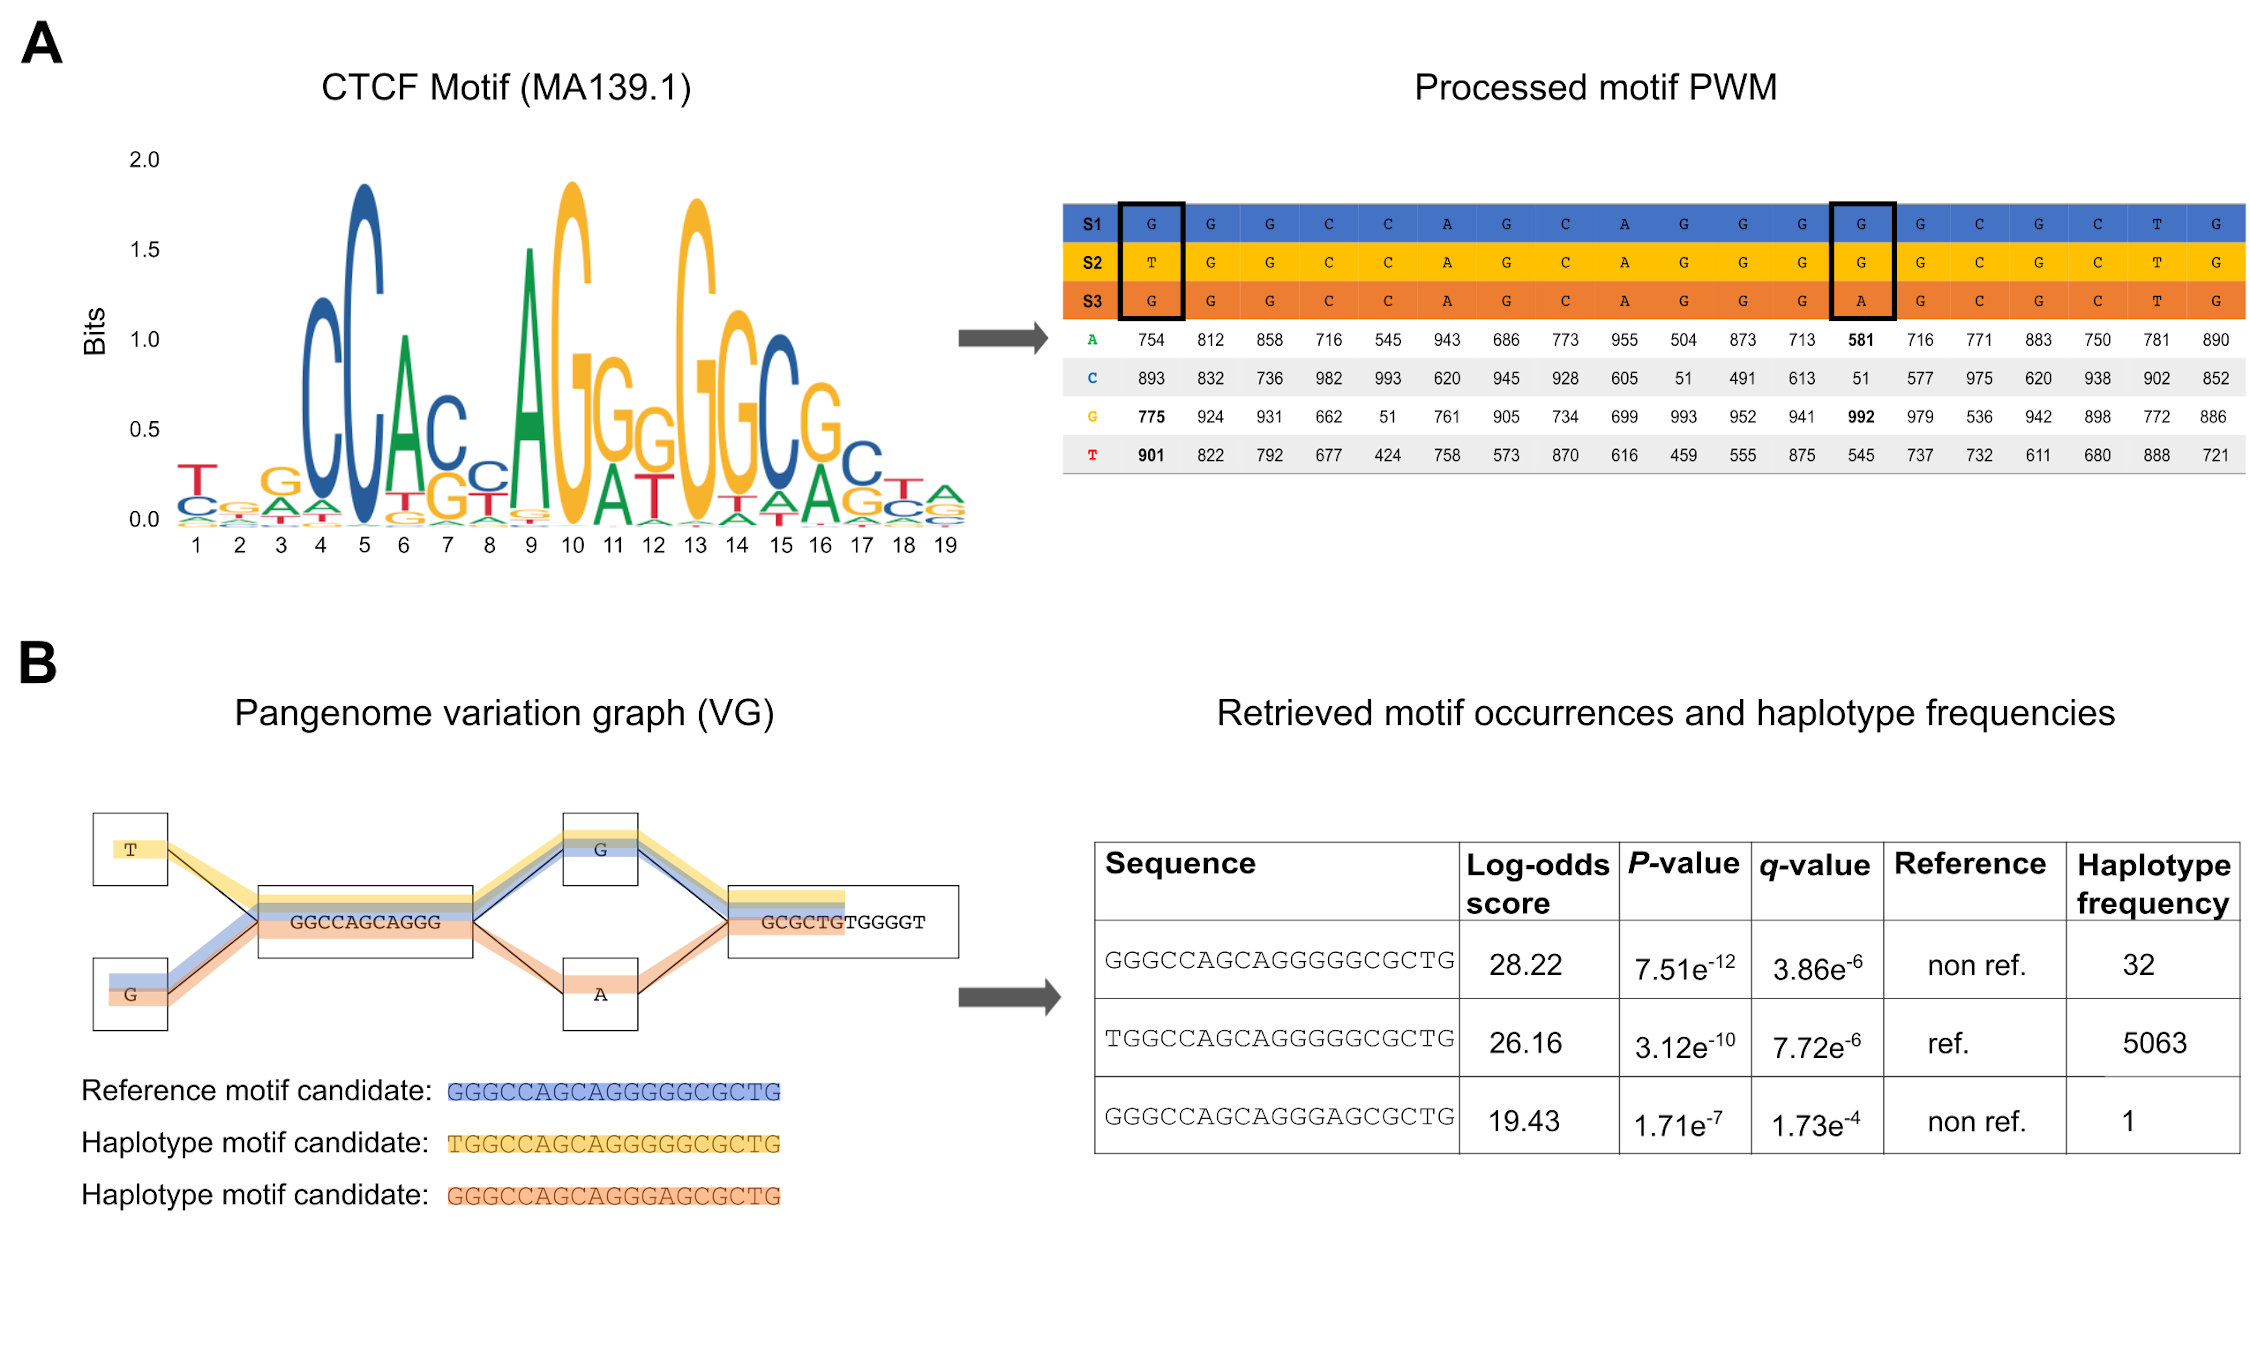
\includegraphics[width=\textwidth]{figures/grafimo1.png}
	\caption[\grafimo TF motif search workflow.]{\textbf{\grafimo TF motif search workflow. (A)} The motif PWM (in MEME or JASPAR format) is processed and its values are scaled in the range [0, 1000]. The resulting score matrix is used to assign a score and a corresponding P-value to each motif occurrence candidate. In the final report \grafimo returns the corresponding log-odds scores, which are retrieved from the scaled values. \textbf{(B)} \grafimo slides a window of length k, where k is the motif width, along the haplotypes (paths in the graph) of the genomes used to build the VG. The resulting sequences are scored using the motif scoring matrix and are statistically tested assigning them the corresponding P-value and q-value. Moreover, for each entry is assigned a flag value stating if it belongs to the reference genome sequence ("ref") or contains genomic variants ("non.ref") and is computed the number of haplotypes in which the sequence appears.}
	\label{fig:grafimo1}
\end{figure} 

% --- Processing of Position Weight Matrix to Position Specific Scoring Matrix
\subsubsection{Processing of Position Weight Matrix to Position Specific Scoring Matrix}
\grafimo utilizes Position Specific Scoring Matrices (PSSMs) to assign scores to potential motif occurrences. These PSSMs are generated through the processing of input PWMs provided in JASPAR (\textbf{Appendix \ref{section:jaspar-format}}) or MEME (\textbf{Appendix \ref{section:meme-format}}) format. Let us assume the input motif PWM $M$ is provided in JASPAR format and $|M| = m$, then \grafimo starts by deriving the corresponding position probability matrix $M_{p}$:
\[
    M_{p} = \frac{M[n,i]}{\sum_{n \in \Sigma}{M[n,i]}}
\]
where $\Sigma=\{A,C,G,T\}$ and $1 \leq i \leq m$. On the other hand, if the input binding site is provided in MEME format, \grafimo skips this step since the motif is already represented as a probability matrix. After computing $M_{p}$, \grafimo normalizes each probability returning a normalized position probability matrix $M_{p}'$:
\[
    M_{p}' = \frac{M_{p}[n,i]}{\sum_{n \in \Sigma}{M_{p}[n,i]}}
\]
where $\Sigma=\{A,C,G,T\}$ and $1 \leq i \leq m$. To account for the frequency of emission of each symbol in the alphabet $\Sigma=\{A,C,G,T\}$ (genomic frequency of each nucleotide), users can provide \grafimo with a 0-th order background model $B$. In the absence of a user-defined background distribution, \grafimo assumes a uniform distribution. To prevent divisions by zero in subsequent processing steps and accommodate the potential lack of information, each normalized probability in $M_{p}'$ is incremented by a pseudocount. Typically, pseudocounts are small values, ranging between 0.1 and $1\text{e}^{-4}$. Next, each value in $M_{p}'$ is adjusted by adding the pseudocount and weighting the resulting values with the background model probability distribution:
\[
    M_{p}'' = \frac{M_{p}'[n,i] \cdot \sum_{n \in \Sigma}{M[n,i] + p \cdot B_{n}}}{\sum_{n \in \Sigma}{M[n,i] + p}}
\]
where $\Sigma=\{A,C,G,T\}$ and $1 \leq i \leq m$. Following these steps, the probabilities are transformed into log-likelihood scores, often referred to as \emph{log-odds}. Each value in $M_{p}''$, undergoes this transformation to obtain the final PSSM:
\[
    \text{PSSM}[n,i] = \log_{2}{\left (\frac{M_{p}''[n,i]}{B_{n}} \right )}
\]
The resulting PSSM is then utilized to calculate a log-likelihood or binding affinity score for each candidate motif occurrence.

% --- Evaluating motif statistical significance
\subsubsection{Evaluating motif statistical significance via dynamic programming}
To evaluate the significance of the score assigned to a candidate binding site occurrence, is essential to consider the likelihood of such a log-odds value occurring by chance. This probability can be estimated by establishing a null hypothesis model, representing the random occurrence of $m$ nucleotides matching the motif. Recall that $|M|=m$, where $M$ is the input motif. A na\"ive approach to derive a null model involves randomly shuffling nucleotides $n \in \Sigma$, obtaining random sequences $s$, where $|s|=m$, and score each $s$ using the PSSM. The resulting scores under this null model would be purely chance-driven. The probability that a score, obtained under the null hypothesis, is at least as large as the one observed in the real model is defined $P$-value in motif scanning context \citep{noble2009does}. Essentially, the $P$-value for an observed score represents the area under the score $\text{score}(s)$ distribution obtained after the random shuffle of nucleotides, where $x \geq \text{score}(s)$. Although shuffling nucleotides to obtain would result in accurate $P$-values, this procedure is not computationally feasible. To tackle this challenge efficiently, \grafimo implements a dynamic programming (DP) algorithm \citep{griffin1994staden}. This algorithm assumes that the scored sequence is randomly generated with a specified frequency associated to each nucleotide. To facilitate the implementation of the DP-algorithm, \grafimo scales the values stored in the log-odds matrix PSSM, ensuring they fall within the range $0 \leq \text{PSSM}(n,i) \leq 1000$:
\[
    \text{PSSM}_{\text{scaled}}[n,i] = \left \lfloor \left ( \text{PSSM}[n,i] - \lfloor \min{\text{PSSM}} \rfloor \cdot \left \lfloor \frac{1000}{\max{\text{PSSM}}-\min{\text{PSSM}}} \right \rfloor \right ) \right \rceil
\]
where $\Sigma=\{A,C,G,T\}$ and $1 \leq i \leq m$. The result is a new matrix $\text{PSSM}_{\text{scaled}}$ with integer values ranging from 0 to 1000. Using integers instead of floatong-point values, enables fast computations. Subsequently, a null model distribution is computed for each sequence $s_{r}$ randomly obtained, with $1 \leq |s_{r}| \leq m$. This is done following the probabilities defined in the background distribution $B$. A $m \times (1000 \cdot m + 1)$ matrix $P$ is built, with entries filled using \textbf{Algorithm \ref{alg:grafimo-dp-nullmodel}}. The rows of $P$ represent sequences length, while columns represent a score that can be obtained for a motif occurrence using $\text{PSSM}_{\text{scaled}}$. At the end of the procedure, each entry $P[i,j]$ contains the number of sequences $|S_{r}|$, where $|s_{r}| = i$ and $\text{score}(s_{r})=j$, for each $s_{r} \in S_{r}$ with a score j. Sequences $s_{r}$, represent randomly generated strings following the background distribution. The time complexity of this algorithm is $O(n \cdot m)$, where $n$ is the number of rows and $m$ is the number of columns of $P$. The space needed by the algorithm is $O(n)$, as once the current row is completely computed, the preceding one is removed and is no longer needed in subsequent steps of the algorithm.

% - algorithm: Dynamic programming algorithm computing null model in GRAFIMO (Griffin et al., 1994)
\begin{algorithm}[!]
    \caption{Dynamic programming algorithm computing null model in \grafimo \citep{griffin1994staden}}
    \label{alg:grafimo-dp-nullmodel}
    \KwData{$\text{PSSM}_{\text{scaled}}$, $M$, $B$, $\Sigma$}
    \KwResult{$P$}
    $m \gets |M|$ \Comment*[r]{$M$ is the input motif}
    $c \gets 1000 \cdot m + 1$\;
    \For{\text{$i$ \textbf{in} $1$ \textbf{to} $m$}}{
        \For{$n \in \Sigma$}{
            \If{$i=0$}{
                $P[0,M[n,i]] \gets P[0,M[n,i]] + 1 \cdot B_{n}$\;
            }
            \Else{
                \For{\text{$j$ \textbf{in} $1$ \textbf{to} $c$}}{
                    \If{$P[i-1,j] \neq 0$}{
                        $P[i,M[n,i]+j] \gets P[i,M[n,i]+j] + P[i-1,j] \cdot B_{n}$\;
                    }
                }
            }
        }    
    }
    \Return{$P$}
\end{algorithm}

% --- Searching motif occurrences on genome graphs
\subsubsection{Searching motif occurrences on genome graphs}
After computing the PSSM and its corresponding $P$-value matrix $P$ from the input motif $M$, \grafimo begins a scanning process across the input genome graph within the input genomic regions (\textbf{Algorithm \ref{alg:grafimo-motif-scanning}}). The traversal of graph nodes is achieved performing a Breadth-First Search (BFS)-like algorithm operating in parallel. The scanning progresses by employing a sliding window of width $m$, where $|M|=m$. While scanning the graph, \grafimo recover all consecutive overlapping segments of length $m$. When a node with two or more outgoing edges is encountered, indicating the presence of one or more alternative alleles at that position, \grafimo visits only the haplotypes belonging to the allowed paths in the graph. Subsequently, each sequence extracted from the genome graph is scored using the PSSM (\textbf{Algorithm \ref{alg:grafimo-sequence-score}}). The score for each sequence $s$ is the sum of the values of entries $\text{PSSM}_{\text{scaled}}[n,i]$, where $n=s_{i}$ and $1 \leq i \leq m$. To speed-up the score computation, \grafimo utilizes the PSSM with scaled values instead of the one with log-likelihood scores, as operations on integers are faster than those on floating-point values. The resulting score for each sequence $\text{score}(s)$ is then transformed back into a log-likelihood score $LL(s)$:
\[
    LL(s) = \left ( \frac{\text{score}(s)}{1000 / \max{\text{PSSM}} - \min{\text{PSSM}}} \right ) + m \cdot \lfloor \min{\text{PSSM}} \rfloor
\]
The complexity of the scoring procedure is $O(n \cdot m)$, where $n$ is the total number of sequences to score, and $m$ is their length. In scenarios where numerous scores are reported, such as scanning a genome for TFBS motif occurrences, relying solely on a $P$-value is insufficient to assess statistical significance. In fact, $P$-values are statistically valid only when computing a single score \citep{noble2009does}. To address this limitation, \grafimo corrects $P$-values for multiple hypothesis tests using false discovery rate estimation (FDR), providing a corresponding $q$-value. FDRs are computed directly from $P$-values using the Benjamini-Hochberg procedure.

% - algorithm: GRAFIMO motif scanning algorithm
\begin{algorithm}[!]
    \caption{\grafimo motif scanning algorithm}
    \label{alg:grafimo-motif-scanning}
    \KwData{$G$, $M$}
    \KwResult{$\text{scores}$, $\text{pvalues}$}
    $\text{PSSM} \gets \text{computePSSM}(M)$ \Comment*[r]{see previouse sections for details}
    $P \gets \text{computePvalueMatrix}(\text{PSSM})$ \Comment*[r]{see Algorithm \ref{alg:grafimo-dp-nullmodel} for details}
    $S \gets \text{recoverSequencesBFS}(G)$ \Comment*[r]{each $s \in S$ satisfies $|s|=|M|$}
    $\text{scores} \gets \emptyset$\;
    $\text{pvalues} \gets \emptyset$\;
    \For{$s \in S$}{
        $\text{score}(s), \text{pvalue}(s) \gets \text{computeScorePvalue}(s, \text{PSSM}, P)$ \Comment*[r]{details in Algorithm \ref{alg:grafimo-sequence-score} }
        $\text{scores}[i] \gets \text{score}(s)$\;
        $\text{pvalues}[i] \gets \text{pvalue}(s)$\; 
    }
    \Return{$\text{scores}$, $\text{pvalues}$}
\end{algorithm}

% - algorithm: Compute sequence score and P-value
\begin{algorithm}[!]
    \caption{Compute sequence score and $P$-value}
    \label{alg:grafimo-sequence-score}
    \KwData{$s$, $\text{PSSM}$, $P$}
    \KwResult{$\text{score}$, $\text{pvalue}$}
    $\Sigma \gets \{A,C,G,T\}$\;
    $\text{score} \gets 0$\;
    \For{$i$ \textbf{in} $1$ \textbf{to} $|s|$}{
        $n \gets s(i)$\;
        \If{$n \notin \Sigma$}{
            $\text{score} \gets 0$ \Comment*[r]{The sequence contains N, assign the lowest possible score} 
            $\text{\textbf{break}}$\;
        }
        $\text{score} \gets \text{score} + \text{PSSM}(n,i)$\;
    }
    $\text{pvalue} \gets \sum^{|P|}_{j=\text{score}}{\frac{P(j)}{\sum^{|P|}_{k=1}{P(k)}}}$\;
    \Return{$\text{score}$, $\text{pvalue}$}
\end{algorithm}

% ---- Report generation
\subsection{Report generation}
\grafimo interface has been designed with inspiration drawn from FIMO, allowing seamless integration into pipelines and workflows originally built on FIMO. Similar to FIMO, \grafimo generates three distinct reports: a tab-delimited file (TSV), an HTML report, and a GFF3 file compatible with the UCSC Genome Browser \citep{lee2020ucsc}. The TSV report (\textbf{Fig.\ref{fig:grafimo-tsv}}) lists each found candidate TFBS along with its score, genomic location (start, stop, and strand), and statistical significance ($P$-value and $q$-value). Moreover, it reports the number of haplotypes in which each motif candidate has been observed, with a flag value highlighting whether the occurrence was found only on alternative haplotypes or also in the reference sequence. \grafimo also provides an HTML version of the TSV report (\textbf{Fig.\ref{fig:grafimo-html}}), that can be easily explored with any web browser. The GFF3 report is compatible with the UCSC Genome Browser, allowing users to load it as a custom track (\textbf{Fig.\ref{fig:grafimo-genome-browser}}). This enables the visualization and exploration of the identified TFBS candidates alongside additional annotations available in the Genome Browser, such as nearby genes, enhancers, promoters, or pathogenic variants sourced from the ClinVar database \citep{landrum2020clinvar}.

% - figure: GRAFIMO TSV summary report
\begin{figure}[!]
    \centering
    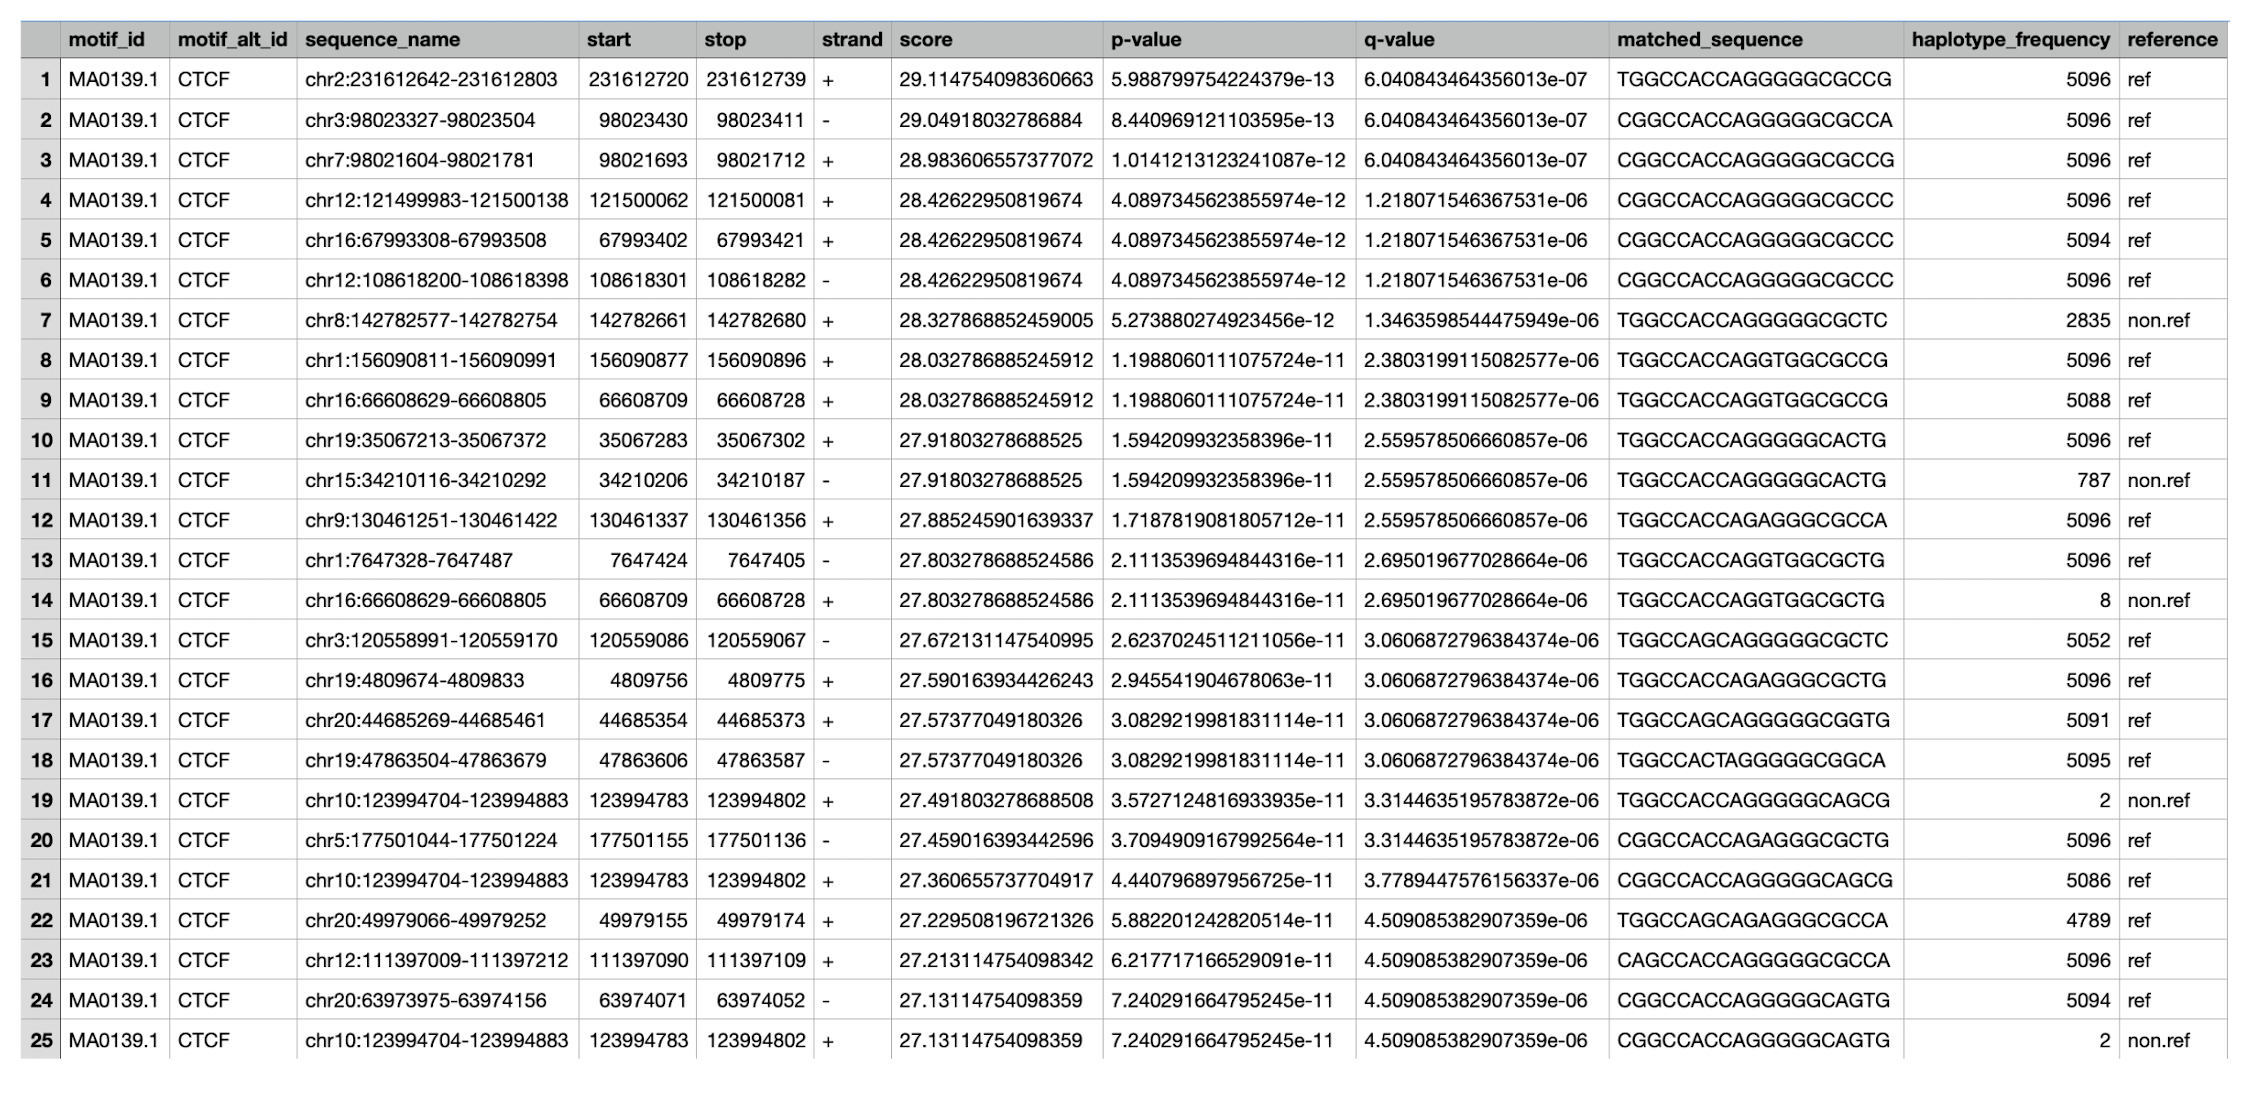
\includegraphics[width=\textwidth]{figures/grafimo-tsv-report.png}
    \caption[\grafimo TSV summary report]{\textbf{\grafimo TSV summary report.} The tab-delimited report shows the first 25 potential CTCF occurrences retrieved by \grafimo, searching CTCF motif in ChIP-seq peak regions on A549 cell line (ENCODE experiment ENCFF816XLT).}
    \label{fig:grafimo-tsv}
\end{figure}

% - figure: GRAFIMO HTML summary report
\begin{figure}[!]
    \centering
    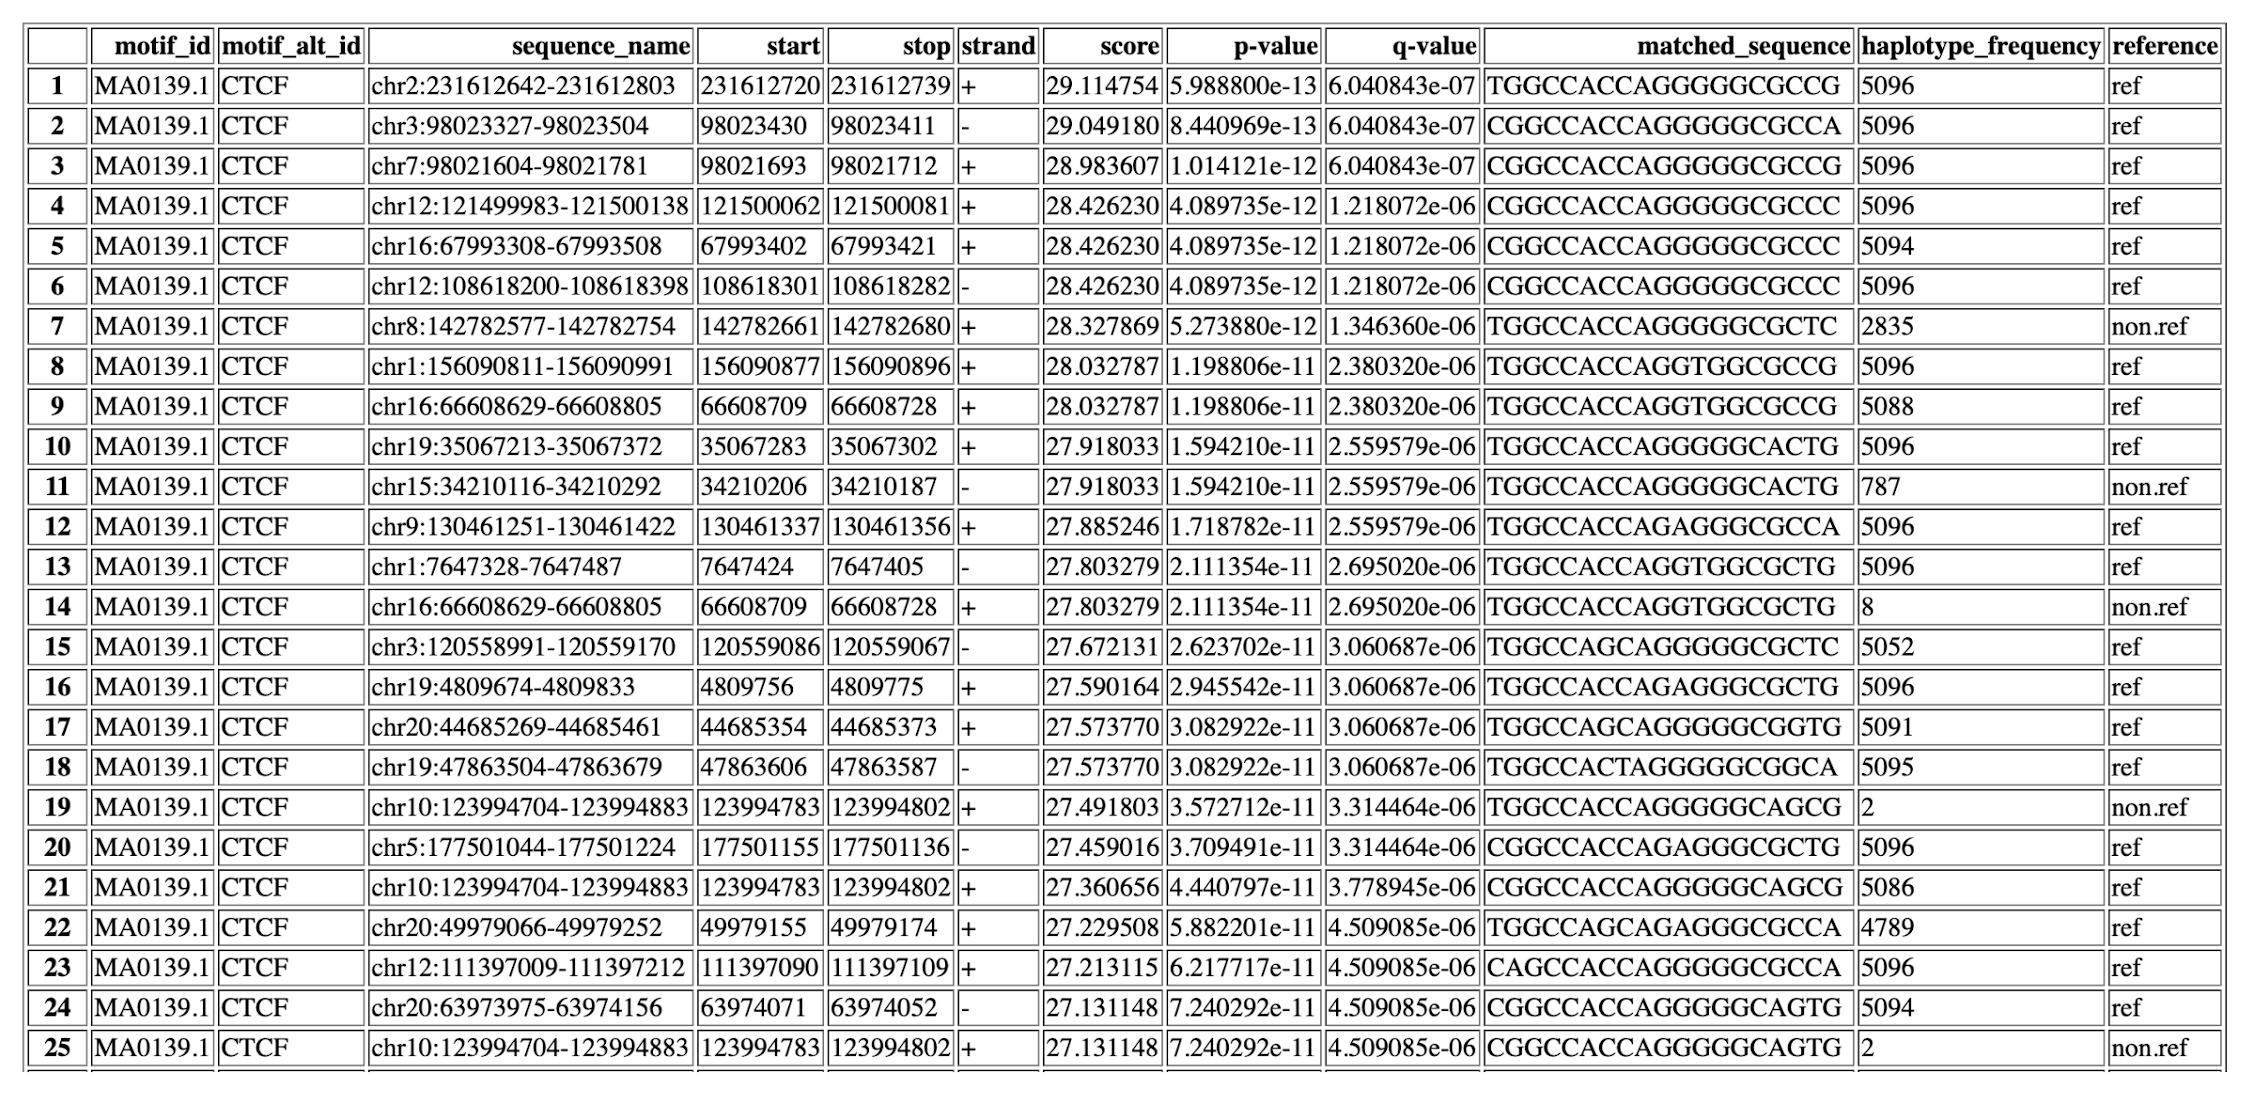
\includegraphics[width=\textwidth]{figures/grafimo-html.png}
    \caption[\grafimo HTML summary report]{\textbf{\grafimo HTML summary report.} The HTML report displays the first 25 potential CTCF occurrences retrieved by searching CTCF motif occurrences with \grafimo on ChIP-seq regions on A549 cell line (ENCODE experiment ENCFF816XLT).}
    \label{fig:grafimo-html}
\end{figure}

% - figure: GFF3 track returned by GRAFIMO and loaded on the UCSC Genome Browser 
\begin{figure}[!]
    \centering
    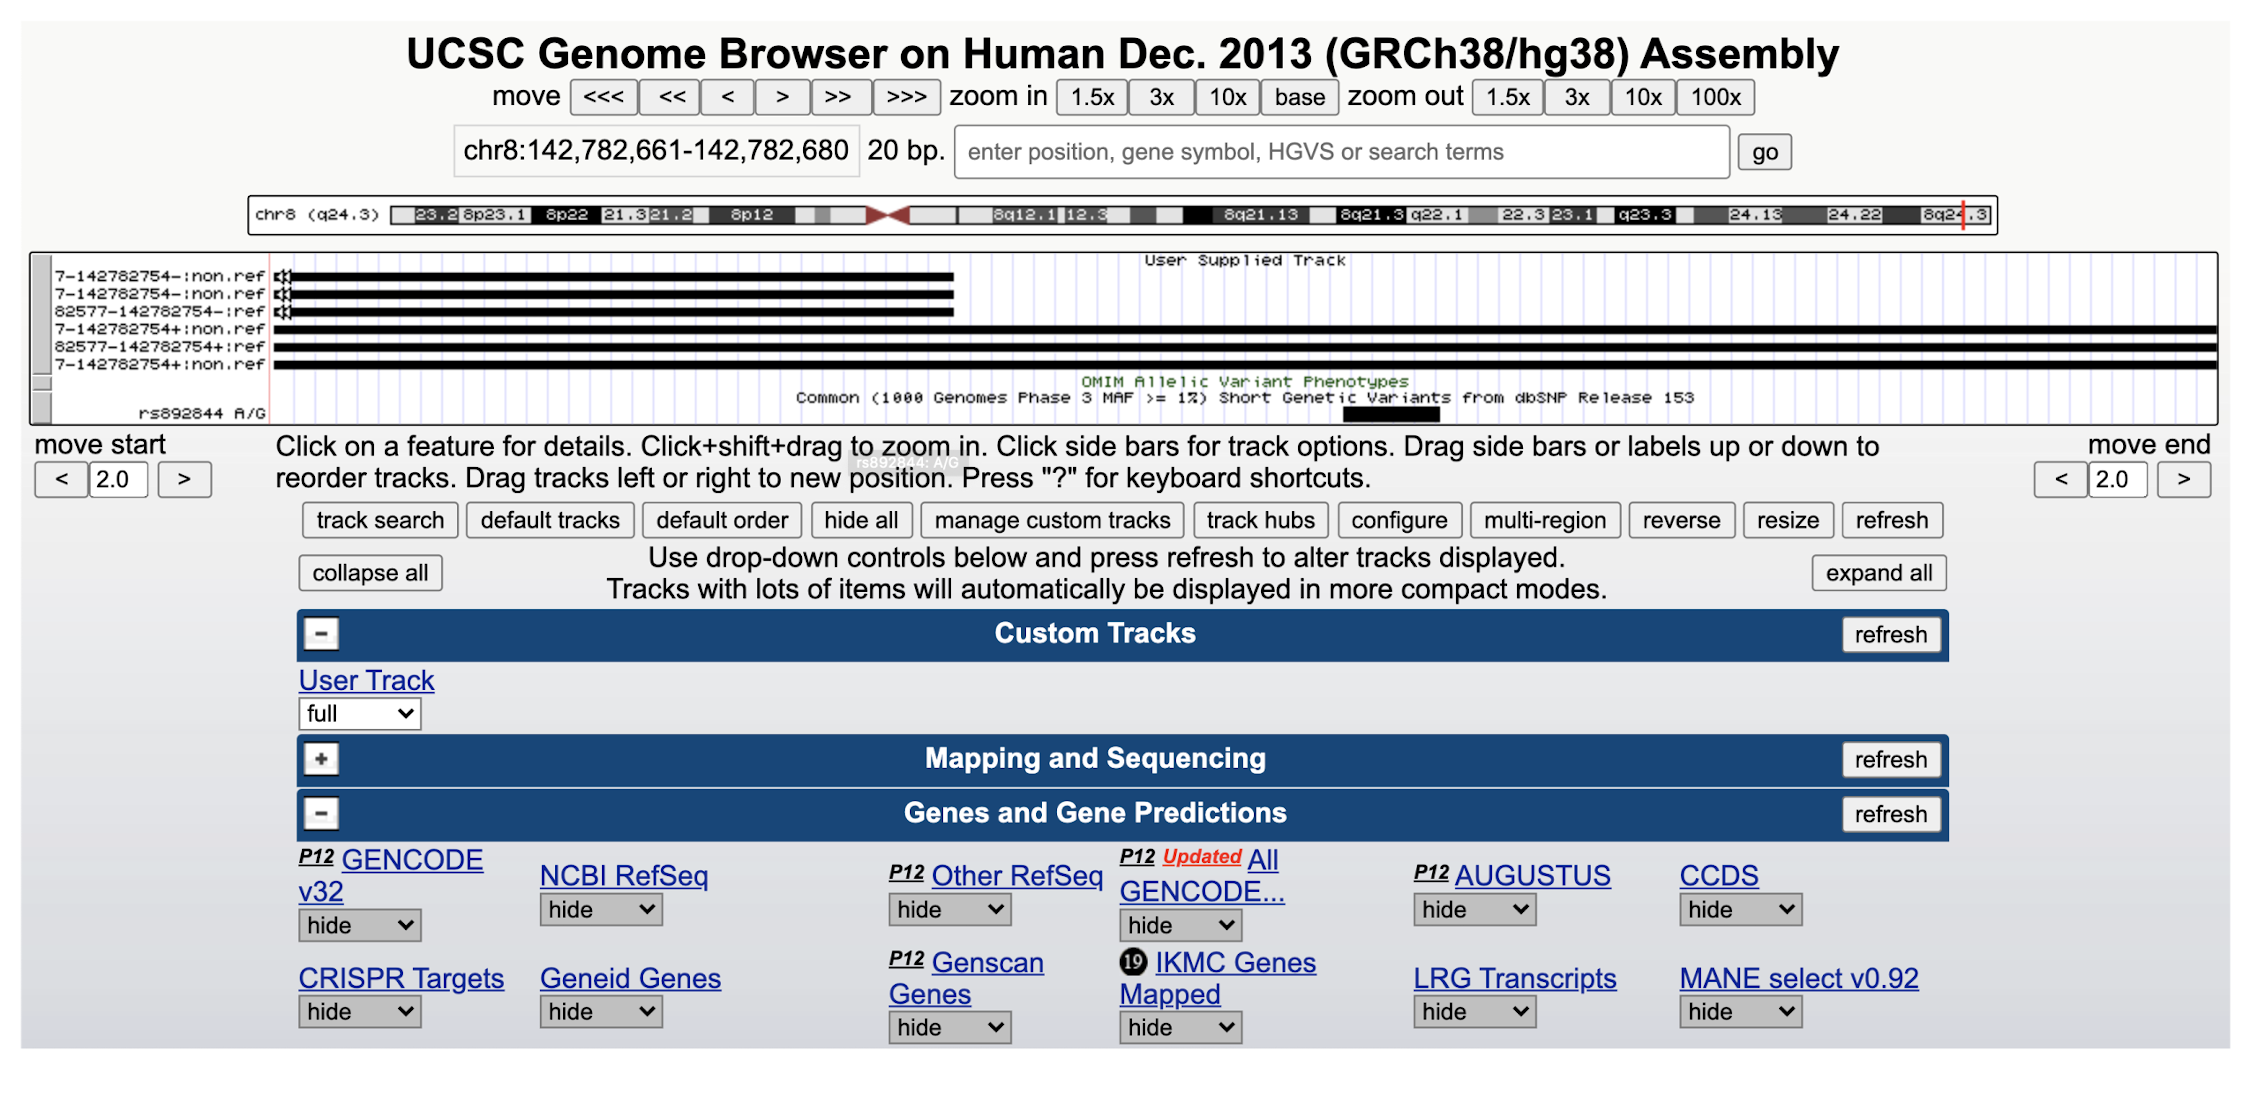
\includegraphics[width=\textwidth]{figures/grafimo-genome-browser.png}
    \caption[GFF3 track returned by \grafimo and loaded on the UCSC Genome Browser]{\textbf{GFF3 track returned by GRAFIMO and loaded on the UCSC Genome Browser.} \grafimo produces a GFF3 report which can be loaded on the UCSC Genome Browser. The custom track loaded in the example shows three potential CTCF occurrences (region chr8:142,782,661-142,782,680) recovered by \grafimo, which overlap a dbSNP annotated variant (rs892844).}
    \label{fig:grafimo-genome-browser}
\end{figure}

% ----- Searching motif occurrences with GRAFIMO
\section{Searching motif occurrences with \grafimo}
\grafimo's main aim is to investigate the potential impact of genetic variants on the binding affinity of putative TFBS across a set of individuals. By leveraging genome graphs, \grafimo may recover additional sites that might be missed when considering linear reference genomes exclusively, without accounting for genetic variants. To showcase its utility, we constructed a genome graph based on 2,548 individuals from 1KGP phase 3 (hg38 human genome assembly) \citep{zheng2017alignment, lowy2019variant}. The resulting graph encoded their genetic variants ($\sim$78 millions, SNPs and indels (\textbf{Table \ref{table-1KGP-variants}})) and phased haplotypes (total of 5,096 haplotypes). Subsequently, we searched the graph for putative TFBS of three TF motifs retrieved from the JASPAR database \citep{sandelin2004jaspar, fornes2020jaspar}: CTCF (JASPAR ID MA0139.1), ATF3 (JASPAR ID MA0605.2), and GATA1 (JASPAR ID MA0035.4) (\textbf{Fig.\ref{fig:grafimo-motifs}}). The three motifs exhibit diversity in length (from 11 to 19 bp), information content, and evolutionary conservation. To investigate regions with likely true binding events, we focused our analysis on ChIP-seq peak regions in six different cell lines (A549, GM12878, H1, HepG2, K562, MCF-7) retrieved from the ENCODE Project database \citep{encode2012integrated, davis2018encyclopedia} (\textbf{Table \ref{tab:table-encode-experiment}}). 
%
% - figure: Transcription factor motifs used to test GRAFIMO
\begin{figure}[!]
    \centering
    \includegraphics[width=\textwidth]{figures/grafimo-motifs.png}
    \caption[Transcription factor motifs used to test \grafimo]{\textbf{Transcription factor motifs used to test \grafimo.} Transcription factor binding site motifs of \textbf{(A)} CTCF, \textbf{(B)} ATF3, and \textbf{(C)} GATA1.}
    \label{fig:grafimo-motifs}
\end{figure}
%
% - table: Genetic variants in the 1KGP genome graphs
\begin{table}[!]
    \centering
    \begin{tabular}{|p{4cm}|p{6cm}|}
        \hline
        \textbf{Chromosome} & \textbf{Number of genetic variants} \\
        \hline
        Chr1 & 6,191,833\\
        \hline
        Chr2 & 6,790,551\\
        \hline
        Chr3 & 5,641,493\\
        \hline
        Chr4 & 5,477,810\\
        \hline
        Chr5 & 5,115,036\\
        \hline
        Chr6 & 4,863,337\\
        \hline
        Chr7 & 4,511,408\\
        \hline
        Chr8 & 4,425,449\\
        \hline
        Chr9 & 3,384,360\\
        \hline
        Chr10 & 3,874,259\\
        \hline
        Chr11 & 3,881,791\\
        \hline
        Chr12 & 3,745,465\\
        \hline
        Chr13 & 2,760,845\\
        \hline
        Chr14 & 2,548,903\\
        \hline
        Chr15 & 2,301,453\\
        \hline
        Chr16 & 2,548,920\\
        \hline
        Chr17 & 2,209,149\\
        \hline
        Chr18 & 2,189,529\\
        \hline
        Chr19 & 1,738,824\\
        \hline
        Chr20 & 1,817,492\\
        \hline
        Chr21 & 1,045,269\\
        \hline
        Chr22 & 1,059,079\\
        \hline
        ChrX & 106,963\\
        \hline
    \end{tabular}
    \caption[Genetic variants in the 1KGP genome graphs]{\textbf{Genetic variants in the 1KGP genome graphs.} Number of genetic variants (SNPs and indels) in the genome graph constructed using 1KGP phase 3 on hg38 data. The variants belong to 2,548 individuals from 26 populations. In total the genome graphs encoded $\sim$78 millions variants\\ \hfill.}
    \label{table-1KGP-variants}
\end{table}
%
% - table: ENCODE ChIP-seq experiment codes
\begin{table}[!]
    \centering
    \resizebox{\columnwidth}{!}{%
    \begin{tabular}{|l|l|l|l|l|l|l|}
        \hline
        \textbf{Motif} & \textbf{A549} & \textbf{GM12878} & \textbf{H1} & \textbf{HepG2} & \textbf{K562} & \textbf{MCF-7} \\ \hline
        CTCF  & ENCFF816XLT & ENCFF267NYF &             & ENCFF015OJG & ENCFF895HAG                                                       & ENCFF088JWU \\ \hline
        ATF3  &             &             & ENCFF207AVV & ENCFF753WNT & ENCFF787GVU                                                       &             \\ \hline
        GATA1 &             &             &             &             & \begin{tabular}[c]{@{}l@{}}ENCFF811YFQ\\ ENCFF939ODZ\end{tabular} &             \\ \hline
    \end{tabular}%
    }
    \caption[ENCODE ChIP-seq experiments]{\textbf{ENCODE ChIP-seq experiments.} To test our software we searched potential occurrences of three transcription factor motifs (CTCF, ATF3, and GATA1) in a hg38 genome graph enriched with genetic variants and haplotypes of 2,548 individuals from 1000 Genomes Project phase 3.}
    \label{tab:table-encode-experiment}
\end{table}
%
For each TF, we systematically acquired the optimal IDR thresholded peaks from ENCODE (bigBED format). Subsequently, we employed UCSC's \texttt{bigBedToBed} tool \citep{kent2010bigwig} to convert each bigBED file into its corresponding BED. To enhance data quality, we filtered the resulting BED files, excluding features mapped to non-canonical chromosomes. The filtered BEDs were then subjected to sorting based on both $q$-values and peak signals. This sorting allowed us to prioritize the identification of the most informative regions, specifically selecting the top 3,000 peaks for each experiment. Then, we performed a comprehensive scan on the prioritized regions using \grafimo. In our subsequent downstream analyses, we retained those sites that exhibited a $P$-value $< 1e^{-4}$. This stringent threshold ensured a focus on statistically significant potential motif occurrences. Finally, we considered the sites meeting these criteria as potential binding sites for the respective TFs under investigation. Based on the retrieved sites, we consistently observed across the three investigated TFs that genetic variants can significantly affect the estimated binding affinity. 

% ---- Searching for CTCF occurrences
\subsection{Searching for CTCF occurrences}
% - figure: Searching CTCF motif on genome graphs using GRAFIMO provides insights on the impact of genetic diversity on putative binding sites
\begin{figure}
    \centering
    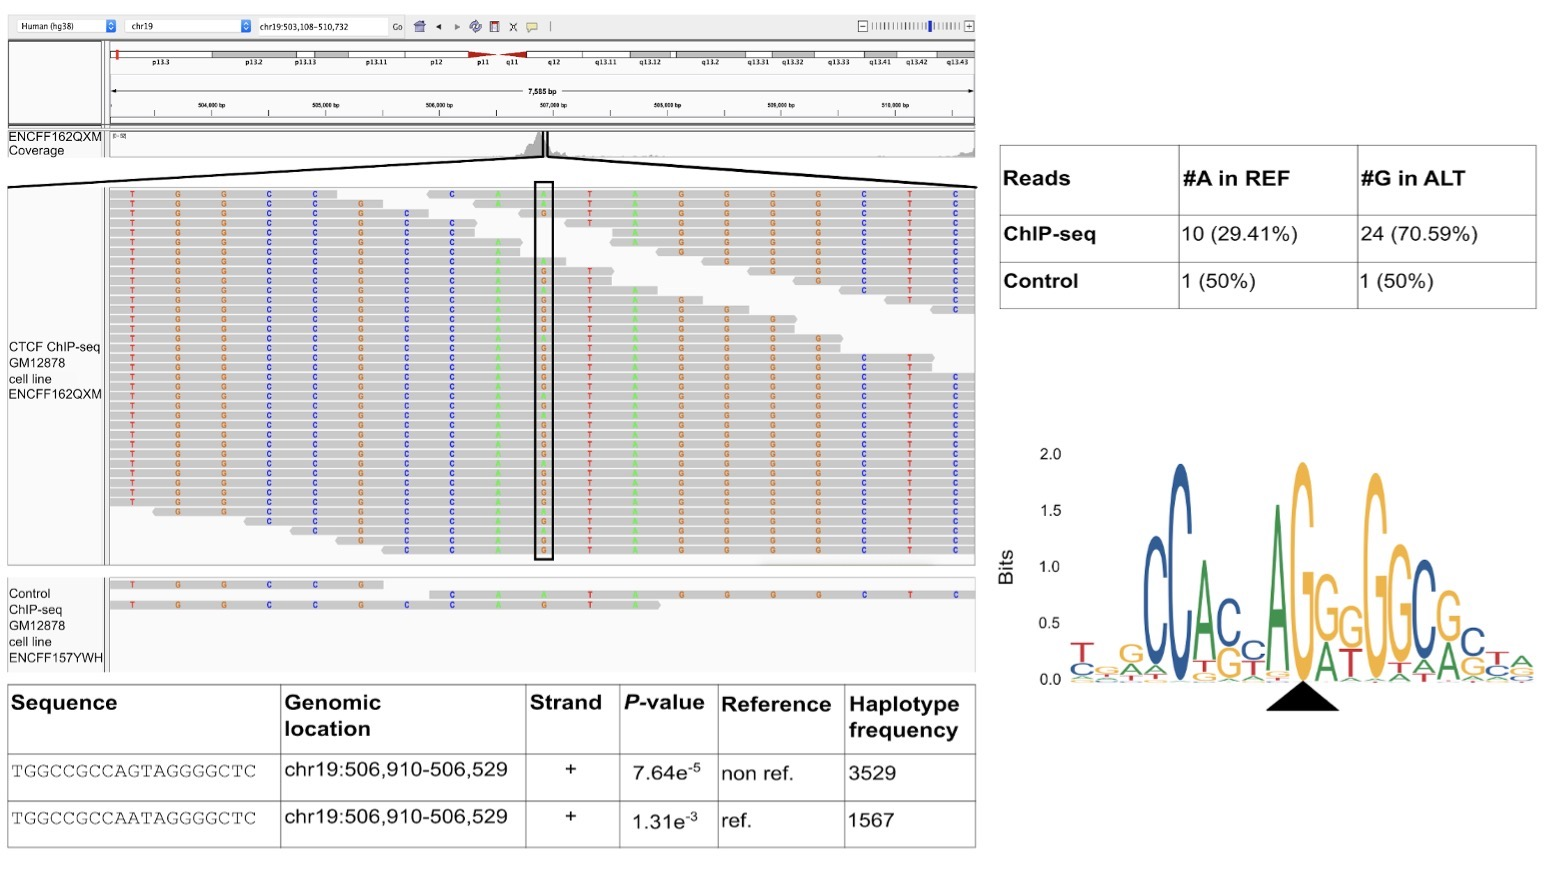
\includegraphics[width=\textwidth]{figures/grafimo2.jpg}
    \caption[Searching CTCF motif on genome graphs using \grafimo provides insights on the impact of genetic diversity on putative binding sites]{\textbf{Searching CTCF motif on genome graphs using \grafimo provides insights on the impact of genetic diversity on putative binding sites. (A)} Statistically significant ($P$-value $< 1e^{-4}$) and non-significant potential CTCF occurrences found in the reference and haplotype sequences found using \grafimo on 1KGP genome graph. \textbf{(B)} Statistical significance of the identified CTCF occurrences and their frequency within the haplotypes embedded in the genome graph. \textbf{(C)} Percentage of statistically significant potential CTCF binding sites found only in the reference genome, only in alternative haplotypes, and with their binding scores modulated by 1KGP genetic variants. \textbf{(D)} Percentage of population-specific and common (shared by two or more populations) CTCF binding sites found in individual haplotypes.}
    \label{fig:grafimo-ctcf}
\end{figure}
% 
CTCF is a zinc-finger transcription factor involved in transcriptional regulation, playing a pivotal role in epigenetic control \citep{ishihara2006ctcf}, and functioning as a tumor suppressor \citep{fiorentino2012tumor}. In our experiments, we performed a targeted search for CTCF motif (JASPAR ID MA0139.1) (\textbf{Fig.\ref{fig:grafimo-motifs} (A)}) occurrences within the 1KGP genome graph. Interestingly, we found a substantial number of CTCF motif occurrences exclusive to non-reference haplotypes, indicating that a significant pool of potential TFBS is overlooked when scanning the genome without considering genetic variants (\textbf{Fig.\ref{fig:grafimo-ctcf} (A)}). Furthermore, our analysis identified several highly significant CTCF occurrences within rare haplotypes (\textbf{Fig.\ref{fig:grafimo-ctcf} (B)}), that may influence gene expression in individuals showing these haplotypes. We investigated the genomic locations of significant motif occurrences to assess how individual binding sites might be affected by genetic diversity--whether disrupted, created, or modulated. Interestingly, our experiments revealed that 6.13\% of potential CTCF binding sites were exclusive to non-reference haplotypes, 5.94\% were disrupted by variants in non-reference haplotypes, and approximately 30\% retained significance in non-reference haplotypes, but with different binding scores (\textbf{Fig.\ref{fig:grafimo-ctcf} (C)}). Notably, a considerable portion of putative binding sites recovered solely on individual haplotypes exhibited population specificity. For instance, 24.66\%, 6.74\%, 5.68\%, 13.01\%, and 12.52\% of potential CTCF binding sites retrieved exclusively from individual haplotypes were specific to AFR, EUR, AMR, SAS, and EAS populations, respectively (\textbf{Fig.\ref{fig:grafimo-ctcf} (D)}). Among the unique motif occurrences identified exclusively in non-reference haplotypes in CTCF ChIP-seq peaks, we uncovered a TFBS (chr19:506,910-506,929) that illustrates the pitfalls of relying solely on reference genomes for motif scanning. In this genomic locus, we identified a heterozygous SNP aligning with position 10 of the CTCF matrix, that significantly modulates the binding affinity of the corresponding binding site. By inspecting ChIP-seq reads (experiment ENCSR000DZN on GM12878), an allelic imbalance emerged towards the alternative allele. The alternative allele G exhibited a clear prevalence (70.59\% of reads), while the reference allele A lagged behind at 29.41\% of reads. This allelic imbalance is not observed in the control reads (experiment ENCSR000EYX) (\textbf{Fig.\ref{fig:grafimo-allelic-imbalance}}).
% 
% - figure: Considering genomic diversity, GRAFIMO captures additional binding events
\begin{figure}
    \centering
    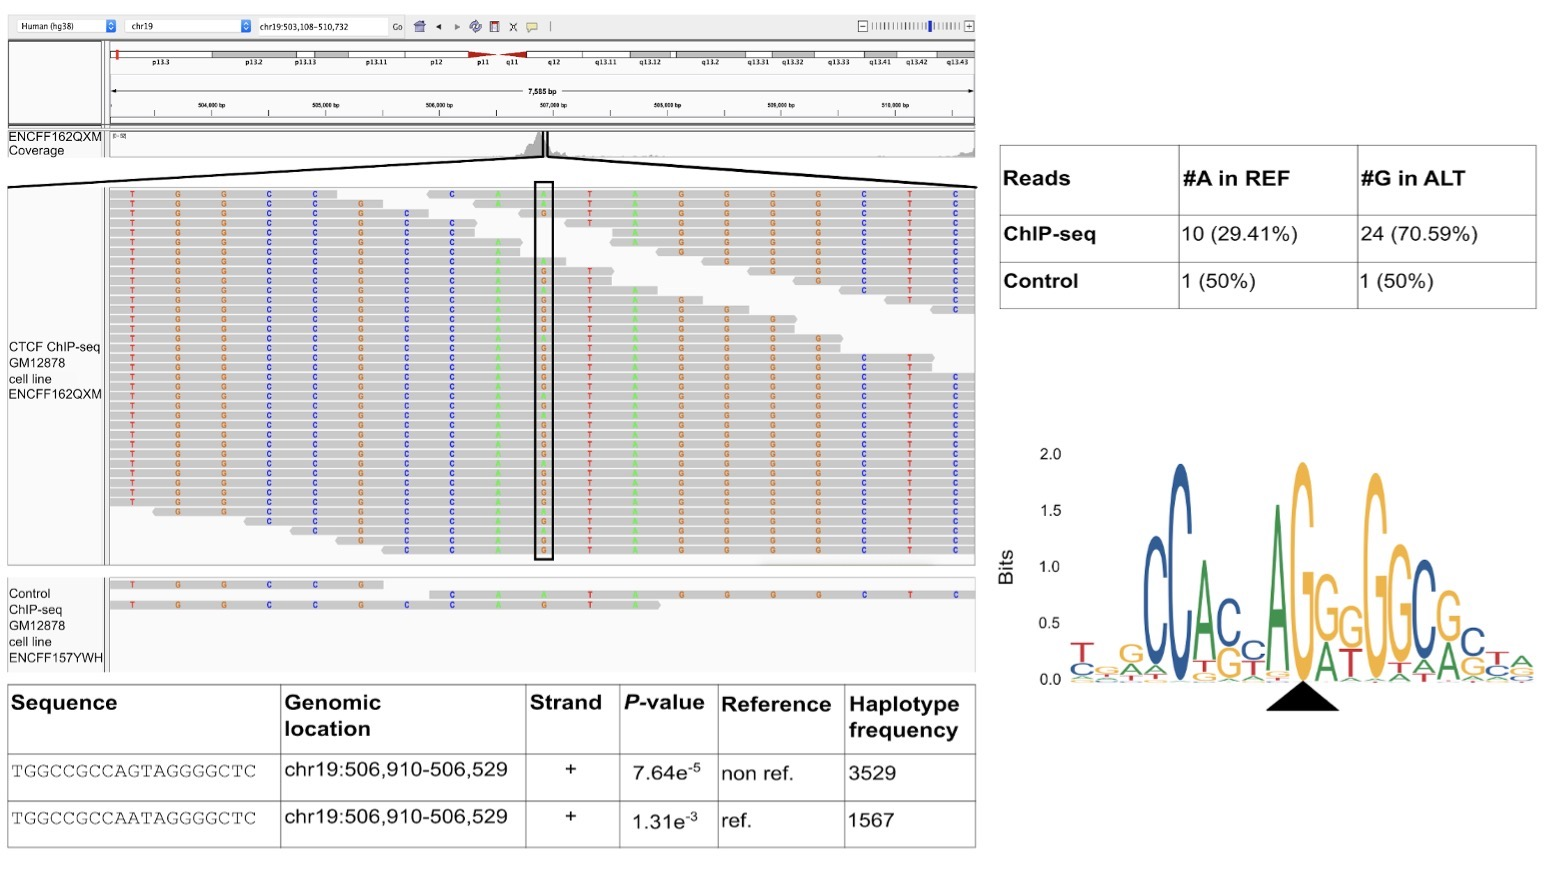
\includegraphics[width=\textwidth]{figures/grafimo3.jpg}
    \caption[Considering genomic diversity, \grafimo captures additional binding events]{\textbf{Considering genomic diversity, \grafimo captures additional binding events.} \grafimo reports a potential CTCF binding site at chr19:506,910-506,929 exclusively present in haplotype sequences. The binding site was identified by scanning CTCF ChIP-seq peaks (experiment ENCSR000DZN on GM12878). The analysis of ChIP-seq reads (ENCFF162QXM) unveils an allelic imbalance at position 10 of the motif, towards the alternative allele (G). \grafimo accurately captures this imbalance by reporting sequences carrying a G at position 10 (as found in the alternative haplotypes), while the potential TFBS on the reference, which carries an A, is not reported as statistically significant. This discrepancy aligns with CTCF motif logo, which illustrates G as the dominant nucleotide at position 10.}
    \label{fig:grafimo-allelic-imbalance}
\end{figure}

% ---- Searching for ATF3 occurrences
\subsection{Searching for ATF3 occurrences}
Activating Transcription Factor 3 (ATF3) is a member of the cAMP responsive element-binding family, exhibits increased activity in response to physiological stress across diverse tissues \citep{chen1996analysis}. Moreover, ATF3 has versatile roles in immunity and cancer \citep{thompson2009atf3}. ATF3 binds to short conserved DNA sequences. In our investigations, we searched ATF3 motif (JASPAR ID MA0605.2) (\textbf{Fig.\ref{fig:grafimo-motifs} (B)}) occurrences within the 1KGP genome graph. For subsequent analyses we considered ATF3 occurrences with $P$-value $< 1e^{-4}$ as potential binding sites. Our results unveiled several potential motif occurrences that would be lost scanning only the reference genome sequences (\textbf{Fig.\ref{fig:grafimo-atf3} (A)}). Additionally, we observed that several ATF3 motif occurrences with high statistical significance were identified in alternative haplotypes (\textbf{Fig.\ref{fig:grafimo-atf3} (B)}). Furthermore, we observed that 7.03\% of potential ATF3 binding sites are exclusively identified in non-reference haplotype sequences, 11.28\% are disrupted by genomic variants, and approximately 13\% of ATF3 TFBS maintain significance in non-reference haplotypes but exhibit different binding scores (\textbf{Fig.\ref{fig:grafimo-atf3} (C)}). Importantly, a substantial fraction of putative ATF3 binding sites displayed population specificity: 19.81\%, 3.77\%, 7.55\%, 19.81\%, and 19.81\% of potential binding sites retrieved in individual haplotypes were specific to AFR, EUR, AMR, SAS, EAS populations, respectively (\textbf{Fig.\ref{fig:grafimo-atf3} (D)}). 

% - figure: Searching ATF3 motif on genome graphs using GRAFIMO provides insights on the impact of genetic diversity on putative binding sites
\begin{figure}
    \centering
    \includegraphics[width=\textwidth]{figures/grafimo-atf3.png}
    \caption[Searching ATF3 motif on genome graphs using \grafimo provides insights on the impact of genetic diversity on putative binding sites]{\textbf{Searching ATF3 motif on genome graphs using \grafimo provides insights on the impact of genetic diversity on putative binding sites. (A)} Statistically significant ($P$-value $< 1e^{-4}$) and non-significant potential ATF3 occurrences found in the reference and haplotype sequences found using \grafimo on 1KGP genome graph. \textbf{(B)} Statistical significance of the identified ATF3 occurrences and their frequency within the haplotypes embedded in the genome graph. \textbf{(C)} Percentage of statistically significant potential ATF3 binding sites found only in the reference genome, only in alternative haplotypes, and with their binding scores modulated by 1KGP genetic variants. \textbf{(D)} Percentage of population-specific and common (shared by two or more populations) ATF3 binding sites found in individual haplotypes.}
    \label{fig:grafimo-atf3}
\end{figure}

% ---- Searching for GATA1 occurrences
\subsection{Searching for GATA1 occurrences}
GATA1 is a zinc-finger transcription factor playing a pivotal role in the development of hematopoietic cell lineages \citep{calligaris1995alternative}. GATA1 binds short (11 bp) highly conserved DNA sequences. In our experiments, we searched GATA1 motif (JASPAR ID MA0035.4) (\textbf{Fig.\ref{fig:grafimo-motifs}}) occurrences within the 1KGP genome graph. In our downstream analyses we considered GATA1 occurrences with $P$-value $< 1e^{-4}$ as potential binding sites. In our experiments we observed that several GATA1 occurrences are lost when not considering genetic diversity while scanning genomic sequences (\textbf{Fig.\ref{fig:grafimo-gata1} (A)}). Moreover, several potential motif occurrences with high statistical significance were found scanning non-reference haplotypes (\textbf{Fig.\ref{fig:grafimo-gata1} (B)}). Further investigations unveiled that 9.78\% of potential GATA1 binding sites are exclusive to non-reference haplotype sequences, 12.58\% are disrupted by genetic variants, and $\sim$4\% maintain significance in non-reference haplotypes but exhibit different binding scores (\textbf{Fig.\ref{fig:grafimo-gata1} (C)}). We also identified population specific GATA1 binding sites among those retrieved only in individual haplotypes, with 25.97\% specific to AFR, 3.90\% to EUR, 9.09\% to AMR, 19.48\% to SAS, and 11.69\% to EAS populations (\textbf{Fig.\ref{fig:grafimo-gata1}(D)}).

% - figure: Searching GATA1 motif on genome graphs using GRAFIMO provides insights on the impact of genetic diversity on putative binding sites
\begin{figure}
    \centering
    \includegraphics[width=\textwidth]{figures/grafimo-gata1.png}
    \caption[Searching GATA1 motif on genome graphs using \grafimo provides insights on the impact of genetic diversity on putative binding sites]{\textbf{Searching GATA1 motif on genome graphs using \grafimo provides insights on the impact of genetic diversity on putative binding sites. (A)} Statistically significant ($P$-value $< 1e^{-4}$) and non-significant potential GATA1 occurrences found in the reference and haplotype sequences found using \grafimo on 1KGP genome graph. \textbf{(B)} Statistical significance of the identified GATA1 occurrences and their frequency within the haplotypes embedded in the genome graph. \textbf{(C)} Percentage of statistically significant potential GATA1 binding sites found only in the reference genome, only in alternative haplotypes, and with their binding scores modulated by 1KGP genetic variants. \textbf{(D)} Percentage of population-specific and common (shared by two or more populations) GATA1 binding sites found in individual haplotypes.}
    \label{fig:grafimo-gata1}
\end{figure}

% ----- Comparing GRAFIMO and FIMO
\section{Comparing \grafimo and FIMO}
To validate \grafimo accuracy, we conducted a comparative analysis with FIMO, running the latter on the same ChIP-seq regions used to test the former. FIMO and \grafimo runs were performed on a Linux-based machine with an Intel(R) Core (TM) i7-5960X 3.00GHz CPU (16 cores) and 64 GB of memory (RAM). Since FIMO scans sets of sequences given as FASTA files, for each investigated TF, we recovered the reference genome sequences representing the ChIP-seq optimal IDR thresholded peaks using BEDTools \citep{quinlan2010bedtools}. For each studied TF, we observed that \grafimo reports all potential motif occurrences identified by FIMO. Therefore, \grafimo successfully identifies additional motif candidates found in individual haplotypes embedded in the genome graph without sacrificing potential motif occurrences in the reference genome sequence. We further benchmarked \grafimo against FIMO in terms of running time and memory usage. Using CTCF motif (19 bp) as an example, we searched for potential motif occurrences on forward and reverse strands in 1000 genomic regions of human chr22 with increasing length (1 to 9 Mb). To run FIMO, for each set of genomic regions we created the corresponding FASTA file. To assess \grafimo performance we scanned chr22 genome graph without encoded variants, on the previously computed set of regions. Since FIMO does not provide a parallel implementation we run \grafimo using a single thread. Although FIMO exhibits superior speed and lower memory requirements in a single-thread scenario (\textbf{Fig.\ref{fig:grafimo-fimo-cmp1} (A)} and \textbf{(B)}), \grafimo surpasses FIMO in speed when scanning regions accounting for genetic variants of 2,548 individuals (\textbf{Fig.\ref{fig:grafimo-fimo-cmp1} (C)}). We excluded from the measurements for FIMO the overhead introduced to compute the FASTA files from the original BED files. These results were expected since FIMO is a highly optimized tool scanning linear reference genomic sequences, while \grafimo efficiency shines while scanning panels of individuals accounting for their genetic diversity. We further evaluated \grafimo performance using 1, 4, 8, and 16 threads to scan the chr22 genome graph embedding the 2,548 individuals and their genetic variants from 1KGP (\textbf{Fig.\ref{fig:grafimo-fimo-cmp2}}). As expected, using multiple threads significantly reduces running time, although memory usage remains consistent with the number of threads. For the analyses presented in the previous section each scan on average took $\sim$15 minutes and consumed around 24 GB of memory. 

% - figure: Comparing GRAFIMO and FIMO performance
\begin{figure}
    \centering
    \includegraphics[width=\textwidth]{figures/grafimo-runningtime.png}
    \caption[Comparing \grafimo and FIMO performance]{\textbf{Comparing \grafimo and FIMO performance. (A)} FIMO is faster than \grafimo (using 1 thread) when searching CTCF motif (JASPAR ID MA0139.1) on human chr22 regions (total width ranging from 1 to 9 Mb) and without accounting for genetic variants. \textbf{(B)} FIMO uses less memory than \grafimo, however it only scan reference sequences. \textbf{(C)} \grafimo is generally faster than FIMO while searching CTCF occurrences when considering genetic diversity in large panels of individuals (e.g. 1KGP phase 3), even with single thread.}
    \label{fig:grafimo-fimo-cmp1}
\end{figure}

% - figure: GRAFIMO running time efficiently scales with the number of threads
\begin{figure}
    \centering
    \includegraphics[width=\textwidth]{figures/grafimo-runningtime2.png}
    \caption[\grafimo running time efficiently scales with the number of threads]{\textbf{\grafimo running time efficiently scales with the number of threads.} By running \grafimo with multiple threads \textbf{(A)} the running time significantly decreases, while \textbf{(B)} memory usage remains similar.}
    \label{fig:grafimo-fimo-cmp2}
\end{figure}

% -- Discussion and limitations
%
% MT: TODO: discuss some GRAFIMO limitations
% 
\section{Discussion and limitations}
By leveraging genome graphs, \grafimo introduces an effective approach for investigating the impact of genetic variation on the binding landscape of transcription factors (TFs) across diverse populations. Notably, our findings revealed the presence of numerous potential and exclusive TF binding sites (TFBS) in individual haplotype sequences. Additionally, genomic variants exert a substantial influence on the binding affinity of several motif occurrence candidates identified in the reference genome sequence. This tool offers a valuable resource for prioritizing regions that could underlie individual-specific alterations in gene expression, a facet often overlooked when relying solely on reference genomes.


% ----- MotifRaptor
\mychapter{6}{\motifraptor}
Several studies highlighted the impact of genetic variants on the modulation of transcription factor binding affinity \citep{de2006regulatory, weinhold2014genome, wienert2015editing}. Genome-wide association studies (GWASs) revealed numerous SNPs associated with complex traits or human diseases \citep{buniello2019nhgri}. However, despite these extensive endeavors, functional studies aimed at prioritizing potential causal variants have faced challenges, leading to a constrained understanding of the pathophysiological mechanisms linking variants to phenotypes \citep{gallagher2018post}. This poses challenges when interpreting the functional impact of individual- or population-specific variants on TF binding landscape. Missense variants may modulate the function of a TF by influencing its coding sequence, altering the protein structure, and consequently impacting its DNA binding capability. This scenario is particularly relevant in Mendelian diseases \citep{barrera2016survey}. Conversely, for common diseases and complex traits, most associated variants (over 90\%) are located in non-coding regions, predominantly within DNase I hypersensitive sites. Often non-coding variants are located within genomic regulatory elements, such as enhancers, silencers, or promoters \citep{maurano2012systematic}. Mutations that alter TF binding activities may serve as mediators for chromatin state alterations and gene deregulation. Therefore, genetic variants within non-coding domains may alter TF recognition sequences, enhancing or disrupting TF-DNA binding events, consequently inducing changes in downstream gene expression programs \citep{deplancke2016genetics}. While individual non-coding variants may exert only moderate effects on binding sites and lack the power to comprehensively elucidate gene expression programs, the statistical analysis of a set of SNPs that modulate common TF binding sites holds the promise of revealing convergent regulatory mechanisms underlying complex traits. Despite the existence of various approaches aimed at investigating the impact of genetic variants on TF binding sites, challenges persist in achieving a comprehensive understanding \citep{tognon2023survey}. \motifraptor \citep{yao2021motif} addresses these challenges providing a unique framework. The rationale behind its development stems from the limitations of existing tools, such as MMARGE \citep{link2018mmarge}, GERV \citep{zeng2016gerv}, DeepSEA \citep{zhou2015predicting}, Basset \citep{kelley2016basset}, or IMPACT \citep{amariuta2019impact}, which heavily rely on the availability of genome-wide maps of TF occupancy and chromatin marks in specific cellular contexts. \motifraptor, instead, accommodates scenarios where only motif PWM models and gene expression data are available. Existing models based on ChIP-seq or PWM data lack a systematic approach to globally rank and assess the significance of TFs based on all trait-associated variants. While tools like CADD \citep{maurano2015large}, CENTIPEDE \citep{moyerbrailean2016genetics}, or atSNP \citep{zuo2015atsnp} offer valuable insights, they are limited in providing a formal testing procedure for the global effect of a set of GWAS variants on the overlapping TF binding sites. \motifraptor overcomes this limitation by introducing a novel genome-wide statistic. This genome-wide statistic prioritizes putative causal TFs based on the entire set of binding sites and overlapping variants, offering a more comprehensive approach. Furthermore, linkage disequilibrium (LD) is often overlooked in current methods, leading to potential confounding in the analysis. \motifraptor addresses this issue by implementing strategies that reduce the space of variants in each LD block and explicitly account for local LD structure. By focusing on cell type-specific chromatin accessibility regions and sampling the background set of chromatin accessibility regions in close proximity, Motif-Raptor mitigates the problem of false positives, offering specificity in identifying variants within regions that are cell type-specific. In comparison to available tools, \motifraptor overcomes these challenges and provides a genome-wide significance score for each TF, taking into account the directional modulation of TF binding sites by variants. While tools like SLDP \citep{reshef2018detecting} and GREGOR \citep{schmidt2015gregor} consider LD structure, \motifraptor offers a distinctive approach with its TF-centric analysis, statistics, and visualization functionalities. This tool is poised to enhance the discovery and interpretation of the impact of non-coding variants on crucial regulators of complex traits, providing a scalable framework to shift towards precision medicine-oriented methods.


% ----- Design and implementation
\section{Design and implementation}
\motifraptor analysis requires GWAS summary statistics, TF PWM models (PFM format (\textbf{Appendix \ref{section:pfm-format}})), chromatin accessibility (BED format (\textbf{Appendix \ref{section:bed-format}})), and transcriptomic data as input. \motifraptor leverages and interpolates the input data to generate a prioritized list of putative trait-associated TFs. This list contains TFs whose binding sites may be modulated by genetic variants in different cell types. Furthermore, the tool offers intuitive visualizations for exploring external annotations and assessing potential co-factor involvement for each variant. \motifraptor analysis involves three key steps: (i) characterizing relevant cell and tissue types through the enrichment of the trait-associated SNPs in open chromatin regions, (ii) identifying significant TFs in these cell types, and (iii) pinpointing and annotating crucial TF-SNP regulatory events (\textbf{Figure \ref{fig:motifraptor-pipeline}}). Developed as an open-source command-line utility, \motifraptor is implemented with Python and Cython.

% - figure: MotifRaptor analysis pipeline
\begin{figure}
    \centering
    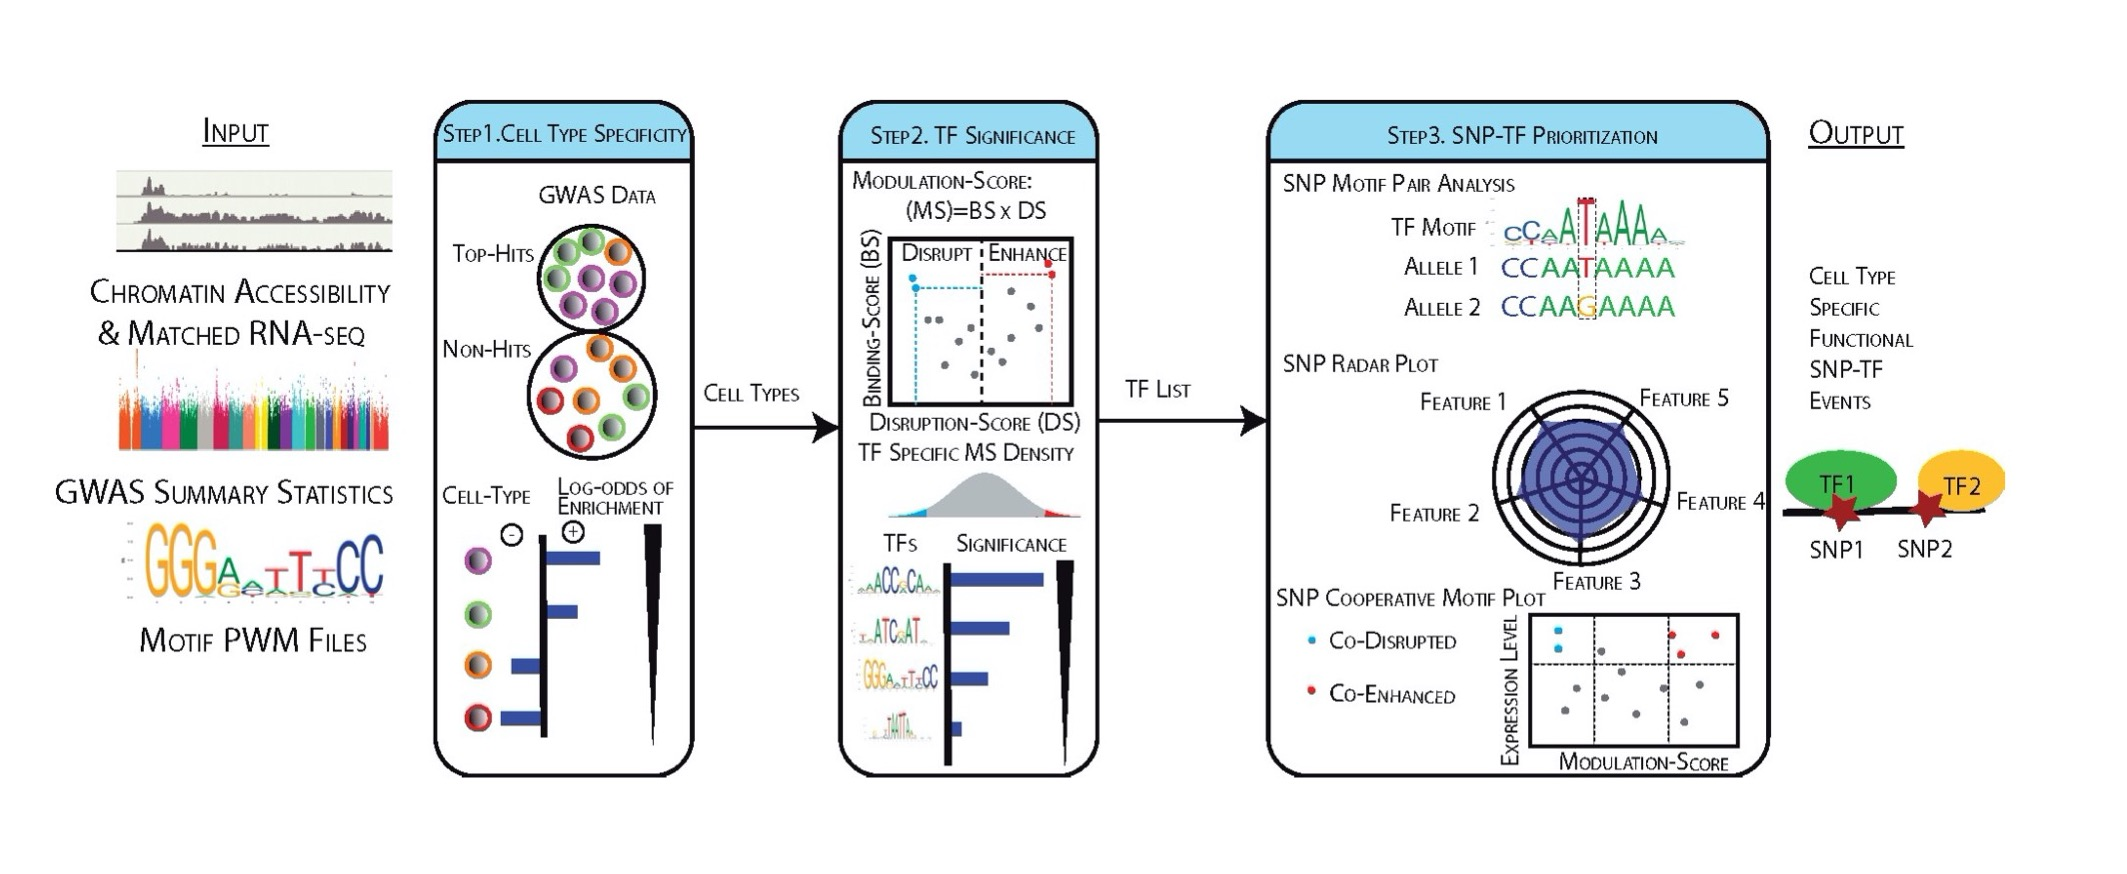
\includegraphics[width=\textwidth]{figures/motifraptor1.jpg}
    \caption[\motifraptor analysis pipeline]{\textbf{\motifraptor analysis pipeline.} \motifraptor executes a three-step process to enhance its functionality: (i) characterization of pertinent cell types, determined by the enrichment of trait-associated SNPs within chromatin accessible sites; (ii) identification of TFs with binding sites significantly influenced by genetic variants in these cell types; and (iii) pinpointing and visually representing individual TF-SNP regulatory events (taken from \cite{yao2021motif}).}
    \label{fig:motifraptor-pipeline}
\end{figure} 

% ---- Quantifying genetic variants impact on Transcription Factor Binding Sites
\subsection{Quantifying genetic variants impact on Transcription Factor Binding Sites}\label{subsection:motifraptor-quantifying-genetic-variants-impact}
To evaluate the impact of genetic variants on TFBS, \motifraptor implements an efficient and comprehensive genome-wide scoring procedure. \motifraptor scoring procedure scans all binding sites overlapping the input variants. Although the scanning procedure is similar to the algorithm implemented by other motif scanning algorithms, such as MOODS \citep{korhonen2009moods}, FIMO \citep{grant2011fimo} or \grafimo \citep{tognon2021grafimo}, \motifraptor proposes a threshold-free scanning. Threshold-free motif scanning enables to efficiently compute modulation scores and null models, used to test scores statistical significance. Given a genomic sequence $s$, where $|s|=m$, and a PWM, the score $M(i,S_{i})$ denotes the likelihood of observing the nucleotide $S_{i}\in\{A,C,G,T\}$ at position $i$, where $1 \leq i \leq m.$ We derive the binding score BS from $M(i,S_{i})$ as a log-likelihood score computed over the entire binding site and corrected to account for genome-wide nucleotide frequencies, or background frequencies, $B(s_{i})$:
\[
	\text{BS} = \log{\prod^{m}_{i=1}{\frac{M(i,s_{i})}{B(s_{i})}}} = \sum^{m}_{i=1}{(\log{M(i, s_{i}))} - \log{B(s_{i})})}
\] 
Based on this formulation, \motifraptor computes a disruption score DS, which reflects the potential impact of genetic variants on a given binding site. Given a target variant, \motifraptor assumes two haplotypes, denoted as $s_{ref}$ and $s_{alt}$ for the reference and alternative alleles, respectively. \motifraptor assigns a BS to each allele, resulting in binding scores for the reference and alternative alleles (i.e.  $\text{BS}(s_{ref})$ and $\text{BS}(s_{alt})$). To ensure computational scalability, \motifraptor restricts the calculations to a region spanning 61 bp, centered around the target variant. For each region, \motifraptor considers the best putative binding position $K$ for both $s_{ref}$ and $s_{alt}$:
\[
	K = \argmax_{1 \leq k \leq m}(\text{BS}(s_{ref, k:k+m-1}, M), \text{BS}(s_{alt, k:k+m-1}, M))
\]
Therefore, the disruption score DS at position $K$ is defined as:
\[
	\text{DS} = \Delta \text{BS}
\]
The magnitude and sign of DS are valuable indicators, conveying information about the direction and strength of the target variant's impact on TF binding. Specifically, positive DS suggest an increased binding affinity, while negative values imply a reduced binding potential. Since TFBS motifs exhibit varying length and specificity, \motifraptor scales both BS and DS to the ranges $[0,1]$ and $[-1,1]$, respectively:
\[
    \text{BS}_{\max}(M) = \max_{s_{i} \in \{A, C, G, T\}} \sum^{m}_{i=1}{\log{M(i,s_{i})}-\log{B(s_{i})}} 
\]
\[
    \text{DS}_{\max}(M) = \max_{s \neq w \in \{A, C, G, T\}}|\log{M(i, s_{i})} - \log{M(i, w_{i})}|
\]
Given the scaled scores, \motifraptor establishes a Binding-Disruption (BD) space. The BD-space offers a comprehensive framework to visualize and summarize TF-SNP modulation events globally and across different factors. Within the BD-space, events located near the distal corners from the origin (coordinates $(1,1)$ or $(1,−1)$) signify robust binding and substantial modulation induced by genetic variants. Furthermore, \motifraptor combines BS and DS into a composite score, called modulation score (MS):
\[
    \text{MS}(s, M) = \left(\frac{\text{BS}(s,M)}{\text{BS}_{\max}(M)}\right) \times \left(\frac{\text{DS}(s,M)}{\text{DS}_{\max}(M)}\right)
\]
MS encapsulates the rectangular area spanned by the scaled DS and BS. Larger absolute MS values, correspond to events close to the distal corners, and indicate meaningful modulation. Since no parametric distributions adequately fit the observed data, \motifraptor proposes to determine the statistical significance of SNP-TF modulation events, by estimating a null model based on the central limit theorem (CLT). However, this strategy involves a complete enumeration of all potential binding sites across the genome. \motifraptor overcomes this issue by leveraging efficient data structures, that efficiently compute genome-wide BS and DS for all input SNPs and TFs. Importantly, \motifraptor avoids to rely on pre-determined scores, $P$-value cutoffs, or computationally intensive shuffling procedures. Moreover, \motifraptor generates a ranked list of transcription factors built defining a TF score, that combines its cell type-specific expression and MS in chromatin accessible regions. Since TFs may share similar motifs but their expression and function is different across cellular contexts, the TF score, given a motif $M$ and a cell type $C$, is defined as:
\[
    \text{TF-score}(M,C) = \text{EP}(M,C) \times (1-\min{\text{FDR}(M,C)})
\] 
where the TF-score is constrained in $[0,1]$, $\text{EP}(M,C)$ is the expression percentile, and $\min{\text{FDR}(M,C)}$ is the corrected $P$-value for MS significance. $\min{\text{FDR}(M,C)}$  compares MSs' distribution in cell type-specific chromatin accessible regions.

% ---- Fast genome-wide motif scanning
\subsection{Fast genome-wide motif scanning}
The construction of a null model to statistically evaluate the BD-space and MS requires the exhaustive enumeration of all potential TFBS across the genome coupled with an assessment of their potential modulation by SNPs unrelated to any phenotype. While tools like FIMO or MOODS offer fast binding site occurrences enumeration, they are not optimized to efficiently compute the modulation of binding affinity induced by a set of SNPs \citep{zuo2015atsnp}. \grafimo partially overcomes this limitation, by considering genetic variation while searching motif occurrences (\textbf{Chapter 5}). However, some downstream analysis is required to recover the binding affinity modulation induced by genetic variants. MOODS, FIMO or \grafimo rely on a pre-defined threshold on statistical significance ($P$-value or $q$-value) to filter potential false positives or enhance computational efficiency. However, this strategy may exclude weak but genuine binding events \citep{boeva2016analysis,tognon2023survey}. In \motifraptor context, if employed, this strategy may bias the estimation of the complete empirical distribution of MSs. Moreover, establishing a uniform threshold for different TFBS motifs is neither practical nor reasonable \citep{tognon2023survey}. In fact, different TFBS display varying length and complexity. atSNP \citep{zuo2015atsnp} addresses the first challenge by proposing an efficient $P$-value estimation procedure. However, it lacks an effective threshold-free scanning technique. On the other hand, \motifraptor overcomes these limitation by avoiding redundant calculations. To avoid redundant calculations, \motifraptor leverages two text-indexing data structures: a suffix array (SA) \citep{puglisi2007taxonomy} and a longest common prefix (LCP) array \citep{landau2001linear}. SA and LCP enables bypassing of repeated portions of the genome, significantly reducing redundancy in calculations. \motifraptor algorithm performing fast genome-wide motif scanning encompasses different steps (\textbf{Algorithm \ref{alg:motifraptor-motif-scanning}}). \motifraptor starts by recovering all input SNPs and their flanking genomic sequences. Let us assume $N$ input variants and that the length of the flanking sequences surrounding each SNP is $2m-1$, where $m = |M|$. \motifraptor enrich each reference sequence with its linked variant returning two sequences: $s_{\text{ref}}$ and $s_{\text{alt}}$. Subsequently, $s_{\text{ref}}$ and $s_{\text{alt}}$ are concatenated constructing a single sequence, and the original sequences' genome positions are recorded. This results in a unique extended pseudo-genome ($P$) of length $2 \times (2m-1) \times N$. \motifraptor then computes the SA and LCP arrays on $P$ in linear time and space ($O(mN)$), using the divsufsort algorithm \citep{fischer2017dismantling}. By leveraging SA and LCP data structures, \motifraptor scan sequences in lexicographical order. Let us assume the algorithm is at iteration $j$ and it inductively computed an auxiliary array $\text{BS}[1:m]$, storing binding scores between $M$ and the first $m$ nucleotides in $P$ starting at position $\text{SA}[j-1]$. Then, $\text{BS}[m]=BS(P[\text{SA}[j-1]])$ against entire $M$. At iteration $j=0$, \motifraptor fills BS with 0s. At iteration $j=1$, \motifraptor inductively computes $\text{BS}[1:m]$ for the first $m$ nucleotides of suffix $\text{SA}[j]$. The existing values in $\text{BS}[1:m]$ referring to $\text{SA}[j-1]$ and the $\text{LCP}[j]$ value are exploited for efficient computation. If the common prefix's length between $\text{SA}[j-1]$ and $\text{SA}[j]$ is $p=\text{LCP}[j]$, the update of binding scores can start from position $p+1$, since the binding scores in $\text{BS}[1:p]$ remain unchanged, given that $\text{SA}[j-1]$ and $\text{SA}[j]$ share the initial $p$ characters for which binding scores have already been computed, $\text{BS}[1:p]$. Explicitly, for $p+1 \leq x \leq m$:
\[
    \text{BS}[x] = \text{BS}[p] + \sum^{x}_{i=p+1}{\log{M(i,s_{i})} - \log{B(s_{i})}}
\]
To map the binding score $\text{BS}[m]$ relative to an substring $s$, where $s \in P$ and $|s| = m$, aligned against the motif $M$, back to the SNP site, \motifraptor determines the SNP position and the binding position according to:
\[
    \text{SNP} = \left \lfloor \frac{\text{SA}[j]}{2m-1} \right \rfloor
\]
\[
    \text{binding\_site} = \text{SA}[j]\mod{(2m-1)}
\]
It is fundamental to note that not all prefixes $w$, where $|w|=m$, of $P$’s suffixes are substrings of the original genome. Recall that $P$ is constructed by concatenating sequences blocks centered around SNP positions. \motifraptor further improves the running time by skipping cross-block sequences scanning. By exploiting these data structures and score design, \motifraptor efficiently compute genome-wide binding and disruption scores for each TF, enabling complete null models estimation factor.

% - algorithm: MotifRaptor motif scanning algorithm
\begin{algorithm}[!]
    \caption{\motifraptor motif scanning algorithm}
    \label{alg:motifraptor-motif-scanning}
    \KwData{SNPs, $G$, $M$}
    \KwResult{$\text{BS}$}
    $P \gets \text{computePseudoGenome}(\text{SNPs}, G, M)$ \Comment*[r]{see algorithm \ref{alg:motifraptor-pseudogenome}}
    $\text{SA} \gets \text{computeSuffixArray}(P)$ \Comment*[r]{use divsufsort algorithm}
    $\text{LCP} \gets \text{computeLCP}(P, \text{SA})$\;
    $\text{BS} \gets \text{initializeArray}(0, |P|)$\;
    \For{$i \in \text{|BS|}$}{
        $\text{BS}[i] \gets \text{scoreSequence}(P[i:i+m], M, \text{SA}[i-1], \text{LCP}[i])$\;
    }
    \Return{$\text{BS}$}
\end{algorithm}

% - algorithm: Algorithm computing Pseudo-genome P
\begin{algorithm}[!]
    \caption{Algorithm computing Pseudo-genome $P$}
    \label{alg:motifraptor-pseudogenome}
    \KwData{SNPs, $G$, $M$}
    \KwResult{$P$}
    $m \gets |M|$\;
    $P \gets \emptyset$\;
    \For{$\text{snp} \in \text{SNPs}$}{
        $s_{\text{ref}} \gets G[\text{snp}_{\text{pos}} - m:\text{snp}_{\text{pos}} + m]$\;
        $s_{\text{alt}} \gets \text{enrichSequence}(s_{\text{ref}},\text{snp})$\;
        $s \gets \text{concatenate}(s_{\text{ref}}, s_{\text{alt}})$\;
        $P \gets \text{concatenate}(P,s)$\;
    }
    \Return{$P$}
\end{algorithm}

% ---- Evaluating TF-SNP modulations significance
\subsection{Evaluating TF-SNP modulations significance}
To assess the statistical significance of TF-SNP modulation scores (MSs), \motifraptor employs a method leveraging the central limit theorem (CLT). This involves estimating a complete null model through the enumeration of all potential binding sites across the genome. To ensure scalability, \motifraptor leverages suffix and LCP arrays, that enable exhaustive enumeration while maintaining method's scalability. For a given set of target variants $V$, \motifraptor evaluates whether they significantly modulate TF binding events by testing if MS distribution $D_{\text{MS}}(V)$ significantly differs from the MS distribution obtained from a set of background (genome-wide) SNPs $W$ ($D_{\text{MS}}(W)$). To assess the distinction between the distributions, \motifraptor employs a non-parametric test with a null hypothesis: 
\[
    E(D_{\text{MS}}(V))=E(D_{\text{MS}}(W))
\]
According to CLT, the distribution of the sample mean of $W$, converges to a normal distribution, with its mean equal to $E(D_{\text{MS}}(W))$, and variance equal to $\frac{\Var({D_{\text{MS}}(W)})}{N_{\text{sample}}}$, regardless of the underlying MS distribution. Consequently, \motifraptor assesses the significance of enhanced scores $E(D_{\text{MS}}(V))$, disrupted scores $E(D_{\text{MS}}(W))$, or both. This robust procedure, combined with efficient data structures, enables the identification of significant genome-wide shifts in TF-SNP binding modulations without relying on predetermined scores or cutoffs on $P$-values.

% ----- MotifRaptor helps prioritizing variants affecting Transcription Factor Binding Sites involved in LDL-C uptake
\section{\motifraptor helps prioritizing variants affecting Transcription Factor Binding Sites involved in LDL-C uptake}
We demonstrate the capabilities of \motifraptor by utilizing the tool to prioritize potential TFs modulated by a set of lipoprotein cholesterol (LDL-C)-associated GWAS variants and low-density lipoprotein receptor (LDLR) coding variants on LDL-C uptake in HepG2 hepatocellular carcinoma cells. Genetic differences in LDL-C levels significantly impact the risk of coronary artery disease. This is supported by quantitative serum LDL-C measurements, which are consistently recorded across various biobanks, making them one of the most reliable human phenotypic datasets available. Through a trans-ancestry GWAS meta-analysis conducted by the Global Lipids Genetics Consortium (GLGC), over 900 genome-wide significant loci associated with blood lipid levels have been identified, with more than 400 loci specifically linked to LDL-C \citep{graham2021power}. Notably, these LDL-C GWAS loci exhibit a significant overlap with gene expression patterns in the liver, suggesting the liver's pivotal role in modulating the effects of LDL-C variants \citep{wang2022epic,finucane2018heritability}. Despite this correlation, the specific causal variants and mechanisms underlying many of these loci's influence on LDL-C levels remain elusive. LDL-C levels are profoundly influenced by rare coding variants, with the most severe cases linked to Familial Hypercholesterolemia (FH), a disease characterized by markedly elevated LDL-C levels and premature cardiovascular disease \citep{bouhairie2015familial}. FH arises from inherited monogenic variants in several genes, primarily affecting LDLR, a cell surface receptor pivotal for LDL uptake, thereby regulating its circulation levels \citep{brown1984ldl}. Despite the efficacy of lipid-lowering therapies, individuals with FH still face a significantly heightened risk of coronary events compared to the general population \citep{mundal2018impact}. Given that elevated LDL-C levels elevate cardiovascular disease risk across the lifespan, early identification of at-risk individuals holds paramount clinical significance \citep{bouhairie2015familial}. However, many LDLR variants currently lack clear clinical interpretation. For instance, among the 1,427 LDLR missense variants cataloged in the ClinVar database \citep{landrum2020clinvar}, half are designated as variants of unknown significance (VUS) or exhibit conflicting interpretations of pathogenicity, thereby complicating FH diagnosis. Similarly, within the UK Biobank cohort \citep{bycroft2018uk}, 69\% of the 758 unique LDLR missense variants carried by sequenced individuals lack reporting or have uncertain annotations in ClinVar. 
%
% - figure: BEAN computational-experimental base editing screening pipeline
\begin{figure}[!]
	\centering
	\includegraphics[width=\textwidth]{figures/crisprbean-pipeline.png}
	\caption[BEAN computational-experimental base editing screening pipeline]{\textbf{BEAN computational-experimental base editing screening pipeline. (A)} The plot illustrates the process and analysis workflow for activity-normalized base editing screening, followed by analysis using BEAN. Initially, a library of gRNAs, each coupled with a reporter sequence containing its genomic target, is inserted into a lentiviral base editor expression vector. Lentiviral transduction is conducted in HepG2 cells, succeeded by flow cytometric sorting of four distinct populations based on fluorescent LDL-cholesterol (BODIPY-LDL) uptake levels. Paired-end NGS is then employed to decode gRNA counts and reporter editing outcomes within each flow cytometric bin. Subsequently, BEAN is utilized to model the editing frequency of the reporter and allelic outcomes, along with gRNA enrichments across flow cytometric bins. This enables BEAN to estimate variant phenotypic effect sizes. \textbf{(B)} The sequence logo illustrates the adjacent nucleotide specificity of ABE8e-SpRY editing, derived from 7,320 gRNAs. In the logo, the height of each base symbolizes the relative frequency of observing that particular base given an edit at position 0. \textbf{(C)} Average editing efficiency of ABE8e-SpRY by protospacer position and PAM sequence. \textbf{(D)} The scatterplots illustrate the comparison of nucleotide-level editing efficiency between the reporter and endogenous target sites across three experimental replicates for a total of 49 gRNAs spanning four loci. The top panel displays the accessibility of the four loci as measured by ATAC-seq signal in HepG2 cells, with scatterplot markers colored according to the accessibility of each nucleotide. Pearson correlation coefficients ($r$) are provided to indicate the strength of correlation between the editing efficiency of reporter and endogenous target sites. \textbf{(E)} The schematic depicts the design of the LDL-C variant library gRNA, targeting selected GWAS candidate variants. The Manhattan plot illustrates variant P-values obtained from a recent GWAS study \citep{klimentidis2020phenotypic}. The gRNAs are strategically designed to tile the variant at five positions, maximizing editing efficiency at protospacer positions 4–8. \textbf{(F)} gRNA coverage of the LDLR tiling library across LDLR coding sequence along with 5’ and 3’ UTRs and several regulatory regions.}
	\label{fig:bean-pipeline}
\end{figure}
%
A more comprehensive understanding of the impacts of LDLR variants would facilitate the earlier diagnosis and treatment of numerous individuals at risk for FH and associated cardiovascular complications. To assess the effects of both common GWAS-associated and rare coding variants in the LDLR gene, we developed a novel approach, called BEAN \citep{ryu2023joint}, leveraging base editing techniques (\textbf{Section \ref{subsection:base-editing}}) followed by the cellular uptake of fluorescent LDL-C in HepG2 cells (\textbf{Figure \ref{fig:bean-pipeline}}). BEAN offers a scalable flow cytometric assay to measure a critical determinant of serum LDL-C levels \citep{hamilton2023systematic}, as the liver plays a predominant role in clearing LDL-C from circulation \citep{spady1992hepatic}. Our experimental-computational pipeline enables us to scrutinize LDL uptake-altering GWAS-associated variants and elucidate their downstream effects on chromatin accessibility, transcription factor binding, and gene expression, ultimately impacting LDL uptake. Intriguingly, we identify causal variants that influence LDL-C uptake by affecting the genes OPRL1, VTN, and ZNF329, which were not previously linked to LDL-C levels.

% ---- Evaluating candidate variants impact on Transcription Factor Binding potential 
\subsection{Evaluating candidate variants impact on Transcription Factor Binding potential}
% - table: LDL-C uptake associated variants prioritized through BEAN and tested for Transcription Factor binding modulation
\begin{table}[!]
    \centering
    \resizebox{\columnwidth}{!}{%
    \begin{tabular}{|l|l|l|l|l|l|l|l|}
        \hline
        \textbf{Variant} &
          \textbf{Chrom} &
          \textbf{Position (hg38)} &
          \textbf{\begin{tabular}[c]{@{}l@{}}Major\\ Allele\end{tabular}} &
          \textbf{\begin{tabular}[c]{@{}l@{}}Minor\\ Allele\end{tabular}} &
          \textbf{\begin{tabular}[c]{@{}l@{}}HepG2 Editable \\ REF Allele\end{tabular}} &
          \textbf{\begin{tabular}[c]{@{}l@{}}HepG2 Edited\\ Allele\end{tabular}} &
          \textbf{MAF} \\ \hline
        rs4149309   & chr9  & 104,827,299 & \texttt{A}      & \texttt{T} & \texttt{A} & \texttt{G} & 0,11951 \\ \hline
        rs12042481  & chr1  & 45,499,094  & \texttt{T}      & \texttt{C} & \texttt{T} & \texttt{C} & 0,169   \\ \hline
        rs186701924 & chr19 & 56,948,710  & \texttt{A}      & \texttt{C} & \texttt{A} & \texttt{G} & 0,00125 \\ \hline
        rs4457349   & chr8  & 125,482,075 & \texttt{A}      & \texttt{G} & \texttt{A} & \texttt{G} & 0,0259  \\ \hline
        rs429358    & chr19 & 44,908,684  & \texttt{T}      & \texttt{C} & \texttt{T} & \texttt{C} & 0,156   \\ \hline
        rs11149612  & chr16 & 83,947,360  & \texttt{C}      & \texttt{T} & \texttt{T} & \texttt{C} & 0,461   \\ \hline
        rs4719853   & chr7  & 26,029,463  & \texttt{T}      & \texttt{A} & \texttt{T} & \texttt{C} & 0,237   \\ \hline
        rs76895963  & chr12 & 4,275,678   & \texttt{T}      & \texttt{G} & \texttt{T} & \texttt{C} & 0,02104 \\ \hline
        rs35081008  & chr19 & 58,150,868  & \texttt{C}      & \texttt{T} & \texttt{T} & \texttt{C} & 0,147   \\ \hline
        rs58198139  & chr5  & 156,972,028 & \texttt{C}      & \texttt{T} & \texttt{T} & \texttt{C} & 0,364   \\ \hline
        rs1250259   & chr2  & 215,435,759 & \texttt{T}      & \texttt{A} & \texttt{A} & \texttt{G} & 0,265   \\ \hline
        rs704       & chr17 & 28,367,840  & \texttt{G}      & \texttt{A} & \texttt{A} & \texttt{G} & 0,474   \\ \hline
        rs77542162  & chr17 & 69,085,137  & \texttt{A}      & \texttt{G} & \texttt{A} & \texttt{G} & 0,0229  \\ \hline
        rs1434282   & chr1  & 199,041,592 & \texttt{C}      & \texttt{T} & \texttt{T} & \texttt{C} & 0,274   \\ \hline
        rs8126001   & chr20 & 64,080,106  & \texttt{C}      & \texttt{T} & \texttt{T} & \texttt{C} & 0,48964 \\ \hline
        rs10107182  & chr8  & 58,480,178  & \texttt{C}      & \texttt{T} & \texttt{T} & \texttt{C} & 0,336   \\ \hline
        rs62084210  & chr17 & 67,832,594  & \texttt{A}      & \texttt{G} & \texttt{A} & \texttt{G} & 0,29613 \\ \hline
        rs771555783 & chr17 & 80,025,096  & \texttt{CACCAT} & \texttt{C} &   &   & 0,224   \\ \hline
        rs115421711 & chr5  & 52,787,392  & \texttt{A}      & \texttt{G} & \texttt{A} & \texttt{G} & 0,0413  \\ \hline
        rs3767844   & chr1  & 214,007,378 & \texttt{A}      & \texttt{G} & \texttt{A} & \texttt{G} & 0,28746 \\ \hline
        rs2618566   & chr20 & 17,864,040  & \texttt{G}      & \texttt{T} & \texttt{T} & \texttt{C} & 0,339   \\ \hline
        rs4390169   & chr1  & 155,133,578 & \texttt{A}      & \texttt{G} & \texttt{A} & \texttt{G} & 0,481   \\ \hline
        rs402348    & chr18 & 63,367,187  & \texttt{T}      & \texttt{G} & \texttt{T} & \texttt{C} & 0,211   \\ \hline
        rs116734477 & chr5  & 52,799,190  & \texttt{C}      & \texttt{T} & \texttt{T} & \texttt{C} & 0,0412  \\ \hline
    \end{tabular}%
    }
    \caption[LDL-C uptake associated variants prioritized through BEAN and tested for Transcription Factor binding modulation]{\textbf{LDL-C uptake associated variants prioritized through BEAN and tested for Transcription Factor binding modulation.} The table provides details of genetic variants linked to LDL-C uptake, which were prioritized using BEAN \citep{ryu2023joint}. These variants underwent testing for modulation of Transcription Factor binding using \motifraptor \citep{yao2021motif}. It includes information such as the genomic location (hg38 genome assembly), major and minor alleles on both the reference genome and HepG2 cells, as well as the minor allele frequency (MAF) associated with each variant. MAF values are sourced from the UK Biobank cohort \citep{bycroft2018uk}.}
    \label{tab:bean-variants}
\end{table}
%
To investigate the potential effects of LDL-C uptake-associated variants, prioritized using BEAN (\textbf{Table \ref{tab:bean-variants}}), on transcription factor binding sites and their regulatory impact on genes involved in LDL-C uptake, we adapted the pipeline of \motifraptor for our analysis. Each variant's genomic context was investigated by retrieving sequences spanning 61 bp centered around the SNP location. To recover the genomic context we used the GRCh38 genome assembly as reference. For each variant, we generated both a reference and an alternative sequence by substituting the major allele with the minor allele at the SNP position. Subsequently, we employed all human TF PWMs from the CIS-BP database \citep{weirauch2014determination} to scan each pair of reference and alternative sequences, generating binding scores for each major and minor allele. The comparison of these scores for each TF across the reference and alternative alleles within every sequence pair was crucial for assessing a variant's impact on TF binding. Higher binding scores for the alternative sequence indicated an increase in TF binding potential, while lower scores suggested a decrease. To quantify these changes, we computed disruption scores (DS) (\textbf{Section \ref{subsection:motifraptor-quantifying-genetic-variants-impact}}). Recall, that DS captures the directional change induced by each variant, where a negative value signifies reduced TF binding potential, and a positive value indicates an increase. For each variant, we ranked TFs exhibiting heightened binding potential and susceptibility to disruption by the variant. In the case of rs8126001, our methodology highlighted two zinc finger TFs, ZNF333 and ZNF770, showcasing enhanced binding site sequences attributed to the presence of the heterozygous minor allele in HepG2 cells (\textbf{Figure \ref{fig:crisprbean-motifraptor-ds}}). HepG2 ChIP-seq data provides supportive evidence for the binding of these TFs at the locus, even though the variant lies at the periphery of the peaks (\textbf{Figure \ref{fig:crisprbean-chip-variant}}). While drawing definitive conclusions necessitates additional experimental validation, our findings are consistent with prior research \citep{farh2015genetic}, which implies that a minority of causal variants directly modify canonical TF binding sequences. Instead, the majority tend to influence non-canonical sequences, emphasizing the intricacies involved in understanding the impact of genetic variants on transcription factor interactions.

% - figure: MotifRaptor analysis reveals insights into potential disruption of transcription factor binding by candidate variants.
\begin{figure}[!]
	\centering
	\includegraphics[width=\textwidth]{figures/crisprbean-motifraptor-ds.png}
	\caption[\motifraptor analysis reveals insights into potential disruption of transcription factor binding by candidate variants]{\textbf{\motifraptor analysis reveals insights into potential disruption of transcription factor binding by candidate variants. (A)} The disruption is graphically represented against the binding scores of motifs, specifically examining the transition from the minor to major allele of rs8126001. \textbf{(B-C)} The identified motifs of ZNF333 and ZNF770 are showcased, aligned with the loci of rs8126001, featuring both minor and major alleles.}
	\label{fig:crisprbean-motifraptor-ds}
\end{figure}

% - figure: An overview of ChIP-seq signal Log2 Fold Change (LFC), signal $P$-values, peaks, and motif occurrences is provided for ZNF333 and ZNF770 in proximity to rs8126001
\begin{figure}[!]
	\centering
	\includegraphics[width=\textwidth]{figures/crisprbean-chip-rs8126001.png}
	\caption[An overview of ChIP-seq signal Log2 Fold Change (LFC), signal $P$-values, peaks, and motif occurrences is provided for ZNF333 and ZNF770 in proximity to rs8126001]{\textbf{An overview of ChIP-seq signal Log2 Fold Change (LFC), signal $P$-values, peaks, and motif occurrences is provided for ZNF333 and ZNF770 in proximity to rs8126001}. PhastCons100way conservation scores and gene annotations are co-displayed. ENCODE accession numbers are encapsulated in parentheses. The ENCODE signal LFC and $P$-values are derived through the ENCODE processing pipeline, utilizing MACS2 \citep{zhang2008model} for the generation of signal $P$-values.}
	\label{fig:crisprbean-chip-variant}
\end{figure} 


% -- Improving MotifRaptor by employing SVM-based motif models
\subsection{Improving MotifRaptor by employing SVM-based motif models}
In the case study presented in the original paper, \motifraptor's predictions were supported by literature, suggesting that it leverages promising ideas. However, \motifraptor’s main limitation is the employed computational models to represent TF binding motifs. Despite position weight matrices \citep{stormo2000dna} (PWMs) are simple, intuitive, and widely employed TF motif models, PWMs carry several drawbacks that often result in under- or over-estimation of non-coding variant impact on TFs binding landscape \citep{tognon2023survey}. TF SVM-based motif models \citep{tognon2023survey, boeva2016analysis} have been demonstrated to overperform PWMs in several tasks, such as prediction of binding events and variants impact on TF binding sequences. However, while several publicly available resources provide complete and extensive collections of motif PWMs, to our knowledge there is no complete collection of SVM-based TF motifs. Therefore, we propose an extensive and curated collection of SVM-based motifs as well as a novel approach to annotate the functional impact of non-coding variants on TF binding landscape using SVM-based models, which interpolates different omics data, such as transcriptome, DNase-seq \citep{john2011chromatin}, ATAC-seq \citep{buenrostro2013transposition}, etc. 
% - Building a library of transcription factor SVM-based models
\subsubsection{Building a library of transcription factor SVM-based models}
SVM-based models have demonstrated superior performance compared to traditional PWMs \citep{tognon2023survey}. However, a significant drawback persists as no motif database currently offers these advanced SVM-based models. Moreover, the interpretability of these models remains a challenging issue, and there is a scarcity of motif analysis tools that harness the power of SVMs-based motif models. To address these limitations,  we propose the creation of a comprehensive library comprising SVM-based motif models. To compute the SVM-based motif models we use ChIP-seq data from ENCODE \citep{encode2012integrated}.  To enhance model reproducibility, we modified FactorBook's model computation pipeline \citep{pratt2022factorbook} (\textbf{Fig.\ref{fig:motifraptor3}}).
\begin{figure}
	\centering
	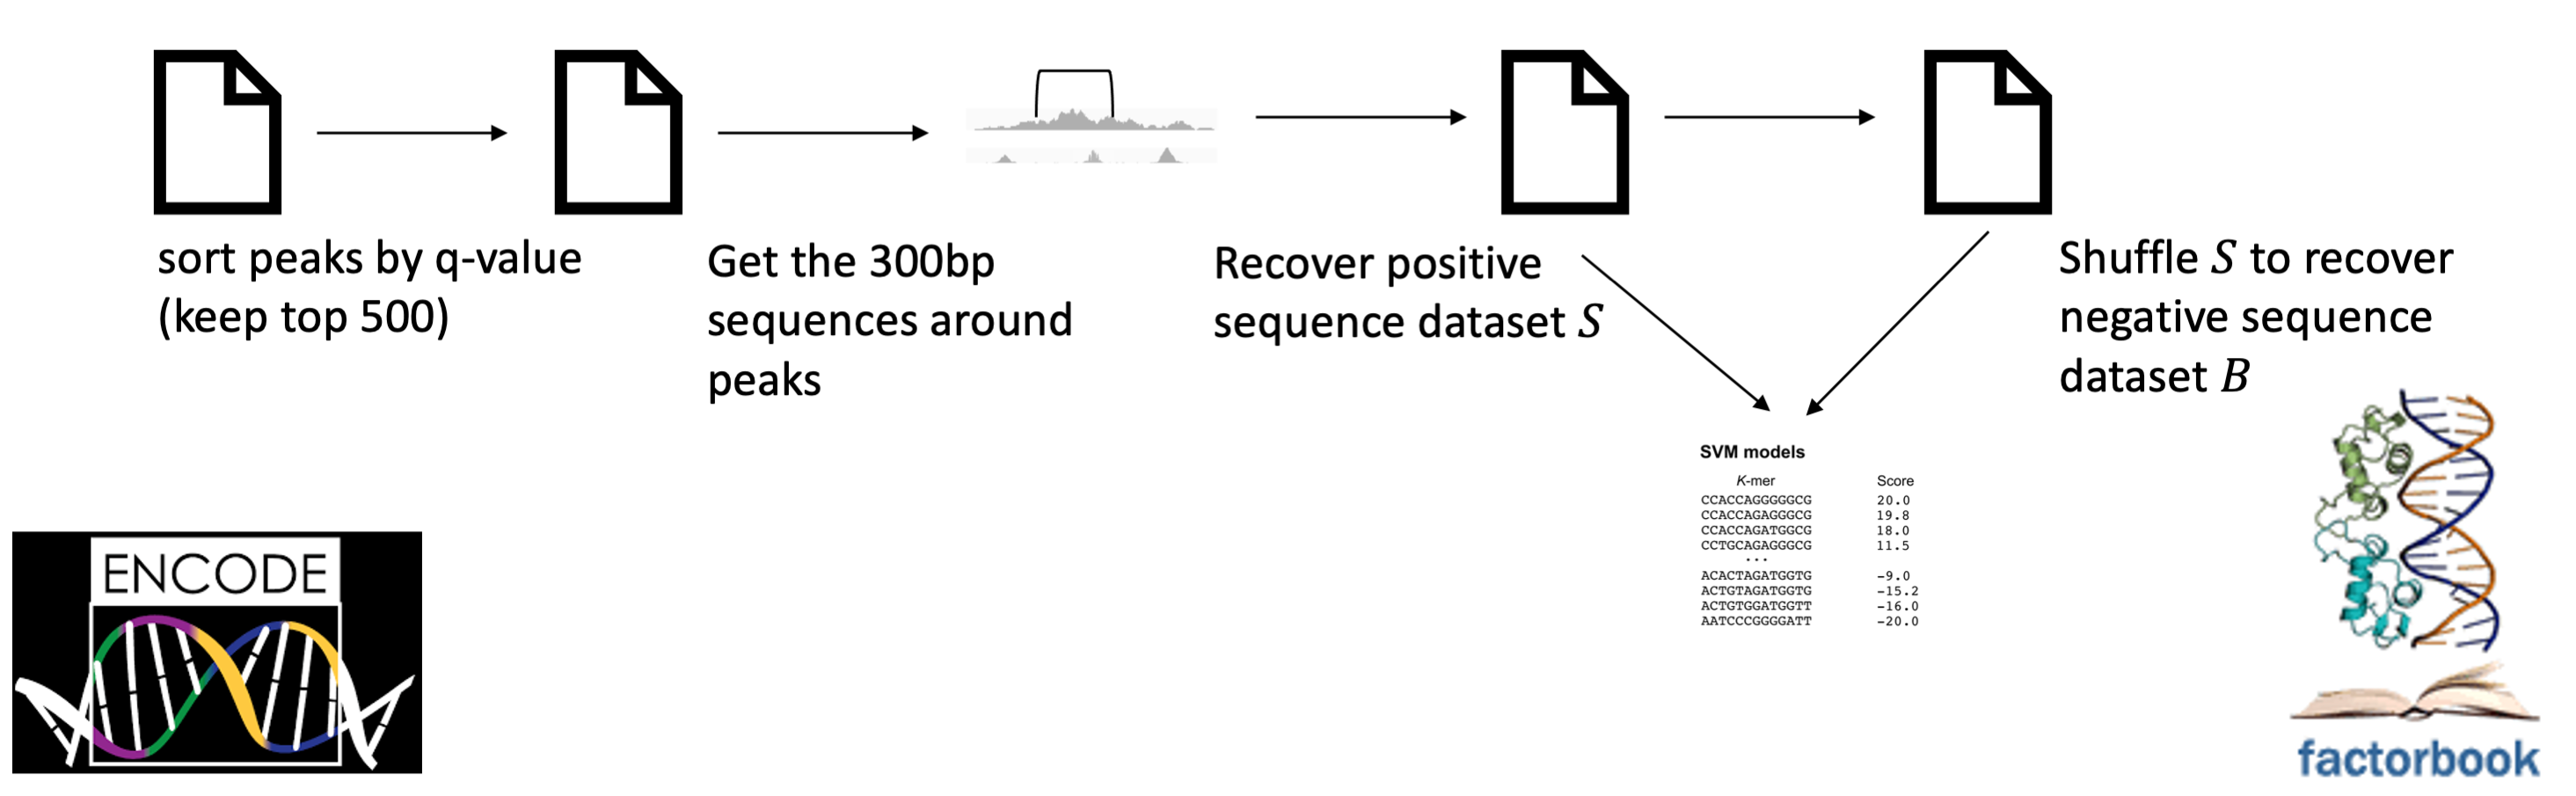
\includegraphics[width=\textwidth]{figures/motifraptor3.png}
	\caption[SVM-based motif models computation workflow]{\textbf{SVM-based motif models computation workflow.} For the sake of reproducibility, we follow the model computation pipeline employed by FactorBook database, to derive PWM models from ENCODE data.}
	\label{fig:motifraptor3}
\end{figure} 
To compute the models we selected ChIP-seq peaks datasets from ENCODE retrieved on different tissues and cell types.  For each ChIP-seq dataset, we selected the top 500 peak sequences sorted by $q$-value. Then, we shrinked the surviving peaks to 300 bp centered around the peak signal center. After recovering the resulting genomic sequences, we constructed a background dataset by shuffling the original sequences. The two dataset are, then, used as input to compute the SVM models using LS-GKM \citep{lee2016ls}.
% - Comparing SVM-based and PWM motif models predictive power
\subsubsection{Comparing SVM-based and PWM motif models predictive power}
\begin{figure}
	\centering
	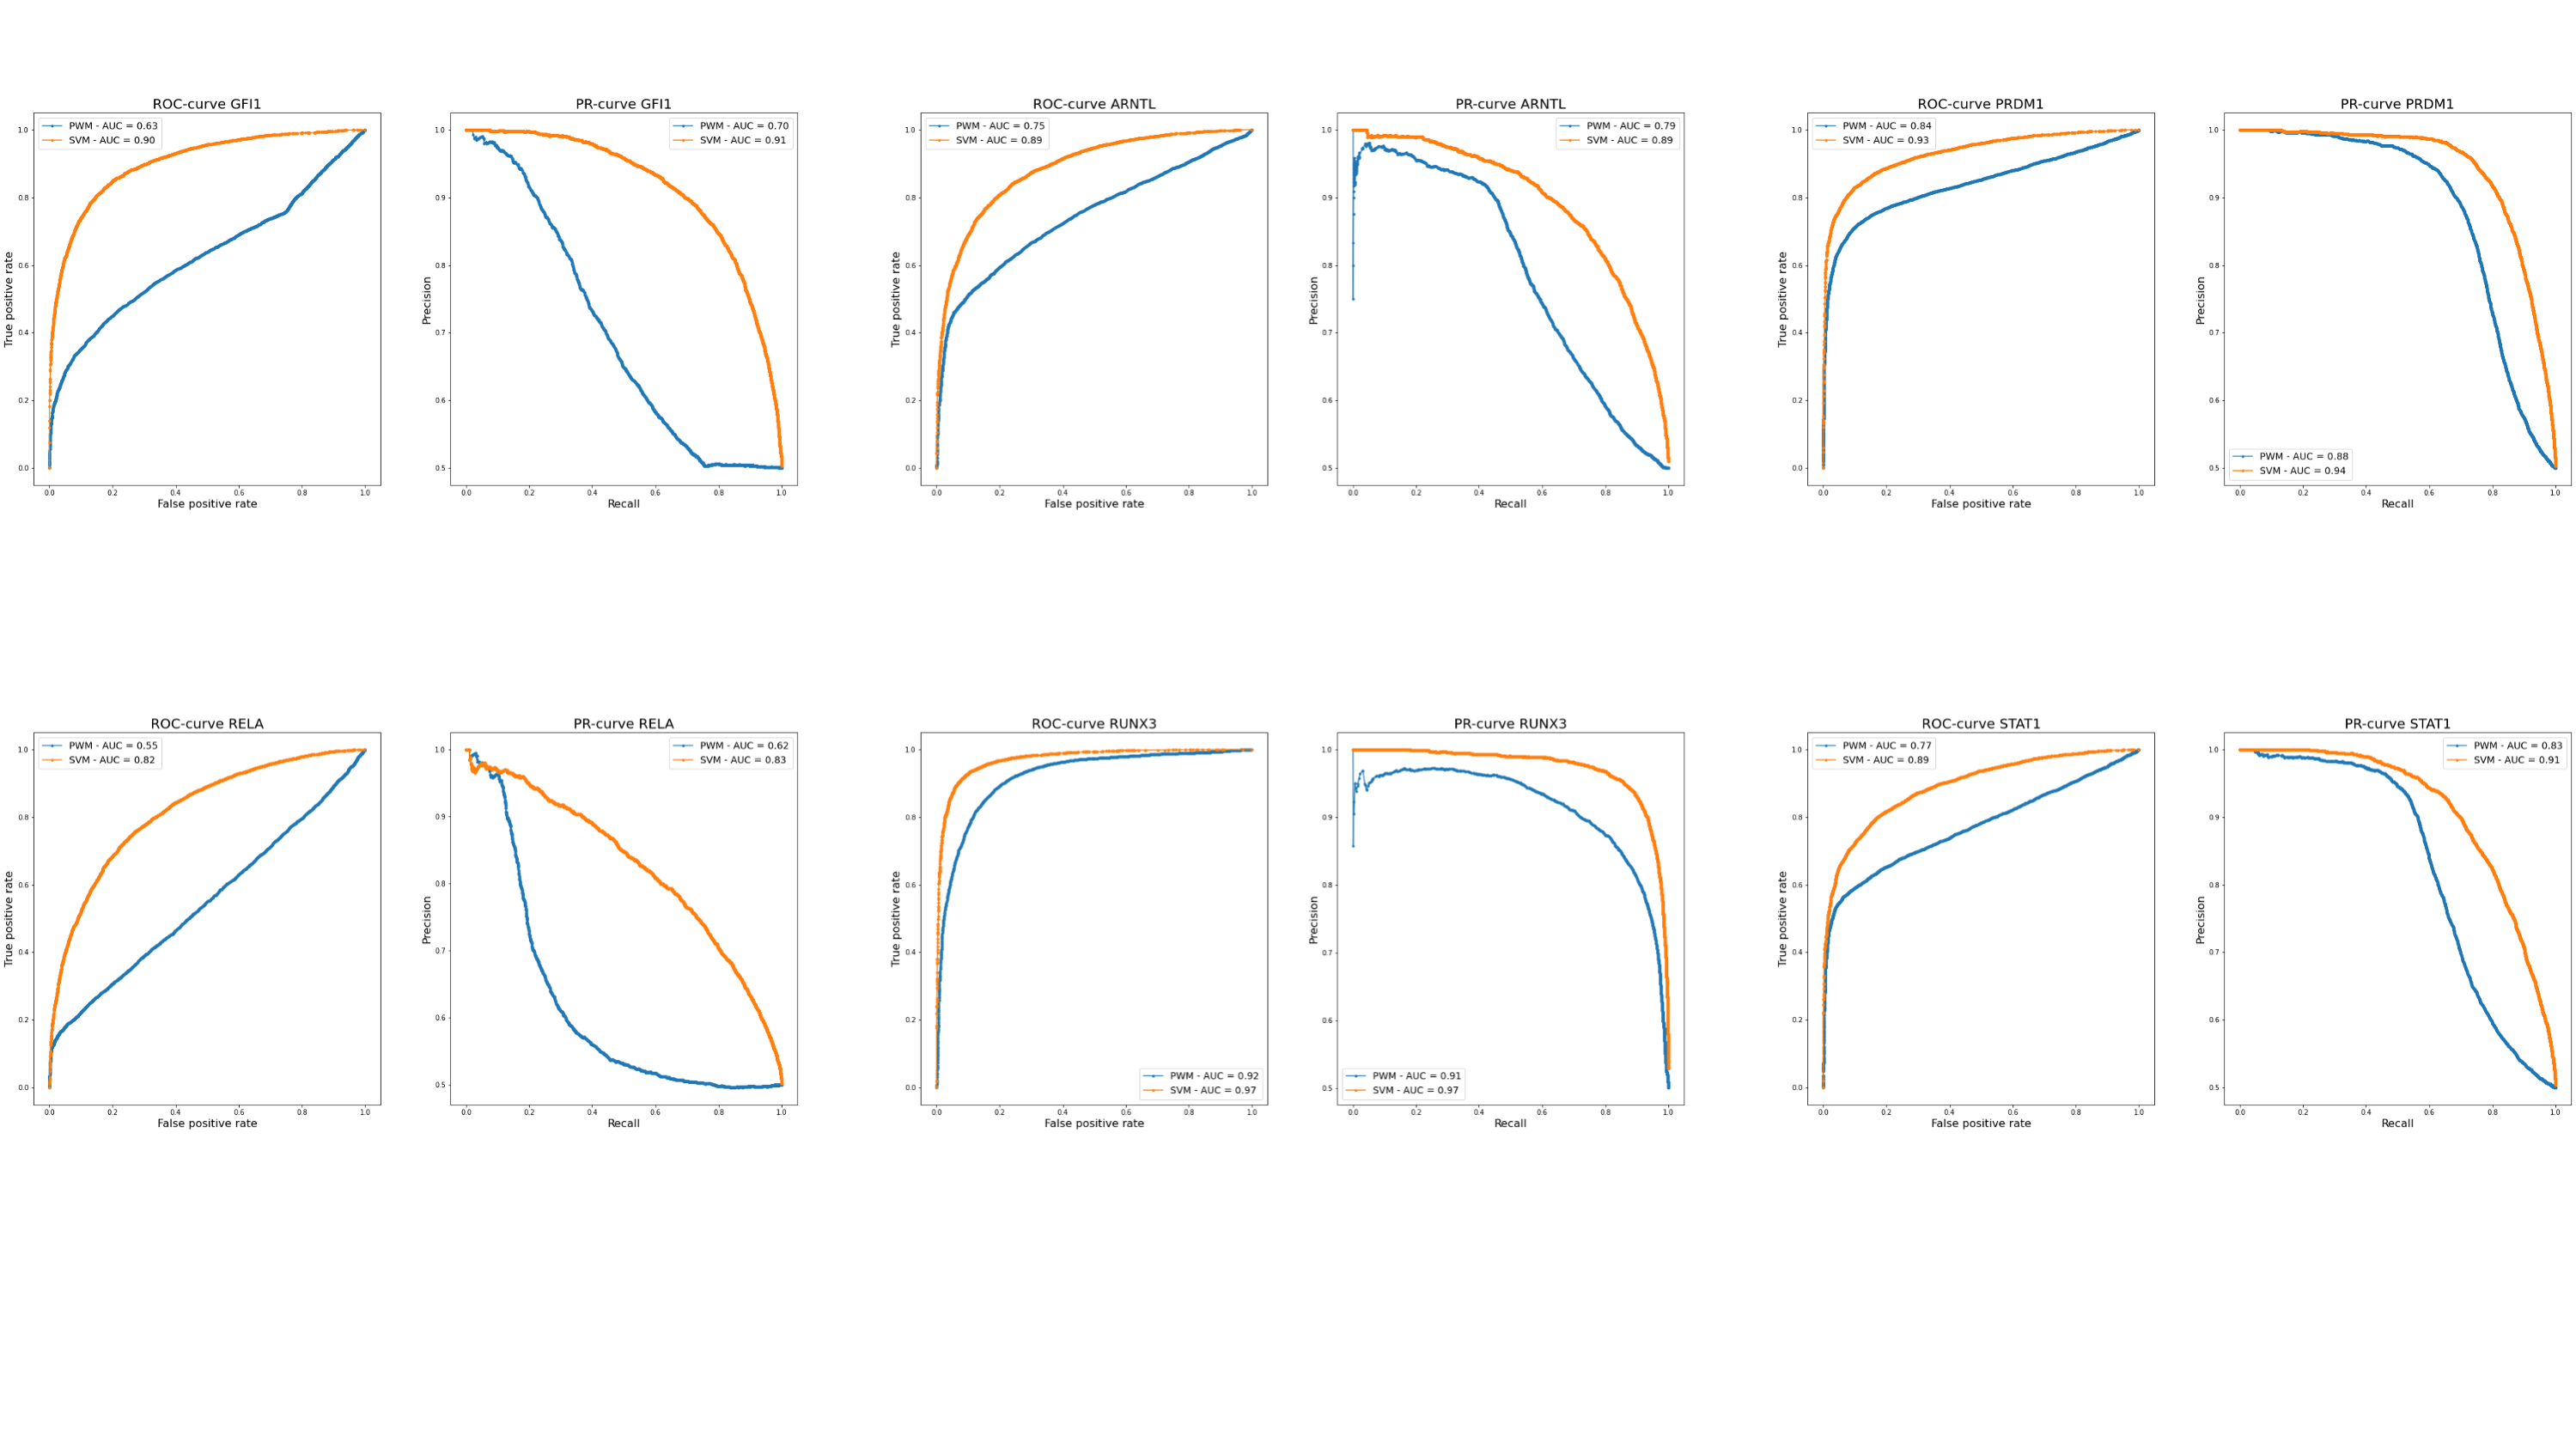
\includegraphics[width=\textwidth]{figures/motifraptor2.png}
	\caption[Comparing SVM-based and PWM motif models predictive power]{\textbf{Comparing SVM-based and PWM motif models predictive power.} We compared the predictive power of SVM-based and PWM motif models for six transcription factors: ARNTL, GFI1, PRDM1, RELA, RUNX3 and STAT1. Both models were trained on ENCODE ChIP-seq data (cell line GM12878). To train SVM-based models we followed the described pipeline, while to train PWM models we replaced LS-GKM with MEME. The predictive perfomance of the two models have been compared computing ROC- and PR-curves.}
	\label{fig:motifraptor2}
\end{figure} 
We demonstrate the improvements brought by SVM-based motif models over PWMs, by comparing the predictive power of the two models in terms of ROC- and PR-curves. For this analysis we selected the six TFs that have been previously identified in the original \motifraptor publication to be affected by mutations linked to rheumatoid arthritis: ARNTL, GFI1, PRDM1, RELA, RUNX3, and STAT1. For the assessment we employed the original and the modified FactorBook pipeline, where the latter replaces MEME with LS-GKM to compute the SVM models. MEME \citep{bailey1994fitting} is a widely used software to compute PWM motif models from sequence data. To train and test the models we selected one ChIP-seq dataset for each TF (GM12878 cell line) from the ENCODE data portal. After training, we compared models' performance via a $4$-fold cross-validation (75\% training and 25\% testing) on the top 500 peaks, selected following FactorBook's pipeline. By running our comparison, we observed that generally SVM-base motif models better predict binding events than PWMs, in both terms of ROC and PR-curves (\textbf{Fig.\ref{fig:motifraptor2}}).
% -- Future directions
\subsection{Future directions}
In the next future we plan to complete our SVM-based motif models catalog extending the presented analysis to all the remaining TFs whose ChIP-seq data are available in ENCODE. Additionally, ENCODE datasets could be integrated employing datatasets from different databases, such as Cistrome \citep{zheng2019cistrome} or GTRD \citep{kolmykov2021gtrd}. Moreover, we plan to release to the community the complete SVM motif models catalog. We also plan to train models on SELEX data rather than ChIP-seq and compare the resulting models. Importantly, since SELEX is a method less susceptible to noise than ChIP-seq the resulting models could potentially provide an even larger boost of models' predictive performance. We plan to modify \motifraptor scanning algorithm for both PWM and SVM motif models to consider haplotypes, and indels. In fact,  currently \motifraptor consider only SNP and treats them as independent events, however it is known that complex SNP-SNP, SNP-indel, indel-indel combination can happen \citep{tognon2021grafimo}, often with signifcant effects on TF binding potential.


% ------ CRISPR Genome Editing
\mychapter{7}{CRISPR genome editing}
The discovery of the Clustered Regularly Interspaced Short Palindromic Repeats (CRISPR)-Cas system has revolutionized genetic engineering, offering a precise, versatile and programmable framework to modify the genomes of living organisms \citep{cong2013multiplex}. Originally identified in bacterial immune system \citep{garneau2010crispr}, CRISPR-Cas system has become a transformative gene-editing tool with profound implications for molecular biology and the potential for innovative therapeutic interventions \citep{jinek2012programmable,hsu2014development,kantor2020crispr}. CRISPR-Cas systems encompass an ensemble of diverse components each employing distinct mechanisms of action. Despite different Cas proteins (\textbf{Table \ref{tab:cas-pam}}) may be employed depending on the editing goal \citep{makarova2020evolutionary}, all systems rely on CRISPR RNA (crRNA) for precise target specificity. Notably, some variants introduce an additional requirement for trans-activating RNA (tracrRNA), forming a crucial scaffold structure \citep{kantor2020crispr}. The aforementioned CRISPR RNAs are joined into a single small guide RNA (sgRNA) \citep{ran2013genome}. Using sgRNAs rather than crRNAs and tracrRNAs significantly simplifies the editing process design. Protospacer adjacent motif (PAM) sequences are other key components of most CRISPR-Cas systems. PAM sequences are short motifs adjacent to the target sequence, restricting Cas proteins action to locations presenting the target sequence followed by the appropriate PAM. The simplicity of the 5'-\texttt{NGG}-3' PAM sequence requirement has led to the predominant use of Streptococcus pyogenes' Cas9 (SpCas9) protein in different applications (\textbf{Figure \ref{fig:crispr-cas9} (A)}). However, spCas9's PAM sequence significantly restricts its editing landscape. Consequently, recent studies focused on proposing novel engineered Cas proteins enhancing Cas9 editing scope \citep{anders2016structural,miller2020continuous}. Notably, the SpG and SpRY Cas9 variants significantly expanded the editing landscape \citep{walton2020unconstrained}, targeting less stringent PAMs. SpG is designed to target an expanded set of \texttt{NGN} PAMs. SpRY is a nearly PAM-less variant (PAM \texttt{NRN}) enabling to edit regions previously considered "un-targetable". By delivering the Cas9 nuclease complex coupled with a synthetic sgRNA (Cas9:sgRNA) CRISPR provides a simple and programmable means to modify genomic sequences at specific locations (\textbf{Figure \ref{fig:crispr-cas9} (B)}). To perform its editing action, the Cas9:sgRNA complex engages in a randomized exploration of the cellular DNA, initially seeking the appropriate PAM. Upon locating the PAM sequence, Cas9 unwinds the DNA to facilitate the hybridization of the Cas9-associated sgRNA with the exposed DNA strand, known as the protospacer. When the DNA sequence aligns with the sgRNA target sequence, the catalytic domains of the endonuclease execute the cleave the DNA double strand, resulting in a double-strand break \citep{jinek2012programmable}. Subsequently, the host cell undertakes the repair of this break through either non-homologous end joining (NHEJ) or homology-directed repair (HDR) mechanisms (\textbf{Figure \ref{fig:crispr-cas9} (C-D)}). Genome editing mediated by other Cas proteins works similarly. While NHEJ leads to insertions or deletions at the repair site, HDR can be employed to insert a defined DNA template, to precisely repair the edited DNA segment. However, HDR pathway exhibits limited efficiency and high rates of unintended indels mutations, potentially compromising the mutation repairing \citep{mao2008comparison,song2017optimizing}. CRISPR-Cas-mediated single-base-pair editing (DNA base-editors) systems have been developed to address these limitations \citep{nishida2016targeted,kantor2020crispr}. There are two classes of base-editors (BEs): cytosine base-editors (CBEs) and adenine base-editors (ABEs). CBEs and ABEs can introduce all four nucleotide transitions. The introduction of prime-editors (PEs) broadened the spectrum of donor-free precise DNA editing. In fact, PEs not only cover all nucleotide transitions and transversions but also extend their capability to handle small insertion and deletion mutations \citep{anzalone2019search}. CRISPR-Cas systems empower precise yet potentially random sequence editing, the experiment success relies on metculous design of guide sgRNAs to direct the Cas complex to the intended target sequences (\emph{on-targets}). Achieving this precision is crucial to avoid unintended and potentially risky alterations in non-targeted sequences (\emph{off-targets}) \citep{pattanayak2013high,cho2014analysis}. Additionally, genetic variants may introduce novel unexpected target sites and PAMs, potentially influencing experiment outcome \citep{scott2017implications}. As a result, while designing sgRNA designs it becomes imperative to consider genetic diversity, especially in clinical applications, to prevent potential undesired and hazardous consequences within the host genome. In aiding the design of suitable sgRNAs, various computational approaches have emerged. Guide-design tools primarily focus on computationally predicting potential guide RNAs that can target a specified input sequence, such as a gene or regulatory element, given a PAM. In parallel, off-target nomination tools offer insight into the potential sequences edited using a specific sgRNA and PAM sequence within a host genome. These tools furnish a list of both the intended target sequence and potentially unintended edited sequences. Furthermore, additional tools have been developed to assist researchers in evaluating and quantifying the success of their CRISPR genome editing experiments by analyzing the observed editing events in their data. Altogether, CRISPR genome editing has the potential to revolutionize the precision medicine paradigm. Its ability to make targeted modifications to the genome presents a powerful framework for addressing diseases linked to individual-specific molecular reasons \citep{sgro2020epigenome,ho2020enabling}. Beyond disease correction, CRISPR-based interventions hold promise in advancing our understanding of intricate genetic and epigenetic mechanisms underlying various health conditions \citep{syding2020crispr}. Moreover, the adaptability of CRISPR technologies allows for the exploration of therapeutic avenues in the context of genetic disorders, neurodegenerative diseases \citep{kolli2018application}, and even certain types of cancer \citep{wang2022current}, paving the way for innovative and personalized treatment strategies. Additionally, the continuous refinement of CRISPR tools and the exploration of new delivery methods contribute to the ongoing evolution of this revolutionary technology, expanding its potential applications in diverse biomedical and therapeutic realms. The subsequent sections delve into the fundamental components of the Cas9 complex (with similar principles applicable to systems employing different Cas proteins), explore Base Editors (BEs) and Prime Editors (PEs) along with their distinctions from other CRISPR-Cas systems, address the off-target problem, and present an overview of computational methods available for the analysis of CRISPR genome editing experiment data.

% - table: Cas nucleases and their PAM sequences
\begin{table}[]
    \centering
    \begin{tabular}{|l|l|}
        \hline
        \textbf{Nuclease} & \textbf{PAM}          \\ \hline
        spCas9            & \texttt{NGG}          \\
        SpCas9-VQR        & \texttt{NGAG}         \\
        spCas9-VRER       & \texttt{NGCG}         \\
        spCas9-NG         & \texttt{NGN}          \\ 
        spCas9-xCas9      & \texttt{NG}/\texttt{GAA}/\texttt{GAT}   \\ 
        spCas9-Sc++       & \texttt{NNG}          \\ 
        {\ul spCas9-SpG}  & \texttt{NGN}          \\ 
        {\ul spCas9-SpRY} & \texttt{NRN}          \\ 
        SaCas9            & \texttt{NNGRRT}       \\ 
        SaCas9-KKH        & \texttt{NNNRRT}       \\ \hline
        AsCas12a          & \texttt{TTTV}         \\ 
        AsCas12a-RR       & \texttt{TYCV}         \\ 
        AsCas12a-RVR      & \texttt{TATV}         \\ 
        Cas12j            & \texttt{TTN}          \\ 
        Cas12e            & \texttt{TTCN}         \\ \hline
        Un1Cas12f1        & \texttt{TTTN}         \\ 
        CnCas12f1         & \texttt{CCN}          \\ \hline
    \end{tabular}%
    \caption[Cas nucleases and their PAM sequences]{\textbf{Cas nucleases and their PAM sequences.} List of different Cas nucleases and their Protospacer Adjacent Motif (PAM) sequences. Underlined Cas proteins denote ``near PAM-less'' nucleases}
    \label{tab:cas-pam}
\end{table}

% - figure: CRISPR-Cas9 genome editing
\begin{figure}[!]
	\centering
	\includegraphics[width=\textwidth]{figures/crispr_cas9_genome_editing.png}
	\caption[CRISPR-Cas9 genome editing]{\textbf{CRISPR-Cas9 genome editing. (A)} X-Ray resolved structure of SpCas9 nuclease (obtained from the PDB database, accession number 6VPC \citep{lapinaite2020dna}). \textbf{(B)} sgRNA:Cas9 complex. The sgRNA guides Cas9 to its target sequence. Once the sgRNA is paired with the target sequence, Cas9 opens the double-stranded DNA (dsDNA) near the Protospacer Adjacent Motif (PAM) sequence. After unwinding the DNA, Cas9 cleaves the dsDNA 3-4 bp upstream with respect to the PAM sequence, inducing a DNA breakage. The DNA breaks are repaired through either: \textbf{(C)} Non-homologous End Joining (NHEJ), which introduces insertions or deletions (indels) in the edited sequences, or \textbf{(D)} Homologous Directed Repair (HDR), which inserts a template DNA within the edited segment.}
	\label{fig:crispr-cas9}
\end{figure} 

% ----- Essential elements in CRISPR-Cas9 Genome Editing
\section{Essential elements in CRISPR-Cas9 Genome Editing}
SpCas9  popularity in several CRISPR genome editing applications is mainly attributed to the simplicity of its 5'-\texttt{NGG}-3' PAM sequence and its widespred availability (\textbf{Figure \ref{fig:crispr-cas9}}). The precision of CRISPR-Cas9 editing systems hinges on two crucial factors \citep{ran2013genome}: (i) the target sequence, a 20 bp string within each CRISPR locus of the sgRNA array, which typically has multiple unique targets, and (ii) the PAM sequence, which Cas9 identifies to initiate editing. Once identified its target sequences, Cas9 nuclease opens both DNA strands to introduce novel and precise modifications. Cas9 operates primarily through two mechanisms: (i) knock-in and (ii) knock-out mutations. In knock-in, HDR employs DNA sequences that resemble the target to mend the Cas9-induced breaks in the genome, using exogenous DNA as a template for repair. Conversely, in knock-out, the mutations in the DNA introduced by Cas9 result in the repair of breaks via NHEJ. Repair through NHEJ often leads to random indels in the target sequence, which can disrupt, enhance, or alter the function of the targeted site.

% ---- The Cas9 nuclease
\subsection{The Cas9 nuclease}
Cas9 is a protein that holds a crucial role in the immune defense mechanisms of certain bacteria against DNA viruses and plasmids. Widely utilized in genetic engineering applications, its primary function revolves around cleaving DNA, enabling modifications to a cell's DNA sequence. To survive in diverse and challenging environments populated with bacteriophages, certain bacteria have evolved mechanisms to resist and repel predatory viruses. The CRISPR system serves as a fundamental element in these defense strategies. Functionally, CRISPR-Cas systems act as self-programmable restriction enzymes. CRISPR loci consist of short, palindromic repeats occurring at regular intervals, comprising alternating CRISPR repeats and variable CRISPR spacers ranging from 24 to 48 bp in length. Typically, CRISPR loci are accompanied by adjacent CRISPR-associated (cas) genes, which encode DNA restricting enzymes, such as SpCas9 in Streptococcus pyogenes (\textbf{Figure \ref{fig:crispr-cas9} (A)}). The discovery that spacer regions within CRISPR loci exhibit homology to foreign DNA elements, including plasmids and viruses, marked the first biological evidence suggesting that CRISPRs might function as an immune system, providing bacteria with a versatile and adaptive defense mechanism against viral intruders. This discovery laid the foundation for applying the CRISPR-Cas system to edit genome sequences \citep{mali2013cas9}. Cas9, a dual RNA-guided DNA endonuclease enzyme associated with the CRISPR adaptive immune system in Streptococcus pyogenes, plays a pivotal role in this system (\textbf{Figure \ref{fig:crispr-cas9} (B)}). In Streptococcus pyogenes, CRISPR memorizes foreign DNA, while Cas9 functions as an executor, interrogating and cleaving intruding DNA \citep{garneau2010crispr,jinek2012programmable,heler2015cas9}. Cas9's interrogation involves unwinding foreign DNA and scrutinizing it for sites that align with the 20 bp spacer region of the guide RNA (gRNA). Upon identifying complementarity, Cas9 executes the cleavage of the invading DNA. Beyond its role in bacterial immunity, Cas9 has emerged as a robust genome engineering tool, inducing site-directed double-strand breaks in DNA. These breaks can lead to the inactivation of genomic functional elements or the introduction of foreign segments through non-homologous end joining (NHEJ) or homology-directed repair (HDR), respectively (\textbf{Figure \ref{fig:crispr-cas9} (C-D)}). Cas9's popularity has surged due to its capability to cleave nearly any sequence complementary to the guide RNA \citep{jinek2012programmable}. Importantly, its target specificity relies on guide RNA:DNA complementarity rather than modifications to the protein itself. This unique feature makes Cas9 directly applicable to target DNA sequences \citep{mali2013cas9}. The original bacterial Cas9 requires a guide RNA composed of two distinct RNAs: the CRISPR RNA (crRNA) and the trans-activating crRNA (tracrRNA) \citep{deltcheva2011crispr}. To simplify Cas9 DNA targeting, chimeric single guide RNAs (sgRNAs) have been engineered. These advancements underscore the versatility and potential of Cas9 as a powerful tool in genetic engineering and genome editing \citep{ran2013genome}.

% ---- sgRNA: guiding Cas9 to target sequences
\subsection{sgRNA: guiding Cas9 to target sequences}\label{subsection:sgrna}
Guide RNAs (sgRNAs) are RNA segments that serves as a guiding tool for enzymes, such as Cas nucleases, targeting RNA or DNA sequences \citep{ran2013genome}. By forming complexes with Cas enzymes, sgRNAs guide the sgRNA:Cas complex to the intended target sequences to edit (\textbf{Figure \ref{fig:crispr-cas9} (B)}). While guide RNAs have natural occurrences and play crucial roles in various biological functions, sgRNAs are synthetically designed in genome editing applications to achieve precise and targeted modifications. sgRNAs achieve targeting through straightforward Watson-Crick base pairing with complementary sequences. Through complementary base-pairing sgRNAs direct Cas enzymes to the specific target region. sgRNAs are synthetically designed by joining two RNAs: (i) the trans-activating RNA (tracrRNA), and (ii) the  CRISPR RNA (crRNA) \citep{deltcheva2011crispr}. The tracrRNA facilitates Cas9 endonuclease activity, while the crRNA binds to the target-specific DNA segments. tracrRNA possesses a stem-loop structure, serving as the base-pairing partner for the endonuclease enzyme. crRNA contains a spacer-flanked region resulting from repeat sequences, comprising 18-20 bp. crRNA recognizes the specific complementary target region, initiating cleavage by Cas9 upon binding with the crRNA and tracrRNA effector complex. Modifications in the crRNA sequences enable changes in the target regions, rendering it a user-defined programmable tool. sgRNAs design is crucial for the precision of CRISPR-mediated genome editing experiments. For instance, in CRISPR-Cas9 regions targeting is dictated by the 20 bp sequence at the 5' end of sgRNA. However, to ensure cleavage the target sequence must be followed by the Protospacer Adjacent Motif (PAM). PAMs are short DNA segments located immediately after the target region. PAMs are crucial for Cas nucleases to cleave targets and are generally located 3-4 bp downstream from the cleavage site. 

% ---- Protospacer Adjacent Motifs
\subsection{Protospacer Adjacent Motifs}\label{subsection:pam}
Protospacer Adjacent Motifs (PAMs) (\textbf{Figure \ref{fig:crispr-cas9} (B)}) constitute a 2–6 bp DNA sequence positioned immediately following the sequence targeted by Cas nucleases \citep{shah2013protospacer}. Notably, PAMs are absent in the bacterial host genome, despite their integration into the invading virus or plasmid. The effective binding and cleavage of the target DNA sequence by Cas proteins hinge on the presence of the PAM sequence following it \citep{jinek2012programmable,shah2013protospacer}. In fact, Cas9 refrains from cleaving the target sequence unless there is an immediately adjacent PAM sequence. Serving as an indispensable targeting component, PAM plays a pivotal role in discerning bacterial self from non-self DNA, thereby shielding the CRISPR locus from being targeted and disrupted by the CRISPR-associated nuclease. In CRISPR-Cas9 genome editing applications, sgRNAs recognize target sequences with a \texttt{NGG} PAM sequence at the 3'-end, guiding the nuclease to a specific sequence for cleavage \citep{cong2013multiplex}. After sgRNA-target pairing, Cas9 starts breaking the DNA double strand 3-4 bp upstream the PAM location. Crucially, most Cas proteins start editing exclusively at sites where they recognize a PAM. Numerous endeavors have been undertaken to engineer SpCas9 and other Cas nucleases capable of recognizing various PAMs, with the goal of enhancing the versatility of CRISPR genome editing at specified locations within the genome \citep{kleinstiver2015engineered} (\textbf{Table \ref{tab:cas-pam}}).

% ----- Precision Genome Editing: Maintaining DNA Double Strand Structure with Base-Editing and Prime-Editing
\section{Precision Genome Editing: Maintaining DNA Double Strand Structure with Base-Editing and Prime-Editing}
While Homologous Directed Repair (HDR) can insert DNA templates within edited sites to accurately restore genome sequences, this pathway is hindered by restricted efficiency and elevated rates of undesirable indel mutations. These mutations often offset the potential advantages gained from the mutation repair process \citep{kantor2020crispr}. Additionally, HDR-mediated editing is constrained to cell types that are actively dividing, as it heavily relies on homologous recombination processes \citep{bollen2018create}. The introduction of base-editing (BE) and prime-editing (PE) systems addressed these issues, introducing frameworks to precisely edit the genome sequence without breaking double strand DNA \citep{komor2017crispr,anzalone2019search}. Importantly, BEs and PEs have potential to rectify disease-causing mutations within the human genome. Targeting the four transition mutations enables the correction of over 25\% of human pathogenic SNPs. By inserting or deleting short DNA segments beside targeting the four nucleotide transitions, PEs may address up to 89\% of known genetic variants linked to human diseases \citep{komor2017crispr,anzalone2019search,kantor2020crispr}. Therefore, BEs and PEs hold great promises in expanding the therapeutical significance of genome editing technologies. Notably, BEs and PEs may become fundamental tools in precision medicine settings and bring closer the realization of the paradigm \citep{porto2020base}. The next sections describe the main concepts behind BE and PE.

% ---- Base-editing
\subsection{Base-editing}\label{subsection:base-editing}
BE systems present similar components to CRISPR-Cas. However, beside encompassing a Cas enzyme, BEs include a single-stranded DNA modifying enzyme to precisely modify nucleotides. BEs are divided in two distinct classes based on the single-stranded DNA modifying enzyme: cytosine base-editors (CBEs) and adenine base-editors (ABEs). Collectively, CBEs and ABEs can perform all four nucleotide transitions ($\text{\texttt{C}} \rightarrow \text{\texttt{T}}$, $\text{\texttt{T}} \rightarrow \text{\texttt{C}}$, $\text{\texttt{A}} \rightarrow \text{\texttt{G}}$, $\text{\texttt{G}} \rightarrow \text{\texttt{A}}$). Furthermore, the introduction of dual base-editor systems designed for combinatorial editing within human cells, expanded BEs' scope incorporating transversions \citep{kurt2021crispr,grunewald2020dual,sakata2020base,zhang2020dual}. Such advances may facilitate targeting more intricate compound edits significantly expanding DNA BE landscape.

% --- Cytosine base-editors
\subsubsection{Cytosine base-editors}
Cytosine base-editors (CBEs) deaminate cytosine to uracil ($\text{\texttt{C}} \rightarrow \text{\texttt{U}}$), which is recognized as a thymine during cell replication. This process results in $\text{\texttt{C}} \rightarrow \text{\texttt{G}}$ and $\text{\texttt{T}} \rightarrow \text{\texttt{A}}$ transitions fixed in the DNA sequence after cell replication \citep{komor2016programmable,komor2017crispr}. The introduction of the engineered nCas9 protein dramatically improved CBE efficiency \citep{komor2016programmable}. This Cas9 variant induces a nick in the strand containing the \texttt{G} in the \texttt{U}-\texttt{G} intermediate. The nick on the non-edited DNA strand favors cellular repair towards a \texttt{U}-\texttt{A} outcome. The latter is subsequently transformed into \texttt{T}-\texttt{A} during DNA replication. Employing nCas9 resulted in a six-fold increase in editing efficiency. Despite nCas9 exhibited 1.1\% indel rate, it remains significantly lower compared to the rate induced by editing systems using HDR and breaking double strand DNA \citep{komor2016programmable}. Further improvements have been introduced to reduce indel rate \citep{kim2017increasing,kantor2020crispr}. In parallel, researchers focused on broadening the range of targetable bases, by developing BEs that incorporate different CRISPR nucleases. In fact, CBEs using SpCas9 face limitations due to their dependence on its \texttt{G}/\texttt{C}-rich PAM. To address the cahallenge a range of engineered Cas9 variants with modified PAM sequences and enhanced cleavage specificity has been developed. These variants hold the potential to further expand the targeting scope \citep{kim2020high,chatterjee2020engineered,miller2020continuous,zetsche2015cpf1}.

% --- Adenine base-editors
\subsubsection{Adenine base-editors}
Since their editing capabilities are constrained to install \texttt{C}-\texttt{G} to \texttt{T}-\texttt{A} mutation, CBEs present a limited spectrum of correction of disease-linked variants. Moreover, methylated cytosines are prone to spontaneous deamination \citep{alsoe2017uracil}, potentially introducing pathogenic variants. Adenine base-editors (ABEs) address these limitations by converting \texttt{A}-\texttt{T} to \texttt{G}-\texttt{C}. Importantly, this enable to potentially reverse $\sim$50\% of pathogenic SNPs. This development significantly broadened the scope of BEs applications to treatment of diseases with genetic and molecular bases. ABEs employ an ABE-dCas9 complex binding to a target DNA sequence guided by gRNA. The complex's deaminase domain catalyzes the transition of adenine to inosine, that is interpreted as guanine during DNA replication \citep{gaudelli2017programmable}. This facilitates the replacement of the original \texttt{A}-\texttt{T} with \texttt{G}-\texttt{C} at the targeted site. Generally, ABEs editing efficiency is high introducing almost no indels. While they worked well when paired with SpCas9, ABEs exhibited limited compatibility with Cas9 variants. ABE8e \citep{gaudelli2017programmable, richter2020phage} solved this issue, providing a base-editor with enhanced efficiency and compatibility with Cas9 variants other than SpCas9. This significantly expanded the editing landscape of ABEs, enabling the editing of a wide range of genomic regions.

% ---- Prime-editing
\subsection{Prime-editing}
Originally, CBEs and ABEs limited their editing capability to four transition mutations. Prime-editing (PE) \citep{anzalone2019search} addressed the issue proposing a BE method operating without inducing double-strand breaks in the DNA, and employing an engineered reverse transcriptase (RT). The RT is fused to Cas9 nickase (nCas9) and a prime-editing guide RNA (pegRNA) \citep{anzalone2019search}. pegRNAs have two major functions purpose: (i) directing nCas9 to the target site, and (ii) harboring an additional sequence specifying the desired sequence edits \citep{anzalone2019search}. Briefly, the 5′ end of the pegRNA binds to the primer binding site (PBS) region on the DNA. This bind induces the exposure of the non-complementary strand. Subsequently, Cas9 nicks the unbound DNA strand containing the PAM, creating a primer for the RT to start its retrotranscription. While elongating the nicked strand, RT uses the interior of the pegRNA as a template, editing the target region. This operation produces two redundant PAM DNA flaps: the edited 3′ and unedited 5' flaps. To include the edit within the DNA, PE exploits cellular endonucleases actions. In fact, The cell endonucleases are abundant during lagging-strand DNA synthesis, and preferentially degrade the 5′ flaps \citep{kantor2020crispr}. The resulting heteroduplex containing the unedited and the edited strands is resolved and integrated into the host genome through cellular replication and repair processes.

% ----- Editing unwanted regions: addressing the Off-Targets issue and understanding the influence of Genetic Diversity
\section{Editing unwanted regions: addressing the Off-Targets issue and understanding the influence of Genetic Diversity}\label{section:offtarget-problem}
CRISPR genome editing offers signifcant opportunities for developing innovative therapeutics by precisely modifying genetic or epigenetic elements, such as regulatory elements, within specific genomic regions. The design of gRNAs to precisely target the intended sequences (on-targets) is of paramount importance. gRNAs precision is essential to prevent unintended and potentially deleterious edits in non-targeted sequences, called off-targets \citep{pattanayak2013high,cho2014analysis}. Off-target edits often occur at sites exhibiting sequence homology to the intended on-target. However, the precise rules governing off-target editing remain unclear \citep{tycko2016methods}. The presence of mismatches in sequences may result in either a decrease in cleavage activity or may have no discernible effect, contingent upon the specific nature of the base alteration and its relative position \citep{doench2014rational,doench2016optimized}. Furthermore, while off-target editing generally decrease with the number of mismatches \citep{cho2014analysis}, several studies demonstrated that off-targets mutations occur in sites displaying up to 6 mismatches with respect to the on-target \citep{tsai2015guide}. Off-target prediction is a fundamental practice guiding the development and design of CRISPR experiment. Beyond the mere count of mismatches or bulges, various sequence characteristics, such as the position of the mismatch or bulge relative to the PAM, or specific base alterations, contribute to the likelihood of off-target effects. Notably, genetic diversity significantly influences the potential creation of new off-target sites \citep{scott2017implications}. Indeed, genetic variants can enhance the affinity of certain sequences previously unbound by the sgRNA. Furthermore, they may generate novel PAM sequences due to their simple structure. PAMs occurring in novel positions may induce Cas proteins to break double stranded DNA in previously uncut positions, with potential hazardous effects on the cell environment. Several methods are currently available to assess on- and off-target genome editing at individual loci \citep{clement2020technologies}. These approaches encompass both sequencing and non-sequencing-based methods. While non-sequencing-based methods, generally, provide cost-effective solutions to detect sequence edits, sequecing-based technologies precisely quantify editing frequencies and define the mutation alleles induced by genome editing \citep{clement2020technologies}. Among these methods, GUIDE-seq \citep{tsai2015guide} and Circle-seq \citep{tsai2017circle} have been succesfully employed to experimentally identify off-target edits \emph{in cellula} and \emph{in vivo}, respectively.  

% ----- The computational aspects of CRISPR Genome Editing experiments
\section{The computational aspects of CRISPR Genome Editing experiments}
Designing effective gRNAs is crucial for precisely targeting specific sequences within the genome while minimizing off-target effects. Several computational tools are to design guides (guide-designer). Guide-designer provide a list of potential guides targeting a region. However, these tools must account for potential off-target sites during gRNA design to mitigate unintended genetic alterations. Off-target nomination tools predict and analyze off-target effects of input gRNAs. They provide a comprehensive landscape of the potential experimental outcomes. CRISPR edits can be quantified using several tailored computational methods, that measure editing events from sequencing data. Although, quantification methods detect and quantify editing events in common CRISPR genome editing settings, they fall short when measuring the phenotypic outcomes in more compelx experiments, like CRISPR screens. CRISPR screens evaluate the impact of genetic variants on phenotypic traits, providing insights into the functionality of specific genomic elements and their implications for disease and therapeutics. 

% ---- Designing guide RNAs
\subsection{Designing guide RNAs}
Designing guide RNAs (gRNAs) to precisely target specific sequences within the genome is a critical aspect of planning CRISPR genome editing experiments. These gRNAs not only need to efficiently target the intended target sequence but also must minimize the risk of binding to unintended sites, thereby reducing the likelihood of off-target effects. To assist researchers in this endeavor, a variety of computational tools have emerged to facilitate the design of gRNAs with optimal characteristics \citep{li2023computational}. These tools, available both online and offline, leverage sophisticated algorithms to predict gRNA efficacy and specificity. Among the available tools, web-based platforms like CRISPOR \citep{haeussler2016evaluation}, CRISPR-SURF \citep{hsu2018crispr}, and CHOPCHOP \citep{montague2014chopchop} offer user-friendly interfaces for designing gRNAs. Additionally, specialized tools such as Prime-design \citep{hsu2021primedesign} cater to specific applications, such as designing pegRNAs used in PE experiments. A crucial aspect of these gRNA design tools is their ability to assess the off-target potential associated with the predicted guides. Once gRNAs are designed, their efficacy and specificity are typically evaluated using off-target prediction tools. These tools aim to detect potential off-target sites that may be edited using the predicted gRNAs, providing researchers with valuable insights into the potential risks associated with their experimental designs.

% ---- Nominating potential CRISPR off-targets
\subsection{Nominating potential CRISPR off-targets}\label{subsection:offtarget-nomination}
Off-target genomic cleavage, occurring at sequences sharing high similarity with the intended on-target site, poses a significant challenge in CRISPR genome editing \citep{pattanayak2013high,cho2014analysis}. Computational methods nominating off-target sites during guide RNA design have been pursued extensively to address this issue \citep{hanna2020design}. Various methods have been developed to predict off-target sites based on factors like sequence homology, mismatches, RNA/DNA bulges, and the effects of mismatches on cleavage activities \citep{doench2014rational,doench2016optimized,sanson2018optimized}. Traditional sequence aligners offer a rapid way to identify putative off-target sites by aligning the target sequence to the reference genome and reporting loci with specified mismatches. Notable examples are CRISPR-P \citep{lei2014crispr}, Bowtie2 \citep{langmead2012fast}, BWA \citep{li2009fast}, CHOPCHOP \citep{montague2014chopchop}, GT-scan \citep{o2014gt}, CRISPOR \citep{haeussler2016evaluation}. However, their effectiveness is limited as they may miss some potential off-target sites. Newer search algorithms have been devised to overcome these limitations, incorporating considerations like PAM requirements \citep{xiao2014casot,zhu2014efficient}, RNA and/or DNA bulges \citep{bae2014cas,cancellieri2020crispritz}, and enzymatic binding and cleaving processes \citep{klein2018hybridization}. Despite off-target editing generally decreasing with an increasing number of mismatches, experiments have shown mutations occurring at sites with numerous mismatches, highlighting the complexity of off-target effects. Therefore, determining the optimal number of tolerated mismatches during \emph{in silico} off-target site nomination remains a challenge \citep{clement2020technologies}. Insights from experimental datasets have been leveraged to train computational models using various techniques such as logistic \citep{allen2019predicting}, regression \citep{listgarten2018prediction}, or random forest regression (CRISTA) \citep{abadi2017machine} models. However, generating sufficient data for model training remains a hurdle. Additionally, these models were trained on CRISPR-CAs9 derived data and are not directly applicable on other Cas proteins or on base editors. Together, off-target nomination tools provides a comprehensive \emph{in silico} prediction of genome editing potential outcomes.

% ---- Quantifying CRISPR Genome Editing experiments outcome
\subsection{Quantifying CRISPR Genome Editing experiments outcome}
Genome editing outcomes can be quantified through different sequencing methods. Sanger sequencing trace decomposition tools like TIDE and ICE offer quick and cost-effective quantification of editing and allelic frequencies, particularly useful for screening edited cell clones \citep{brinkman2014easy,conant2022inference}. Alternatively, PCR amplicons can be cloned into plasmids and sequenced via Sanger methods to identify specific alleles \citep{canver2014characterization}. Next-generation sequencing (NGS) is considered the gold standard for determining editing frequency and characterizing resulting alleles. Compared to traditional methods, NGS provides more accurate results, although it can be cost-prohibitive and time-consuming. However, as sequencing costs decrease, NGS analysis becomes more accessible, enabling the development of multiplexed readouts and more sensitive assays for detecting rare alleles. Numerous computational tools have been developed for analyzing NGS data from CRISPR-Cas nucleases \citep{park2017cas,pinello2016analyzing} and base editors \citep{clement2019crispresso2,hwang2018web}. These tools employ various alignment and analysis techniques to distinguish true genome edits from sequencing errors. For instance, the "editing window" approach focuses on mutations overlapping the predicted target site, reducing false-positive results \citep{clement2019crispresso2}. Such methods enhance the accuracy of genome editing analysis and pave the way for more reliable experimental outcomes. Despite quantification tools may be used to quantify the phenotypic outcomes of genome wide CRISPR experiments, they fall short when quantifying the impact on extended pooled screens. 

% ---- Quantifying variants impact on phenotypic traits via CRISPR screens
\subsection{Quantifying variants impact on phenotypic traits through CRISPR screens}
The CRISPR-Cas system's adaptability extends to pooled screens (CRISPR screens), enabling high-throughput functional analysis of the genome. In these screens, individual cells are edited with one or more gRNAs targeting specific genomic elements, allowing evaluation of CRISPR perturbation impacts \citep{doench2018ready}. Phenotypically altered cells can be sorted, and associated gRNAs analyzed to identify relevant genes, or single-cell assays can assess perturbation effects at the cellular level. However, sequencing of gRNAs for analysis often introduces overdispersion due to multiple PCR rounds in library construction, impacting accuracy \citep{clement2020technologies}. To address this, analysis tools incorporate distributions like negative binomial or beta binomial for $P$-value calculation, while permutation-based non-parametric analysis avoids distribution assumptions \citep{spahn2017pinapl,jeong2019beta,jia2017permutation}. The $P$-value indicates the impact of a gRNA on the observed phenotypes. For pooled screens with multiple gRNAs targeting each gene, gene-level statistics are derived by aggregating individual $P$-values, considering factors like allelic diversity and cleavage efficiency \citep{li2014mageck,li2015quality,yu2016screenbeam}. Tools like MAGeCK and hierarchical mixture-based models adjust for variable gRNA efficiencies and offer quality control and visualization capabilities \citep{li2015quality,wang2019integrative}. In single-cell analysis, scRNA-seq readouts help measure perturbation effects on gene expression, with methods like scMAGeCK and MUSIC modeling gRNA effects using linear models or topic modeling \citep{yang2020scmageck,duan2019model}. CRISPR base editing screens leverage base editors (BEs) for targeted introduction of transition variants, valuable for investigating coding variant effects and GWAS-associated variants. Notably, BE screens have been employed to dissect coding variant effects and to evaluate GWAS-associated variant functions \citep{kweon2020crispr, despres2020perturbing,hanna2021massively,cuella2021functional,cheng2021singlehuang2021identification,sanchez2022base,kim2022high,sangree2022benchmarking,morris2023discovery,martin2023massively,pablo2023scanning,coelho2023base,lue2023base,garcia2023base}. BEAN \citep{ryu2023joint} proposes using genotypic outcome data to normalize phenotypic scores of target variants and can analyze densely tiled coding sequence data, enhancing accuracy in evaluating phenotypic scores for each coding variant.

% ------ Quantifying editing events
\mychapter{8}{Quantifying editing events}

% ---- Benchmarking whole genome sequencing to detect CRISPR genome editing events
\section{Benchmarking whole genome sequencing to detect CRISPR genome editing events}
One of the major hurtles for the clinical adoption of CRISPR genome editing technologies is the risk of genome editing at unpredicted genomic sites \citep{fu2013high}. Computational and experimental strategies have been developed to nominate off-target editing sites \citep{clement2020technologies}. ). In practice, these nomination strategies produce a ranked list of sites, of which the top hits are prioritized for validation using amplicon sequencing to quantify evidence of genome editing\citep{akcakaya2018vivo}. However, nomination strategies have an arbitrary cutoff or no cutoff to distinguish which sites should be experimentally validated, and the number of sites chosen for validation are sometimes selected subjectively based on budget or choosing nice round numbers (e.g. the top 100). Unfortunately, the possibility of editing at nominated sites lower down the prioritized list-combined with the possibility that the nomination strategies may not comprehensively capture the genome editing dynamics of actual CRISPR genome editing–have led many to suggest that reliance on nomination strategies may be insufficient to exclude editing at unpredicted sites.  Whole-genome sequencing (WGS) has been proposed as a standard to comprehensively examine the genome for evidence of genome editing. WGS has several benefits, including the ability to potentially measure genome editing activity at every base in the genome, and to measure complex genome editing outcomes such as translocations. However, despite increased availability and reduced cost of genome sequencing, WGS remains an expensive proposition as significant sequencing of the entire genome must be performed to detect rare editing events, and it is difficult to distinguish rare editing events from sequencing errors. WGS has been used to detect genome editing events in clonal cell lines \citep{smith2014whole, veres2014low} where individual cells within a clone serve as replicates to reduce bias of sequencing artifacts. However, this method is inadequate for use in detecting rare off-targets because the limit of detection is based on the number of clones (e.g. WGS of 100 clonal lines would need to be performed to detect an editing event at a 1/100 (1\%) rate). 
To investigate the utility of WGS as a method to detect genome editing events genome-wide in bulk populations, we have created models for the sequencing depth required for detection of editing events. We have produced ultra-deep 1000x WGS datasets of genome-edited samples and used them to characterize editing at on- and off-target sites, and compare editing detection in WGS to several experimental nomination and computational detection methods. We then propose an unbiased genome editing detection method which can identify the genome editing from WGS data in cases when the CRISPR guide sequence is not known. Together, these models, datasets, and methods provide an assessment of the utility for whole genome sequencing in the detection of genome editing. 
% -- Modeling sequencing depth requirements to detect genome editing
\subsection{Modeling sequencing depth requirements to detect genome editing}
The actual problem of detecting genome editing can be broken into two parts: (i) sequencing genomic DNA with sufficient depth to detect editing at a given site, and (ii) correctly interpreting the sequencing data (e.g. read alignment and variant calling) to discriminate true CRISPR edits from technical noise. We address the first question regarding sequencing depth using a binomial model, and use simulated samples to measure the ability of existing mutation callers to detect edited genome-edited reads as such.
DNA sequencing for the detection of editing events can be performed in a heterogenous population of edited cells with a detection limit and detection power proportional to the sequencing depth. This approach to determining sequencing depth requirements applies to amplicon sequencing of a single locus as well as to whole-genome sequencing. We note that WGS can be performed at low coverage on clonal lines to detect genome editing in single cells, but in this case the limit of detection is defined based on the number of single cell clones that can be sequenced. To detect genome editing – especially rare editing events – in cell populations, samples must be sequenced with sufficient depth, meaning that the sequence of sufficiently many DNA molecules must be read in order to find one containing an editing event. To measure rarer editing events, deeper sequencing must be performed. We used a statistical model to formalize the power to recover editing events at varying frequencies based on the binomial distribution \citep{petrackova2019standardization}. Using this model we can calculate the sequencing depth required to observe a certain number of reads given a frequency of edited reads in a sample. For example, 30 reads are required to detect a single edited read in a sample with a mutation rate of 10\% and 300 reads are required to detect a single edited read in a sample with a mutation rate of 1\% at 95\% power, or that in 95\%. We can also use the binomial distribution confidence interval to calculate the range of true editing rates given an observed editing rate and sequencing depth. For example, the 95\% confidence interval for an edit in 15/30 reads is between 31.3\% and 68.7\%. In order to assess the ability of mutation callers to detect genome editing events, we created simulated samples by inserting mutations found in reads from amplicon sequencing of 14 on- and off-targets from Fu \emph{et al}. \citep{fu2014improving} into whole-genome sequence from the Genome in a Bottle Consortium \citep{zook2016extensive}. We plan to measure the ability of three commonly-used mutation callers to recover simulated reads resulting from genome editing \citep{mckenna2010genome, kim2018strelka2, koboldt2012varscan}.
% -- Generation of WGS datasets
\subsection{Generation of WGS datasets}
Whole-genome sequencing is commonly performed to identify mutations genome-wide, and has been applied in clinical settings to detect disease-associated germline mutations \citep{thiffault2019clinical}. Clinical whole-genome sequencing aims for 30x-50x coverage of samples, and 40x coverage has been reported to provide sufficient depth to detect heterozygous and homozygous SNPs \citep{sun2021characterizing}. According to our model introduced above, sequencing at 30x can detect one edited read in the context of approximately 5\% genome editing at 80\%. In order to detect rarer editing events, deeper sequencing must be performed. We aimed to create whole genome sequencing libraries at 1000x, which should be able to detect one edited read with a 0.2\% editing rate with 80\% power.  We performed genome editing in K562 and GM12878-Cas9 cell lines \citep{ma2017crispr} with four guides with varying specificities as measured by the number of sites in the genome with sequence homology with up to 4 mismatches. We selected RNF2 (precise guide, 7 off-by-4 sites), EMX1 (mid specificity, 293 off-by-4 sites), HEKSite4 (mid specificity, 832 off-by-4 sites), and VEGFASite3 (promiscuous, 6509 off-by-4 sites). Additionally we used a Cas-12a guide targeting DNMT1Site3 as a control guide. For each sample we prepared PCR-free sequencing libraries. Genomic sequencing depth was measured using Mosdepth \citep{pedersen2018mosdepth}, and showed a minimum of 89\% genomic coverage at 1000x in GM12878 and at least 57\% genomic coverage at 1000x in K562.
% -- Measurement of editing using existing tools
\subsection{Measurement of editing using existing tools}
We used our WGS samples to test the ability to identify edited bases by existing tools which are used for variant calling in non-CRISPR settings. Although these tools have been developed to disregard technical artifacts such as sequencing errors, and some have been developed to detect rare alleles, none have been developed to identify CRISPR-edited reads or genomic sites of CRISPR editing. We therefore tested the ability of these tools to detect CRISPR editing at and around sites nominated by experimental (GUIDE-seq \citep{tsai2015guide}, CIRCLE-seq \citep{tsai2017circle}), and computational (Casoffinder \citep{bae2014cas}) methods.  For each nominated region, we defined a region within 100bp of the predicted cutting location where we would expect to see CRISPR editing. We also defined 10Kb windows up- and downstream from the nominated region (not including the 100bp window) where we did not expect to see editing. We used Mutect \citep{mckenna2010genome}, Varscan \citep{koboldt2012varscan},  and Strelka \citep{kim2018strelka2} were used to identify variants for each nominated region, and classified variants within the 100bp window as true-positives and variants in the 10kb flanking windows as false-positives. 
% -- Enhancement of off-target editing detection by predictive models
\subsection{Enhancement of off-target editing detection by predictive models}
Our WGS dataset provides the benefit of being able to investigate editing across the genome without knowing beforehand the sites to be investigated – albeit at a depth of around 1000x coverage. This is in contrast to strategies such as amplicon sequencing where much greater depth can be achieved but the genomic sites to be amplified must be selected in advance, and editing cannot be investigated outside the selected regions. We have capitalized on this characteristic of our WGS dataset and identify nuclease effects at a variety of regions. We used Casoffinder to identify all putative cut sites with up to 4 mismatches and 1 bulge with respect to the guide sequence, and used CRISPRessoWGS \citep{clement2019crispresso2} to calculate the percentage of reads with indels in the treated and control sample.
% -- Unbiased detection of genome editing targets
\subsection{Unbiased detection of genome editing targets}
Next, we sought to identify sites of genome editing, but without relying on knowing the sgRNA sequence used to edit the sample. This unbiased approach is valuable because it allows detection of CRISPR edits in a sample where the sgRNA was not known, and it can also be used to find CRISPR edits that may occur at locations without sequence similarity to the sgRNA. We note that many experimental nomination methods constrain reported hits to sites with homology to the sgRNA sequence because naturally occurring double-strand breaks frequently occur at fragile or AT-rich genomic sites \citep{nobles2019iguide}, ), so an unbiased method using WGS could identify guide sequence-independent editing events.  Unfortunately, WGS data contains noise from different sources that makes it difficult to identify genome editing. These sources of noise include sequencing errors, alignment errors, and allelic diversity. We developed an unbiased genome editing discovery algorithm that attempts to discriminate between sites of CRISPR editing and noise by comparing a treated sample to a control sample because we expect that these sources of noise will affect the control sample as well as the treated sample. In addition, we exploit two additional characteristics of genome editing: High rates of insertions/deletions at the on-target and diversity of editing at the on-target – we expect that more than one allele will be produced as the result of stochastic double-strand break repair after Cas9 editing. We ran our unbiased algorithm to detect ranked sites of editing in all WGS samples. The ranking of sites with putative editing correlates well between the GM12878 and K562 cell lines, suggesting that the majority of editing is reproducible across cell types. We observe slightly more sensitivity in the K562 line for detecting off-target sites nominated by CIRCLE-seq. This is likely be due to the higher editing rates in the K562 cell line. Importantly, our unbiased algorithm identifies the on-target edit site among the top hits in all guides and in both cell lines.


% ------ CRISPRme
\mychapter{9}{CRISPRme}
CRISPR genome editing stands as a groundbreaking approach for crafting innovative therapeutics through the precise manipulation of genetic or epigenetic elements within targeted genomic regions. However, the therapeutic potential of CRISPR-based systems is tempered by the risk of unintended off-target modifications, which could potentially lead to genotoxic effects. To mitigate this risk, a plethora of experimental assays and computational methodologies have been devised to uncover or predict these off-target sites \citep{clement2020technologies}. Off-target site can be partially predicted based on their homology to the spacer and PAM sequence (\textbf{Section \ref{section:offtarget-problem}}). However, a multitude of sequence features beyond simply the number of mismatches or presence of bulges influence off-targets potential \citep{clement2020technologies, bao2021tools, hsu2013dna, doench2016optimized}. Computational models play a pivotal role in complementing experimental approaches to off-target nomination by triaging gRNAs before experiments (\textbf{Section \ref{subsection:offtarget-nomination}}). These methods predict the number and cleavage potential of off-target sites, and prioritize target sites for experimental scrutiny. Moreover, genetic variants may significantly alter the landscape of both on-target and off-target editing. Strategies designed to specifically target patient mutations may increase the likelihood of editing mutant alleles, while variants that reduce homology to the intended target sequence may diminish the efficiency of the desired genetic modification. Although various experimental methods exist for empirically nominating off-target sites \emph{in vitro} and \emph{in cellula}, these methods typically rely on homology to the reference genome or a limited set of human donor genomes to evaluate off-target potential \citep{bao2021tools, chaudhari2020evaluation}. Therefore, computational methods offer a particularly valuable avenue for predicting the impact of off-target sequences not present in reference genomes. Previous studies have utilized population-based variant databases such as the 1000 Genomes Project (1000 G) and the Exome Aggregation Consortium (ExAC) to demonstrate how genetic variants can significantly alter the off-target landscape. Specifically, genetic variants may generate novel and personalized off-target sites not present in a single reference genome \citep{lessard2017human, scott2017implications}. However, existing computational tools often have limitations, such as their inability to efficiently handle large variant datasets, consider higher numbers of mismatches, model RNA:DNA hybrid bulges, and accommodate alternative haplotypes and indels. Moreover, these methods often require advanced computational skills, limiting their potential audience. Several user-friendly websites have emerged to facilitate the design of gRNAs and evaluate their potential off-target effects \citep{concordet2018crispor, listgarten2018prediction, labun2019chopchop, park2015cas}. However, while these scalable graphical user interface (GUI) tools are invaluable for gRNA design, they do not address genetic variants. These tools typically impose artificial constraints on the number of mismatches for the search and often lack support for DNA/RNA bulges. Consequently, using the available tools to design gRNAs for therapeutic purposes may overlook significant off-target sites, potentially leading to unintended genotoxicity. A comprehensive and exhaustive haplotype-aware off-targets search, encompassing an arbitrary number of mismatches, bulges, and genetic variants while being, poses a significant computational challenge requiring specialized and efficient data structures. CRISPRitz \citep{cancellieri2020crispritz}, a recently introduced command line tool, address this challenge. By employing optimized data structures, CRISPRitz efficiently searches off-target sites accounting for SNVs, mismatches and bulges. However, CRISPRitz has inherent limitations. \crisprme substantially extends CRISPRitz by proposing a comprehensive tool designed to assist in gRNA design while incorporating support for haplotype-aware off-target enumeration, short indel variants, and flexible parameters for mismatches and bulges \citep{cancellieri2023human}. \crisprme is a unified, user-friendly web-based application providing several reports to prioritize putative off-target sites based on their risk at population or individual level. Additionally, \crisprme offers flexibility by allowing users to incorporate custom genomic annotations, including empirically identified off-target sites or cell type-specific chromatin features. Moreover, \crisprme can integrate population genetic variants from phased individual variants datasets (e.g., from 1000 Genomes Project \citep{10002015global,lowy2019variant}), unphased individual variants (e.g., from the Human Genome Diversity Project \citep{bergstrom2020insights}), and population-level variants (e.g., from the Genome Aggregation Database \citep{karczewski2020mutational}). Furthermore, \crisprme can analyze personal genomes from individual subjects to identify and prioritize private off-targets created by variants unique to a single individual. To demonstrate the tool's utility, we conduct an analysis of the off-target potential of a gRNA currently undergoing clinical trials for sickle cell disease (SCD) and $\beta$-thalassemia \citep{frangoul2021crispr, canver2015bcl11a, wu2019highly}. Our analysis reveals potential off-targets introduced by genetic variants within and extending beyond the 1000 Genomes Project dataset (1KGP). Notably, we identify a previously overlooked off-target site introduced by a variant prevalent in individuals of African ancestry (rs114518452, minor allele frequency (MAF) = 4.5\%). Moreover, we provide experimental evidence of its off-target potential in gene-edited human CD34+ hematopoietic stem and progenitor cells (HSPCs). Additionally, we illustrate that allele-specific off-target potential is pervasive across various nucleic acid targeting therapeutic strategies.

% ----- A computational tool for variant-aware off-target nomination
\section{\crisprme: a computational tool for variant-aware off-target nomination} 

% - figure: CRISPRme offers a web-based platform to analyze the off-target potential of CRISPR-Cas gene editing, taking into account population-level genetic diversity
\begin{figure}[!]
    \centering
    \includegraphics[width=\textwidth]{figures/crisprme-overview.png}
    \caption[\crisprme offers a web-based platform to analyze the off-target potential of CRISPR-Cas gene editing, taking into account population-level genetic diversity]{\textbf{\crisprme offers a web-based platform to analyze the off-target potential of CRISPR-Cas gene editing, taking into account population-level genetic diversity. (A)} \crisprme analyzes CRISPR-Cas gene editing off-target potential. It accepts inputs such as a reference genome, genetic variants, PAM sequence, Cas protein type, spacer sequence, homology threshold, and genomic annotations. Through a user-friendly interface, it provides comprehensive analyses tailored to specific targets, allowing both target-focused and individual-focused assessments of off-target potential. Available as an online web tool, CRISPRme can also be deployed locally or utilized offline as command-line software. \textbf{(B)} Analysis of off-target's potential of BCL11A-1617 spacer targeting the +58 erythroid enhancer with SpCas9, \texttt{NNN} PAM, considering 1KGP variants (up to 6 mismatches and 2 bulges). \textbf{(C)} The top 1,000 predicted off-target sites ranked by CFD score, provide insight into their potential off-target effects. The CFD score is displayed for both the reference and alternative allele, where applicable, with the size of the circle representing the allele frequency. \textbf{(D)} The off-target showing the highest CFD score corresponds to the minor allele of rs114518452 (coordinates the potential off-target on hg38 are 0-based and 1-based for the variant ID). The minor allele frequency (MAF) is based on 1KGP data. \textbf{(E)} The top predicted off-target site exhibits allele-specific off-targeting, with 3 mismatches to the BCL11A-1617 spacer. rs114518452-C minor allele creates a \emph{de novo} \texttt{NGG} PAM sequence, as indicated by the PAM (in bold). Mismatches to BCL11A-1617 spacer are displayed in lowercase. Coordinates on hg38 are 1-based. \textbf{(F)} Allele frequencies of rs114518452, sourced from gnomAD v3.1.}
    \label{fig:crisprme-overview}
\end{figure}

\crisprme is a web-based tool designed to predict the off-target potential of CRISPR gene editing, that accounts for the impact of genetic variation. \crisprme is available online at \url{http://crisprme.di.univr.it}. \crisprme offers a versatile platform that can also be deployed to local, secure, and isolated environments, as both a web application or a command-line utility. Importantly, neither deployment option involves the transfer or storage of data online, ensuring compliance with genomic privacy and regulations. As input, \crisprme requires a Cas protein, gRNA spacer sequence, and PAM, a genome build, sets of variants (provided as VCF files for populations or individuals), user-defined thresholds for mismatches and bulges, and optional genomic annotations specified by the user. These inputs collectively enable \crisprme to generate comprehensive and personalized reports (\textbf{Figure \ref{fig:crisprme-overview} (A)}). \crisprme is designed to accommodate diverse gene editors with flexible and relaxed PAM requirements \citep{walton2020unconstrained}. Leveraging a PAM encoding method based on Aho-Corasick automata and an index based on a ternary search tree, \crisprme efficiently performs genome-wide exhaustive searches. Even when tested with challenging conditions such as an \texttt{NNN} PAM, extensive mismatches (validated with up to 7 mismatches), and the presence of RNA:DNA bulges (validated with up to 2 bulges), \crisprme demonstrates robust performance. Notably, a comprehensive search with up to 6 mismatches, 2 DNA/RNA bulges, and a fully nonrestrictive PAM (\texttt{NNN}), on a small computational cluster node equipped with 20 CPU cores and 128 GB RAM (Intel Xeon CPU E5-2609 v4 clocked at 2.2 GHz) took $\sim$34 hours of real-time processing and $\sim$152 hours of CPU time (including both user and system times). Importantly, all available 1KGP variants, including both SNVs and indels, can be included in the search alongside accompanying metadata for each individual, such as sex, superpopulation, and age. The search accounts for the haplotypes observed in the input variants datasets. To prevent the inflation of reported sites, off-target sites representing alternative alignments to a specific genomic region are merged.  While several tools are available for off-target enumeration, only two command-line tools incorporate genetic variants in the search \citep{lessard2017human,fennell2021calitas}. However, these tools have several limitations concerning scalability for large searches, supported number of mismatches, bulges, haplotypes, and variant file formats, and notably lack an easy-to-use graphical user interface (GUI). \crisprme generates different reports: (i) gRNA off-targets report, (ii) a comparison of gRNAs against customizable annotations, (iii) cumulative distribution of homologous sites based on the reference genome or superpopulations, and (iv) individual-focused reports. The gRNA off-targets report provides a summary for each gRNA, listing all potential off-targets identified in the reference or variant genomes based on mismatches and bulges (\textbf{Figure \ref{fig:crisprme-overview} (B)}). Additionally, \crisprme generates a file containing comprehensive information on each identified candidate off-target. By default, \crisprme annotates gRNAs by categorizing potential off-target sites using GENCODE \citep{frankish2019gencode} for genomic features and ENCODE \citep{encode2012integrated} for candidate cis-regulatory elements (cCREs). Users can incorporate their own annotations in BED format (\textbf{Appendix \ref{section:bed-format}}), such as empirically derived off-target scores or cell type-specific chromatin features (\textbf{Figure \ref{fig:crisprme-user-annotation}}). By leveraging 1KGP \citep{10002015global} and/or HGDP \citep{bergstrom2020insights} variants, \crisprme presents the cumulative distribution of homologous sites based on the reference genome or superpopulation. These global reports enable comparison of different gRNA sets based on the impact of genetic variation on their predicted on- and off-target cleavage potential using cutting frequency determination (CFD) \citep{doench2016optimized} or CRISPR Target Assessment (CRISTA) \citep{abadi2017machine} scores (\textbf{Figure \ref{fig:crisprme-cfd-crista}}). \crisprme offers multiple scoring metrics and can readily incorporate new ones, including those tailored for various gene editors. \crisprme also generates personalized genome-focused reports, called personal risk cards, which highlight private off-target sites attributed to unique genetic variants.

% - figure: The top 100 predicted off-target sites for the BCL11A-1617 spacer ranked by their CFD scores
\begin{figure}[!]
    \centering
    \includegraphics[width=\textwidth]{figures/crisprme-user-annotation.png}
    \caption[The top 100 predicted off-target sites for the BCL11A-1617 spacer ranked by their CFD scores]{\textbf{The top 100 predicted off-target sites for the BCL11A-1617 spacer ranked by their CFD scores.} Results from \crisprme's search depicted in Figure \ref{fig:crisprme-overview}. Candidate off-target sites located within coding regions, as identified by GENCODE annotations, and within ATAC-seq peaks in hematopoietic stem cells (HSCs), based on user-provided annotations  are highlighted (data sourced from \cite{corces2016lineage}).}
    \label{fig:crisprme-user-annotation}
\end{figure}

% - figure: Plots depicting the rank-ordered correlation between CFD and CRISTA reported targets
\begin{figure}[!]
    \centering
    \includegraphics[width=\textwidth]{figures/crisprme-cfd-crista.png}
    \caption[Plots depicting the rank-ordered correlation between CFD and CRISTA reported targets]{\textbf{Plots depicting the rank-ordered correlation between CFD and CRISTA reported targets.} The scatter plots illustrate the correlation between ranked targets, obtained by selecting the top 10,000 targets sorted by CFD and CRISTA scores, respectively. From left to right, the plots depict the correlation of targets with 0, 1, and 2 bulges. In the left plot, which represents targets with 0 bulges, Pearson's correlation is 0.57 ($P < 1e^{-10}$) and Spearman's correlation is 0.55 ($P < 1e^{-10}$). Moving to the center plot, which shows targets with 1 bulge, Pearson's correlation is -0.16 ($P < 1e^{-10}$), and Spearman's correlation is -0.33 ($P < 1e^{-10}$). Finally, in the right plot, representing targets with 2 bulges, Pearson's correlation is -0.55 ($P < 1e^{-10}$), and Spearman's correlation is -0.80 ($P < 1e^{-10}$). These correlation values and $P$-values (two-sided) were computed using standard functions from the Python scipy library. The colors in the plots indicate the lowest count of bulges for each target, as different alignments prioritized by the two scoring methods may result in varying numbers of mismatches and bulges for the same target.\\ \hfill}
    \label{fig:crisprme-cfd-crista}
\end{figure}

% ---- CRISPRme off-targets search
\subsection{CRISPRme off-targets search}
CRISPRme is available through an online web application hosted at \url{http://crisprme.di.univr.it/} (tested for compatibility with browsers like Google Chrome, Mozilla Firefox, and Apple Safari). Additionally, \crisprme can be deployed offline as either a local web application or a standalone command-line package. To initiate a search, users need to input parameters such as gRNA spacer(s), Cas protein, PAM sequence, genome build, and thresholds for mismatches and DNA/RNA bulges. Optional inputs include genetic variant datasets (such as 1KGP, HGDP, and/or personal variants) and annotations. \crisprme search is straightforward and involves just three simple steps facilitated by the user-friendly interface (\textbf{Figure \ref{fig:crisprme-gui} (A)}). Furthermore, the tool offers several customization options to tailor the search according to specific requirements.

% - figure: CRISPRme graphical user interface
\begin{figure}[!]
    \centering
    \includegraphics[width=\textwidth]{figures/crisprme-gui.png}
    \caption[\crisprme graphical user interface]{\textbf{\crisprme graphical user interface. (A)} Main page layout of \crisprme's graphical user interface. \textbf{(B)} Base editing options to flag potential off-target sites susceptible to base editing. The example illustrates two targets identified as susceptible to A base editing, while one target shows no susceptibility. A target is labeled as susceptible to <\texttt{nt}>BE if it contains the selected nucleotide within the specified window. Conversely, if the nucleotide is absent in the window, the target is labeled as non-susceptible. \textbf{(C)} \crisprme's status report page.}
    \label{fig:crisprme-gui}
\end{figure}

% --- Spacer, Cas protein, and PAM selection
\subsubsection{Spacer, Cas protein, and PAM selection}
The gRNA spacer sequence, typically 20 bp long, matches the genomic target protospacer sequence and directs Cas protein binding in the presence of a PAM (\textbf{Section \ref{subsection:sgrna}}). In \crisprme gRNAs are represented as DNA for easy comparison to the aligned protospacer sequence. \crisprme allows the user to input a set of gRNA spacers each without a PAM (max 100 sequences in the online version). Alternatively, users can input a set of genomic coordinates in BED format (\textbf{Appendix \ref{section:bed-format}}) or DNA sequences in FASTA format (\textbf{Appendix \ref{section:fasta-format}}). BED coordinates are treated as 0-based, and \crisprme extracts the first 100 possible spacer sequences within these coordinates, starting from the positive strand. The protospacer adjacent motif (PAM) is essential for Cas protein binding to a specific DNA target (\textbf{Section \ref{subsection:pam}}). \crisprme supports various PAMs. In the online version, users can select one available PAM to perform the search. Both 3’ (e.g., SpCas9) and 5’ (e.g., Cas12a) PAM sequences are supported.

% --- Genome selection and threshold configuration
\subsubsection{Genome selection and threshold configuration}
\crisprme supports genome builds based on FASTA files (\textbf{Appendix \ref{section:fasta-format}}). The software accommodates reference sequences available in FASTA format such as transcriptomes, genomes from other organisms, and cancer genomes. The default hg38 genomic build, including mitochondrial DNA, is available in the online version, with options to incorporate variants from 1KGP and/or HGDP in the search. Personal variants can be added in the local offline and command-line versions. Users can specify the number of mismatches, DNA, and RNA bulges tolerated in enumerating potential off-targets. The online tool allows up to 6 mismatches and up to 2 DNA/RNA bulges (consecutive or interleaved). For local web and command-line versions, these thresholds are customizable based on available computational resources. Furthermore, \crisprme enables users to specify the window for base editing susceptibility (\textbf{Section \ref{subsection:base-editing}}) when selecting a base editor as the Cas protein (\textbf{Figure \ref{fig:crisprme-gui} (B)}). \crisprme includes in the final report whether a candidate off-target displays base editing susceptibility or not. 

% --- Annotations and Email Notification
\subsubsection{Annotations and Email Notification}
To assess off-target activity impact, \crisprme provides functional annotations for coding and non-coding regions based on files from the Encyclopedia of DNA Elements (ENCODE) \citep{encode2012integrated} and GENCODE \citep{frankish2019gencode}. Users can add custom genome annotations (provided in BED format) in the offline version. Users may provide an email address in the online version to be notified upon job completion. Upon submitting the job, the search begins. Progress is shown on a new page, and upon completion, a “View Results” link appears at the bottom of the status report page (\textbf{Figure \ref{fig:crisprme-gui} (C)}).

% ---- CRISPRme output and graphical reports
\subsection{\crisprme output and graphical reports}
\crisprme summarizes the results in a table, emphasizing, for each gRNA, its CFD specificity score alongside the count of on-targets and off-targets detected in both the reference and variant genomes, grouped by the number of mismatches and bulges (\textbf{Figure \ref{fig:crisprme-targets-report} (A)}). Notably, the CFD specificity score was originally devised for searches encompassing up to 3 or 4 mismatches. However, as the number of mismatches increases, the specificity score diminishes non-linearly. Therefore, it's crucial to compare with caution these scores across searches with varying numbers of mismatches/bulges or different genetic variant datasets. Furthermore, six other downloadable interactive reports are generated for each guide: \emph{Custom Ranking}, \emph{Summary by Mismatches/Bulges}, \emph{Summary by Sample}, \emph{Query Genomic Region}, \emph{Graphical Reports}, and \emph{Personal Risk Cards}. 

% --- CRISPRme targets tabular reports
\subsubsection{\crisprme targets tabular reports}
Custom ranking reports enable users to filter and prioritize potential off-targets according to various criteria such as the number of mismatches and/or bulges, CFD/CRISTA score, Risk Score (indicating the impact of genetic variants), or a combination of these preferences (\textbf{Figure \ref{fig:crisprme-targets-report} (B)}). The report by mismatches/bulges presents a matrix grouping off-targets into subgroups according to their type, mismatch count, and bulge size. Targets labeled with "X" exclusively feature mismatches, while those labeled "DNA" include DNA bulges (potentially alongside mismatches), and "RNA" targets comprise RNA bulges (also potentially alongside mismatches) (\textbf{Figure \ref{fig:crisprme-summary-reports} (A-B)}). The Summary by Sample displays data related to the samples available in the input VCFs, enabling users to extract and visualize specific targets associated with each sample (\textbf{Figure \ref{fig:crisprme-summary-reports} (C-D)}). The Query Genomic Region page enables users to fetch off-targets that intersect with a particular genomic region. For instance, this capability allows rapid assessment of potential off-targets within a designated regulatory element or coding region (\textbf{Figure \ref{fig:crisprme-summary-reports} (E)}).
 
% - figure: CRISPRme targets summary report
\begin{figure}[!]
    \centering
    \includegraphics[width=\textwidth]{figures/crisprme-targets-report.png}
    \caption[\crisprme targets summary report]{\textbf{\crisprme targets summary report. (A)} The table provides a comprehensive overview of the search results performed with sg1617, utilizing an \texttt{NNN} PAM, allowing for up to 6 mismatches and 2 DNA or RNA bulges. The search was performed on the human reference genome, augmented with the 1KGP dataset comprising 5 super-populations, as well as the HGDP dataset featuring 7 super-populations. It includes columns detailing the nuclease used, the CFD specificity score, and the count of targets categorized based on the number of mismatches and bulges. Additionally, situated in the top left corner are two buttons: "Download General Table," enabling the download of the table as a text file, and "Download Integrated Results," facilitating the retrieval of the full results. \textbf{(B)} Users can specify filters, orders, and group-by operations to efficiently retrieve results based on custom logic tailored to their specific needs. Here, we display the first seven columns of the table, which include sequence and positional information.}
    \label{fig:crisprme-targets-report}
\end{figure}

% - figure: Summary report by Mismatches/Bulges, by Sample, and by Region
\begin{figure}[!]
    \centering
    \includegraphics[scale=0.7]{figures/crisprme-summary-reports.png}
    \caption[Summary report by Mismatches/Bulges, by Sample, and by Region]{\textbf{Summary report by Mismatches/Bulges, by Sample, and by Region. (A)} The Mismatches/Bulges summary table displays the first 4 out of 33 rows for a search allowing up to 6 mismatches and 2 DNA or RNA bulges. The combined column aggregates the counts of off-targets found in both the reference and variant genomes. \textbf{(B)} View of "Show Targets" with 3 mismatches and no bulges. Users can toggle between different columns using the "Toggle Columns" button located at the top of the table. The first seven columns, which include sequence and positional information, are detailed in \textbf{Table}. \textbf{(C)} A tabulated list displays samples along with their corresponding gender, population, and super-population information, along the variant off-target counts specific to each sample, its population, and super-population, as well as the number of PAM creation events observed for each sample. \textbf{(D)} A glimpse into the "Show Targets" view for subject HGDP01211 is provided. Users can choose which columns to display by utilizing the "Toggle Columns" button located at the top of the table. Presented here are the initial seven columns, furnishing sequence and positional insights. \textbf{(E)} The table displays the candidate off-target(s) within the specified region. Here, the table's initial seven columns are displayed, providing sequence and positional details.}
    \label{fig:crisprme-summary-reports}
\end{figure}

% --- CRISPRme graphical reports
\subsubsection{\crisprme graphical reports}
The Graphical Reports page generates and displays different graphical reports for each input gRNA. Stem plots (\textbf{Figure \ref{fig:crisprme-graphical-reports} (A)}) illustrate how genetic variants impact the predicted off-target potential. The arrow connecting the red (reference allele off-target) and blue (alternative allele off-target) dots displays the change in predicted cleavage potential due to the variant. Bar plots display the distribution of candidate off-targets across super-populations based on the number of mismatches and bulges (\textbf{Figure \ref{fig:crisprme-graphical-reports} (B)}). A radar chart, derived from annotations from GENCODE and ENCODE, depicts a gRNA's potential off-targets falling within annotated regions. A larger area in the chart signifies more potential off-targets within these regions, which could indicate an undesirable outcome. A summary table provides the count and percentage of off-targets with a given annotation (\textbf{Figure \ref{fig:crisprme-graphical-reports} (B)}). A motif logo summarizes the frequency of mismatches and bulges among the predicted off-targets for each base of the protospacer + PAM (\textbf{Figure \ref{fig:crisprme-graphical-reports} (B)}).

% - figure: CRISPRme Graphical Reports
\begin{figure}[!]
    \centering
    \includegraphics[width=\textwidth]{figures/crisprme-graphical-reports.png}
    \caption[\crisprme Graphical Reports]{\textbf{\crisprme Graphical Reports. (A)} CRISPRme comparison using sg1617, \texttt{NNN} PAM, 6 mismatches, and 2 DNA/RNA bulges, assessed on hg38 reference genome along with 1KGP and HGDP variants. A stem plot displays the CFD score distribution for candidate off-targets, sorted by descending CFD score. When a genetic variant enhances the CFD score, both alternative (blue) and reference (red) allele CFD scores at the same locus are shown, with circle size proportional to allele frequency. \textbf{(B)} On the left, stacked bar plots summarize the number of candidate off-targets for each mismatch + bulge category across super-populations in the input variant data. On the right, a radar chart illustrates the percentage of off-targets categorized by specific genomic annotations relative to the total count, accompanied by a table detailing the precise number of off-targets falling into each category (note: an off-target can belong to multiple categories). Additionally, a motif plot exhibits the distribution of mismatches and bulges concerning the spacer+PAM sequence.}
    \label{fig:crisprme-graphical-reports}
\end{figure}

% --- CRISPRme Personal Risk cards 
\subsubsection{\crisprme Personal Risk cards}
\crisprme provides a dedicated feature known as Personal Risk Cards, designed to generate reports summarizing potential off-target editing by a specific gRNA in an individual, influenced by its genetic variants. This feature is particularly important to retrieve and investigate private off-targets. The report encompasses two dynamically generated plots showcasing all candidate variant off-targets for the sample, including non-unique and individual-unique targets (\textbf{Figure \ref{fig:crisprme-personal-risk-card} (A)}). These plots underscore how the introduction of genetic variants can alter predicted off-target cleavage potential, emphasizing the importance of \crisprme's variant-aware off-target assessment. Furthermore, the report includes two tables (\textbf{Figure \ref{fig:crisprme-personal-risk-card} (B)}): (i) a summary table at the top, and (ii) detailed information on each extracted candidate off-target at the bottom. The summary table features several informative columns. The Personal column counts all candidate variant off-targets for the selected sample, encompassing both variants unique and non-unique to the individual. Similarly, the PAM creation column counts all instances where a genetic variant in the sample introduces a new PAM, with the PAM used in the search not found in the reference genome at the same position. Finally, the Private column counts all candidate variant off-targets uniquely identified in the selected sample. \crisprme offers the opportunity to download the personal card table file, as a separate instance.

% - figure: CRISPRme Personal Risk Card
\begin{figure}[!]
    \centering
    \includegraphics[width=\textwidth]{figures/crisprme-personal-risk-card.png}
    \caption[\crisprme Personal Risk Card]{\textbf{\crisprme Personal Risk Card.} The example shows data for subject HGDP01211. \textbf{(A)} On the left: Plot illustrating potential variant off-targets specifically associated with the chosen sample. On the right: Plot displaying potential off-targets exclusive to the selected sample. \textbf{(B)} The top table provides a summary of personal variant off-targets, instances of PAM creation, and private off-targets. The bottom table enumerates all private targets identified for the selected sample. Here, the table's initial seven columns are displayed, comprising sequence and positional information.}
    \label{fig:crisprme-personal-risk-card}
\end{figure}

% ---- Computational details on CRISPRme implementation
\subsection{Computational details on \crisprme implementation}
The \crisprme web version and frontend were developed using Dash, a Python framework renowned for building responsive and interactive web applications (\url{https://plotly.com/dash/}). Delving into the backend, which encompasses graphical report generation and data analysis, Python and bash scripts form the core components. Furthermore, to ensure optimal performance and stability, the search engine powering \crisprme is developed in C++ and extends the original CRISPRitz off-target nomination tool \citep{cancellieri2020crispritz}. Leveraging the inherent speed and robustness of C++, the search engine fully harnesses parallel computation and compiler optimizations, thereby enhancing efficiency and scalability. This multi-faceted approach underscores \crisprme's commitment to delivering a seamless user experience while conducting comprehensive off-targets nomination analyses. To perform variant- and haplotype-aware off-target nomination \crisprme employs a tailored procedure enriching the reference genome sequence with variants (SNPs and short indels) defined in the input VCFs.

% --- Enriching reference genomes with genetic variants
\subsubsection{Enriching reference genomes with genetic variants}
\crisprme conducts off-target searches based on reference genomic sequences stored in FASTA files. To enhance the accuracy of this search, reference genomes can be "enriched" with genetic variants sourced from VCF files obtained from databases such as 1KGP \citep{10002015global}, HGDP \citep{bergstrom2020insights}, or personal datasets. The enrichment process involves encoding SNPs and indels using IUPAC notation (\textbf{Algorithm \ref{alg:crisprme-enrichment}}). IUPAC symbols allow to represent alternative alleles via ambiguous DNA characters. For instance, at a specific position where the reference allele is \texttt{G} and the alternative allele is \texttt{A}, both alleles are represented by the ambiguous character \texttt{R}, corresponding to the IUPAC symbol encoding both \texttt{G} or \texttt{A}. This enrichment technique ensures that the resulting genome encapsulates all SNP variants across different samples, including multiallelic sites with three or more observed alleles. Indels, however, are handled differently. For each indel, \crisprme generates a simulated chromosome containing the variant DNA sequence along with 50 surrounding nucleotides (25 on each side). The association between samples and variants is facilitated through a hash table, enabling efficient querying to identify which samples contain a given SNP/indel. Notably, this approach removes the need for users to manually generate multiple variant-containing genomes, simplifying the operation and automating the association of targets with specific haplotypes. The haplotype-aware search implemented in CRISPRme ensures that only off-targets present in real genomes are reported, thereby eliminating the chance of reporting spurious off-targets. This operation considers the potential presence of multiple variants in any given off-target, generating and analyzing various combinations efficiently. An ad-hoc algorithm has been developed to process candidate off-targets in polynomial time, grouping variants by sets of individuals sharing them to avoid redundant computations. Additionally, the algorithm accommodates both phased and unphased VCFs as input. When phased VCFs are utilized, CRISPRme generates haplotypes for the positive and negative strands, considering the position of the analyzed variant, even in cases where multiple variants are present in the same target. This optimization significantly reduces computation time and ensures the exclusion of artificial off-targets from the final report.

% - algorithm: CRISPRme reference genome enrichment algorithm
\begin{algorithm}[h]
    \caption{\crisprme reference genome enrichment algorithm}
    \label{alg:crisprme-enrichment}
    \KwData{$G$, $\text{VCFS}$}
    \KwResult{$E$, $I$, $\text{hapMap}$}
    $E \gets G$ \Comment*[r]{Genome enriched with SNPs}
    $I \gets G$ \Comment*[r]{Genome enriched with indels}
    $\text{hapMap} \gets \emptyset$\;
    \For{\text{$\text{vcf}$ \textbf{in} \text{VCFS}}}{
        $\text{pos}_{\text{prev}} \gets 1$\;
        \For{\text{$v$ \textbf{in} \text{vcf}}}{
            $\text{ref}, \text{alt}, \text{id}, \text{pos}, \text{samples} \gets \text{parseVariant}(v)$ \Comment*[r]{Recover variants VCF fields}
            \If{$\text{$v$ is SNP}$}{
                $E_{\text{pos}_\text{prev}:\text{pos}} \gets \text{enrichSequence}(G_{\text{pos}_\text{prev}:\text{pos}}, v, \text{pos})$ \Comment*[r]{Encode ref and alt alleles using IUPAC symbols}
            }
            \Else{
                $I_{\text{pos}_\text{prev}:\text{pos}} \gets \text{enrichSequence}(G_{\text{pos}_\text{prev}:\text{pos}}, v, \text{pos})$ \Comment*[r]{Encode ref and alt alleles using IUPAC symbols}
            }
            $\text{hapMap}[\text{id}] \gets \text{samples}$\;
        }
    }
    \Return{$E$, $I$, $\text{hapMap}$}
\end{algorithm}

% --- CRISPRme off-target nomination: indexing, search, and analysis procedures
\subsubsection{\crisprme off-target nomination: indexing, search, and analysis procedures}
To perform efficient target searches, \crisprme employs an indexed reference or enriched genome and bit-wise matching operations (\textbf{Figure \ref{fig:crisprme-search-engine}}). This index employs a tree-based data structure encoding all potential candidate off-targets. The tree data structure allows for swift retrieval of both reference and variant-enriched sites. However, regions of the genome containing ambiguous bases (e.g., poorly assembled or repetitive regions represented by \texttt{N}s) are excluded from the search operation for accuracy. For this task \crisprme employs CRISPRitz's search engine \citep{cancellieri2020crispritz}. To identify all genome regions matching the input PAM, the algorithm constructs a compact deterministic automaton (\textbf{Figure \ref{fig:crisprme-search-engine} (A)}). This machine scans and enumerates all potential PAM matches in linear time ($O(|\text{PAM}|)$). The automaton allows to reduce time complexity of targets search to the minimum number of comparisons, with a complexity of $O(N)$, where $N=|G|$ and $G$ is the input genome. Notably, this algorithm scans each nucleotide in the genome only once. In CRISPRitz, the automaton is structured as a rooted directed tree, often referred to as a \emph{trie} \citep{bodon2003trie}, enriched with additional connections among nodes. Each path from the root to a leaf corresponds to a PAM sequence (\textbf{Figure \ref{fig:crisprme-search-engine} (A)}). Therefore, PAM search is executed by reading one nucleotide at a time and matching it with a node of the graph. When traversing trie's nodes, the algorithm advances along the corresponding path by moving one node forward in the tree and one nucleotide in the genome. This traversal iteratively continues as long as the current genome nucleotide matches the current node. If it is not possible to match the next available node, the algorithm backtracks to the parent node of the graph by following special failure edges (\textbf{Figure \ref{fig:crisprme-search-engine} (A)}), and the search resumes from the parent node. Importantly, the paths following the failure edges reduce the number of comparisons by allowing the search to restart from the longest common substring that could be matched at that stage. Every time the graph visit reaches a leaf node, the algorithm records the current index (i.e., the nucleotide position in the reference genome) as it may represent the starting position of a candidate target site. The result is the complete list of indices of candidate off-target sites. The indices are saved in two arrays that differentiate between positive and negative strands. For each identified PAM, the upstream or downstream sequences, depending on the Cas protein and strand orientation, adjacent to the PAM occurrence are extracted. The candidate traget sequence length equal the width of the input gRNA. All identified candidate off-target sequences are gathered, sorted in lexicographical order, and encoded using four-bit notation (\textbf{Figure \ref{fig:crisprme-search-engine} (B)}). To efficiently consider bulges during candidate targets search, CRISPRitz harnesses a ternary search tree (TST) data structure \citep{bentley1998ternary} to index the genome. In a TST, each node represents a nucleotide and can have at most three children: left, center, and right. The TST construction involves inserting one candidate target sequence at a time, with insertion carried out through a recursive search. Beginning with the first nucleotide of the candidate target sequence and the TST root, the algorithm compares if the two nucleotides match. If they do, the comparison proceeds to the next nucleotide on the candidate target sequence, descending in the TST through the center child node without adding a new node to the TST. Conversely, if the nucleotide pair between the center child node and the nucleotide from the candidate off-target sequence do not match, the algorithm verifies the lexicographical order of the nucleotide on the candidate target. If it is smaller than the current nucleotide in the TST node, the search recursively continues to the left child. Conversely, if the candidate target nucleotide is lexicographically greater, the search recursively continues to the right child. Subsequently, if the node in the chosen direction does not exist, a new node is inserted into the TST with the current nucleotide of the candidate target sequence. Each genomic sequence inserted in the TST is two characters longer than the PAM sequence to accommodate searches with up to two DNA bulges (\textbf{Figure \ref{fig:crisprme-search-engine} (C)}). Genome-wide target search is a computationally intensive task (\textbf{Figure \ref{fig:crisprme-search-engine} (B)}). Nonetheless, CRISPRitz addresses this challenge by employing a 4-bit encoding to represent each IUPAC nucleotide, enabling efficient bitwise operations to handle potentail mismatches between the gRNA and candidate target sequences (\textbf{Figure \ref{fig:crisprme-search-engine} (B)}). Therefore, if a gRNA aligns perfectly to a candidate sequence without mismatches, its position indicates the starting position of an on-target site. Conversely, if mismatches are present and their number is lower than the user-defined threshold, the position is reported as a candidate off-target. However, CRISPRitz employs a different strategy to handle potential bulges in the candidate target sequences. This algorithm leverages the TST index significantly reducing the computational complexity to $O(k)$ operations required to search for a sequence $s$, where $|s|=k$, on a TST containing n candidate off-targets. The search process is executed through a function that recursively traverses the TST. Beginning at the root, the algorithm explores all branches of the TST, determining whether nucleotide comparisons result in a match, mismatch, or bulge (DNA/RNA). Notably, when bulges are permitted, CRISPRitz may yield duplicate results, representing the same target with varying numbers of mismatches and/or bulges, or at different positions. In the mismatch-bulge search type, traversal along a branch may terminate at a leaf if the bulge threshold allows for the exploration of all nodes within the branch. This occurrence is feasible because DNA bulges are treated as supplementary characters that can align with supplementary characters on the candidate off-target site. The mismatch-bulge search type ceases when a branch of the TST is fully explored (i.e., reaching a leaf), when a partial exploration of the TST exceeds the specified threshold for mismatches or bulges, or when the traversal encounters a number of nodes equal to the length of the guide (\textbf{Figure \ref{fig:crisprme-search-engine} (C)}). Importantly, \crisprme incorporates individual-specific analysis by extracting haplotype-specific off-targets and their corresponding samples from the IUPAC-encoded enriched genome. For each site, \crisprme provides off-target potential scores. In cases where multiple alignments exist at a given site (e.g., due to RNA/DNA bulges), \crisprme reports the alignment with the highest score, ensuring accuracy in off-target prediction. Currently, \crisprme employs two widely used scoring functions, CFD \citep{doench2016optimized} and CRISTA \citep{abadi2017machine} scores. These scoring functions are chosen for their efficiency in computation across thousands of sites, their ability to handle bulges, and their proven effectiveness in predicting off-targets, as validated by deep sequencing studies \citep{bao2021tools}. While \crisprme currently supports these scoring functions, it has the potential to extend its support to include other predictive off-target scores in the future. Along individual CFD scores, \crisprme provides a global score (CFD specificity) for each input gRNA:
\[
    \text{CFD}_{\text{specificity score}}=100 \cdot \frac{100}{100 + \sum_{t_{i}}{\text{CFD}(t_{i})}}
\]
where $t_{i}$ is one of the enumerated off-targets returned during the search. Its value falls within $(0, 100]$, where a gRNA that doesn't yield any predicted off-targets given the search parameters receives a perfect CFD specificity score of 100. It's important to note that the CFD score is specifically designed for SpCas9, and therefore, \crisprme does not compute CFD scores for editors different from SpCas9. In such cases, a value of -1 is assigned to each off-target. Similarly, the CRISTA specificity score is calculated as:
\[
    \text{CRISTA}_{\text{specificity score}} = 100 \cdot \frac{100}{100 + \sum_{t_{i}}{\text{CRISTA}(t_{i})}}
\]
Crucially, \crisprme employs a constructed hash table that maps samples to variants. This enables \crisprme to filter results post-initial search, ensuring that only targets matching haplotypes present in the populations and corresponding individuals are reported. Since bulges may create multiple alignments for a genomic region, \crisprme generates two lists of candidate off-target sites. To address this issue, \crisprme merges off-target sites within a 3 bp range into a single entry per genomic region. The surviving off-targets are selected and sorted based on the user-defined criterion. For completeness, \crisprme reports also the excluded targets in a different optional report.

% - figure: CRISPRme Off-target nomination indexing and search engine
\begin{figure}[!]
    \centering
    \includegraphics[width=\textwidth]{figures/crisprme-search-engine.png}
    \caption[\crisprme Off-target nomination indexing and search engine]{\textbf{\crisprme Off-target nomination indexing and search engine. (A)} The PAM search process involves seeking the PAM sequence in the genome (\texttt{NGG} in the example). In the illustrated example, the process starts by matching of the base \texttt{A} at position 0 in the genome $G$ with the root children \texttt{T}, \texttt{G}, \texttt{C}, and \texttt{A} of the pattern-matching machine. To illustrate, let's examine the initial 11 transitions of the automaton, which correspond to the identification of three candidate targets (at positions 0, 5, and 6). \textbf{(B)} The mismatch-aware guide matching strategy involves encoding characters using 4-bit notation. At a specific genomic position, the algorithm compares the gRNA's characters with those of $G$ employing bitwise operations. In the illustrated example, gRNA matching starts from index 24. \textbf{(C)} Considering an example of gRNA matching where up to 1 mismatch and 1 RNA/DNA bulge are permitted. The search starts by exploring the left-most path of the tree, corresponding to the candidate sequence \texttt{CT2}. Upon encountering the second mismatch (\texttt{T} versus \texttt{C}), the algorithm confirms that no bulges are permissible and halts the traversal of the \texttt{CT2} path. Subsequently, the algorithm backtracks to the previous branch, \texttt{G}, indicating the first mismatch. It proceeds along the \texttt{CT1} path, where it determines that while the second mismatch cannot be treated as a DNA bulge, it can be regarded as an RNA bulge. This traversal concludes with the identification of \texttt{CT1} as an off-target with one mismatch and one RNA bulge. Similarly, the algorithm retreats to the previous branch, \texttt{A}, and follows the \texttt{CT3} path, thereby identifying \texttt{CT3} as an off-target with one mismatch and one DNA bulge (adapted from \cite {cancellieri2020crispritz}).}
    \label{fig:crisprme-search-engine}
\end{figure}

% --- CFD scoring function in CRISPRme
\subsubsection{CFD scoring function in \crisprme}
To evaluate targets using Cutting Frequency Determination (CFD) score \citep{doench2016optimized}, \crisprme employs a matrix based on empirical data developed by the authors. We recall that CFD score was specifically developed to evaluate spCas9 cutting potential. This matrix encompasses all possible pairs of mismatches between a RNA and DNA sequence of 20 nucleotides in length. Each entry in the matrix file signifies a pairing between a RNA and DNA nucleotide. For instance, the entry ``rA:dG,20', F0.22'' denotes that when the RNA nucleotide \texttt{A} pairs with the DNA nucleotide \texttt{G} at position 20, it receives a score of 0.227. This score is then multiplied with values corresponding to any additional mismatches present, yielding the overall CFD score for the off-target sequence. If a sequence has only one mismatch, its final score will simply be the score of that mismatch. Thus, in the aforementioned example, the CFD score of an off-target with a single mismatch (20\texttt{A}>\texttt{G}) would be 0.227. Furthermore, the matrix encompasses scores for bulges, denoted by ``-''. An example entry in the matrix representing a bulge is ``sS'r-:dA,2', F0.692,'' which signifies that a RNA bulge pairing with the DNA nucleotide \texttt{A} at position 2 has a score of 0.692. Notably, bulges are not permitted in the first position of the RNA or DNA sequence. When dealing with targets featuring DNA bulges, computationally, they are reported with a longer sequence compared to the original spacer. To ensure consistency in calculating the CFD score for off-targets with DNA bulges, we compute the score based solely on the last 20 nucleotides of the protospacer, as intended by the original CFD scoring method. Moreover, the scoring process extends to include the PAM nucleotides. As the CFD score was derived from SpCas9 data, the matrix exclusively contains scores for \texttt{NGG} and all possible combinations of the last two positions of the PAM. Let's delve into an example of an off-target with a DNA bulge: 
\[
    \text{Spacer: \texttt{CTAACAGTTGCTT-TTATCACNNN}}
\] 
\[
    \text{Protospacer: \texttt{CTAACAGcTGCTTCTTATCACCTC}}
\]
In this instance, the off-target incorporates one mismatch (in lowercase) and one DNA bulge (aligned with the gap in the spacer sequence). When computing its CFD score, we exclude the first nucleotide of the protospacer since the protospacer is one nucleotide longer than the spacer. Each mismatch and bulge encountered is scored according to the matrix, and the values of each pair are multiplied to derive the final CFD score. For instance, the first mismatch is rT:dC at position 7, yielding a score of 0.588. Then, we come across the bulge r-:dC at position 13, which scores 0. The process continues until reaching the PAM. In this case, the nucleotide pair \texttt{TC} has a score of 0. Subsequently, we multiply all the values accumulated during the process. Hence, the final score is calculated as 0.588 * 0 * 0, resulting in an off-target CFD score of 0 for this example. Scoring off-targets with RNA bulges is relatively straightforward since the spacer sequences remain unchanged despite the presence of bulges. For instance: 
\[
    \text{Spacer: \texttt{CTAACAGTTGCTTTTATCACNNN}}
\] 
\[
    \text{Protospacer: \texttt{CTAACAGTTGCTTTTAT-ACGTG}}
\]
In this scenario, the off-target solely contains a RNA bulge (in the protospacer gap). Upon scanning the sequence, we identify the bulge at position 18, utilizing matrix entry “rC:d-,18” with a score of 0. Consequently, the final CFD score for the off-target will be 0.

% ---- Comparing CRISPRme with available off-target nomination tools
\subsection{Comparing \crisprme with available off-target nomination tools}
While several tools exist for enumerating CRISPR-Cas off-targets, only three previous studies have reported computational strategies to assess off-target potential in the presence of genetic variants \citep{lessard2017human,scott2017implications,fennell2021calitas}. Notably, among these, only crispRtool \citep{lessard2017human} and CALITAS \citep{fennell2021calitas} provide general command line software. However, upon testing, CALITAS (v1.0) was found to be unable to use phasing information and does not directly support publicly available 1KGP VCFs as input. This limitation significantly restricts the tool's utility for conducting comprehensive and general variant-aware analyses. Hence, we opted to narrow down our comparison to CRISPRme (v1.7.7) and crisprRtool (v2.0.5). To ensure a fair assessment, we evaluated both tools based on available features and running times using identical hardware specifications (AMD Ryzen Threadripper 3970X 32-Core Processor clocked at 2.2 GHz with 124 GB RAM). Our tests were conducted using the 1617 sgRNA (see \textbf{Section \ref{section:crisprme-test}}), \texttt{NGG} PAM, variants sourced from 1KGP, and a variable number of mismatches and bulges. In summary, crisprRtool initially incorporates variants (limited to SNPs) into the reference genome using IUPAC notation, similarly to \crisprme. It then proceeds to scan the input gRNA(s) on the variant-enriched genome, generating a list of potential on- and off-targets with IUPAC nucleotides. The tool does offer an option to search each VCF file individually to resolve haplotypes (including SNPs and indels) of the identified off-targets. However, this requires manual editing and execution of a script for each VCF file, adding complexity to the process. Moreover, the search operation in crisprRtool is constrained by certain limitations, including a maximum of 5 allowed mismatches, lack of consideration for bulges, and restricted flexibility regarding the PAM location relative to the protospacer (limited to the 3' end). With the specified settings, crispRtool required $\sim$9 hours to execute a non-haplotype-resolved search with 5 allowed mismatches. Furthermore, a haplotype-resolved search restricted to chromosome 1, using 1KGP variants (6 million SNPs and indels), required $\sim$37 hours. Extrapolating this duration to encompass all other chromosomes, the entire search operation would exceed 300 hours. However, it's noteworthy that the results obtained from crispRtool lack the comprehensive graphical reports and textual summaries offered by \crisprme, which would encompass results from all chromosomes. In contrast, \crisprme capitalizes on an efficient genome index and auxiliary data structures, constructed just once during installation, which takes $\sim$4 hours for \texttt{NGG} PAM and $\sim$12 hours for \texttt{NNN} PAM. Alternatively, users can download these structures directly from our complete test package. Leveraging these resources, \crisprme can execute a haplotype-aware search for a given gRNA across the entire genome with 5 allowed mismatches in approximately 1 hour. Furthermore, a haplotype-resolved search encompassing the entire genome, with up to 6 mismatches and 2 DNA/RNA bulges, requires only 2 hours (excluding the guide-independent indexing operation described above) and provides a comprehensive summary report.


% ----- A common allele-specific off-target for a gRNA in the clinic
\section{A common allele-specific off-target for a gRNA in the clinic}\label{section:crisprme-test}
We tested CRISPRme using a specific gRNA (\#1617) designed to target a GATA1 binding motif located at the +58 erythroid enhancer of BCL11A \citep{canver2015bcl11a, wu2019highly}. Recent clinical observations described two patients, one with sickle cell disease (SCD) and another with $\beta$-thalassemia, both treated with autologous gene-modified hematopoietic stem/progenitor cells (HSPCs) edited with Cas9 and this gRNA. Remarkably, these patients exhibited sustained increases in fetal hemoglobin levels, achieved transfusion independence, and showed an absence of vaso-occlusive episodes (in the case of the patient with SCD) post-therapy. Notably, neither this study nor prior preclinical investigations utilizing the same gRNA (\#1617) have revealed any evidence of off-target editing in treated cells. This conclusion is drawn from the absence of off-target sites identified through bioinformatic analysis of the human reference genome and empirical analysis of \emph{in vitro} genomic cleavage potential \citep{frangoul2021crispr, wu2019highly, demirci2019durable}. \crisprme analysis revealed a notable predicted off-target site within an intronic sequence of CPS1 (\textbf{Figure \ref{fig:crisprme-overview} (C-D)}), a genomic locus known to exhibit common genetic variation (as evidenced by a SNP with a minor allele frequency (MAF) of $\geq1$\%). The CFD scores employed in our analysis range from 0 to 1, where a perfect match to the on-target site is assigned a score of 1. Specifically, the alternative allele rs114518452-\texttt{C} introduces a \texttt{TGG} PAM sequence, which aligns optimally with SpCas9, thereby generating a potential off-target site with three mismatches and a CFD score ($\text{CFD}_\text{alt} = 0.95$) approaching that of the on-target site (\textbf{Figure \ref{fig:crisprme-overview} (E)}). In contrast, the reference allele rs114518452-\texttt{G} disrupts the PAM to \texttt{TGC}, resulting in a markedly reduced predicted cleavage potential ($\text{CFD}_\text{ref} = 0.02$). In gnomAD v3.1, the rs114518452-\texttt{C} allele exhibits an overall MAF of 1.33\%, with variable frequencies across different populations, including 4.55\% in African/African American, 0.91\% in Other, 0.66\% in Latino/Admixed American, 0.12\% in South Asian, 0.01\% in European (non-Finnish), and 0.00\% in all remaining represented populations (\textbf{Figure \ref{fig:crisprme-overview} (F)} and \textbf{Table \ref{tab:gnomad-minor-allele-freq}}). To comprehensively assess potential off-target effects beyond those predicted by 1KGP variants, we scrutinized HGDP variants derived from whole-genome sequences of 929 individuals spanning 54 diverse human populations. Our analysis identified 249 candidate off-targets for gRNA \#1617, each exhibiting a CFD score of $\geq 0.2$, with HGDP-derived CFD scores surpassing those observed for either the reference genome or 1KGP variants by at least 0.1 (\textbf{Figure \ref{fig:crisprme-minor-allele} (A)} and \textbf{\ref{fig:crisprme-hgdp-suppop}}). These additional variant off-targets, not found in the 1KGP dataset, were observed across all superpopulations, with the highest frequency in the African superpopulation (\textbf{Figure \ref{fig:crisprme-minor-allele} (B)}). Among these variant off-targets, 229 (92.0\%) were unique to a superpopulation, with 172 (69.1\%) being private to a single individual (\textbf{Figure \ref{fig:crisprme-minor-allele} (C)}). Moreover, individual-focused searches, such as the analysis of HGDP01211, a member of the Oroqen population within the East Asian superpopulation, revealed that while most variant off-targets (with higher CFD scores than the reference) were due to variants also present in 1KGP (n = 32,369, 90.4\%), a subset originated from variants shared with other HGDP individuals but not present in 1KGP (n = 3,177, 8.9\%). A small fraction of off-targets were private to the individual (n = 234, 0.7\%) (\textbf{Figure \ref{fig:crisprme-minor-allele} (D)}). Among these private off-targets was one generated by a variant (rs1191022522, 3-99137613-\texttt{A}-\texttt{G}, gnomAD v3.1 MAF 0.0053\%), where the alternative allele produces a canonical \texttt{NGG} PAM that increases the CFD score from 0.14 to 0.54 (\textbf{Figure \ref{fig:crisprme-minor-allele} (D-E)}).
%
% - table: Complete population frequencies for rs114518452 from gnomAD v3.1
\begin{table}[!]
    \centering
    \resizebox{\columnwidth}{!}{%
    \begin{tabular}{lllll}
        \hline
        \textbf{Population} &
          \textbf{Allele count} &
          \textbf{Allele number} &
          \textbf{\begin{tabular}[c]{@{}l@{}}Number of \\ Homozygotes\end{tabular}} &
          \textbf{Allele frequency} \\ \hline
        African/African-American & 1,882 & 41,386 & 39 & 0.0455 \\ \hline
        Other                    & 19    & 2,090  & 0  & 0.0091 \\ \hline
        Latino/Admixed American  & 100   & 15,246 & 0  & 0.0066 \\ \hline
        South Asian              & 6     & 4,830  & 0  & 0.0012 \\ \hline
        European (non-Finnish)   & 10    & 67,992 & 0  & 0.0001 \\ \hline
        European (Finnish)       & 0     & 10,612 & 0  & 0.0000 \\ \hline
        Amish                    & 0     & 912    & 0  & 0.0000 \\ \hline
        East Asian               & 0     & 5,170  & 0  & 0.0000 \\ \hline
        Middle Eastern           & 0     & 316    & 0  & 0.0000 \\ \hline
        Ashkenazi Jewish         & 0     & 3,470  & 0  & 0.0000 \\ \hline
        XX                       & 1,088 & 77,776 & 23 & 0.0140 \\ \hline
        XY                       & 929   & 74,248 & 16 & 0.0125 \\ \hline
        \textbf{Total} &
          \textbf{2,017} &
          \textbf{152,024} &
          \textbf{39} &
          \textbf{0.0133} \\ \hline
    \end{tabular}%
    }
    \caption[Complete population frequencies for rs114518452 from gnomAD v3.1]{\textbf{Complete population frequencies for rs114518452 from gnomAD v3.1.}}
    \label{tab:gnomad-minor-allele-freq}
\end{table}
%
% -figure: CRISPRme offers comprehensive analysis of CRISPR-Cas gene editing's off-target potential, encompassing both population-wide and private genetic diversity
\begin{figure}[!]
	\centering
	\includegraphics[width=\textwidth]{figures/crisprme-minor-allele.png}
	\caption[\crisprme offers comprehensive analysis of CRISPR-Cas gene editing's off-target potential, encompassing both population-wide and private genetic diversity]{\textbf{\crisprme offers comprehensive analysis of CRISPR-Cas gene editing's off-target potential, encompassing both population-wide and private genetic diversity. (A)} \crisprme analysis was performed using variants from HGDP comprising whole-genome sequencing of 929 individuals from 54 diverse human populations. Off-targets associated with HGDP variants exhibiting higher CFD scores compared to the reference genome or 1KGP were plotted and categorized by CFD score. HGDP variant off-targets are visualized in blue, while reference or 1KGP variant off-targets are depicted in red. \textbf{(B)} Cumulative distribution plot illustrating HGDP variant off-targets with CFD $\geq 0.2$ and increase in CFD by $\geq 0.1$ per superpopulation. To generate robust statistics, individual samples from each of the seven superpopulations were randomly shuffled 100 times. calculating the mean and 95\% confidence interval (shading around lines). \textbf{(C)} Intersection analysis of HGDP variant off-targets with CFD $\geq 0.2$ and increase in CFD of $\geq 0.1$. Shared variants (black) are found in two or more HGDP samples whereas private variants (gray) are exclusive to a single sample. \textbf{(D)} \crisprme analysis of a single individual (HGDP01211) showing the top 100 variant off-targets from each of the following three categories: shared with 1KGP variant off-targets (left panel), higher CFD score compared to reference genome and 1KGP but shared with other HGDP individuals (center panel) and higher CFD score compared to reference genome and 1KGP with variant not found in other HGDP individuals (right panel). In the center and right panels, the term "reference" denotes the CFD score derived from the reference genome or 1KGP variants. \textbf{(E)} The top predicted private off-target site associated with sample HGDP01211 is an allele-specific off-target. In this scenario, the rs1191022522-G minor allele replaces a noncanonical \texttt{NAG} PAM with a canonical \texttt{NGG} PAM sequence.For ease of visual alignment, the spacer is represented as a DNA sequence.}
	\label{fig:crisprme-minor-allele}
\end{figure}
%
% -figure: HGDP superpopulation distribution plots
\begin{figure}
	\centering
	\includegraphics[width=\textwidth]{figures/crisprme-hgdp-suppop.png}
	\caption[HGDP superpopulation distribution plots]{\textbf{HGDP superpopulation distribution plots.} HGDP Variant Off-Targets with CFD $\geq 0.2$ and Increased CFD of $\geq 0.1$. Individual samples from each of the seven superpopulations were randomly shuffled 100 times to compute the mean and 95\% confidence interval. The first panel depicts the distribution across all 54 discrete populations, with colors indicating superpopulations. Additional seven panels display the distribution of discrete populations within each listed superpopulation.}
	\label{fig:crisprme-hgdp-suppop}
\end{figure}
%
% - figure: Allele-specific off-target editing by a BCL11A enhancer targeting gRNA in clinical trials associated with a common variant in African-ancestry populations
\begin{figure}[!]
	\centering
	\includegraphics[width=\textwidth]{figures/crisprme-exp-val.png}
	\caption[Allele-specific off-target editing by a BCL11A enhancer targeting gRNA in clinical trials associated with a common variant in African-ancestry populations]{\textbf{Allele-specific off-target editing by a BCL11A enhancer targeting gRNA in clinical trials associated with a common variant in African-ancestry populations. (A)} Human CD34+ HSPCs obtained from a donor heterozygous for rs114518452-\texttt{G}/\texttt{C} (donor 1, REF/ALT) underwent 3xNLS-SpCas9:sg1617 RNP electroporation (NLS: nuclear localization signal), followed by amplicon sequencing of the off-target site located around chr2:210,530,659-210,530,681 (off-target-rs114518452 in 1-start hg38 coordinates). The CFD scores for both the reference and alternative alleles are provided, along with representative aligned reads. For ease of visual alignment, the spacer is depicted as a DNA sequence, with lowercase indicating mismatches and the rs114518452 position highlighted in bold. \textbf{(B)} Reads classified based on allele (indeterminate if rs114518452 position is deleted) and presence or absence of indels (edits). \textbf{(C)} Huma CD34+ HSPCs ffrom a donor heterozygous for rs114518452-\texttt{G}/\texttt{C} (donor 1) were subject to 3xNLS-SpCas9:sg1617 RNP electroporation,  HiFi-3xNLS-SpCas9:sg1617 RNP electroporation, or no electroporation (mock) followed by amplicon sequencing of the on-target and off-target-rs114518452 sites. Each dot represents an independent biological replicate (n = 3). Lines represent median values. Indel frequency was quantified for reads aligning to either the reference (REF) or alternative (ALT) allele. \textbf{(D)} Human CD34+ HSPCs from six donors homozygous for rs114518452-\texttt{G}/\texttt{G} (donors 2–7, REF/REF) were subject to 3xNLS-SpCas9:sg1617 RNP electroporation with one biological replicate per donor followed by amplicon sequencing of the on-target and off-target-rs114518452 sites.}
	\label{fig:crisprme-exp-val}
\end{figure}
%
To experimentally validate the top predicted off-target identified by CRISPRme, we selected a CD34+ HSPC donor of African descent who was heterozygous for rs114518452-\texttt{C}, the variant predicted to induce the most significant increase in off-target cleavage potential (\textbf{Figure \ref{fig:crisprme-overview} (C-F)}). We performed ribonucleoprotein (RNP) electroporation using a gene editing protocol designed to preserve engrafting HSC function. Amplicon sequencing analysis revealed 92.0 $\pm$ 0.5\% indels at the on-target site and 4.8 $\pm$ 0.5\% indels at the off-target site. Notably, indels were exclusively detected at the alternative PAM-creating allele among reads spanning the variant position, with no indels observed at the reference allele (\textbf{Figure \ref{fig:crisprme-exp-val} (A-C)}). This observation suggests a 9.6 $\pm$ 1.0\% off-target editing rate specifically targeting the alternative allele. In an additional analysis involving six HSPC donors homozygous for the reference allele rs114518452-\texttt{G}/\texttt{G}, no indels (0.00 $\pm$ 0.00\%) were detected at the off-target site. This finding strongly indicates that off-target editing was strictly restricted to the alternative allele (\textbf{Figure \ref{fig:crisprme-exp-val} (D)}).The on-target BCL11A intronic enhancer site is located on chr2p, while the off-target-rs114518452 site resides on chr2q within an intron of a noncanonical transcript of CPS1. Utilizing inversion PCR, we identified inversion junctions indicative of $\sim$150 Mb pericentric inversions between BCL11A and the off-target site, specifically observed in edited HSPCs carrying the alternative allele (\textbf{Figure \ref{fig:crisprme-inversion-quantification} (A-B)}). Subsequent deep sequencing of the inversion junction confirmed that inversions were solely present on the alternative allele in the heterozygous cells (\textbf{Figure \ref{fig:crisprme-inversion-quantification} (C-D)}). Droplet digital PCR analysis revealed these inversions to occur at an allele frequency of 0.16 $\pm$ 0.04\% (\textbf{Figure \ref{fig:crisprme-inversion-quantification} (E)}). Different high-fidelity Cas9 variants hold promise for enhancing the specificity of gene editing, albeit potentially at the expense of reduced efficiency. Employing a HiFi variant, 3xNLS-SpCas9 (R691A), in cells heterozygous for the rs114518452-\texttt{C} variant yielded 82.3 $\pm$ 1.6\% on-target indels, with only 0.1 $\pm$ 0.1\% indels detected at the rs114518452-\texttt{C} off-target site. This represents a $\sim$48-fold reduction compared to editing with SpCas9 (\textbf{Figure \ref{fig:crisprme-exp-val} (C)}). Notably, inversions were not detected following editing with HiFi-3xNLS-SpCas9 (\textbf{Figure \ref{fig:crisprme-inversion-quantification} (B)} and \textbf{(E)}).

% - figure: Allele-specific pericentric inversion following BCL11A enhancer editing due to off-target cleavage
\begin{figure}
	\centering
	\includegraphics[width=\textwidth]{figures/crisprme-inversion-quantification.png}
	\caption[Allele-specific pericentric inversion following BCL11A enhancer editing due to off-target cleavage]{\textbf{Allele-specific pericentric inversion following BCL11A enhancer editing due to off-target cleavage. (A)} Concurrent cleavage of on- and off-target-rs114518452 sites may cause pericentric inversion of chr2. PCR primers F1, R1, F2 and R2 were designed to detect potential inversions. \textbf{(B)} Human CD43+ HSPCs from a donor heterozygous for rs114518452-\texttt{G}/\texttt{C} (donor 1) were subject to 3xNLS-SpCas9:sg1617 RNP electroporation, HiFi-3xNLS-SpCas9:sg1617 RNP electroporation or no electroporation with three biological replicates. Human CD43+ HSPCs from six donors homozygous for rs114518452-\texttt{G}/\texttt{G} (donors 2–7, REF/REF) were subject to 3xNLS-SpCas9:sg1617 RNP electroporation with one biological replicate per donor. Gel electrophoresis for inversion PCR was performed with F1/F2 and R1/R2 primer pairs on left and right respectively with expected sizes of precise inversion PCR products indicated. \textbf{(C)} Reads from amplicon sequencing of the F1/F2 product (expected to include the rs114518452 position) from 3xNLS-SpCas9:sg1617 RNP treatment were aligned to reference and alternative inversion templates. rs114518452 position is shown in bold. \textbf{(D)} Reads classified based on allele (indeterminate if rs114518452 position deleted). \textbf{(E)} Inversion frequency by droplet digital PCR (ddPCR) from same samples as in panel b with three replicates from the single REF/ALT donor and one replicate each from the six REF/REF donors. F/F indicates forward and R/R reverse inversion junctions as depicted in panel a. NS, not significant.}
	\label{fig:crisprme-inversion-quantification}
\end{figure}

% ----- Allele specific off-target potential of additional gRNAs
\section{Allele specific off-target potential of additional gRNAs}
To explore the prevalence of off-target potential linked to alternative alleles, we assessed an additional set of 13 gRNAs commonly used in clinical development or SpCas9-based gene editing \citep{xu2017crispr, xu2019crispr, stadtmauer2020crispr, gillmore2021crispr, dewitt2016selection, xu2019editing, metais2019genome, tsai2015guide, zeng2020therapeutic, musunuru2021vivo}, along with 6 gRNAs for non-SpCas9-based editing, such as SaCas9 and Cas12a \citep{xu2019editing, chu2021rationally, newby2021base, maeder2019development, de2019edit}. Our analysis, incorporating data from the 1KGP and HGDP genetic variant datasets, revealed that 18\% (with a 95\% confidence interval of 13–23\%) of all identified off-target sites were attributed to alternative allele-specific off-targets. Interestingly, most of these alternative allele-specific off-targets were associated with rare variants (MAF < 1\%), although candidate off-targets linked to common variants were also identified for each gRNA (\textbf{Figure \ref{fig:crisprme-offtarget-prevalence} (A)}). Notably, none of these alternative allele-specific off-target sites were previously reported in the original manuscripts detailing the editing strategies and off-target analyses.
%
% - figure: CRISPRme illustrates prevalent off-target potential due to genetic variation
\begin{figure}[!]
	\centering
	\includegraphics[width=\textwidth]{figures/crisprme-offtarget-prevalence.png}
	\caption[\crisprme illustrates prevalent off-target potential due to genetic variation]{\textbf{\crisprme illustrates prevalent off-target potential due to genetic variation (A)} Heatmap showing the distribution of alternative allele nominated off-targets for SpCas9 guides by CFD score and MAF. \textbf{(B)} UpSet plot showing overlapping annotation categories for candidate off-targets (tumor suppressor gene (TSG), candidate off-targets on the same chromosome (chr) as the on-target, CDS regions, cCRE from ENCODE and PAM creation events). \textbf{(C)} Top 100 predicted off-target sites ranked by CFD score for gRNA targeting PCSK9 with no filter, found in cCREs, corresponding to PAM creation events, and in CDS regions. \textbf{(D)} Candidate off-target sites with increased predicted cleavage potential introduced by common (MAF 52\% and 26\%) indel variants for a SpCas9 gRNA targeting EMX1 (top left). Candidate off-target cleavage sites within coding sequences with increased homology to a lead gRNA for SaCas9 targeting of CEP290 to treat congenital blindness in current clinical trials due to common SNPs (right). Potential missense mutations in the EPHB3 tumor suppressor resulting from candidate off-target A-to-G base editing by a preclinical lead gRNA targeting PCSK9 to reduce low-density lipoprotein cholesterol levels (bottom). MM denotes mismatches, deletions are shown in red, and SNPs are shown in blue.}
	\label{fig:crisprme-offtarget-prevalence}
\end{figure}
%
\crisprme generates visual representations specifically designed to highlight alternative allele-specific candidate off-target sites that intersect with cCREs and protein-coding sequences, including putative tumor suppressor genes \citep{zhao2016tsgene}, and/or involve PAM creation events (\textbf{Figure \ref{fig:crisprme-offtarget-prevalence} (B-C)}). For instance, among the top 20 candidate off-targets identified by \crisprme for a SpCas9 gRNA targeting EMX1 \citep{tsai2015guide}, two sites are associated with genetic variants exhibiting high MAF (52\% and 26\%) and demonstrate substantial increases in CFD score from REF to ALT (+0.69 and +0.44). The first site involves an intronic PAM creation variant, while the second introduces two PAM-proximal matches to the gRNA (\textbf{Figure \ref{fig:crisprme-offtarget-prevalence} (D)}). Remarkably, both of these candidate off-targets encompass indel variants, highlighting the capability of CRISPRme to consider variants beyond SNPs. In addition to visualizing candidate off-target sites based on predictive score ranks (such as CFD or CRISTA) for SpCas9-derived editors, CRISPRme offers the capability to visualize candidate off-targets according to the number of mismatches and bulges. This feature can be particularly valuable for Cas proteins with distinct PAMs, where predictive scores might not be readily available. For instance, SaCas9, a clinically relevant nuclease known for its small size and suitability for packaging into adeno-associated virus vectors. As an example, consider a SaCas9-associated gRNA targeting CEP290 \citep{maeder2019development}, which is currently undergoing clinical trials for treating a form of congenital blindness (NCT03872479). \crisprme identified two candidate off-targets linked to common SNPs (with MAFs of 7\% and 5\%) that reduce mismatches from five (REF) to four (ALT), and these sites are predicted to induce cleavages within coding sequences (\textbf{Figure \ref{fig:crisprme-offtarget-prevalence} (D)}). \crisprme's functionality extends to the nomination of variant off-targets for base editors and the assessment of their susceptibility to base editing within a customizable editing window. Consider a gRNA targeting PCSK9 \citep{musunuru2021vivo}, which has been utilized with SpCas9-nickase adenine base editor in vivo in preclinical studies aimed at reducing low-density lipoprotein cholesterol levels.Among the top five candidate off-target sites identified by \crisprme, four involve alternative alleles. Notably, one off-target site exhibits a marked increase in CFD score, from 0.2 (REF) to 0.75 (ALT), and is situated within an ENCODE candidate enhancer element. Additionally, \crisprme has pinpointed a candidate off-target linked to a rare variant (with a MAF of 0.0007\%). This variant elevates the CFD score from 0.06 (REF) to 0.40 (ALT), potentially resulting in missense mutations in EPHB3, a putative tumor suppressor gene (\textbf{Fig.\ref{fig:crisprme-offtarget-prevalence} (D)}). \crisprme tackles a fundamental computational hurdle that extends beyond CRISPR-based applications to encompass other technologies reliant on nucleic acid sequence recognition. For instance, CRISPRme has the capability to nominate off-targets for RNA-targeting strategies, including RNA-guided gene editors or oligonucleotide sequences used in RNA interference or antisense oligo therapies (\textbf{Figure \ref{fig:crisprme-novel-off-target}}). We performed a variant-aware search (without PAM restriction) for the FDA-approved antisense oligonucleotide Nusinersen \citep{finkel2017nusinersen,mercuri2018nusinersen}, which targets SMN2 pre-mRNA to address spinal muscular atrophy. Employing CRISPRme, we pinpointed a potential off-target site within a coding region where a common SNP (MAF 2\%) reduces the number of mismatches from three (REF) to two (ALT). Similarly, analysis of the FDA-approved RNA interference therapy Inclisiran \citep{raal2020inclisiran}, which targets PCSK9 mRNA to combat hypercholesterolemia, unveiled an intriguing finding. The antisense strand of Inclisiran harbors a candidate off-target in the 3' untranslated region of the ribosomal gene RPP14. Notably, a common insertion variant (MAF 36\%) decreases the number of mismatches and bulges from seven (REF) to four (ALT) at this site. 

% - figure: Candidate transcript off-targets introduced by common genetic variants for non-CRISPR sequence-based RNA-targeting therapeutic strategies
\begin{figure}[!]
	\centering
	\includegraphics[width=\textwidth]{figures/crisprme-novel-offtarget.png}
	\caption[Candidate transcript off-targets introduced by common genetic variants for non-CRISPR sequence-based RNA-targeting therapeutic strategies]{\textbf{Candidate transcript off-targets introduced by common genetic variants for non-CRISPR sequence-based RNA-targeting therapeutic strategies. (A)} A common SNP (in blue) introduces a candidate CDS off-target site with 2 mismatches for the FDA-approved antisense oligo Nusinersen. \textbf{(B)} Top 1000 candidate transcript off-targets ranked by mismatches and bulges for Nusinersen from a search performed with the 1000G and HGDP genetic variant datasets. \textbf{(C)} A common insertion variant (in red) introduces a candidate 3’UTR off-target site with 4 mismatches + bulges for the FDA-approved RNAi therapy Inclisiran. \textbf{(D)} Top 1000 candidate transcript off-targets ranked by mismatches and bulges for Inclisiran from a search performed with the 1000G and HGDP genetic variant datasets.}
	\label{fig:crisprme-novel-off-target}
\end{figure} 

% ----- Analyzing candidate alternative allele-specific off-targets associated with therapeutic genome editing approaches with CRISPRme
\section{Analyzing candidate alternative allele-specific off-targets associated with therapeutic genome editing approaches with \crisprme}
In addition to the study involving sg1617, numerous other clinical trials of ex vivo SpCas9 gene editing have been reported. For instance, one trial utilized a gRNA targeting TRBC for gene-edited CAR-T cells \citep{stadtmauer2020crispr}. In this case, 13 out of the top 20 ranked off-target sites, as determined by CFD score, are associated with alternative alleles. Notably, one off-target site, attributed to a rare variant, exhibited a $\text{CFD}_{\text{ref}}$ of 0.05 and $\text{CFD}_{\text{alt}}$ of 0.5, and is located within the coding sequences of TAS2R10, which encodes a G-protein coupled receptor expressed in T-cells. Moreover, a recent trial reported \emph{in vivo} SpCas9 gene editing using lipid nanoparticle delivery to target the TTR gene in hepatocytes \citep{gillmore2021crispr}. An off-target site for this gRNA displayed a $\text{CFD}_{\text{ref}}$ of 0.01 and $\text{CFD}_{\text{alt}}$ of 0.65, situated within an ENCODE candidate cis-regulatory element. \crisprme analysis offers flexibility in accommodating PAM sequences beyond the conventional \texttt{NGG} motif. This capability is particularly valuable for base editors (BEs), where precise positioning of the desired edit within the editing window is crucial. For instance, various studies have explored SpCas9 variants with non-\texttt{NGG} PAM restrictions to optimize base editing outcomes. For example, a study detailed the conversion of the HBB sickle cell mutation to a benign hemoglobin variant Makassar using \texttt{A}-to-\texttt{G} base editing \citep{chu2021rationally}. This was achieved using a SpCas9 variant with a \texttt{NGC} PAM restriction and an IBE12 deaminase architecture, with the base editing window spanning from protospacer position 2-16, centered around position 9. During \crisprme analysis, several alternative allele-nominated off-target sites were identified, some of which overlapped coding sequences. Notably, one such site exhibited four mismatches and bulges relative to the reference genome. However, in the presence of an alternative allele (with a MAF of 0.0007\%), the mismatches and bulges reduced to three. This variant was located within ARHGAP26, where base edits positioned in the center of the editing window could potentially lead to missense mutations. ARHGAP26 is recognized as a tumor suppressor gene \citep{chen2019smurf1}, underscoring the importance of considering alternative allele-specific off-target effects in base editing strategies. In another study, the ABE8e-NRCH base editor was employed to convert the sickle cell allele to the Makassar variant. Upon \crisprme analysis of alternative allele off-targets, a total of 1609 alternative allele off-targets were identified, each exhibiting four or fewer mismatches and bulges. Among these, 198 off-targets involved PAM creation events. One noteworthy alternative allele off-target site, with a MAF of 0.005\%, was found to overlap the coding sequence for PLA2G4B. In this context, edits within the base editing window were anticipated to result in splice acceptor site disruption, potentially leading to loss-of-function alleles. PLA2G4B function has been associated with monocyte metabolic fitness \citep{saare2020monocytes}, suggesting the potential functional significance of off-target edits in this gene. \crisprme extends its predictive capabilities to include off-target prediction for Cas12a-associated gRNAs featuring a 5’ \texttt{TTTV} PAM sequence. For instance, in the case of a Cas12a gRNA directed at the HBG promoter for the treatment of sickle cell disease (SCD) in ongoing clinical trials (NCT04853576) \citep{morgan2020ex}, \crisprme identified an alternative allele-specific off-target site. In this scenario, the alternative allele introduces the \texttt{TTTV} PAM sequence, resulting in a protospacer with only 1 mismatch in the seed sequence. Notably, this off-target site is located within an ENCODE candidate cis-regulatory element. In summary, our study demonstrates that \crisprme facilitates comprehensive off-target nomination for various guide RNAs under clinical development and across multiple Cas proteins (\textbf{Table \ref{tab:crisprme-additional-grna}}). Notably, none of these alternative allele off-target sites have been evaluated in the published descriptions of these gene editing approaches, highlighting the importance of tools like \crisprme. Such tools can nominate candidate off-target sites that are absent from the human reference genome but present in specific populations or individual patients, thereby enabling a more thorough safety assessment.

% - table: Additional gRNAs analyzed by \crisprme representing a variety of target sequences, Cas proteins, and PAMs
\begin{table}[!]
    \centering
    \resizebox{\columnwidth}{!}{%
    \begin{tabular}{|l|l|l|l|l|l|l|l|l|l|}
        \hline
        \multicolumn{1}{|c|}{\textbf{\begin{tabular}[c]{@{}c@{}}Target \\ gene\end{tabular}}} &
          \multicolumn{1}{c|}{\textbf{Cas protein}} &
          \textbf{Status} &
          \multicolumn{1}{c|}{\textbf{\begin{tabular}[c]{@{}c@{}}Protospacer \\ + PAM\end{tabular}}} &
          \textbf{Chrom} &
          \textbf{Start} &
          \textbf{PAM} &
          \multicolumn{1}{c|}{\textbf{\begin{tabular}[c]{@{}c@{}}Total\\ Off-targets\end{tabular}}} &
          \multicolumn{1}{c|}{\textbf{\begin{tabular}[c]{@{}c@{}}ALT\\ Off-targets\end{tabular}}} &
          \textbf{\% ALT} \\ \hline
        CCR5 &
          SpCas9 &
          \begin{tabular}[c]{@{}l@{}}Clinical\\ Trial\end{tabular} &
          \begin{tabular}[c]{@{}l@{}}\texttt{TCACTATGCTGC}\\ \texttt{CGCCCAGT\textbf{GGG}}\end{tabular} &
          chr3 &
          46,373,162 &
          \texttt{NGG} &
          3,423,675 &
          484,401 &
          14 \\ \hline
        CCR5 &
          SpCas9 &
          \begin{tabular}[c]{@{}l@{}}Clinical\\ Trial\end{tabular} &
          \begin{tabular}[c]{@{}l@{}}\texttt{CCCAGAAGGGGA} \\ \texttt{CAGTAAGA\textbf{AGG}}\end{tabular} &
          chr3 &
          46,373,138 &
          \texttt{NGG} &
          3,365,086 &
          559,834 &
          17 \\ \hline
        TRAC &
          SpCas9 &
          \begin{tabular}[c]{@{}l@{}}Clinical\\ Trial\end{tabular} &
          \begin{tabular}[c]{@{}l@{}}\texttt{TGTGCTAGACAT}\\ \texttt{GAGGTCTA\textbf{TGG}}\end{tabular} &
          chr14 &
          22,547,647 &
          \texttt{NGG} &
          5,246,366 &
          639,891 &
          12 \\ \hline
        \begin{tabular}[c]{@{}l@{}}TRBC1/\\ TRBC2\end{tabular} &
          SpCas9 &
          \begin{tabular}[c]{@{}l@{}}Clinical\\ Trial\end{tabular} &
          \begin{tabular}[c]{@{}l@{}}\texttt{GGAGAATGACGA} \\ \texttt{GTGGACCC\textbf{AGG}}\end{tabular} &
          chr7 &
          \begin{tabular}[c]{@{}l@{}}142,792,003/\\ 142,801,350\end{tabular} &
          \texttt{NGG} &
          4,342,687 &
          557,932 &
          13 \\ \hline
        PDCD1 &
          SpCas9 &
          \begin{tabular}[c]{@{}l@{}}Clinical\\ Trial\end{tabular} &
          \begin{tabular}[c]{@{}l@{}}\texttt{GGCGCCCTGGCC}\\ \texttt{AGTCGTCT\textbf{GGG}}\end{tabular} &
          chr2 &
          2.42E+08 &
          \texttt{NGG} &
          2,423,918 &
          249,404 &
          10 \\ \hline
        TTR &
          SpCas9 &
          \begin{tabular}[c]{@{}l@{}}Clinical\\ Trial\end{tabular} &
          \begin{tabular}[c]{@{}l@{}}\texttt{AAAGGCTGCTGA} \\ \texttt{TGACACCT\textbf{GGG}}\end{tabular} &
          chr18 &
          31,592,987 &
          \texttt{NGG} &
          4,169,153 &
          497,569 &
          12 \\ \hline
        HBB &
          SpCas9 &
          \begin{tabular}[c]{@{}l@{}}Clinical\\ Trial\end{tabular} &
          \begin{tabular}[c]{@{}l@{}}\texttt{CTTGCCCCACAG} \\ \texttt{GGCAGTAA\textbf{CGG}}\end{tabular} &
          chr11 &
          5,226,967 &
          \texttt{NGG} &
          2,384,266 &
          340,029 &
          14 \\ \hline
        HBB &
          SpCas9 &
          Pre-Clinical &
          \begin{tabular}[c]{@{}l@{}}\texttt{GGGTGGGAAAAT} \\ \texttt{AGACTAAT\textbf{AGG}*}\end{tabular} &
          chr11 &
          5,226,803 &
          \texttt{NGG} &
          2,839,539 &
          328,619 &
          12 \\ \hline
        \begin{tabular}[c]{@{}l@{}}HBG1/\\ HBG2\end{tabular} &
          SpCas9 &
          Pre-Clinical &
          \begin{tabular}[c]{@{}l@{}}\texttt{CTTGTCAAGGCT} \\ \texttt{ATTGGTCA\textbf{AGG}}\end{tabular} &
          chr11 &
          \begin{tabular}[c]{@{}l@{}}5,249,955/ \\ 5,254,879\end{tabular} &
          \texttt{NGG} &
          2,943,866 &
          316,718 &
          11 \\ \hline
        EMX1 &
          SpCas9 &
          NA &
          \begin{tabular}[c]{@{}l@{}}\texttt{GAGTCCGAGCAG} \\ \texttt{AAGAAGAA\textbf{GGG}}\end{tabular} &
          chr2 &
          72,933,852 &
          \texttt{NGG} &
          4,887,079 &
          902,572 &
          18 \\ \hline
        FANCF &
          SpCas9 &
          NA &
          \begin{tabular}[c]{@{}l@{}}\texttt{GGAATCCCTTCT} \\ \texttt{GCAGCACC\textbf{TGG}}\end{tabular} &
          chr11 &
          22,625,785 &
          \texttt{NGG} &
          3,328,636 &
          338,978 &
          10 \\ \hline
        BCL11A &
          A3A(N57Q)-BE3 &
          Pre-Clinical &
          \begin{tabular}[c]{@{}l@{}}\texttt{TTTATCACAGGC} \\ \texttt{TCCAGGAA\textbf{GGG}}\end{tabular} &
          chr2 &
          60,495,248 &
          \texttt{NGG} &
          3,398,059 &
          419,349 &
          12 \\ \hline
        PCSK9 &
          ABE8.8 &
          Pre-Clinical &
          \begin{tabular}[c]{@{}l@{}}\texttt{CCCGCACCTTGG} \\ \texttt{CGCAGCGG\textbf{TGG}}\end{tabular} &
          chr1 &
          55,040,028 &
          \texttt{NGG} &
          3,335,810 &
          386,504 &
          12 \\ \hline
        HBB &
          IBE &
          Pre-Clinical &
          \begin{tabular}[c]{@{}l@{}}\texttt{ACTTCTCCACAG} \\ \texttt{GAGTCAGG\textbf{TGC}*}\end{tabular} &
          chr11 &
          5,226,993 &
          \texttt{NGC} &
          3,102,718 &
          94,590 &
          3 \\ \hline
        HBB &
          ABE8e-NRCH &
          Pre-Clinical &
          \begin{tabular}[c]{@{}l@{}}\texttt{TTCTCCACAGGA} \\ \texttt{GTCAGGTG\textbf{CACC}} \\ *\end{tabular} &
          chr11 &
          5,226,995 &
          \texttt{NRCH} &
          5,822,863 &
          1,995,125 &
          34 \\ \hline
        CEP290 &
          SaCas9 &
          \begin{tabular}[c]{@{}l@{}}Clinical\\ Trial\end{tabular} &
          \begin{tabular}[c]{@{}l@{}}\texttt{GTCAAAAGCTAC} \\ \texttt{CGGTTACCTG\textbf{AA}} \\ \texttt{\textbf{GGGT}}\end{tabular} &
          chr12 &
          88,100,976 &
          \texttt{NNGRRN} &
          373,955 &
          150,445 &
          40 \\ \hline
        CEP290 &
          SaCas9 &
          \begin{tabular}[c]{@{}l@{}}Clinical\\ Trial\end{tabular} &
          \begin{tabular}[c]{@{}l@{}}\texttt{GTTCTGTCCTCA} \\ \texttt{GTAAAAGGTA\textbf{TA}} \\ \texttt{\textbf{GAGT}}\end{tabular} &
          chr12 &
          88,102,142 &
          \texttt{NNGRRN} &
          906,516 &
          318,522 &
          35 \\ \hline
        \begin{tabular}[c]{@{}l@{}}HBG1/\\ HBG2\end{tabular} &
          Cas12a &
          \begin{tabular}[c]{@{}l@{}}Clinical\\ Trial\end{tabular} &
          \begin{tabular}[c]{@{}l@{}}\texttt{\textbf{TTTG}CCTTGTCA} \\ \texttt{AGGCTATTGGTC}\end{tabular} &
          chr11 &
          \begin{tabular}[c]{@{}l@{}}5,249,950/ \\ 5,254,874\end{tabular} &
          \texttt{TTTV} &
          1,258,797 &
          415,379 &
          33 \\ \hline
        HBB &
          Cas12a &
          Pre-Clinical &
          \begin{tabular}[c]{@{}l@{}}\texttt{\textbf{TTTA}TATGCAGA} \\ \texttt{AATATTGCTATT} \\ \texttt{ACC*}\end{tabular} &
          chr11 &
          5,225,898 &
          \texttt{TTTV} &
          453,213 &
          138,953 &
          31 \\ \hline
    \end{tabular}%
    }
    \caption[Additional gRNAs analyzed by \crisprme representing a variety of target sequences, Cas proteins, and PAMs]{\textbf{Additional gRNAs analyzed by CRISPRme representing a variety of target sequences, Cas proteins, and PAMs.} The listed gRNAs are in clinical or preclinical development and/or widely tested in off-target studies. PAMs are indicated in bold. * indicates that the gRNA is specific to the sickle cell mutation (on-target site not found in hg38/REF). \crisprme analysis was performed using the 1KGP and HGDP datasets with up to 6 mismatches and 2 bulges.}
    \label{tab:crisprme-additional-grna}
\end{table}



% ----- Discussion and limitations
\section{Discussion and limitations}
The described results underscore the impact of individual-specific genetic variation on off-target potential of sequence-based therapies, such as genome editing. Enhancing our ability to identify variant-associated off-target sites present in human populations would benefit from increased availability of haplotype-resolved genomes spanning diverse ancestries. Furthermore, these findings suggest how important is to consider genetic variation while developing individual-oriented genome editing therapies shifting towards precision medicine approaches. However, current tools, including \crisprme, are limited in their capacity to enumerate potential off-targets based on structural variants or complex genetic events, such as combinations of indels and SNPs. Future extensions of \crisprme, leveraging emerging data structures like genome graphs \citep{paten2017genome, garrison2018variation}, hold promise for handling these complex events and enhancing off-target nomination efficiency. It's crucial to assess the practical implications of allele-specific off-target editing on a case-by-case basis. For instance, in the context of BCL11A enhancer editing, approximately 10\% of sickle cell disease (SCD) patients with African ancestry are expected to carry at least one rs114518452-\texttt{C} allele. Consequently, there could be up to 10\% cleavage at an off-target site, which was not previously identified using currently available tools. These findings emphasize that allele-specific off-target editing potential is not uniformly distributed across all ancestral groups but is notably concentrated in populations of African ancestry, where genomic variation is most pronounced. Therefore, gene editing initiatives targeting conditions prevalent in populations of African ancestry, such as SCD, should pay particular attention to this issue. Gene editing efforts tailored to specific patient populations must account for genetic variants enriched in those populations during off-target assessment. However, our analysis reveals that variant off-targets can also be unique to individual patients, suggesting potential susceptibility across all human populations. Integrating off-target analysis and testing into therapeutic genome editing protocols is a multifaceted issue that extends beyond the scope of our study. Variant-aware off-target analysis is pivotal as it may uncover off-target potential overlooked by conventional methods. It's important to note that the mere presence of somatic genetic alterations does not necessarily imply functional consequences. While \emph{ex vivo}-edited patient cells could theoretically undergo sequencing before infusion, the functional significance of off-target edits varies, ranging from potentially impactful to neutral. Thus, the detection of off-target editing in cell products may not inherently preclude their clinical utility, although such testing could deplete valuable material and delay therapy. To mitigate the risk of unintended allele-specific off-target effects during therapeutic genome editing, several steps are recommended. Firstly, prioritize the use of genome editing techniques that maximize specificity, such as high-fidelity editors and pulse delivery methods. Secondly, nominate off-targets in a variant-aware manner, with particular focus on genetic variants prevalent in relevant patient populations, utilizing tools like \crisprme. Thirdly, employ off-target detection assays that are variant-aware to empirically assess the likelihood of off-target editing, recognizing that these assays may not perfectly reflect editing in a therapeutic context. When feasible, validate allele-specific off-target editing potential in primary cells of the relevant genotype through sequencing. However, obtaining such primary cells for biological validation in a clinically relevant context may pose challenges. Fourthly, conduct a risk assessment of variant off-target editing considering predicted genomic annotations, DNA repair mechanisms, delivery methods to target cells, and disease context. For instance, off-target edits within tumor suppressor loci may carry greater risk than those targeting unannotated non-coding sequences. Fifthly, if excess allele-specific genome editing risks are identified, consider incorporating genotype into subject inclusion/exclusion criteria. Finally, for therapeutic genome editing applications where feasible (e.g., hematopoietic cell targeting), proactively monitor somatic modifications in patient samples to gather data on the frequency and consequences of such events. This approach can help assess patient-specific risk and provide valuable insights into the frequency and in vivo dynamics of off-target edits if present. Overall, \crisprme offers a user-friendly framework to comprehensively evaluate off-target potential across diverse populations and within individuals. Notably, \crisprme may significantly contribute to the development of more individual-focused genome editing therapies, helping the clinical shift towards precision medicine-oriented approaches. 


% ------ Conclusions
\mychapter{10}{Conclusions}


% ------ Appendix A
\appendix
\chapter{Bioinformatics File Formats}\label{appendix:fileformats}
This appendix describes the bioinformatics- and computational biology-related file formats encountered throughout the manuscript. The descriptions list the major details of each format, providing some context when possible. 

% ----- FASTA file format
\section{FASTA file format}\label{section:fasta-format}
The FASTA file format is a widely used text-based format to represent nucleotide or protein sequences. It typically consists of two parts: a single-line description (header), beginning with ``>'', followed by the sequence data. The header line contains a brief description of the sequence and
may include additional information, such as the sequence ID, source organism, or any relevant annotations. The sequence data comprises the nucleotide (\texttt{A}, \texttt{T}, \texttt{C}, \texttt{G}, \texttt{U}) or amino acid (protein) sequence. The sequence may be arranged as a single line or broken into multiple lines (each 80 bp long) for better readability. FASTA files may contain a single sequence or multiple sequences, with each sequence following the same two-part structure. There is no standard filename extension for FASTA files. Among the most common file extensions there are: \texttt{fasta} and \texttt{fa}.

% ----- FASTQ file format
\section{FASTQ file format}\label{section:fastq-format}
The FASTQ format is a text-based representation designed to store both a biological sequence, typically a nucleotide sequence, and its corresponding quality scores. Each sequence letter and quality score is encoded using a single ASCII character to ensure brevity. Originally created at the Wellcome Trust Sanger Institute with the purpose of bundling a FASTA-formatted (\textbf{Appendix \ref{section:fasta-format}}) sequence and its quality data, the FASTQ format has evolved into the prevailing standard for archiving the results produced by high-throughput sequencing instruments. There is no standard file extension for FASTQ files. However, \texttt{.fq} and \texttt{.fastq} are commonly used file extensions.

% ----- SAM file format
\section{SAM file format}\label{section:sam-format}
The Sequence Alignment Map (SAM) \citep{li2009sequence} is a text-based format developed to store biological sequences aligned to a reference sequence. SAM files present a TAB-delimited structure. The SAM files comprise a header and an alignment section.  The header section, when present, precedes the alignment section. Headers are denoted by ``@''. The alignment section is characterized by 11 mandatory fields and may include a variable number of optional fields (\textbf{Table \ref{tab:sam-file}}). SAM files can be manipulated and examined using SAMtools \citep{li2009sequence}.
The SAM format has become widely adopted for storing diverse data, including nucleotide sequences, generated by next-generation sequencing technologies. The standard has been expanded to accommodate unmapped sequences, and it supports both short and long reads (up to 128 Mbp). SAM is used to store and process mapped data by several tools, such as the Genome Analysis Toolkit (GATK) \citep{mckenna2010genome} or strelka \citep{kim2018strelka2}, and organizations, such as the ENCODE project \citep{encode2012integrated} or 1000 Genomes Project \citep{10002015global}.

% - table: SAM file format fields
\begin{table}[!]
    \centering
    % \resizebox{\columnwidth}{!}{%
    \begin{tabular}{|l|l|l|}
        \hline
        \textbf{Field} & \textbf{Type} & \textbf{Description}                   \\ \hline
        QNAME          & string        & Query name                             \\ \hline
        FLAG           & int           & bitwise FLAG                           \\ \hline
        RNAME          & string        & Reference sequence name                \\ \hline
        POS            & int           & Mapping position (1-based)             \\ \hline
        MAPQ           & int           & Mapping quality                        \\ \hline
        CIGAR          & string        & CIGAR string                           \\ \hline
        RNEXT          & string        & Reference name of the mapped/next read \\ \hline
        PNEXT          & int           & Position of the mapped/next read       \\ \hline
        TLEN           & int           & Template length                        \\ \hline
        SEQ            & string        & Read sequence                          \\ \hline
        QUAL           & string        & ASCII Phred-scaled base quality (+ 33) \\ \hline
    \end{tabular}%
    % }
    \caption[SAM file format fields]{\textbf{SAM file format fields.} Description of SAM format fields}
    \label{tab:sam-file}
\end{table}

% ----- BAM file format
\section{BAM file format}\label{section:bam-format}
BAM (Binary Alignment Map) \citep{barnett2011bamtools} represents the compressed binary counterpart of the SAM format (\textbf{Appendix \ref{section:sam-format}}). BAM files provide a condensed and indexable representation of nucleotide sequence alignments. SAM/BAM are widely employed by numerous next-generation sequencing and analysis tools. In terms of custom track display, indexed BAM offers a notable advantage over other human-readable alignment formats. This approach enables the processing of alignments from large files that might otherwise cause issues when attempting to analyze the entire files.

% ----- CRAM file format
\section{CRAM file format}\label{section:cram-format}
While BAM (\textbf{Appendix \ref{section:bam-format}}) files encompass all sequence data within a single file, CRAM files achieve a smaller size by leveraging an external ``reference sequence'' file, which is essential for both compression and decompression of the read information. Due to their higher compression density, many organizations and tools are transitioning to the CRAM format to optimize disk space utilization. The work properly, CRAM files necessitate an associated index file, similarly to BAM files.

% ----- BED file format
\section{BED file format}\label{section:bed-format}
The BED (Browser Extensible Data) file format serves as a versatile method to display genomic features on genome browsers, such as the UCSC Genome Browser \citep{lee2020ucsc}. BED files are plain text documents consisting of twelve tab-separated fields, with the first three being mandatory. BED files can be analyzed and processed using various tools, including BEDtools \citep{quinlan2010bedtools}. Currently, there exist several variations of the BED file format. Due to its adaptability, BED files have been extensively employed to summarize diverse genomic features, especially ChIP-seq peak regions. The ENCODE Project provides ChIP-seq peak data in the ENCODE BED \texttt{narrowPeak} format, deviating from the classical BED file format. The ENCODE \texttt{narrowPeak} consists of 10 fields (\textbf{Table \ref{tab:encode-bed}}). This format requires all ten fields to contain values. If data are not available for a certain field, the format defines null values to insert (\textbf{Table \ref{tab:encode-bed}}). Importantly BED \texttt{narrowPeak} files store statistical significance for the called peak, incorporating two fields to store both a $P$-value and a $q$-value.

% - table: ENCODE BED narrowPeak file format fields
\begin{table}[!]
    \centering
    % \resizebox{\columnwidth}{!}{%
    \begin{tabular}{|l|l|l|}
        \hline
        \textbf{Field} &
          \textbf{Description} &
          \textbf{Type} \\ \hline
        chrom &
          Name of the chromosome (or contig, scaffold, etc.) &
          mandatory \\ \hline
        chromStart &
          \begin{tabular}[c]{@{}l@{}}Starting position of the feature in the chromosome.\\ The first base in a chromosome is numbered 0\end{tabular} &
          mandatory \\ \hline
        chromEnd &
          \begin{tabular}[c]{@{}l@{}}Ending position of the feature in the chromosome.\\ The chromEnd base is not displayed\end{tabular} &
          mandatory \\ \hline
        name &
          Feature name (preferably unique) &
          optional \\ \hline
        score &
          \begin{tabular}[c]{@{}l@{}}Indicates feature's gray shade to be displayed in the \\ genome browser (0-1000).\end{tabular} &
          optional \\ \hline
        strand &
          \begin{tabular}[c]{@{}l@{}}+/- denote feature's strand or orientation \\ (whenever applicable)\end{tabular} &
          optional \\ \hline
        signalValue &
          \begin{tabular}[c]{@{}l@{}}Measurement of overall (usually, average) \\ enrichment for the region\end{tabular} &
          optional \\ \hline
        pValue &
          \begin{tabular}[c]{@{}l@{}}Feature's statistical significance (-log10). Use -1 \\ if no pValue is assigned\end{tabular} &
          optional \\ \hline
        qValue &
          \begin{tabular}[c]{@{}l@{}}Feature's statistical significance using false\\ discovery rate (-log10). Use -1 if no qValue is \\ assigned\end{tabular} &
          optional \\ \hline
        peak &
          \begin{tabular}[c]{@{}l@{}}Feature's peak summit position (0-based offset from \\ chromStart). Use -1 if no peak summit called\end{tabular} &
           optional \\ \hline
    \end{tabular}%
    % }
    \caption[ENCODE BED narrowPeak file format fields]{\textbf{ENCODE BED narrowPeak file format fields.} Description of ENCODE BED narrowPeak format fields.}
    \label{tab:encode-bed}
\end{table}

% ----- MEME file format
\section{MEME file format}\label{section:meme-format}
The MEME file format \citep{bailey2009meme} is a text representation for DNA or amino acid motifs, encoded as PWMs. Several motif discovery tools return motifs in MEME format, in particular those within the MEME suite \citep{bailey2009meme}. As the format is plain text (ASCII), it can be manually crafted using a simple text editor or word processor. A single MEME file can encompass one or more motifs and, if needed, specify the alphabet upon which the motifs are constructed, background frequencies of the alphabet letters, and strand information when dealing with DNA motifs. MEME files comprise five sections: (i) the version line, (ii) alphabet, (iii) strands (optional), (iv) background frequencies, and (v) motifs. The version line denotes the version of the tool (if part of the MEME suite) that produced the motif. The alphabet line includes the motif sequence alphabet, such as \texttt{ACGT} for DNA, \texttt{ACGU} for RNA, and \texttt{ACDEFGHIKLMNPQRSTVWY} for protein sequences. The strands line indicates whether the motif has been discovered using both the forward and reverse strands. The background frequency line provides the letter frequencies of the motif alphabet in the input sequences. These frequencies must sum to 1. The motif section is further divided into three subsections: motif name, motif letter-probability matrix lines, and motif URL (optional). The motif name line contains the motif ID and its full name. This line marks the beginning of a new motif if the file contains more than one motif. The motif letter-probability matrix lines displays a probability table where rows represent motif positions and columns correspond to motif alphabet letters, sorted alphabetically. For a DNA motif, the columns contain A data in the first column, C data in the second, G data in the third, and T data in the fourth. Following the "letter-probability matrix" line, four optional values describe the motif alphabet length, motif width, number of source sites, and source $E$-value. The motif URL section includes a link to the source page for the current motif.

% ----- JASPAR file format
\section{JASPAR file format}\label{section:jaspar-format}
The JASPAR file format \citep{sandelin2004jaspar} features a header line introduced by ``>'', similar to FASTA file headers, followed by the motif ID. In JASPAR motif files there are four lines, each one dedicated to a specific nucleotide (\texttt{A}, \texttt{C},\texttt{G}, \texttt{T}). In JASPAR motif files columns represent motif positions, and rows represent the motif alphabet letters. Each line begins with the corresponding nucleotide, and the subsequent tab-separated raw count values are enclosed in square brackets "[ ]".

% ----- PFM file format
\section{PFM file format}\label{section:pfm-format}
The PFM file format includes a header line introduced by ``>'' and followed by the unique motif identifier. In PFM files rows represent nucleotides, and columns motif positions. Each nucleotide's raw count values are outlined on a separate line, with the row letters ordered alphabetically.


% ------ Appendix B
\chapter{Motif discovery algorithms}\label{appendix:motifdiscovery}
% put some intro

% ----- Algorithmic details of motif discovery software
\section{Algorithmic details of motif discovery software}\label{section:algorithms-motif-appendix}

% ---- Enumerative methods
\subsection{Enumerative methods}\label{subsection:enumerative-methods-appendix}
Enumerative methods for motif discovery aim to identify overrepresented sequence patterns in the input dataset $S$ compared to a background set of sequences $B$. These methods involve counting the approximate occurrences of all possible $4^{k}$ $k$-mers (assuming an alphabet $\Sigma={A,C,G,T}$) in $S$ and assessing the statistical significance of the difference between the observed matches in $S$ and $B$ or the expected match frequencies based on a background model (\textbf{Section 4.2.2}). The table in \textbf{Appendix \ref{appendix:motifdiscovery}.2} provides a summary of the key characteristics of enumerative methods. Early approaches employed heuristics to explore the motif search space, allowing for mismatching positions. However, more recent methods such as Weeder \citep{pavesi2001algorithm,pavesi2004weeder} and SMILE \citep{marsan2000algorithms} present more efficient and accurate strategies by utilizing suffix trees (STs) to index the input sequences. Both Weeder and SMILE leverage STs for efficient approximate pattern matching, searching all $k$-mers occurrences in $S$ while allowing mismatches at any motif position. Although Weeder and SMILE share a similar data structure, they differ in their approaches to assess the significance of the identified motifs. SMILE evaluates motif significance by comparing the number of occurrences of a specific motif in $S$ with its expected frequency in $B$. To estimate expected occurrences, SMILE either generates a random set of sequences using a Markov model or uses a negative set of sequences that do not contain instances of the target binding sites. On the other hand, Weeder compares the observed occurrences of each motif candidate with its expected frequencies derived from the regulatory regions of the same organism as the input sequences. It is important to note that both SMILE and Weeder may require several hours to complete on datasets consisting of thousands of sequences generated by high-throughput assays. To address this challenge, there has been a growing interest in the development of enumerative motif discovery methods capable of efficiently analyzing large datasets comprising thousands of sequences. MDscan \citep{liu2002algorithm} uses word enumeration for motif discovery in sequence datasets. Initially designed for ChIP-on-Chip datasets, MDscan identifies non-redundant patterns that are abundant in the most enriched ChIP peak sequences, rather than enumerating all possible words from $s \in S$. To assess the statistical significance of motif candidates, MDscan employs a third-order Markov model as background. Amadeus \citep{linhart2008transcription} evaluates all $k$-mers in input sequence datasets. Amadeus has been originally designed to focus on datasets generated by ChIP-on-Chip assays. It groups similar sequence patterns into lists and combines these lists into motifs, which are statistically evaluated using a hypergeometric test to determine their significance. Recently, both MDscan and Amadeus have been extended to support other high-throughput sequencing technologies such as ChIP-seq and DNase-seq. Additionally, Amadeus has been adapted to analyze data from multiple organisms, aiming to identify conserved motifs across species. Enumerating words in datasets containing thousands of sequences can be computationally expensive in most scenarios. DREME \citep{bailey2011dreme} presents an alternative approach using regular expressions to enhance motif discovery on large sequence datasets. DREME leverages regular expressions for counting approximate motif occurrences in both $S$ and $B$, allowing a more efficient exploration of the motif search space across extensive sequence sets. DREME generates the background dataset from $S$ using a Markov model or utilizes a user-provided negative set of sequences. To assess the statistical significance of the discovered motifs, DREME employs Fisher’s exact test, comparing the occurrences of motifs in sequences from $S$ and $B$. However, regular expressions for motif discovery hide certain drawbacks: they (i) can be computationally demanding on large datasets, (ii) might identify patterns as motifs that are not biologically relevant, and (iii) may not capture all variations of a motif. While enumerative methods employing STs may address some of these challenges, they are computationally demanding and often lack scalability when analyzing thousands of sequences. Trawler, HOMER, and STREME \citep{ettwiller2007trawler,heinz2010simple,bailey2021streme} propose different enhancements for discovering motifs using STs in the context of large-scale sequence datasets. Trawler \citep{ettwiller2007trawler} focuses on detecting transcription factor binding site (TFBS) motifs in extensive datasets like ChIP-seq and DNase-seq data. Employing suffix trees, Trawler enumerates all sequence patterns in both $S$ and $B$, measuring their frequencies to identify overrepresented motifs in $S$. Trawler allows for mismatching positions by employing degenerate consensuses when matching motif sequences. Statistical evaluation of prioritized patterns in Trawler involves $z$-scores derived from the normal approximation to the binomial distribution. This approach facilitates fast computation without the need to correct for the effect of overlapping motifs. Trawler constructs motifs by clustering similar and significant patterns. HOMER \citep{heinz2010simple}, tailored to analyze ChIP-seq datasets, indexes both the input and background sequence datasets using STs. It searches for overrepresented patterns in the target sequences through approximate pattern matching on the ST. The identified overrepresented $k$-mers are clustered into motif candidates, which are statistically evaluated using either the hypergeometric or binomial test. By avoiding explicit counting of $k$-mer frequencies, HOMER reduces its running time. The significant motif candidates undergo further refinement by eliminating those lacking conserved positions or exhibiting low information content. While originally designed for ChIP-seq, HOMER demonstrates applicability to sequence datasets from diverse assays. STREME \citep{bailey2021streme} proposes a strategy to enhance motif discovery efficiency by employing approximate matching on suffix trees. STREME constructs an ST from $S$ and identifies overrepresented seed words of different lengths through exact matching on the ST. Statistical significance of each seed word is assessed using either the Fisher’s exact test or binomial distribution. STREME then counts the number of approximate matches for the most significant words on the ST, using a mismatch threshold. Subsequently, STREME prioritizes and groups the most significant seed words to derive the corresponding motifs. This approach enables STREME to identify motifs of different lengths in a single tree visit, substantially reducing the running time for motif discovery.

% ---- Alignment-based methods
\subsection{Alignment-based methods}\label{subsection:alignment-methods-appendix}
Alignment-based motif discovery algorithms utilize employ alignment profiles to identify potential TFBS within the input sequence dataset $S$. These algorithms construct profiles by combining potential motif instances and then assess each profile's score using various statistical measures. However, the exhaustive enumeration of all possible alignments is impractical. As a result, efforts have been directed towards incorporating heuristics to efficiently generate high-quality alignments. The Table in \textbf{Appendix \ref{appendix:motifdiscovery}.2} provides a summary of the key characteristics of the alignment-based methods discussed in this section. CONSENSUS \citep{hertz1999identifying} uses a greedy algorithm to identify TFBS alignment profiles. It assumes a single occurrence of the motif in each sequence of $S$. Assuming $|M|=k$, CONSENSUS starts by comparing all $k$-mers in two sequences, $s_{1}, s_{2} \in S$, generating a $4 \times k$ profile for each $k$-mer pair. Each profile undergoes individual scoring based on information content, and the alignments with the highest scores are retained. Subsequently, CONSENSUS compares each profile to the $k$-mers of another sequence, $s_{3} \in S/\{s_{1},s_{2}\}$, producing a new set of profiles involving three sequences. These resulting profiles are scored using information content, and the alignments with the highest scores are preserved. CONSENSUS incrementally stores the best partial alignments with the hope of eventually finding the optimal profile. However, in cases where motifs lack conservation, the algorithm may store profiles corresponding to random $k$-mers, potentially excluding highest-scoring alignments. MEME \citep{bailey1994fitting,bailey1995value,bailey2006meme} introduced an EM strategy to comprehensively explore the entire motif search space, distinguishing itself from CONSENSUS by not relying on partial solutions. Initially, MEME initializes a profile with one $k$-mer from each sequence, $s \in S$. This starting profile undergoes iterative refinement through an EM strategy involving two steps: the E-step and the M-step. In the E-step, MEME computes a likelihood score for each $k$-mer in $S$, using the current alignment profile. In the M-step, MEME assigns a weight to each $k$-mer in the current profile, proportional to the scores computed during the E-step, and updates the alignment by replacing low-scoring $k$-mers with others that better fit the current profile. MEME accommodates sequences with zero or more than one motif occurrence, provides background models of different orders, and assigns a $P$-value to each identified motif. This $P$-value indicates the probability of obtaining a profile with the same information content by chance, offering a measure of confidence for each discovered motif. Algorithms employing Gibbs sampling address MEME’s main limitation of potentially converging to local maxima, thus not always reporting the best alignment profile. The generic Gibbs sampling algorithm begins by initializing a profile with $k$-mers randomly chosen from each sequence in the input dataset $S$. In each iteration, the algorithm removes a $k$-mer from the profile originating from a specific sequence $s$ and computes a likelihood score for each $k$-mer in $s$ based on the modified profile. This score reflects how well each $k$-mer fits the profile, rather than a background model, akin to MEME. Subsequently, the algorithm replaces the removed $k$-mer with a new one chosen with a probability proportional to its likelihood score. This process repeats until a fixed number of iterations or until no further changes to the profile occur. The foundational Gibbs sampling algorithm \citep{lawrence1990expectation} assumes that each sequence in $S$ contains precisely one binding site. Motif sampler \citep{neuwald1995gibbs} extended the original algorithm to accommodate sequences containing one, multiple, or no binding sites. However, it necessitates the user to provide an estimate of the expected number of occurrences of the TFBS in the input sequence dataset. Further modifications to the Gibbs sampling procedure were introduced by AlignACE \citep{hughes2000computational} and ANN-spec \citep{workman1999ann}, enabling the simultaneous exploration of TFBS on both strands. AlignACE also incorporates a sampling method that considers the relative position of each $k$-mer within a group in relation to gene transcription start sites (TSS). This ensures that functional motifs correspond to similar regions occurring at comparable distances from the TSS. ANN-spec couples Gibbs sampling with a perceptron artificial neural network, replacing the alignment profile. Bioprospector \citep{liu2000bioprospector} and MotifSampler \citep{thijs2001higher} suggest using a third-order Markov model as a background, enhancing the predictive performance of the Gibbs sampling algorithm. Typically, alignment-based motif discovery methods assume that the motif length is known \emph{a priori}. GLAM \citep{frith2004finding} modified the Gibbs sampling procedure to estimate the optimal alignment length and employed simulated annealing to optimize the motif profiles. GLAM was further extended to consider gapped motifs, introducing flexibility to motif variability \citep{frith2008discovering}. While these methods employ heuristics for efficiently exploring the motif solution space, they were initially designed to analyze datasets comprising hundreds or a few thousand sequences. To address this limitation, developers of motif discovery algorithms have proposed novel alignment-based methods extending the original ideas to analyze the large datasets generated by NGS assays. MEME-ChIP \citep{machanick2011meme} extends the original MEME algorithm to handle large ChIP datasets. Rather than analyzing the entire input dataset, MEME-ChIP runs the EM motif search on a random subset of sequences from $S$. Additionally, MEME-ChIP prioritizes motifs discovered around ChIP-seq peak summits. While originally designed for ChIP-seq and ChIP-on-Chip datasets, MEME-ChIP is versatile enough to be applied to datasets generated by different experimental assays. Similarly, STEME \citep{reid2011steme} enhances the MEME algorithm by indexing the input sequences using a suffix tree (ST). Employing a branch-and-bound strategy on the ST, STEME avoids evaluating the likelihood of all possible $k$-mers during MEME's E-step. ChIPMunk \citep{kulakovskiy2010deep} introduces an efficient method for discovering motifs in thousands of genomic sequences. In contrast to traditional approaches using EM, ChIPMunk prioritizes a set of enriched $k$-mers initially and constructs a profile from them. Subsequently, the profile undergoes a scalable EM-like refinement to maximize the discrete information content \citep{kulakovskiy2009discovery}. Moreover, ChIPMunk leverages ChIP peak shapes to weight the contribution of each sequence $s \in S$ to the motif definition, enhancing the accuracy of identified motifs. XXmotif \citep{hartmann2013p} integrates enumerative motif discovery with profile refinement. It iteratively selects sets of $k$-mers from $S$ to maximize their fitness to the profile and enhances the motif's fitness to $S$. Similarly, ProSampler \citep{li2019prosampler} proposes a highly optimized and ultra-fast hybrid method for discovering motifs in ChIP-seq datasets. It combines motif enumeration with Gibbs sampling to refine motif profiles effectively.

% ---- Probabilistic graphical models-based methods
\subsection{Probabilistic graphical models-based methods}\label{subsection:probabilistic-methods-appendix}
Whether including dependencies between neighboring and non-neighboring nucleotides in TFBS motif discovery and models has been a longstanding topic of discussion within the research community. The Table in \textbf{Appendix \ref{appendix:motifdiscovery}.2} provides a concise overview of the key characteristics of probabilistic graphical models-based methods covered in this section. Motif discovery algorithms, such as Dimont \citep{grau2013general} and diChIPMunk \citep{kulakovskiy2013binding}, have been developed to detect and represent TFBS motifs using DWMs. These methods, employing more sophisticated approaches than PWMs, demonstrate scalability to large datasets comprising thousands of sequences without compromising accuracy. In the case of Dimont \citep{grau2013general}, the initial motif profile is initialized by combining the most overrepresented and non-redundant $7$-mers in sequence set $S$, forming an alignment of length $|M|$. Dimont assigns higher weights to the positions at the center of the profile. To ensure scalability with large datasets, Dimont uses a highly optimized supervised posterior probabilities estimation technique to refine the initial profile. The algorithm also filters redundant and reverse complement motifs that match the highest-scoring profiles, contributing to a reduction in runtime. Finally, the motif profiles undergo optimization using Kullback-Leibler divergence. Similarly, diChIPMunk \citep{kulakovskiy2013binding} extends the original ChIPMunk \citep{kulakovskiy2010deep} procedure to construct DWMs, by considering motif dinucleotide frequencies. The algorithm employs an EM-like approach to optimize the starting motifs and weighs the contribution of sequences to the TFBS motif, accounting for the ChIP peak shape. Unlike ChIPMunk, which maximizes the discrete information content on individual nucleotides, diChIPMunk optimizes this measure based on dinucleotide frequencies. TFFMs \citep{mathelier2013next} introduces a model based on hidden Markov models (HMMs) to capture dinucleotide dependencies between neighboring TFBS positions and learn the properties of sequences flanking the binding sites. By incorporating insertion and deletion states into the model, TFFMs can accommodate variable motif lengths, making it a flexible model. TFFMs leverage the MEME algorithm \citep{bailey1994fitting,bailey1995value,bailey2006meme} to identify motif candidates, subsequently used to train the HMMs employing the Baum-Welch algorithm. Similarly, Discrover \citep{maaskola2014binding} proposes a discriminative approach for motif discovery in ChIP-seq datasets, using HMMs. Initially, Discrover identifies overrepresented motifs in the input dataset $S$ using regular expressions, similar to DREME \citep{bailey2011dreme}. The identified motif candidates serve as seeds to initialize an HMM. The algorithm prioritizes these candidates based on different objective functions \citep{maaskola2014binding}, such as likelihood or mutual information, to select the most promising seeds. Subsequently, the initial HMM undergoes refinement through iterative gradient optimization of the model likelihood. Markov Models (MMs) and HMMs can be extended to incorporate variable-order dependencies between neighboring and non-neighboring motif positions, akin to Bayesian Networks (BNs). Slim \citep{keilwagen2015varying} introduces a framework for learning dependencies of different orders between neighboring and non-neighboring nucleotides. The dependency orders are pruned in a data-driven manner, iteratively establishing the motif positions on which each nucleotide depends. The models are trained using motif candidates prioritized by running Dimont on $S$, maintaining scalability on large sequence datasets. However, to ensure scalability on large datasets, methods like HMMs and MMs often learn low-order dependencies from the input sequences. Addressing this, BaMMotif \citep{siebert2016bayesian,ge2021bayesian} presents an efficient motif discovery algorithm that learns high-order dependencies (up to the 5-th order) on thousands of sequences using an optimized Bayesian approach to train MMs. To prevent model overfitting, the algorithm uses the conditional probabilities of $(q-1)$-th order as priors for the $q$-th order conditional probabilities during training. The algorithm iteratively optimizes the model parameters until convergence through Expectation-Maximization (EM). During the E-step, BaMMotif estimates the probability that each position of each $s \in S$ is a motif starting position, using the current model. In the M-step, the algorithm refines the model using the motif candidates identified in the previous step. The algorithm dynamically adapts the model parameters during training to capture variable orders of dependencies.

% ---- SVM-based methods
\subsection{SVM-based methods}\label{subsection:svm-methods-appendix}
Support Vector Machines (SVMs) offer an efficient and scalable approach for learning complex sequence features in different biological contexts, including TFBS. SVMs have demonstrated scalability, even when dealing with thousands of sequences typical of datasets generated by high-throughput protocols. Notably, SVMs not only capture the motif itself but also incorporate other sequence features surrounding the binding sites into the learned model. A summarized overview of the key features of SVM-based methods discussed in this section can be found in the Table in \textbf{Appendix \ref{appendix:motifdiscovery}.2}. Kmer-SVM \citep{lee2011discriminative,fletez2013kmer} proposes a scalable framework using SVMs for the discovery and representation of TFBS as SVM models. The algorithm operates on a foreground dataset $S$ and a background dataset $B$. It dissects the input sequences $s \in S$ into contiguous $k$-mers (with $k \sim 10$ base pairs) and computes their frequencies in both datasets. Employing a trie \citep{bodon2003trie} for indexing $S$ and $B$, Kmer-SVM achieves linear runtime. The complete frequency profiles of $k$-mers within each sequence are stored as feature vectors, serving as input for training the SVM kernel. Kmer-SVM employs the spectrum kernel, optimizing parameters to effectively distinguish between positive and negative sequences (support vectors). Additionally, Kmer-SVM offers a weighted version of the spectrum kernel, where the contributions of k-mers are weighted based on their positional information within the sequence. However, this implementation lacks flexibility in $k$-mer frequency estimation and encounters scalability issues when analyzing datasets comprising tens of thousands of sequences containing degenerate and long ($>10$ base pairs) motifs. \cite{agius2010high} present a more flexible framework through the training of Support Vector Regression models (SVRs). The algorithm proposes the usage of a dinucleotide mismatch kernel (di-mismatch kernel). While the basic mismatch kernel permits up to $m$ mismatches in each $k$-mer match, for small $m$ values, the mismatch neighborhood of a given $k$-mer becomes excessively large. To address this issue, the authors introduced the di-mismatch kernel, which tallies mismatching nucleotides and favors $k$-mers with consecutive mismatches. Furthermore, the kernel is tailored for sets of unique $k$-mers occurring in training sequences, such as PBM probe sequences. Nevertheless, this method is constrained by considering short $k$, restricting the ability to discover longer motifs. To overcome this limitation, gapped-$k$-mers \citep{ghandi2014robust} introduce gaps in non-informative motif positions to accommodate longer motifs while preserving scalability on large datasets. A gapped-$k$-mer is defined by a pair of values ($l$, $k$) representing the full length and the number of non-gap positions, respectively. For example, \texttt{A*CG} is a gapped-$k$-mer with $l=4$ and $k=3$. Gkm-SVM \citep{ghandi2014enhanced,ghandi2016gkmsvm} constructs feature vectors for each input sequence by tallying the occurrences of gapped-$k$-mers in both positive and negative datasets, as opposed to exact $k$-mer frequencies. These feature vectors are then used to train the gapped-$k$-mer kernel, which computes support vectors to distinguish between bound and unbound sequences. To determine the SVM hyperplane, the feature vectors for each sequence are mapped to the normalized counts of their distinct gapped-$k$-mers. However, this approach has been shown to be non-scalable when applied to large sequence datasets ($> 10,000$ sequences). LS-GKM \citep{lee2016ls} enhances Gkm-SVM to effectively handle large-scale datasets. Additionally, LS-GKM introduces a weighted version of the gapped-$k$-mer kernel, along with the \textbf{gkmrbf} kernel and its weighted counterpart, to capture non-linear relationships between sequence features.

% ---- Deep Neural Networks-based methods
\subsection{Deep Neural Networks-based methods}\label{subsection:dnn-methods-appendix}
Deep neural networks (DNNs) have demonstrated considerable success in addressing various challenges in computational biology, including the discovery and classification of transcription factor binding site motifs. The Table in \textbf{Appendix \ref{appendix:motifdiscovery}.2} provides a concise overview of the key characteristics of DNN-based methods. Convolutional neural networks (CNNs) \citep{lecun2015deep} have found widespread applications in motif discovery. Typically, CNNs designed for motif discovery consist of several fundamental layers \citep{zeng2016convolutional}. In the first layer, known as the convolutional stage, input sequences from the dataset $S$ undergo scanning with a set of convolutional filters (motif kernels). The resulting response values are then forwarded to the subsequent layer, called max-pooling layer. Within the max-pooling layer, maximal responses for each convolutional layer are selected and incorporated into feature vectors. The subsequent layer, the neural network stage, transforms these feature vectors into scalar scores, representing the likelihood of each site containing a TFBS. To mitigate overfitting, a dropout layer is frequently introduced at this stage, randomly masking portions of the neural network output. The output layer typically comprises two fully connected neurons, indicating the model predictions for "bound" or "unbound" sequences. Backpropagation and gradient descent are commonly employed to iteratively estimate and optimize the CNN parameters. One of the pioneering proposals utilizing CNN for motif discovery on ChIP-seq, HT-SELEX, and PBM is DeepBind \citep{alipanahi2015predicting}. The DeepBind architecture introduces two variations to the basic CNN architecture: a rectification layer and the inclusion of averaging and maximization steps in the pooling layer. The rectification layer identifies sequences that align well with the convolutional kernel by shifting the response by some nucleotides and masking poorly matched positions. In the pooling layer, DeepBind calculates both maximum and average kernel responses, allowing for the identification of cumulative effects of short motifs and the determination of the locations of longer TFBS, respectively. To visualize the discovered motifs, DeepBind computes weighted ensembles of PWMs, obtained by aligning the sequences activating the kernels, centered around the position with the maximum response. Basset \citep{kelley2016basset} enhances the basic CNN architecture by incorporating three additional convolutional layers after the pooling stage, followed by two fully connected neural networks. The model's parameters are initialized randomly and subsequently adjusted adaptively through backpropagation. Basset represents the identified motifs using PWMs. BPNet \citep{avsec2021base} introduces further modifications to the CNN architecture to address the limitations observed in methods like DeepBind and Basset. By integrating nine dilated convolutional layers and eliminating the pooling stage, BPNet preserves the spatial and base resolution of the input data, capturing the intricacies of the discovered motifs. In its original implementation, BPNet utilizes ChIP-exo signal intensity values instead of binary labels during model training, enhancing the precision of predictions. BPNet also incorporates multitask learning, enabling the simultaneous discovery of multiple motifs. By integrating control experiment data, BPNet mitigates overfitting and enhances overall model performance. Considering that TF-DNA interactions involve complex long-term and short-term dependencies, recurrent neural networks (RNNs) prove suitable for modeling such intricate relationships. RNNs were initially introduced to model sequential signals exhibiting stationary features over time. Long Short-Term Memory Networks (LSTMs) \citep{hochreiter1997long}, a variant of RNNs, adeptly capture both long-term and short-term dependencies by learning the positional dynamics of sequential signals. Bi-directional long/short-term memory (BLSTMs) networks represent variations of standard LSTMs, amalgamating the outputs of two RNNs—one analyzing sequential data from left to right and the other from right to left (corresponding to the forward and reverse strands in a genomic context). DeeperBind \citep{hassanzadeh2016deeperbind} proposes a hybrid CNN-LSTMs architecture that effectively captures long-term and short-term positional dependencies. DeeperBind omits the pooling layer to prevent the loss of positional information concerning subregions activating the kernels in the convolutional stage. DanQ \citep{quang2016danq} introduces a hybrid architecture by incorporating CNNs and BLSTMs. The BLSTM layer replaces the fully connected neural network, followed by a dense layer of rectified linear units and a multi-task sigmoid output stage. Situating the BLSTM layer between the pooling and the dense rectified stages enables DanQ to capture the positional dynamics of the input sequences. The parameters of DanQ can be initialized with either random values or known motifs. The identified motifs are represented as PWMs, computed by aligning the sequences that activate the kernels. FactorNet \citep{quang2019factornet} extends the DanQ framework by integrating additional features during model training, such as DNase-seq signals. To mitigate overfitting and reduce training complexity, FactorNet employs a Siamese architecture that accounts for the reverse complement. The Siamese architecture employs identical networks sharing weights for both the forward and reverse strands, ensuring consistent outputs and reducing the amount of required training data.

% ----- Catalogue of Motif discovery algorithms and software for discover Transcription Factor Binding sites in DNA sequences
\section{Catalogue of Motif discovery algorithms and software for discover Transcription Factor Binding sites in DNA sequences}\label{section:algorithms-table-appendix}
\textbf{Table B.2. Motif discovery algorithms and software for discover Transcription Factor Binding sites in DNA sequences.} The table in this section lists the algorithms discussed in \textbf{Section 4.2.2}, and provides information for each algorithm, including associated publications (\textbf{Refs.}), the original data type used for development and testing in the original publication (\textbf{Original input data type}), the motif model returned (\textbf{Output}), theoretical advantages (\textbf{Pros}), drawbacks (\textbf{Cons}), the year of publication (\textbf{Year}), a link to the code or website (\textbf{Availability}), and details on how each software is distributed to the community (\textbf{Availability type}).

% - table: Motif discovery algorithms and software for discover Transcription Factor Binding sites in DNA sequences
\begin{table}[H]
\centering
\resizebox{\columnwidth}{!}{%
    \begin{tabular}{|l|l|l|l|l|l|l|l|}
        \hline
        \textbf{\begin{tabular}[c]{@{}l@{}}Motif discovery \\ method\end{tabular}} &
          \textbf{Algorithm} &
          \textbf{Refs} &
          \textbf{Original input data} &
          \textbf{Output} &
          \textbf{Pros} &
          \textbf{Cons} &
          \textbf{Year} \\ \hline
         &
          SPLASH &
          \cite{califano2000splash} &
          \begin{tabular}[c]{@{}l@{}}DNA sequences \\ (unspecified source)\end{tabular} &
          \begin{tabular}[c]{@{}l@{}}Regular \\ Expression \\ \hfill \end{tabular} &
          Simple output &
          \begin{tabular}[c]{@{}l@{}}Fixed mismatch\\ positions\end{tabular} &
          2000 \\ 
         &
          Weeder &
          \begin{tabular}[c]{@{}l@{}}\cite{pavesi2001algorithm} \\ \cite{pavesi2004weeder}\end{tabular} &
          \begin{tabular}[c]{@{}l@{}}DNA sequences \\ (unspecified source)\end{tabular} &
          \begin{tabular}[c]{@{}l@{}}PWM/\\ Consensus\\ sequence \\ \hfill \end{tabular} &
          \begin{tabular}[c]{@{}l@{}}Simple output;\\ use biological data\\ as background dataset\end{tabular} &
          \begin{tabular}[c]{@{}l@{}}Not scalable on \\ large datasets\end{tabular} &
          2001 \\ 
         &
          SMILE &
          \cite{marsan2000algorithms} &
          \begin{tabular}[c]{@{}l@{}}DNA sequences \\ (unspecified source)\end{tabular} &
          \begin{tabular}[c]{@{}l@{}}Consensus \\ sequence\end{tabular} &
          Simple output &
          \begin{tabular}[c]{@{}l@{}}Not scalable on\\ large datasets\end{tabular} &
          2000 \\ 
         &
          MDScan &
          \cite{liu2002algorithm} &
          ChIP-on-Chip &
          PWM &
          \begin{tabular}[c]{@{}l@{}}Use 3rd-order MMs\\ as background\end{tabular} &
          \begin{tabular}[c]{@{}l@{}}Based on word\\ enumeration \\ (computationally\\ intensive)\end{tabular} &
          2002 \\ 
         &
          Amadeus &
          \cite{linhart2008transcription} &
          ChIP-on-Chip &
          PWM &
          \begin{tabular}[c]{@{}l@{}}Use hypergeometric\\ test to evaluate motifs\end{tabular} &
          \begin{tabular}[c]{@{}l@{}}Based on word\\ enumeration\\ (computationally\\ intensive)\end{tabular} &
          2008 \\ 
          Enumerative &
          DREME &
          \cite{bailey2011dreme} &
          ChIP-seq &
          \begin{tabular}[c]{@{}l@{}}PWM/\\ consensus\\ sequence\end{tabular} &
          \begin{tabular}[c]{@{}l@{}}Detailed output;\\ use Fisher's exact test\\ to evaluate motifs \\ \hfill \end{tabular} &
          \begin{tabular}[c]{@{}l@{}}Based on regular\\ expression\end{tabular} &
          2011 \\ 
         &
          Trawler &
          \cite{ettwiller2007trawler} &
          ChIP-on-Chip &
          PWM &
          \begin{tabular}[c]{@{}l@{}}Use STs for fast motif \\ search; use binomial\\ distribution to evaluate\\ motifs \\ \hfill \end{tabular} &
          \begin{tabular}[c]{@{}l@{}}Method performance\\ rely on suitable \\ background\end{tabular} &
          2007 \\ 
         &
          HOMER &
          \cite{heinz2010simple} &
          ChIP-seq &
          \begin{tabular}[c]{@{}l@{}}PWM/\\ consensus\\ sequence\end{tabular} &
          \begin{tabular}[c]{@{}l@{}}Detailed output;\\ use ST for fast motif \\ search;\\ use hypergeometric \\ distribution to evaluate\\ motifs; well maintained\end{tabular} &
          \begin{tabular}[c]{@{}l@{}}Motif statistical \\ significance not \\ reported\end{tabular} &
          2010 \\ \hline
    \end{tabular}%
}
\caption*{}
\label{tab:motif_discovery_algorithms}
\end{table}

\begin{table}[H]
\centering
\resizebox{\columnwidth}{!}{%
\begin{tabular}{|l|l|l|l|l|l|l|l|}
    \hline
    \textbf{\begin{tabular}[c]{@{}l@{}}Motif discovery \\ method\end{tabular}} &
          \textbf{Algorithm} &
          \textbf{Refs} &
          \textbf{Original input data} &
          \textbf{Output} &
          \textbf{Pros} &
          \textbf{Cons} &
          \textbf{Year} \\ \hline
     &
      STREME &
      \cite{bailey2021streme} &
      ChIP-seq &
      \begin{tabular}[c]{@{}l@{}}PWM/\\ consensus\\ sequence\end{tabular} &
      \begin{tabular}[c]{@{}l@{}}Detailed output;\\ use ST and seed words\\ evaluation for fast motif\\ search\end{tabular} &
      \begin{tabular}[c]{@{}l@{}}Assumes that each \\ sequence contains one\\ or zero motif occurrences;\\ requires that more than one\\ sequence contains the motif\\ the report results\end{tabular} &
      2021 \\ \hline
       &
      CONSENSUS &
      \cite{hertz1999identifying} &
      \begin{tabular}[c]{@{}l@{}}DNA sequences\\ (unspecified source) \\ \hfill\end{tabular} &
      PWM &
      Simple approach &
      \begin{tabular}[c]{@{}l@{}}Method performance \\ rely on motif conservation\end{tabular} &
      1999 \\
     &
      MEME &
      \begin{tabular}[c]{@{}l@{}}\cite{bailey1994fitting} \\ \cite{bailey1995value} \\ \cite{bailey2006meme} \\ \hfill \\ \end{tabular} &
      \begin{tabular}[c]{@{}l@{}}DNA sequences\\ (unspecified source)\end{tabular} &
      \begin{tabular}[c]{@{}l@{}}PWM/\\ consensus\\ sequence\end{tabular} &
      \begin{tabular}[c]{@{}l@{}}Detailed output;\\ fast motif search;\\ well maintained\end{tabular} &
      \begin{tabular}[c]{@{}l@{}}EM may converge \\ prematurely\end{tabular} &
      1994 \\
     &
      Motif Sampler &
      \cite{neuwald1995gibbs} &
      \begin{tabular}[c]{@{}l@{}}DNA sequences\\ (unspecified source)\end{tabular} &
      \begin{tabular}[c]{@{}l@{}}Consensus\\ sequence\end{tabular} &
      \begin{tabular}[c]{@{}l@{}}Overcome EM \\ limitation\end{tabular} &
      \begin{tabular}[c]{@{}l@{}}Not scalable on large\\ datasets;\\ stochastic nature of Gibbs\\ sampling \\ \hfill \end{tabular} &
      1995 \\
     &
      Align-ACE &
      \cite{hughes2000computational} &
      \begin{tabular}[c]{@{}l@{}}DNA sequences\\ (unspecified source)\end{tabular} &
      PWM &
      \begin{tabular}[c]{@{}l@{}}Overcome EM\\ limitation\end{tabular} &
      \begin{tabular}[c]{@{}l@{}}Not scalable on large\\ datasets;\\ stochastic nature of Gibbs \\ sampling \\ \hfill \end{tabular} &
      2000 \\
     &
      ANN-spec &
      \cite{workman1999ann} &
      \begin{tabular}[c]{@{}l@{}}DNA sequences\\ (unspecified source)\end{tabular} &
      PWM &
      \begin{tabular}[c]{@{}l@{}}Overcome EM\\ limitation\end{tabular} &
      \begin{tabular}[c]{@{}l@{}}Not scalable on large\\ datasets;\\ use ANN replacing to\\ replace alignment profiles\\ (computationally intensive) \\ \hfill \end{tabular} &
      2000 \\
     &
      BioProspector &
      \cite{liu2000bioprospector} &
      ChIP-on-Chip &
      PWM &
      \begin{tabular}[c]{@{}l@{}}Use 3rd-order MMs\\ as background\end{tabular} &
      \begin{tabular}[c]{@{}l@{}}Not scalable on large \\ datasets;\\ stochastic nature of Gibbs \\ sampling\end{tabular} &
      2002 \\
      Alignment-based &
      MotifSampler &
      \cite{thijs2001higher} &
      \begin{tabular}[c]{@{}l@{}}DNA sequences\\ (unspecified source)\end{tabular} &
      PWM &
      \begin{tabular}[c]{@{}l@{}}Use 3rd-order MMs\\ as background\end{tabular} &
      \begin{tabular}[c]{@{}l@{}}Not scalable on large \\ datasets;\\ stochastic nature of Gibbs \\ sampling \\ \hfill \end{tabular} &
      2001 \\
     &
      GLAM2 &
      \begin{tabular}[c]{@{}l@{}} \cite{frith2004detection} \\ \cite{frith2008discovering} \end{tabular} &
      \begin{tabular}[c]{@{}l@{}}DNA sequences\\ (unspecified source)\end{tabular} &
      PWM &
      \begin{tabular}[c]{@{}l@{}}Estimate optimal \\ alignment length;\\ allow gapped motifs;\\ well maintained \\ \hfill \end{tabular} &
      \begin{tabular}[c]{@{}l@{}}Not scalable on large \\ datasets;\\ stochastic nature of Gibbs\\ sampling\end{tabular} &
      2008 \\
     &
      GADEM &
      \cite{li2009gadem} &
      \begin{tabular}[c]{@{}l@{}}ChIP-on-Chip;\\ ChIP-seq\end{tabular} &
      PWM &
      \begin{tabular}[c]{@{}l@{}}Overcome EM \\ limitation\end{tabular} &
      \begin{tabular}[c]{@{}l@{}}Not scalable on large \\ datasets;\\ genetic algorithms are \\ computationally intensive \\ \hfill \end{tabular} &
      2009 \\
     &
      MEME-ChIP &
      \cite{machanick2011meme} &
      ChIP-seq &
      PWM &
      \begin{tabular}[c]{@{}l@{}}Scalable on large datasets;\\ well maintained\end{tabular} &
      \begin{tabular}[c]{@{}l@{}}Consider random \\subsamples of the input \\ dataset \\ \hfill \end{tabular} &
      2011 \\
     &
      STEME &
      \cite{reid2011steme} &
      \begin{tabular}[c]{@{}l@{}}ChIP-on-Chip;\\ ChIP-seq\end{tabular} &
      PWM &
      \begin{tabular}[c]{@{}l@{}}Scalable on large datasets;\\ faster MEME-like EM\\ motif search \\ \hfill \end{tabular} &
      \begin{tabular}[c]{@{}l@{}}Computationally intensive\\ ST construction\end{tabular} &
      2011 \\
     &
      ChIPMunk &
      \cite{kulakovskiy2010deep} &
      ChIP-seq &
      PWM &
      \begin{tabular}[c]{@{}l@{}}Scalable on large datasets;\\ accounts for ChIP-seq peaks\\ shape during motif search;\\ well maintained \\ \hfill \end{tabular} &
      \begin{tabular}[c]{@{}l@{}}EM may converge \\ prematurely \end{tabular} &
      2010 \\
     &
      XXmotif &
      \cite{hartmann2013p} &
      \begin{tabular}[c]{@{}l@{}}ChIP-on-Chip;\\ ChIP-seq\end{tabular} &
      PWM &
      \begin{tabular}[c]{@{}l@{}}Integrate enumerativa and\\ alignment-based motif\\ search \\ \hfill \end{tabular} &
      \begin{tabular}[c]{@{}l@{}}May be computationally\\ intensive on large\\ datasets\end{tabular} &
      2013 \\
     &
      ProSampler &
      \cite{li2019prosampler} &
      ChIP-seq &
      PWM &
      \begin{tabular}[c]{@{}l@{}}Scalable on large datasets;\\ ultra-fast motif search\end{tabular} &
      \begin{tabular}[c]{@{}l@{}}Stochastic nature of Gibbs \\ sampling\end{tabular} &
      2019 \\ \hline
      &
      Dimont &
      \cite{grau2013general} &
      \begin{tabular}[c]{@{}l@{}}ChIP-seq;\\ ChIP-exo;\\ PBM\end{tabular} &
      \begin{tabular}[c]{@{}l@{}}Consensus\\ sequence/\\ High-order\\ PWM\end{tabular} &
      \begin{tabular}[c]{@{}l@{}}Scalable on large \\ datasets;\\ include dependencies\\ during motif search \\ \hfill \end{tabular} &
      \begin{tabular}[c]{@{}l@{}}Ignore non-neighboring\\ dependencies\end{tabular} &
      2013 \\
      &
      diChIPMunk &
      \cite{kulakovskiy2013binding} &
      ChIP-seq &
      \begin{tabular}[c]{@{}l@{}}High-order\\ PWM\end{tabular} &
      \begin{tabular}[c]{@{}l@{}}Include dependencies\\ during motif search;\\ well maintained \\ \hfill \end{tabular} &
      \begin{tabular}[c]{@{}l@{}}Not scalable on large\\ datasets\end{tabular} &
      2013 \\
     &
      TFFM &
      \cite{mathelier2013next} &
      ChIP-seq &
      \begin{tabular}[c]{@{}l@{}}PWM/\\ High-order\\ PWM\end{tabular} &
      \begin{tabular}[c]{@{}l@{}}Scalable on large\\ datasets;\\ include dependencies\\ during motif search;\\ accomodate variable \\ motif length \\ \hfill \end{tabular} &
      \begin{tabular}[c]{@{}l@{}}Depend on MEME\\ motif discovery results\end{tabular} &
      2013 \\
     \begin{tabular}[c]{@{}l@{}}Probabilistic \\ graphical models\end{tabular} &
      Discrover &
      \cite{maaskola2014binding} &
      ChIP-seq &
      PWM &
      \begin{tabular}[c]{@{}l@{}}Scalable on large\\ datasets;\\ use HMMs \\ \hfill \end{tabular} &
      \begin{tabular}[c]{@{}l@{}}Ignore non-neighboring\\ dependencies\end{tabular} &
      2014 \\
      &
      Slim &
      \cite{keilwagen2015varying} &
      \begin{tabular}[c]{@{}l@{}}ChIP-seq;\\ PBM\end{tabular} &
      \begin{tabular}[c]{@{}l@{}}High-order\\ PWM\end{tabular} &
      \begin{tabular}[c]{@{}l@{}}Include neighboring \\ and non-neighboring\\ variable-order\\ dependencies \\ \hfill \end{tabular} &
      \begin{tabular}[c]{@{}l@{}}Computationally\\ intensive\end{tabular} &
      2015 \\ 
     &
      BaMMotif &
      \begin{tabular}[c]{@{}l@{}}\cite{siebert2016bayesian} \\ \cite{ge2021bayesian} \end{tabular} &
      ChIP-seq &
      \begin{tabular}[c]{@{}l@{}}High-order\\ PWM\end{tabular} &
      \begin{tabular}[c]{@{}l@{}}Include high-order\\ dependencies;\\ avoid model overfitting\end{tabular} &
      \begin{tabular}[c]{@{}l@{}}Computationally \\ intensive motif search;\\ depends on XXmotif\\ motif discovery results\end{tabular} &
      2016 \\ \hline
\end{tabular}%
}
\caption*{}
\label{tab:motif_discovery_algorithms}
\end{table}

\begin{table}[H]
\centering
\resizebox{\columnwidth}{!}{%
    \begin{tabular}{|l|l|l|l|l|l|l|l|}
        \hline
        \textbf{\begin{tabular}[c]{@{}l@{}}Motif discovery \\ method\end{tabular}} &
          \textbf{Algorithm} &
          \textbf{Refs} &
          \textbf{Original input data} &
          \textbf{Output} &
          \textbf{Pros} &
          \textbf{Cons} &
          \textbf{Year} \\ \hline
          &
          Kmer-SVM &
          \begin{tabular}[c]{@{}l@{}}\cite{lee2011discriminative}\\ \cite{fletez2013kmer}\end{tabular} &
          ChIP-seq &
          \begin{tabular}[c]{@{}l@{}}PWM/\\ k-mer-based\\ model\end{tabular} &
          \begin{tabular}[c]{@{}l@{}}Scalable on large\\ datasets\end{tabular} &
          \begin{tabular}[c]{@{}l@{}}Limited to short\\ motifs;\\ Computationally\\ intensive;\\ rely on suitable \\ background \\ \hfill \end{tabular} &
          2011 \\
         \begin{tabular}[c]{@{}l@{}}Support Vector\\ Machines\end{tabular} &
          Agius et al. &
          \cite{agius2010high} &
          \begin{tabular}[c]{@{}l@{}}ChIP-seq;\\ PBM\end{tabular} &
          \begin{tabular}[c]{@{}l@{}}PWM/\\ k-mer-based\\ model\end{tabular} &
          \begin{tabular}[c]{@{}l@{}}Scalable on large\\ datasets\end{tabular} &
          \begin{tabular}[c]{@{}l@{}}Limited to short\\ motifs;\\ Computationally\\ intensive;\\ rely on suitable\\ background \\ \hfill \end{tabular} &
          2010 \\
         &
          Gkm-SVM &
          \cite{ghandi2014enhanced} &
          ChIP-seq &
          \begin{tabular}[c]{@{}l@{}}PWM/\\ k-mer-based\\ model\end{tabular} &
          \begin{tabular}[c]{@{}l@{}}Scalable on large\\ datasets;\\ consider long motifs\\ using gapped k-mers \\ \hfill \end{tabular} &
          \begin{tabular}[c]{@{}l@{}}Computationally \\ intensive;\\ rely on suitable\\ background\end{tabular} &
          2014 \\
         &
          LS-GKM &
          \cite{lee2016ls} &
          ChIP-seq &
          \begin{tabular}[c]{@{}l@{}}PWM/\\ k-mer-based\\ model\end{tabular} &
          \begin{tabular}[c]{@{}l@{}}Improve Gkm-SVM\\ perfomance on large\\ datasets;\\ introduce additional\\ kernels\end{tabular} &
          \begin{tabular}[c]{@{}l@{}}Rely on suitable \\ background\end{tabular} &
          2016 \\ \hline
          &
          DeepBind &
          \cite{alipanahi2015predicting} &
          \begin{tabular}[c]{@{}l@{}}ChIP-seq;\\ HT-SELEX;\\ PBM\end{tabular} &
          \begin{tabular}[c]{@{}l@{}}PWM/\\ DNN-based\\ model\end{tabular} &
          \begin{tabular}[c]{@{}l@{}}Scalable on large\\ datasets;\\ integrate different\\ genomic data\end{tabular} &
          \begin{tabular}[c]{@{}l@{}}Computationally\\ intensive training;\\ ignore kernel \\ dependencies during\\ motif reconstruction \\ \hfill \end{tabular} &
          2015 \\
         &
          Basset &
          \cite{kelley2016basset} &
          \begin{tabular}[c]{@{}l@{}}ChIP-seq;\\ DNase-seq\end{tabular} &
          \begin{tabular}[c]{@{}l@{}}PWM/\\ DNN-based\\ model\end{tabular} &
          \begin{tabular}[c]{@{}l@{}}Scalable on large\\ datasets;\\ integrate different\\ genomic data\end{tabular} &
          \begin{tabular}[c]{@{}l@{}}Computationally\\ intensive training;\\ ignore kernel \\ dependencies during\\ motif reconstruction \\ \hfill \end{tabular} &
          2016 \\
         &
          BPNet &
          \cite{avsec2021base} &
          \begin{tabular}[c]{@{}l@{}}ChIP-seq;\\ ChIP-exo\end{tabular} &
          \begin{tabular}[c]{@{}l@{}}PWM/\\ DNN-based\\ model\end{tabular} &
          \begin{tabular}[c]{@{}l@{}}Scalable on large\\ datasets;\\ integrate different\\ genomic data;\\ account for kernel\\ dependencies during\\ motif reconstruction;\\ well maintained \\ \hfill \end{tabular} &
          \begin{tabular}[c]{@{}l@{}}Computationally \\ intensive training\end{tabular} &
          2021 \\
         \begin{tabular}[c]{@{}l@{}}Deep Neural\\ Networks\end{tabular} &
          DeeperBind &
          \cite{hassanzadeh2016deeperbind} &
          PBM &
          \begin{tabular}[c]{@{}l@{}}PWM/\\ DNN-based\\ model\end{tabular} &
          \begin{tabular}[c]{@{}l@{}}Scalable on large\\ datasets;\\ integrate short-range\\ dependencies in\\ sequences \\ \hfill \end{tabular} &
          \begin{tabular}[c]{@{}l@{}}Computationally\\ intensive training;\\ not maintained\end{tabular} &
          2016 \\
         &
          DanQ &
          \cite{quang2016danq} &
          \begin{tabular}[c]{@{}l@{}}ChIP-seq;\\ DNase-seq\end{tabular} &
          \begin{tabular}[c]{@{}l@{}}PWM/\\ DNN-based\\ model\end{tabular} &
          \begin{tabular}[c]{@{}l@{}}Scalable on large \\ datasets;\\ integrate different \\ genomic data;\\ integrate long- and \\ short-range dependencies\\ in sequences \\ \hfill \end{tabular} &
          \begin{tabular}[c]{@{}l@{}}Computationally\\ intensive training;\\ weights differently \\ sequences on positive\\ and reverse strands\end{tabular} &
          2016 \\
         &
          FactorNet &
          \cite{quang2019factornet} &
          \begin{tabular}[c]{@{}l@{}}ChIP-seq;\\ DNase-seq\end{tabular} &
          \begin{tabular}[c]{@{}l@{}}PWM/\\ DNN-based\\ model\end{tabular} &
          \begin{tabular}[c]{@{}l@{}}Scalable on large\\ datasets;\\ integrate different \\ genomic data;\\ weights identically \\ positive and reverse \\ strands\end{tabular} &
          \begin{tabular}[c]{@{}l@{}}Computationally \\ intensive training\end{tabular} &
          2019 \\ \hline
    \end{tabular}%
}
\caption*{}
\label{tab:motif_discovery_algorithms}
\end{table}

% ------  begin bibliography
\bibliography{biblio}
\bibliographystyle{natbib}





\end{document}